% LaTeX Vorlage für studentische Arbeiten am imes, MZH, ...
% Vorlagenversion vom 15.08.2017
%
%
%
%
%
% META & VOREINSTELLUNGEN -------------------------------------------------------
\newcommand{\Autor}%                % Name des Autors / der Autorin
{Adrian Kleimeier}
\newcommand{\Matrikelnummer}%       % Matrikelnummer
{3111950}
\newcommand{\Datum}%       % Abgabedatum
{14. Januar 2021}

% ------------------------------------------------------------------------------------------
% erlaubt das Anfangen des Draft-Modus und damit Veränderungen
% einzustellen
\newif\ifdraft
% Draft-Modus: Arbeitsversion, Bilder werden nur als Rahmen dargestellt
% Vorteil: schnelleres Kompilieren
%\drafttrue % <- dafür hier die Kommentierung wegnehmen

%-------------------------------------------------------------------------------------------
% folgende Befehle sorgen dafür, das für jede Schrift die richtigen Pakete installiert werden
\newcounter{schrift}
% Schrift auswählen:
% 1 - mathptmx
% 2 - minionpro
% 3 - mathpazo
% 4 - times + computer modern
% 5 - computer modern
\setcounter{schrift}{4} % Hier die entsprechende Zahl setzen !

% ------------------------------------------------------------------------------------------
% ------------------------------------------------------------------------------------------
% Latex - Präambel
% hier werden alle wichtigen Dokumenteinstellungen getroffen, normalerweise müssen
% keine Änderungen mehr durchgeführt werden.
% Pakete die das Schriftbild, den Satzspiegel oder die Ränder verändern, dürfen
% nicht hinzugefügt werden, erst nach Abstimmung mit dem Betreuer.
% nützliche Pakete sind willkommen, bitte die Wiki entsprechend aktualisieren
% viele Pakete sind drin, die vielleicht nicht jeder braucht und das Kompilieren verlängern
% sollten diese das Layout nicht verändern, können diese natürlich auskommentiert werden.
% ------------------------------------------------------------------------------------------

% ------------------------------------------------------------------------------------------
% Dokumentenklasse definieren:
\ifdraft
    \documentclass[draft, 
                   paper=a4,
                   BCOR=5mm,
                   fontsize=12pt, 
                   headsepline, 
                   numbers=noenddot, 
                   %bibtotoc,
                   bibliography = totoc,
                   %version=first,
                   %smallheadings,
                   headings = small,
                   oneside]{scrbook}
\else
    \documentclass[paper=
                   a4,
                   BCOR=5mm,
                   fontsize=12pt, 
                   headsepline, 
                   numbers=noenddot, 
                   %bibtotoc,
                   bibliography = totoc, 
                   %version=first,
                   %smallheadings,
                   headings = small,
                   headinclude=true,
                   footinclude=false,
                   %fleqn, % formeln links bündig
                   oneside]{scrbook}
\fi
% Standard-Koma-Dokument mit
%   Papierformat A4
%   Binderand 5 mm
%   Schrift 12-Punkt
%   Seitenlayout nach DIV, siehe scrguide.pdf text b/h rand oben/innen: 168,00 237,60 19,80 14,00 (ist raus)
%   Linie unter der Kopfzeile
%   Nummern ohne Punkt am Ende
%   Literaturverzeichnis im Inhaltsverzeichnis
%   Überschriften etwas kleiner als standard
%   weitere Informationen zum Koma-Skript: www.komascript.de

%---------------------------------------------------------------
% Basis-Pakete
%---------------------------------------------------------------
\usepackage{ifpdf}		%   Ueberprueft, ob LaTeX oder pdfLaTeX verwendet wird (nur ab MikTeX 2.5)
\usepackage[T1]{fontenc}        %   8-Bit-Fonts
\usepackage{textcomp,latexsym}  %   zusaetzliche Symbole
\usepackage[utf8]{inputenc}   %   Quelltext ist Latin-1 (d.h. Windows-) kodiert
\usepackage{csquotes}
\usepackage[ngerman]{babel}            %   neue deutsche Rechtschreibung
%\usepackage[
%    style=alphabetic,
%    maxbibnames=99
%]{biblatex}
\usepackage{scrtime}            %   fuer die aktuelle Zeit
%\usepackage{scrdate}            %   fuer das aktuelle Datum
%\usepackage{natbib}             %   Literaturverweise mit (Autor Jahr) nach DIN
%\bibpunct[; ]{[}{]}{,}{a}{}{;}  %   eckige Klammern statt runde bei Zitaten
%\usepackage[T1]{url}            %   Web-Addressen auch mit T1-Encoding
%\urlstyle{tt}                   %   und in tt-Font
%\usepackage[activate=normal]{pdfcprot} % dient dem optischen Randausgleich bei kürzeren Zeichen wie '-', '.', ',', '!'

\usepackage{color}
\usepackage{transparent}  % adro

\PassOptionsToPackage{x11names}{xcolor}
\usepackage{xcolor}
\usepackage{booktabs}

%---------------------------------------------------------------
% nützliche Zusatz-Pakete
%---------------------------------------------------------------
%\usepackage{makeidx}            %   Index (wenn gewuenscht)

\usepackage{setspace}           %   Zeilenabstand setzen. Befehl:
                                %   \begin{spacing{Wert}
                                %   Text
                                %   \end{spacing}
%\usepackage{placeins}           %   das Positionieren von float-Umgebungen bestimmen:
                                %   der Befehl \floatbarrier sorgt dafür, dass alle vorher eingegebenen
                                %   float-Umgebungen VOR diesem Befehl eingefügt werden.
                                
%\usepackage{subfig}          %   Bilder gruppieren, mehrere Bilder in einer Umgebung einfügen
                                %   Bsp.:
                                %   \begin{figure}
                                %   \centering
                                %    \subfloat[Text a]
                                %    {\includegraphics{bild a}}
                                %    \subfloat[text b]
                                %    {\includegraphics{bild b}}
                                %    \caption{Untertitel}
                                %    \label{fig.Beziechnung_subfigure} <- am besten mit fig. dann kann mit \bild{Bezeichnung_figure} referenziert werden
                                %   \end{figure}                                

%\usepackage{textcomp}           %   fuer Trademark und Copyright Zeichen
                                %   z.B \texttrademark, \textregistered, \texteuro etc.

\usepackage{tabularx}           %   erweiterte Funktionen für Tabellen

\usepackage{longtable}          %   Longtable-Package für Tabellen die länger als eine DIN-A4-Seite sind

\usepackage{colortbl}						%		farbige Tabellenzeilen

\usepackage{nicefrac}           %   Schräge Bruchstriche \nicefrac{Nenner}{Zähler}

%\usepackage{numprint}           %   Zahlen mit Einheiten näher an der Zahl/kein Umbruch und 1 000er Format \numprint[Einheit]{Zahl}

%\usepackage{mathcomp}           %   für \tcdegree (° Gradzeichen bei numprint) \numprint[\tcdegree]{180} für 180°

%\usepackage{hhline}             %   hhline-Package
                                %   Fuer komplexe Linienzuege in Tabellen \hhline{}
                                %   = Spalte mit doppelter Linie      | vertikale Linie die horizontale schneidet
                                %   - Spalte mit einfacher Linie      : vertikale Linie die von horizantaler unterbrochen ist
                                %   ~ Spalte ohne Linie               # doppelte horiz. geschnitten mit doppelter vert. Linie
                                %   t oberer Teil ->                  b unterer Teil einer doppelten Linie

%\usepackage[active]{srcltx}     %   bei verwendung v. \includeonly spring winedt jetzt bei fehlern an die richtige stelle

\usepackage{flafter}            %   Ein float-Objekt immer erst NACH seiner Definition platzieren

\usepackage{ifthen}             %   definiert \ifthenelse{}{}{}

%\usepackage{path}               %   dateinamen und pfade darstellen

%\usepackage{pdfsync}						%   Synchronisation mit SumatraPDF <<-- geht auch ohne

\usepackage{booktabs}

%% Eigene Pakete

\usepackage{scrhack} % Löscht Warnungen von Packages wie hyperref, listings
\usepackage[ locale = DE,            % deutsch
            load-configurations=abbreviations, % zusätzliche Einheiten siehe manual
            per-mode=symbol,%-or-fraction,
            separate-uncertainty% 
            ]
            {siunitx}								% SI-Einheiten  
						\sisetup{detect-all} % aktuelle Schriftart nutzen (statt immer Mathemodus)

            
\usepackage{multirow}               % zwei Zeilen kombinieren (wie multicolumn)
\usepackage[babel]{microtype}       % schickeres Schriftbild -> aber längeres Kompilieren

\usepackage{blindtext}							% sinnlosen text einbauen
\usepackage{subfigure}

\usepackage{newunicodechar}
%\newunicodechar{ }{~}

%\DeclareUnicodeCharacter{00A0}{~}


%%

%---------------------------------------------------------------
% Grafik-Paket für eps bzw. pdf
%---------------------------------------------------------------
% überprüft ob Latex oder PDFLatex ausgeführt wird, dementsprechend werden pdf/jpg oder eps Bilder eingefügt
% sollen dvi oder pdf Dokumente erstellt werden müssen alle Bilder in beiden Formaten vorliegen
% hierfür gibt es Tools wie epstopdf oder jpgtoeps
 \ifdraft
    \usepackage[draft]{graphicx}
\else
    \ifpdf
        \usepackage{graphicx}
        \usepackage{pgfplots} % pgfplots zum plotten in LaTeX
    \else
        \usepackage[final]{graphicx}
    \fi
\fi
% von wo sollen die Grafiken kommen?
\graphicspath{{./Abbildungen/}}

%Einstellungen für pgfplots
\pgfplotsset{compat=1.3,
	%enlargelimits=auto,
	tick label style={font=\small,/pgf/number format/use comma}, %Komma nutzen in allen Axen
	%axis x line=center, %alle x-Achsen center
	%axis y line=center, %alle y-achsen center
	%every axis x label/.style={at={(current axis.right of origin)},anchor=west}, % achsenbeschriftung bei allen x-achsen rechts
	%every axis y label/.style={at={(current axis.above origin)},anchor=south},   % achsenbeschriftung bei allen y-achsen oben
	%every x tick scale label/.style={at={(current axis.right of origin)},anchor=north,yshift=-0.5em}, %positionierung des scale faktors geändert
	every axis legend/.append style={at={(0.5,1.03)},anchor=south,nodes=right,font=\small}, % Legende über der Grafik, schriftgröße small
	label style={font=\small} % label schriftgröße small
}
\newlength\tikzwidth
\setlength{\tikzwidth}{0.7\textwidth}
\definecolor{mycolor1}{rgb}{0,0.5,0}

\ifpdf
 \ifdraft
    \usepackage[draft]{pdfpages}%   externe PDF Seiten einbinden nur bei PDF-Latex möglich
    \else
    \usepackage[final]{pdfpages}%   externe PDF Seiten einbinden nur bei PDF-Latex möglich
 \fi                            %   Befehl: \includepdf{PDF-Datei} soll die Datei im Querformat angezeigt werden
    \else
\fi                             %   \includepdf[landscape=true]{PDF-Datei}

%---------------------------------------------------------------
% Debug-Ausgabe der Labels und References
%---------------------------------------------------------------
\ifdraft
  \usepackage{showkeys} % Label werden im Draft Modus im Text angezeigt
\fi

%---------------------------------------------------------------
% Abweichende PostScript-Schriftarten
% werden in der main Datei ausgewählt, hier nichts ändern
%---------------------------------------------------------------
\ifthenelse{\equal{ 1 }{ \value{schrift} }}
    {
    \usepackage{mathptmx}          %   Times als Hauptschriftart, keine mathematische Fettschrift
    \usepackage{amssymb}
    \usepackage{amsbsy}
    \usepackage{amsmath}
    \usepackage{amsfonts}
    \usepackage{amstext}
    \renewcommand{\boldsymbol}[1]{\mathbf{#1}} % nur bei mathptmx !
                                               % damit boldsymbol wenigstens fette aufrechte Buchstaben macht
    }{}
\ifthenelse{\equal{ 2 }{ \value{schrift} }}
    {
    \usepackage[lf, minionint]{MinionPro} %   OpenType von Adobe, mathematische Fettschrift vorhanden, Schrift ist
                                %   ist im Standard-LaTeX nicht installiert.
                                %   Ist ein wenig Aufwand das Ganze zu installieren, Matthias Dagen fragen
    }{}
\ifthenelse{\equal{ 3 }{ \value{schrift} }}
    {
    \usepackage{mathpazo}          %   nette Buchschrift aber sehr gross, mathematische Fettschrift vorhanden
    \usepackage{amssymb}
    \usepackage{amsbsy}
    \usepackage{amsmath}
    \usepackage{amsfonts}
    \usepackage{amstext}
    }{}
\ifthenelse{\equal{ 4 }{ \value{schrift} }}
    {
    \usepackage{times}
    \usepackage{amssymb}
    \usepackage{amsbsy}
    \usepackage{amsmath}
    \usepackage{amsfonts}
    \usepackage{amstext}
    }{}
\ifthenelse{\equal{ 5 }{ \value{schrift} }}
    {
    \usepackage{amssymb}
    \usepackage{amsbsy}
    \usepackage{amsmath}
    \usepackage{amsfonts}
    \usepackage{amstext}
    \usepackage{lmodern}
    }{}
\usepackage[scaled=.92]{helvet} %   11pt Helvetica für Überschriften etc. etwas kleiner da, Helvetica an sich größer ist
%\usepackage{courier}            %   Courier bei \texttt
%\usepackage{upgreek}            %   Aufrechte griechische Buchstaben

% ------------------------------------------------------------------------------------------
% Bild- und Tabellentitel FETT
% ------------------------------------------------------------------------------------------
%\def\figurename{\bfseries Bild}
%\def\tablename{\bfseries Tabelle}

%%Andere Beschreibung von figure
\addto\captionsngerman{
	\renewcommand{\figurename}{\bfseries Bild}%%Andere Beschreibung von figure
	\renewcommand{\listfigurename}{Bildverzeichnis}
	\renewcommand{\tablename}{\bfseries Tabelle}
}

%---------------------------------------------------------------
% Quelltexte formatieren
%---------------------------------------------------------------
\usepackage{listings}


%\lstloadlanguages{
		%C,
		%C++,
		%XML
%}

\lstset{
		language=XML,
		basicstyle=\footnotesize\ttfamily, % Standardschrift
		numbers=left,               % Ort der Zeilennummern
		numberstyle=\tiny,          % Stil der Zeilennummern
		numbersep=5pt,              % Abstand der Nummern zum Text
		tabsize=2,                  % Groesse von Tabs
		extendedchars=true,         %
		breaklines=true,            % Zeilen werden Umgebrochen        
		keywordstyle=\color{Red2},
		frame= b,         
		stringstyle=\color{Purple2}\ttfamily, % Farbe der String
		showspaces=false,           % Leerzeichen anzeigen ?
		showtabs=false,             % Tabs anzeigen ?
		xleftmargin=17.5pt,
		framexleftmargin=17pt,
		framexrightmargin=5pt,
		framexbottommargin=4pt,
		linewidth= \dimexpr\textwidth-2\fboxsep-2\fboxrule,
		comment=[l]{\#},
		morecomment=[s]{<!--}{-->},
		commentstyle=\color{Green4},
		%backgroundcolor=\color{grey},
		showstringspaces=false,      % Leerzeichen in Strings anzeigen ?        
		morekeywords={__global__, name, pkg, args, type, from, to, textfile, respawn, value, output, radius, ixx, ixy, ixz, iyy, iyz, xyz, rpy, reference},  % CUDA specific keywords
		aboveskip = 18pt, 
		belowskip = 18pt
}

\usepackage{caption}
\DeclareCaptionFont{white}{\color{white}}
\DeclareCaptionFormat{listing}{\colorbox{darkgray}{\parbox{\dimexpr\textwidth-2\fboxsep-2\fboxrule}{\hspace{15pt}#1#2#3}}}
\captionsetup[lstlisting]{format=listing,labelfont=white,textfont=white, singlelinecheck=false, margin=0pt, font={bf,footnotesize}}

%---------------------------------------------------------------
% ein paar Längen einstellen
%---------------------------------------------------------------
%\setlength{\parskip}{1ex plus0.5ex minus0.2ex} % Absatzabstand etwas größer
\setlength{\itemsep}{0ex plus0.2ex}            % Abstand zweier Listenelemente kleiner
\setlength{\parindent}{0ex}                     % kein Absatzeinzug
\setlength{\belowcaptionskip}{0.4cm}            % Abstand caption - Tabelle größer
\setlength{\abovecaptionskip}{0.4cm}            % Abstand caption - Tabelle größer

%---------------------------------------------------------------
% Kopf- und Fusszeilen
%---------------------------------------------------------------
\usepackage[plainheadsepline,  % linie zw. kopf und text auch bei seitenstil "plain"
           %headexclude,       % kopfzeile gehört nicht zum textkörper
           %footexclude        % fusszeile gehört nicht zum textkörper
          ]       
           {scrlayer-scrpage}
\pagestyle{scrheadings}
\clearpairofpagestyles              % voreinstellungen loeschen
\ihead{\normalfont\headmark}   % kolumnentitel innen
\ohead[\pagemark]{\pagemark}   % seitenzahl aussen

%---------------------------------------------------------------
% Nummerierungs-Tiefe des Inhaltsverzeichnis und der Abschnitte einstellen
%---------------------------------------------------------------
\setcounter{secnumdepth}{2} \setcounter{tocdepth}{2}

%---------------------------------------------------------------
% Abkürzungsverzeichnis
%---------------------------------------------------------------
% mit dem Befehl \nomenclature[l/g/a]{Abkürzung}{Bezeichnung} kann direkt im Code die Abkürzung eingefügt werden
% das Paket sortiert diese und fügt sie mit dem Befehl \printnomenclature ein
% l, g, oder a steht dabei für die Gruppierung Lateinische bzw. Griechische Buchstaben, Abkürzungen
% Nach Einfügen neuer Abkürzungen muss folgender Befehl in der Eingabeaufforderung im Tex-Verzeichnis eingegeben werden:
% -> vorher einmal kompilieren
% -> makeindex main.nlo -s nomencl.ist -o main.nls
% -> nochmal kompilieren
%\makeindex
\usepackage{nomencl}
% \let\abbrev\nomenclature
\renewcommand{\nomname}{Abkürzungsverzeichnis}
\setlength{\nomlabelwidth}{.25\hsize}
\renewcommand{\nomlabel}[1]{#1 \hfill}
\setlength{\nomitemsep}{-\parsep}

\renewcommand{\nomgroup}[1]{%
	\ifthenelse{\equal{#1}{L}}{\item[\textbf{Lateinische Buchstaben}]}
	{%
		\ifthenelse{\equal{#1}{G}}{\item[\textbf{Griechische Buchstaben}]}
		{%
			\ifthenelse{\equal{#1}{A}}{\item[\textbf{Abkürzungen}]}
			{
				\ifthenelse{\equal{#1}{K}}{\item[\textbf{Koordinatensysteme}]}{}
			}
		}
	}
}

\makenomenclature

%---------------------------------------------------------------
% Hyperlinks für pdfTeX
%---------------------------------------------------------------
\ifpdf
    % hier stehen befehle, die nur für pdftex gelten
    \usepackage[pdfpagelabels,  % logische (z.b. auch roemische) seitenzahlen
                bookmarks,       % Bookmarks für die einzelnen Abschnitte
                pdftex
                ]{hyperref}
    \hypersetup{
    %   colorlinks,  % Links mit farbigem Text
        pdfborder   = 0 0 0,
        plainpages  = false,
        bookmarksnumbered = true,
    %   bookmarksopen
    }
\else
    % hier stehen befehle, die nur für latex gelten
    \usepackage{hyperref} % hier ohne colorlinks und pdf-krams
\fi

%---------------------------------------------------------------
% SVGs einfügen
%---------------------------------------------------------------
%% SVG to TeX
% from InkscapePDFLaTeX.pdf
% by Johan Engelen, 2010
% Information: 
% http://tug.ctan.org/tex-archive/info/svg-inkscape
% -shell-escape muss im Ausgabeprofil stehen
% inkscape.exe muss im Path-Folder sein

% Funktion zum ueberpruefen auf Aenderung
\newcommand{\executeiffilenewer}[3]{%
                \ifnum\pdfstrcmp{\pdffilemoddate{#1}}%
                {\pdffilemoddate{#2}}>0%
                {\immediate\write18{#3}}\fi%
}
% Wenn Aenderung dann TeX-Export ausfuehren und einbinden
%\newcommand{\includesvg}[1]{%
                %\executeiffilenewer{#1.svg}{#1.pdf}%
                %{inkscape -z -C --file=#1.svg %
                %--export-pdf=#1.pdf --export-latex}%
                %\input{#1.pdf_tex}%
%}

%% Include svg mit Text aus textext plugin
% text wird im svg mit textext hinzugefügt.
% falls Änderungen im .svg gefunden werden, wird das Bild 
% neu exportiert und eingefügt.
% \includesvg{ordner/file} /ohne endung
\newcommand{\includesvg}[4][]{
			\executeiffilenewer{#3.svg}{#3.pdf}
			{inkscape -z -D --file=#3.svg
			--export-pdf=#3.pdf}
			\begin{figure}[#2]
				\centering
				\includegraphics[#1]{#3}
				\caption{#4} \label{fig.#3}
				\vspace*{-3mm}
			\end{figure}
}

\newcommand{\includesinglesvg}[2][]{
			\executeiffilenewer{#2.svg}{#2.pdf}
			{inkscape -z -D --file=#2.svg
			--export-pdf=#2.pdf}
			\includegraphics[#1]{#2}
}

\usepackage[right]{eurosym}

% packages added by adrian (delete if results in errors)
%\usepackage[caption=false]{subfig}

                  % Präambel zur Dokumentenformatierung einfügen
                                            % braucht nicht zu verändert werden, stehen aber nützliche
                                            % Hinweise drin


%---------------------------------------------------------------
% Trennmuster fuer Ausnahmefälle
%---------------------------------------------------------------
\hyphenation{} % z.B. \hypenation{Trenn-text}
\hyphenation{Kraft-ein-wirk-ung}
\hyphenation{ein-ge-spannt}
\hyphenation{Coch-lea-im-plan-ta-te}
\hyphenation{Deh-nungs-mess-streifen}
\hyphenation{Per-so-nen-Auf-tritts-wahr-schein-lich-kei-ten}
\hyphenation{Auf-tritts-wahr-schein-lich-kei-ten}

%---------------------------------------------------------------
% Dokumentenanfang:
%---------------------------------------------------------------
% Einstellungen für PDF-Latex:
% Hier Titel etc. eintragen, dann wird es in den Dokumenteneigenschaften vom PDF richtig angezeigt
\ifpdf
    \hypersetup{
    %   colorlinks,  % Links mit farbigem Text
        pdftitle    = {Frequenzbasierte Modellierung zur Prädiktion von Personen-Auftrittswahrscheinlichkeite},
        pdfsubject  = {Studienarbeit},
        pdfauthor   = {\Autor},
        pdfkeywords = {FreMEn, Zustandsmodellierung, Zustandsprädiktion}
        }
\else
\fi

\usepackage{Vorlagen/befehle}                        % eigene Befehle wie:
                                            % \zB\,
                                            % \abbildung{Position h,b,t,p}{Dateiname ohne Endung}{Caption}
                                            % \bild{Dateiname}, referenziert gemäß ...Bild x.xx...
                                            % einfach mal nachschauen was so drin ist und eigene Befehle für
                                            % wiederholende Sachen definieren

%\includeonly{grundlagen}                   % wenn nur ein Kapitel kompilliert werden soll
                                            % geht schneller wenn man nur das Layout des Kapitels sehen will

%\entwurf                                   % Entwurfsdatum auf jede Seite setzen,
                                            % nicht vergessen beim Druck rauszunehmen
%\setlength\overfullrule{5pt}                % Overfull boxes werden angezeigt
%\setlength\underfullrule{5pt} 

% Seitenspiegel neu berechnen
\typearea[current]{last}
\begin{document}                            % Dokumentenanfang
\begin{spacing}{1.15}                       % Zeilenabstand auf 1,15 fach stellen, ist nicht so eng aber
                                            % auch nicht so eine Seitenschinderei wie 1,5-fach
    \frontmatter                            % mit kleinen römischen Seitenzahlen beginnen für class scrbook
    %\pagenumbering{roman}                  % das gleiche fücrartcl
    \setcounter{page}{0}
    \pdfbookmark[0]{Titel}{tit}             % damit der Titel auch im Acrobat angezeigt wird
		\begin{titlepage}
\begin{spacing}{2}

\begin{flushright} %rechtsbündig (Anfang)
	\vspace*{-20mm}
	
\includegraphics[width=\textwidth]{Abbildungen/CoverLogos}
	%
\includegraphics[width=\textwidth]{skizzen/CoverLogos_MZH}
\end{flushright} %rechtsbündig (Anfang)

% der Titel der Arbeit:
\vspace{38mm} {\centering {{\LARGE{Frequenzbasierte Modellierung zur Prädiktion von Personen-Auftrittswahrscheinlichkeiten}}}

\vfill
% hier kommt eine hübsche Grafik hin:
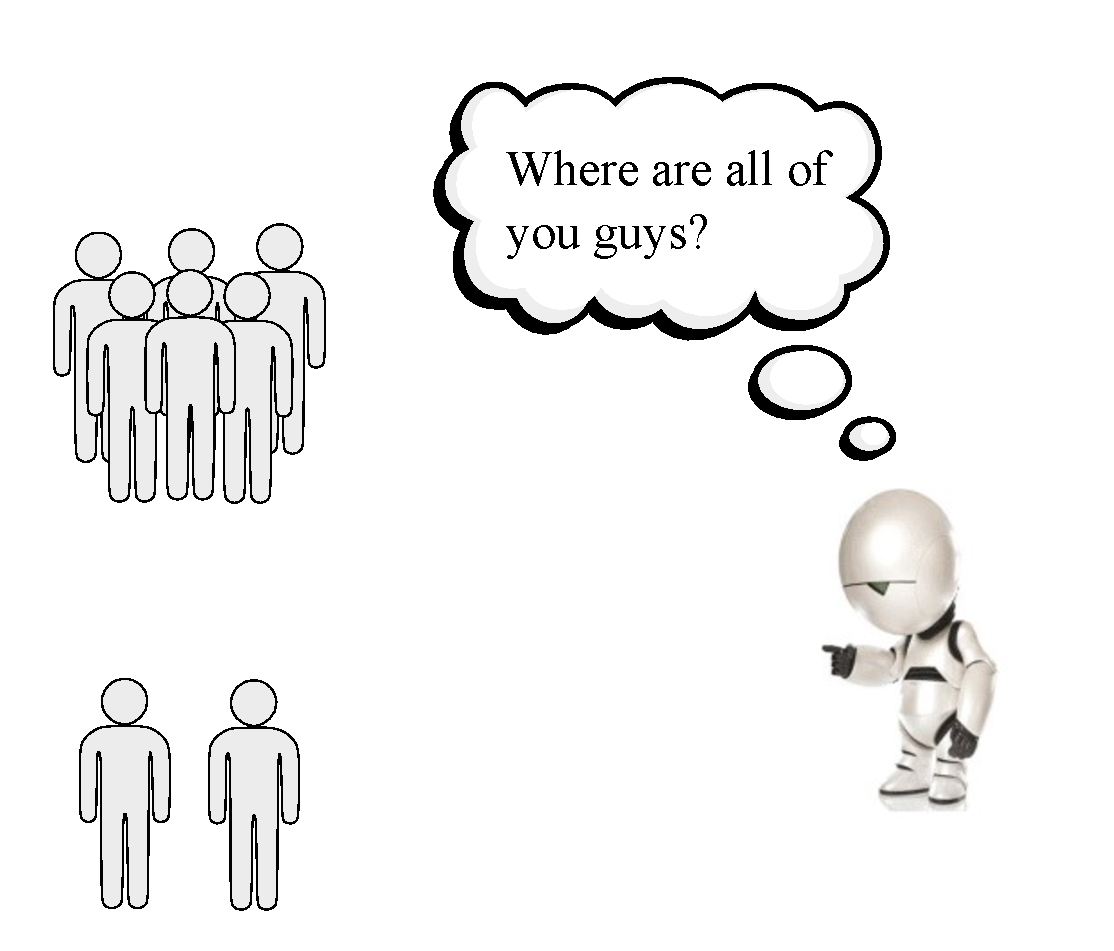
\includegraphics[width = 100mm]{Abbildungen/titelbild_1_0.pdf}


\vfill }
\end{spacing}
\begin{spacing}{1}
\begin{tabular}{l}
 \Large{Studienarbeit S-01/2021-997}
% Die einzutragende Nummer gibt es beim Betreuer!
\end{tabular}

\vspace{5mm}

\begin{tabular}{l}
\large{\Autor}\\
\large{Matrikelnummer \Matrikelnummer}
\end{tabular}

\vspace{5mm}

\begin{tabular}{l}
\large{Hannover, \Datum}
\end{tabular}


\vspace{5mm}
{\large
\begin{tabular}{l l}
Prüfer & Prof. Dr.-Ing. Tobias Ortmaier\\
Betreuer    & Marvin Stüde, M.Sc.\\
\end{tabular}
}

\end{spacing}
\end{titlepage}
\cleardoublepage %Titelseite
		
\includepdf[angle=180]{Vorlagen/selbst_signed.pdf} % Selbstständigkeitserklärung
    \clearpage
		%
\includepdf[pages=2]{Vorlagen/aufgabenstellung.pdf} % Aufgabenstellung als pdf einbinden
		
\includepdf{Vorlagen/kurzfassung_signed.pdf}
		%\newpage
\pdfbookmark[0]{Vortext}{frontmatter}
     \begin{flushright}
          \vspace*{-20mm}
          
\includegraphics[width=\textwidth]{Abbildungen/CoverLogos.pdf}
     \end{flushright}
\vspace*{10mm} % mit \usepackage{printlen}: 1.8cm * \uselengthunit{cm}\printlength{\textwidth} / 16.01cm = -1.773cm -> passt nicht, 10mm durch optik
{\let\clearpage\relax}\thispagestyle{empty}\pdfbookmark[1]{Aufgabenstellung}{aufgabenstellung}

\begin{spacing}{1}        
\begin{center}
\large\textbf{Zeit- und Ortsabhängige Prädiktion von Umweltzuständen für die Vorhersage von Personen- Auftrittswahrscheinlichkeiten}

\normalsize \Autor, Matrikelnummer \Matrikelnummer

\end{center}

\textbf{Allgemeines:}

Am Campus Maschinenbau in Garbsen wird der Serviceroboter Sobi entwickelt, welcher Studenten und Besuchern Informationen bereitstellen und bei der Orientierung auf dem Campusgelände helfen soll. Um eine möglichst hohe Rate an Mensch-Roboter-Interaktionen zu erreichen, muss der Roboter Informationen über das zeit- und ortsabhängige Personenaufkommen auf dem Campusgelände zur Verfügung haben. Diese Informationen können für die Bahnplanung verwendet werden, um die voraussichtlich benötigte Zeit einer Kontaktaufnahme mit einem Menschen zu minimieren. In der Forschung existieren Modelle zur Prädiktion dieser Umweltzustände auf Basis von binären sowie quantitativen Darstellungen.

\bigskip\textbf{Aufgabe:}

Im Rahmen dieser Arbeit soll eine Methodik entwickelt und für den spezifischen Anwendungsfall am Maschinenbau-Campus Garbsen angepasst werden. Als Ansatz einer solchen Methodik kann das FreMEn- Modell dienen. Die Grundidee der Methode ist die Transformation binärer zeit- und ortsabhängiger Darstellungen elementarer Umweltzustände (in diesem Fall die Anwesenheit bzw. Nichtanwesenheit von Personen) in den Frequenzbereich mittels der Fouriertransformation. In diesem werden die dominantesten Frequenzen identifiziert und auf Basis dieser eine inverse Fouriertransformation durchgeführt. Als Ergebnis erhält man eine Funktion, welche die Wahrscheinlichkeit für die zukünftigen Umweltzustände angibt. \\

Im Rahmen dieser Arbeit ergeben sich insbesondere die folgenden Aufgabenpunkte:

\begin{itemize}
	\item{Literaturrecherche über Methoden der binären sowie quantitativen Darstellung von Umweltzuständen}
	\item{Entwicklung einer Methodik und Anpassung an den vorliegenden Anwendungsfall}
	\item{Überprüfung der Modellgüte bei unterschiedlichen Periodendauern mittels eines Testdatensatzes}
	\item{Überprüfung der Modellgüte bei unterschiedlichen Periodendauern mittels eines Simulations- Datensatzes oder eines Langzeitdatensatzes}
	\item{Ermittlung weiterführender Fragestellungen zur Optimierung der kurzfristigen Vorhersagegüte des Modells}
\end{itemize}

Die Bearbeitungszeit beträgt 300 Stunden.

\vfill
\begin{center}
\begin{tabular}{p{0.35\textwidth} p{0.35\textwidth}}
Ausgabe der Aufgabenstellung:&15.06.2020\\
Abgabe der Arbeit spätestens am:&15.01.2021\\
Erstprüfer: \\
Zweitprüfer: \\
Betreuer: M. Sc. Marvin Stüde
\end{tabular}
\end{center}

\end{spacing}
% Leerseite einfügen
\cleardoublepage % Aufgabenstellung aus LaTeX nutzen
		%\chapter*{Kurzfassung}
\thispagestyle{empty}
In der Kurzfassung sollen auf maximal einer Seite die Aufgabe, die verwendeten Methoden sowie die erzielten Erkenntnisse dargestellt werden. Ein Leser soll idealerweise anhand der Kurzfassung abschätzen können, ob die Arbeit für ihn brauchbare Informationen enthält.

% Leerseite einfügen
\cleardoublepage
    \setcounter{page}{1}
    \pdfbookmark[0]{\contentsname}{toc}
    \tableofcontents                        % Inhaltsverzeichnis
    \listoffigures
    \listoftables
		%---------------------------------------------------------------------------------------------------------------------------
\chapter*{Nomenklatur}
\pdfbookmark{Nomenklatur}{}
%---------------------------------------------------------------------------------------------------------------------------
Selten bzw. nur abschnittsweise verwendete Symbole und Formelzeichen sowie abweichende Bedeutungen werden ausschließlich im Text beschrieben.
%---------------------------------------------------------------------------------------------------------------------------
\subsubsection{Allgemeine Konventionen}\vspace{-3mm}
%---------------------------------------------------------------------------------------------------------------------------
\begin{tabbing}
	1234567890 \= \kill
	Skalar \> Klein- oder Großbuchstabe (kursiv): $a$, $A$    \\
	Vektor \> Kleinbuchstabe (fett und kursiv): $\vec{a}$     \\
	Matrix \> Großbuchstabe (fett und kursiv): $\vec{A}$      \\
	Punkt  \> Klein- oder Großbuchstabe: $\ind{a}$, $\ind{A}$ \\            
\end{tabbing}
%---------------------------------------------------------------------------------------------------------------------------
%\subsubsection{Lateinische Buchstaben}\vspace{-3mm}
%---------------------------------------------------------------------------------------------------------------------------
%\begin{tabbing}
%	1234567890 \= \kill
	%------------------------------------------------------------------------------------------------------------------------
%	$A$																		\> %Querschnittsfläche \\
%	$A_\ind{S}$                           \> Spanungsquerschnitt \\
%	und so weiter
%\end{tabbing}
%---------------------------------------------------------------------------------------------------------------------------
%\subsubsection{Griechische Buchstaben}\vspace{-3mm}
%---------------------------------------------------------------------------------------------------------------------------
%\begin{tabbing}
%	1234567890 \= \kill
%	$\alpha, \ \beta, \ \gamma$												  \> %Rotationswinkel um die $x$"~, $y$"= und %$z$"=Achse                                         \\	
%\end{tabbing}
%---------------------------------------------------------------------------------------------------------------------------
\subsubsection{Koordinatensysteme}\vspace{-3mm}
%---------------------------------------------------------------------------------------------------------------------------
\begin{tabbing}
	1234567890 \= \kill
	$(\ind{KS})_{\mathcal{U}}$							        \> Koordinatensystem der Umgebung $\mathcal{U}$ \\
	%$\ks{0}$							        				\> ortsfestes %Inertialkoordinatensystem \\
\end{tabbing}
%---------------------------------------------------------------------------------------------------------------------------
\subsubsection{Abkürzungen}\vspace{-3mm}
% adrian : noch einfügen
%---------------------------------------------------------------------------------------------------------------------------
\begin{tabbing}
	1234567890 \= \kill
	FreMEn  \> Frequency Map Enhancement \\
	FFT		\> Fast Fourier Transformation \\
	DFT		\> Diskrete Fourier-Transformation \\
	GMM		\> Gaussian Mixture Models \\
\end{tabbing}
                    % Beschreibungen der verwendeten Abkürzungen und Variablen
    \mainmatter                             % der eigentliche Tex
    \setcounter{page}{1} % bei i anfangen
    \chapter{Einleitung}
Mobile Roboter finden immer mehr Einzug in die heutige Zeit. Als Beispiele seien mobile Staubsaug-Roboter oder Rasenmäh-Roboter sowie mobile Serviceroboter, welche mit Menschen interagieren können, zu nennen. All diesen verschiedenen Roboterarten liegt die Gemeinsamkeit zugrunde, dass sie für die effektive Bearbeitung ihrer Aufgaben auf eine modellierte Repräsentation ihrer Umgebung angewiesen sind. Für eine solche Umgebungsrepräsentation bestehen verschiedene Ansätze. Einige dieser Ansätze stellen die Umgebung als statisch dar \cite{Lakemeyer.2003}.  Dieser Ansatz kann für Anwendungsfälle wie einen Rasenmäher-Roboter, welcher wiederholt ein statisches Gebiet abfahren muss, genügen. Eine wesentliche Aufgabe mobiler Serviceroboter ist hingegen die Interaktion mit Personen innerhalb der Umgebung. Die Positionen dieser Personen sind dabei im Allgemeinen nicht statisch, sondern variieren mit der Zeit. Um seinen Aufgaben effektiv nachkommen zu können, benötigt der mobile Serviceroboter ein Modell der zeitlich und örtlich variablen Auftrittswahrscheinlichkeiten von Personen innerhalb seiner Arbeitsumgebung. Mithilfe eines solchen Modells ist der Roboter in der Lage, zu bestimmten Zeitpunkten gezielt Orte mit einem hohen Personenaufkommen anzufahren. Strebt der Roboter eine Kontaktaufnahme an, soll so die Zeit bis zum Erreichen dieser, gegenüber dem Abfahren einer zufälligen Route oder einem Verbleib und dem Warten an der aktuellen Position, reduziert werden. \\
In dieser Arbeit wird die Möglichkeit einer frequenzbasierten Modellierung zur Prädiktion von Personen-Auftrittswahrscheinlichkeiten untersucht. Neben einem binären Modell, welches die Auftrittswahrscheinlichkeiten von Personen prognostiziert, wird ein quantitatives Modell untersucht, welches die Anzahl von Personen innerhalb eines Zeitintervalls vorhersagen soll.  \\
In Kapitel 2 (Grundlagen und Stand der Technik) wird  auf die benötigten mathematischen Grundlagen eingegangen. Es werden Wahrscheinlichkeitsverteilungen und Funktionen vorgestellt, mittels derer binäre und quantitative Zustände modelliert werden können. Darauf aufbauend wird der aktuelle Stand der Technik im Bereich der binären und quantitativen Zustandsmodellierung präsentiert. Ein Hauptbestandteil des Kapitels ist die FreMEn (Frequency Map Enhancement) Methode. Die Methode modelliert Umweltzustände, wie das Personenaufkommen in einer Umgebung, durch zeitlich veränderliche Funktionen. Es erfolgt eine Untersuchung des Frequenzspektrums dieser zeitlich veränderlichen Funktionen und eine Approximation durch periodische, harmonische Funktionen \cite{Krajnik.2014}. \\
% Vllt. noch was zu Jovan schreiben?
In Kapitel 3 (Methodik) wird auf den Modellierungsprozess eingegangen. Es erfolgt eine Beschreibung der Messdatenermittlung und Vorverarbeitung durch ein Belegtheitsgitter, jeweils für binäre Zustandsmodelle sowie quantitative Zustandsmodelle. Im weiteren Verlauf des Kapitels wird die Server-Client-Struktur des Modells beschrieben. Der Client speichert die vorverarbeiteten Daten und schickt sie an den Server, welcher eine Frequenzanalyse der Daten durchführt und die zeitlich veränderlichen Funktionen durch eine Superposition periodischer, harmonischer Funktionen approximiert. Die ermittelten Parameter werden an den Client zurückgesendet, welcher diese speichert. \\
% Sollte ich das noch in das Kapitel 'Evaluation' schreiben? Vllt. mit einer nicen Grafik?
Kapitel 4 (Evaluation) evaluiert das binäre und quantitative Modell mittels zweier Datensätze. Es werden einheitliche Fehlermaße zur Bewertung der Modellgüten definiert. Darauf aufbauend erfolgt ein Vergleich der Modellgüten der binäre und quantitativen Modelle mit statischen Modellen, welche Umweltzustände durch zeitlich invariable, konstante Werte approximieren. Neben Möglichkeiten der Modelle wird auch auf limitierende Faktoren eingegangen. \\
In Kapitel 5 (Zusammenfassung und Ausblick) werden die gesammelten Ergebnisse zusammengefasst. Es erfolgt ein Ausblick auf weiterführende Fragestellungen im Rahmen der frequenzbasierten Modellierung von Personen-Auftrittswahrscheinlichkeiten.										% die einzelnen Kapitel einbinden
    	%\chapter{Grundlagen}
% Mal schauen, ob man die Bilder noch besser einfügen kann hier
% Und bei jedem Bild die referenzierte Quelle angeben
In diesem Kapitel werden die mathematischen Grundlagen zum Verständnis der Arbeit vorgestellt. Während in Abschnitt \ref{sec:Fourierreihen und Fouriertransformation} auf die Darstellung periodischer Funktionen mittels Fourierreihen eingegangen wird, behandelt Abschnitt \ref{sec.Diskrete Fouriertransformation} die mathematische Formulierung der diskreten Fouriertransformation für abgetastete Signale und geht des Weiteren auf das Nyquist-Shannon-Abtasttheorem ein.\\
In Abschnitt \ref{sec.Wahrscheinlichkeitsverteilungen} folgt dann eine Erläuterung zu Wahrscheinlichkeitsverteilungen. Den Anfang bildet hier die Binomialverteilung (Abschnitt \ref{sec.Binomialverteilung}), bevor zuletzt die Poisson-Verteilung (Abschnitt \ref{sec.Poissonverteilung}) besprochen wird.

\section{Fourierreihen und Fouriertransformation}
% Quelle: Eichler 2006
% Warum werden hier die Fourierreihen mit Sinus-Termen beschrieben, aber später mit Cosinus-Termen?
% Konsistente Formelschreibweise: rho_n und a_n müssen einheitlich geschrieben werden
\label{sec:Fourierreihen und Fouriertransformation}
Periodische Signale tauchen in vielen Bereichen der Physik und Technik auf. Ein Signal bezeichnet hierbei eine Funktion, welche eine physikalische Größe in Abhängigkeit von der Zeit, dem Ort, oder einer anderen Variablen darstellt. Betrachtet man periodische Funktionen, so zeichnen sich diese durch ihre Periodendauer $T$ aus. Die gesamten Informationen des Signals dabei in einer Periode, so dass gilt: $f(t) = f(t+T)$. Jede periodische Funktion kann durch eine Überlagerung von Sinus- und Kosinusfunktionen unterschiedlicher Periodendauern $2 \pi n$ approximiert werden. Dargestellt werden kann dies durch eine Fourierreihe: 

\begin{equation}
	\label{eq:Fourierreihe}
	f(t) = \dfrac{a_0}{2} + \sum_{n=0}^N[a_n \cos(n \omega t) + b_n \sin(n \omega t)]
\end{equation}
Hierbei bezeichnet $\omega = 2 \pi / T$ die Kreisfrequenz der Grundschwingung. Im Allgemeinen geht $N \to \infty$. Die Konstanten $a_0,a_1 \dots a_n$ werden als gerade Fourierkoeffizienten bezeichnet, $b_1, b_2 \dots b_n$ hingegen als ungerade Fourierkoeffizienten. Dies leitet sich daraus ab, dass der Cosinus eine gerade und der Sinus eine ungerade Funktion ist. \\
Des Weiteren lässt sich eine Fourierreihe durch Sinusfunktionen mit unterschiedlichen Amplituden und Phasen beschreiben. Die Fourierreihe lautet dann:
\begin{equation}
	\label{eq:Fourierreihe_umgerechnet}
	f(t) = \rho_0 + \sum_{n=1}^{N} \rho_n \sin(n \omega t + \varphi_n)
\end{equation}
Die Grundfrequenz des Signals lautet $f_1 = 1/ T = \omega / 2 \pi$. Die weiteren Sinus- und Kosinusfunktionen der Fourierreihe besitzen Frequenzen $f_n = nf_1$, also ganzzahlige Vielfache der Grundfrequenz. Die Umrechnung von Gleichung \ref{eq:Fourierreihe} nach Gleichung \ref{eq:Fourierreihe_umgerechnet} erfolgt mithilfe der Definitionen:
\begin{equation}
	\label{eq:rho_0}
	\rho_0 = \frac{a_0}{2}
\end{equation}
\begin{equation}
	\label{eq:rho_n}
	\rho_n = \sqrt{a_n^2 + b_n^2}
\end{equation}
\begin{equation}
	\label{eq:phi_n}
	\Phi_n = \arctan(\frac{a_n}{b_n})
\end{equation}
Mit $\rho_0$ (\ref{eq:rho_0}) wird hierbei der Gleichanteil des Signals bezeichnet, $\rho_n$ (\ref{eq:rho_n}) steht für die Amplitude der \textit{n-ten} Frequenz und $\varphi_n$ (\ref{eq:phi_n}) für die Phasenverschiebung der \textit{n-ten} Frequenz. Ein Signal kann also durch sein Kosinus- und Sinusspektrum sowie durch sein Amplituden- und Phasenspektrum charakterisiert werden. 
% hier muss jetzt noch das Bild 52.1 eingefügt werden, welches das zeitliche Signal beschreibt, sowie Bild 52.2 mit dem Amplituden-und Phasenspektrum. Dann noch Erläuterungen dazu machen.
Grafisch veranschaulicht wird die Fourierreihe durch \bild{Fourier}. In der linken Grafik eingezeichnet ist ein periodisches Signal mit der Periodendauer T, für welches also $f(t) = f(t+T)$ gilt. In den beiden rechten Grafiken finden sich die das Gesamtsignal definierenden Frequenzen, mit ihren zugehörigen Amplituden $\rho$ und Phasenversätzen $\varphi$.
\begin{figure}[!ht]
	\centering
	\subfigure[]{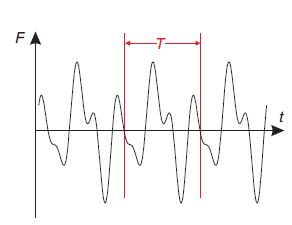
\includegraphics[height=50mm]{Abbildungen/grundlagen/signal}}
	\hspace{5mm}
	\subfigure[]{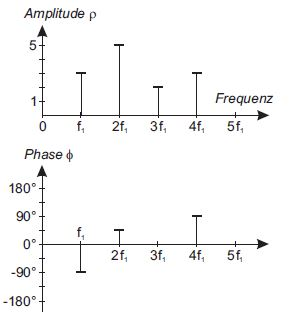
\includegraphics[height=50mm]{Abbildungen/grundlagen/amplituden_phasenspektrum}}
	\caption{Periodisches Signal mit zugehörigem Amplituden- und Phasenspektrum (Quelle: \cite{Eichler.2006}))}
	\label{fig.Fourier}
\end{figure}
\\
Die Fouriertransformation überführt die Gleichung aus dem Zeitbereich $f(t)$ nun in den Frequenzbereich $F(\omega)$. Für analoge Signale ist die Fouriertransformation nun wie folgt definiert:
\begin{equation}
	\label{eq:Fouriertransformation}
	F(\omega) = \int\limits_{-\infty}^{\infty} x(t) e^\ind{-j\omega} \ind{d}t.
\end{equation}
\begin{equation}
	\label{eq:Inverse_Fouriertransformation}
	f(t) = \frac{1}{2\pi}\int\limits_{-\infty}^{\infty} F(\omega)e^\ind{j\omega} \ind{d}\omega
\end{equation}
Gleichung \ref{eq:Fouriertransformation} überführt eine von der Zeit abhängige Funktion aus dem Zeitbereich über Integration von $-\infty$ bis $\infty$ über alle Zeitpunkte $t$ in den Frequenzbereich. Die inverse Fouriertransformation wird durch Gleichung \ref{eq:Inverse_Fouriertransformation} beschrieben. Die Rücktransformation erfolgt durch Integration von $-\infty$ bis $\infty$ des von der Frequenz $\omega$ abhängigen Signals über alle Frequenzen $\omega$ \cite{Eichler.2006}.

\section{Diskrete Fouriertransformation}
\label{sec.Diskrete Fouriertransformation}
% Quelle: Wendemuth
Die in Abschnitt \ref{sec:Fourierreihen und Fouriertransformation} dargestellten Gleichungen gelten für analoge Funktionen. In der Praxis ist es aber so, dass keine vollständige Kenntnis über ein Signal vorliegt, sondern dies nur durch Messungen zu diskreten Zeitpunkten abgetastet werden kann. Hieraus resultiert die Diskrete Fourier-Transformation (DFT). Die resultierenden Werte $F(n)$ der diskreten Fouriertransformation eines zu den Zeitpunkten $k$ abgetasteten Signals $f(t)$ können mittels Gleichung \ref{eq:DFT} berechnet werden. Die inverse diskrete Fouriertransformation erfolgt dann durch Gleichung \ref{eq:IDFT}.
\begin{equation}
	\label{eq:DFT}
	F(n) = \sum_{k=0}^{N-1}x[k]e^\ind{j\frac{2\pi}{N}kn}
\end{equation}
\begin{equation}
	\label{eq:IDFT}
	f[k] = \frac{1}{N}\sum_{k=0}^{N-1}F(n)e^\ind{j\frac{2\pi}{N}kn}
\end{equation} \\
Im Zusammenhang mit der Diskreten Fouriertransformation ist abschließend das Abtasttheorem von Nyquist und Shannon zu nennen. Das Theorem besagt, dass ein beliebig geformtes, kontinuierliches Signal immer dann durch ein diskretes Signal darstellbar und auch exakt wiederherstellbar ist, wenn die Abtastfrequenz des Signals mindestens doppelt so hoch ist, wie die höchste im kontinuierlichen Signal enthaltene Frequenz. Beträgt die höchste Frequenz in unserem Signal also beispielsweise \SI{10}{\Hz}, so müssen wir es mit mindestens \SI{20}{\Hz} abtasten, um das Signal vollständig rekonstruieren zu können  \cite{Wendemuth.2005}. \\
Die Folgen einer zu geringen Abtastfrequenz werden in \bild{Abtasttheorem} ersichtlich. Die Abtastung des Signals zu den mit schwarz markierten Zeitpunkten reicht nicht aus, um das in grau dargestellte Originalsignal zu rekonstruieren. Stattdessen ergibt sich das in rot dargestellte Signal.
% Diese Abbildung nochmal mit Inkscape nachbauen
\begin{figure}[!ht]
	\begin{center}
		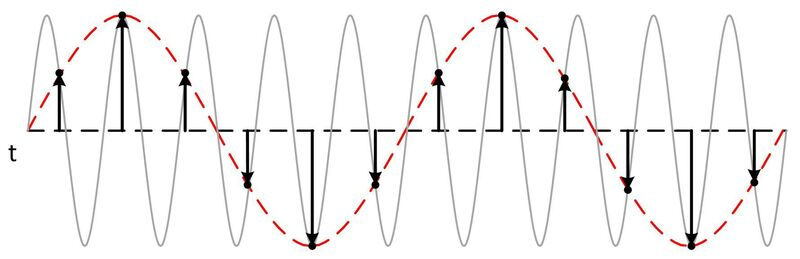
\includegraphics[height=50mm]{Abbildungen/grundlagen/abtasttheorem}
		\caption{Originalsignal (grau) und durch Abtastung rekonstruiertes Signal (rot) Quelle(https://www.geothermie.de/bibliothek/lexikon-der-geothermie/a/abtasttheorem.html)}
		\label{fig.Abtasttheorem}
	\end{center}
\end{figure}
\section{Wahrscheinlichkeitsverteilungen}
\label{sec.Wahrscheinlichkeitsverteilungen}
\subsection{Binomialverteilung}
\label{sec.Binomialverteilung}
% Quelle: Teschl 2010
Als Bernoulli-Experiment wird ein Zufallsexperiment bezeichnet, bei dem es lediglich zwei Ausgänge geben kann. Ein Ereignis A tritt entweder ein oder nicht. Führt man ein Bernoulli-Experiment n-mal hintereinander unter den gleichen Bedingungen durch, so erhält man eine Bernoulli-Kette der Länge $n$. Das Eintreten des Ereignisses A wird gemeinhin als Erfolg bezeichnet, die Wahrscheinlichkeit $P(A)=p$ bezeichnet man als Erfolgswahrscheinlichkeit. Als Ereignis A kann hier beispielhaft das Werfen einer Münze mit dem Ausgang $Zahl$ genannt werden. Eine Binomialverteilung entsteht nun, wenn wir die Anzahl der Erfolge bei einer Bernoulli-Kette ermitteln wollen. Mathematisch formuliert lässt sich die Binomialverteilung ausdrücken als:
\begin{equation}
	\label{eq:Binomialverteilung}
	P(X=x) = \binom{n}{x}p^\ind{x} q^\ind{n-x}
\end{equation}\\
$X$ bezeichnet hierbei die Anzahl der Versuchsdurchführungen, bei denen ein Erfolg eintritt. $X$ kann die Werte $x = 0,1,2,\dots,n$ annehmen, $p$ steht für die Eintrittswahrscheinlichkeit eines Erfolges, $q$ für die Wahrscheinlichkeit eines Misserfolges. Die Zufallsvariable $X$ ist binomialverteilt und ihre Wahrscheinlichkeitsverteilung eine Binomialverteilung mit den Parametern $n,p$. Kurz: $X \sim Bi(n;p)$. Die grafische Darstellung einer Binomialverteilung für die Wahrscheinlichkeit der Anzahl an Würfen eines Würfels mit dem Ereignis \textit{1} bei sieben Würfen ist in \bild{Poisson_Verteilung} dargestellt \cite{Teschl.2014}.
% Hier Bild aus Buch 2014 Mathe für Informatiker einfügen
% evtl noch Eigenschaften der Binomialverteilung einfügen? Oder unnötig?

\begin{figure}[!ht]
	\begin{center}
		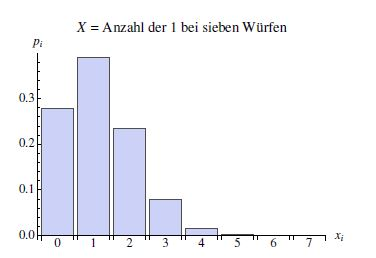
\includegraphics[height=50mm]{Abbildungen/grundlagen/Binomialverteilung}
		\caption{Binomialverteilung mit $n = 7, p = \frac{1}{6}$ Quelle \cite{Teschl.2014}}
		\label{fig.Poisson_Verteilung}
	\end{center}
\end{figure}
\subsection{Poissonverteilung}
\label{sec.Poissonverteilung}
Eine Zufallsvariable $X$, welche unendlich viele Werte $x=0,1,2\dots$ mit den Wahrscheinlichkeiten
\begin{align}
	P(X=x) &= \frac{\lambda^\ind{x}}{x!} e^\ind{-\lambda} & (\lambda >0)
	\label{eq:Poisson Verteilung}
\end{align}
annehmen kann, wird als poissonverteilt mit dem Parameter $\lambda$ bezeichnet. Die zugehörige Verteilung heißt Poisson-Verteilung. Der Erwartungswert sowie die Varianz der Poisson-Verteilung werden ausgedrückt als:
\begin{align}
	\mu &= E(X) = \lambda \\
	\sigma^2 &= Var(X) = \lambda
	\label{eq:Poisson EW und Var}
\end{align}
Anhand der obigen Formeln erkennt man, dass der Parameter der Poisson-Verteilung grade gleich ihres Erwartungswertes ist, selbiges gilt für die Varianz.
Häufig ist es von Interesse, die Anzahl $X_t$ eines Ereignisses innerhalb eines Zeitraumes $[0, t]$ zu prognostizieren. Die Menge von Zufallsvariablen $X_t, t\geq 0,$ wird als Poisson-Prozess mit der Intensität $\lambda$ bezeichnet, falls $X_t$ einer Poisson-Verteilung folgt, es also gilt: \\
\begin{equation}
	P(X_t=x) = \frac{(\lambda t)^x}{x!} e^\ind{-\lambda t}
	\label{eq:Poisson-Prozess}
\end{equation}
Ein Poisson-Prozess muss dabei nach \cite{Teschl.2014} drei Voraussetzungen erfüllen:
\begin{itemize}
	\item Die Wahrscheinlichkeit für ein Ereignis ist proportional zur Beobachtungsdauer $\Delta t$, aber unabhängig von der Lage des Beobachtungsintervalls.
	\item Die Wahrscheinlichkeiten für ein Ereignis an unterschiedlichen Orten sind voneinander unabhängig
	\item Für infinitesimal kleine $\Delta t$ ist die Wahrscheinlichkeit, dass das Ereignis mehr als einmal auftritt, im Vergleich zur Wahrscheinlichkeit, dass es genau einmal vorkommt, vernachlässigbar klein \cite{Teschl.2014}.
\end{itemize}

% Vllt noch eine Sektion zu GMM's (Gaussian Mixture Models) ? Wird in Paper Krajnik.2015b aufgegriffen. Evtl. Erklärung da etwas zu kurz gegriffen.



    	\chapter{Grundlagen und Stand der Technik}
\label{sec.Grundlagen und Stand der Technik}

In diesem Kapitel wird der aktuelle Stand der Technik zu Methoden der binären sowie quantitativen Darstellung von Umweltzuständen präsentiert. Es werden die mathematischen Grundlagen der in dieser Arbeit verwendeten Methoden behandelt. Neben Fourierreihen (Abschnitt \ref{sec.Fourierreihen und Fouriertransformation}) und der diskreten Fouriertransformation (Abschnitt \ref{sec.Diskrete Fouriertransformation}) wird  außerdem auf die Thematik der Wahrscheinlichkeitsverteilungen eingegangen. Aufgeführt wird neben der Binomialverteilung auch die Poissonverteilung (Abschnitt \ref{sec.Poissonverteilung}). \\
Darauf folgend werden Ergebnisse der Wissenschaft zur Beschreibung von Zustandsmodellen vorgestellt. Während Abschnitt \ref{sec.Beschreibung binärer Zustandsmodelle} sich mit der Beschreibung binärer Zustandsmodelle beschäftigt, legt Abschnitt \ref{sec.Beschreibung quantitativer Zustandsmodelle} den Fokus auf die Beschreibung quantitativer Zustandsmodelle. 

\section{Fourierreihen und Fouriertransformation}
\label{sec.Fourierreihen und Fouriertransformation}
Periodische Signale tauchen in vielen Bereichen der Physik und Technik auf. Ein Signal bezeichnet hierbei eine Funktion, welche eine physikalische Größe in Abhängigkeit von der Zeit, dem Ort, oder einer anderen Variablen darstellt \cite{Eichler.2006}. Betrachtet man periodische Funktionen, so zeichnen sich diese durch ihre Periodendauer $T$ aus. Eine Periode enthält dabei die gesamte Information des Signals, sodass gilt: $f(t) = f(t+T)$. Jede periodische Funktion kann durch eine Überlagerung von Sinus- und Kosinusfunktionen unterschiedlicher Periodendauern $2 \pi n$ approximiert werden \cite{Eichler.2006}. Dargestellt werden kann dies durch eine Fourierreihe 

\begin{equation}
	\label{eq:Fourierreihe}
	f(t) = \dfrac{a_0}{2} + \sum_{n=0}^N[a_n \cos(n \omega t) + b_n \sin(n \omega t)].
\end{equation}
Hierbei bezeichnet $\omega = 2 \pi / T$ die Kreisfrequenz der Grundschwingung. Die Konstanten $a_0,a_1 \dots a_n$ werden als gerade Fourierkoeffizienten bezeichnet, $b_1, b_2 \dots b_n$ hingegen als ungerade Fourierkoeffizienten. Dies leitet sich daraus ab, dass der Cosinus eine gerade und der Sinus eine ungerade Funktion ist. \\
Alternativ lässt sich eine Fourierreihe durch Sinusfunktionen mit unterschiedlichen Amplituden und Phasen beschreiben. Die Fourierreihe lautet dann
\begin{equation}
	\label{eq:Fourierreihe_umgerechnet}
	f(t) = \rho_0 + \sum_{n=1}^{N} \rho_n \sin(n \omega t + \varphi_n).
\end{equation}
Die Grundfrequenz des Signals lautet $f_1 = 1/ T = \omega / 2 \pi$. Die weiteren Sinus- und Kosinusfunktionen der Fourierreihe besitzen Frequenzen $f_n = nf_1$, also ganzzahlige Vielfache der Grundfrequenz. Die Umrechnung von Gleichung \ref{eq:Fourierreihe} nach Gleichung \ref{eq:Fourierreihe_umgerechnet} erfolgt mithilfe der Definitionen
\begin{equation}
	\label{eq:rho_0} 
	\rho_0 = \frac{a_0}{2} ,
\end{equation}
\begin{equation}
	\label{eq:rho_n}
	\rho_n = \sqrt{a_n^2 + b_n^2} ,
\end{equation}
\begin{equation}
	\label{eq:phi_n}
	\varphi_n = \arctan(\frac{a_n}{b_n}) .
\end{equation}
Mit $\rho_0$ wird hierbei der Gleichanteil des Signals bezeichnet, $\rho_n$ steht für die Amplitude der \textit{n}-ten Frequenz und $\varphi_n$ für die Phasenverschiebung der \textit{n}-ten Frequenz \cite{Eichler.2006}. Ein Signal kann also durch sein Kosinus- und Sinusspektrum sowie durch sein Amplituden- und Phasenspektrum charakterisiert werden. 
Grafisch veranschaulicht wird die Fourierreihe durch \bild{Fourier}. In Bild \ref{fig.Fourier_a} eingezeichnet ist ein periodisches Signal mit der Periodendauer $T$, für welches $f(t) = f(t + T)$ gilt. In Bild \ref{fig.Fourier_b} finden sich die das Gesamtsignal definierenden Frequenzen, mit ihren zugehörigen Amplituden $\rho$ und Phasenversätzen $\varphi$ \cite{Eichler.2006}.
\begin{figure}[!ht]
	\centering
	\subfigure[Periodisches Signal $F(t) = F(t + T $\label{fig.Fourier_a})]{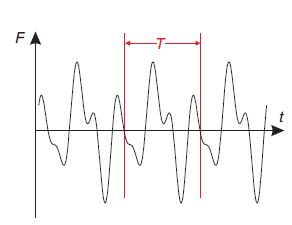
\includegraphics[height=50mm]{Abbildungen/grundlagen/signal}}
	\hspace{5mm}
	\subfigure[Amplituden- und Phasenspektrum des Signals\label{fig.Fourier_b}]{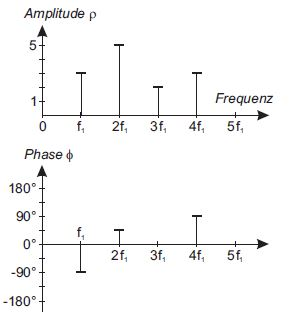
\includegraphics[height=50mm]{Abbildungen/grundlagen/amplituden_phasenspektrum}}
	\caption{Periodisches Signal mit zugehörigem Amplituden- und Phasenspektrum\, \cite{Eichler.2006}}
	\label{fig.Fourier}
\end{figure}
\\
Die Fouriertransformation überführt die Funktion $f(t)$ aus dem Zeitbereich in den Frequenzbereich. Für analoge Signale ist die Fouriertransformation definiert als
\begin{equation}
	\label{eq:Fouriertransformation}
	F(\omega) = \int\limits_{-\infty}^{\infty} f(t) e^\ind{-j\omega} \ind{d}t ,
\end{equation}
\begin{equation}
	\label{eq:Inverse_Fouriertransformation}
	f(t) = \frac{1}{2\pi}\int\limits_{-\infty}^{\infty} F(\omega)e^\ind{j\omega} \ind{d}\omega .
\end{equation}
Dieser Zusammenhang überführt eine, von der Zeit abhängige, Funktion aus dem Zeitbereich über Integration von $-\infty$ bis $\infty$ über alle Zeitpunkte $t$ in den Frequenzbereich. Die inverse Fouriertransformation erfolgt durch Integration von $-\infty$ bis $\infty$ des von der Frequenz $\omega$ abhängigen Signals über alle Frequenzen $\omega$ \cite{Eichler.2006}.

\section{Diskrete Fouriertransformation}
\label{sec.Diskrete Fouriertransformation}

Die in Abschnitt \ref{sec.Fourierreihen und Fouriertransformation} dargestellten Gleichungen gelten für zeitkontinuierliche Funktionen. In der Praxis ist es jedoch häufig so, dass keine vollständige Kenntnis über ein Signal vorliegt, sondern dieses nur durch Messungen zu diskreten Zeitpunkten abgetastet werden kann \cite{Eichler.2006}. Hieraus resultiert die Diskrete Fourier-Transformation (DFT). Die resultierenden Werte $F(n)$ der diskreten Fouriertransformation eines zu den Zeitpunkten $k$ abgetasteten Signals $f(t)$ berechnen sich durch 
\begin{equation}
	\label{eq:DFT}
	F(n) = \sum_{k=0}^{N-1}f[k]e^{j\frac{2\pi}{N}kn} .
\end{equation}

Die inverse diskrete Fouriertransformation (IDFT) erfolgt durch
\begin{equation}
	\label{eq:IDFT}
	f[k] = \frac{1}{N}\sum_{k=0}^{N-1}F(n)e^{j\frac{2\pi}{N}kn} .
\end{equation} \\
Im Zusammenhang mit der Diskreten Fouriertransformation ist abschließend das Abtasttheorem von Nyquist und Shannon zu nennen \cite{Eichler.2006}. Das Theorem besagt, dass ein beliebig geformtes, kontinuierliches Signal immer dann durch eine zu diskreten Zeitpunkten durchgeführte Abtastung darstellbar und auch exakt wiederherstellbar ist, wenn die zum Abtasten des Signals benutzte Frequenz mindestens doppelt so hoch ist, wie die höchste im kontinuierlichen Signal enthaltene Frequenz \cite{Wendemuth.2005}. Beträgt die höchste Frequenz in einem Signal also beispielsweise \SI{10}{\Hz}, so muss es mit mindestens \SI{20}{\Hz} abgetastet werden, damit das Signal vollständig rekonstruierbar ist  \cite{Wendemuth.2005}. \\
Die Folgen einer zu geringen Abtastfrequenz werden in \bild{Abtasttheorem} ersichtlich. Die Abtastung des Signals zu den mit schwarz markierten Zeitpunkten reicht nicht aus, um das in grau dargestellte Originalsignal zu rekonstruieren. Stattdessen ergibt sich das in rot markierte Signal.

\begin{figure}[!ht]
	\begin{center}
		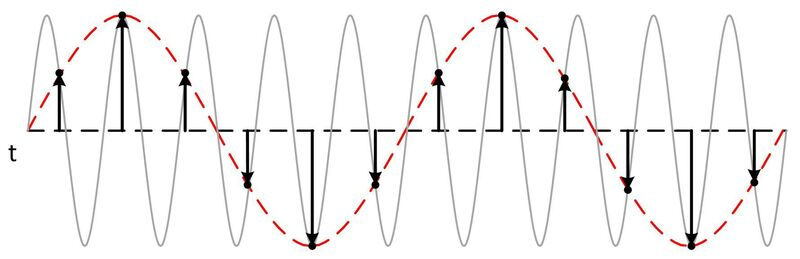
\includegraphics[width=1.0\linewidth,height=50mm]{Abbildungen/grundlagen/abtasttheorem}
		\caption[Originalsignal und durch Abtastung rekonstruiertes Signal]{Originalsignal (grau) und durch Abtastung rekonstruiertes Signal (rot)\, \cite{BBG.2020}
		}
		\label{fig.Abtasttheorem}
	\end{center}
\end{figure}

\section{Wahrscheinlichkeitsverteilungen}
\label{sec.Wahrscheinlichkeitsverteilungen}
% to-do: Einleitung hier reinschreiben. Warum brauchen wir Wahrscheinlichkeitsfunktionen überhaupt?
Dieser Abschnitt behandelt Wahrscheinlichkeitsverteilungen. Wahrscheinlichkeitsverteilungen werden benötigt, um Aussagen über das Ergebnis einer Aktion, wie beispielsweise den Ausgang eines Münzwurfes, zu treffen \cite{Teschl.2014}. Außerdem können mit ihrer Hilfe Aussagen über den Wert von Umweltzuständen für Zeitpunkte getroffen werden, zu denen dieser nicht direkt beobachtbar ist. Diese Aussagen werden dabei mit Hilfe gesammelter Informationen über vergangene Werte des Umweltzustandes getroffen \cite{Krajnik.2015}. Neben der Binomialverteilung wird im Folgenden auch auf die Poissonverteilung eingegangen. 
\subsection{Binomialverteilung}
\label{sec.Binomialverteilung}
% Einleitung zu Binomialverteilung schreiben

Ein Münzwurf mit seinen zwei möglichen Ausgängen \glqq{Kopf}\grqq{} beziehungsweise \glqq{Zahl}\grqq{} stellt ein Bernoulli-Experiment dar. Als Bernoulli-Experiment wird ein Zufallsexperiment bezeichnet, bei dem es lediglich zwei Ausgänge geben kann, ein Ereignis $A$ also entweder eintritt oder nicht \cite{Teschl.2014}. Führt man ein Bernoulli-Experiment $n$ -mal hintereinander unter den gleichen Bedingungen durch, so erhält man eine Bernoulli-Kette der Länge $n \in \mathbb{N}$. Das Eintreten des Ereignisses $A$ wird gemeinhin als Erfolg, die Wahrscheinlichkeit $P(A)=p$ \,  als Erfolgswahrscheinlichkeit bezeichnet \cite{Teschl.2014}. Als Ereignis $A$ kann beispielhaft das Werfen einer Münze mit dem Ausgang \glqq{$Zahl$}\grqq{} genannt werden. Eine Binomialverteilung entsteht, wenn man die Anzahl der Erfolge bei einer Bernoulli-Kette ermitteln will \cite{Teschl.2014}. Mathematisch formuliert lässt sich die Binomialverteilung ausdrücken als
\begin{equation}
	\label{eq:Binomialverteilung}
	P(X=x) = \binom{n}{x} \, p^{x} \, q^{n-x} .
\end{equation}\\
$X$ bezeichnet hierbei die Anzahl der Versuchsdurchführungen, bei denen ein Erfolg eintritt. $X$ kann die Werte $x = 0,1,2,\dots,n$\, annehmen, $p$ steht für die Eintrittswahrscheinlichkeit eines Erfolges, $q$ für die Wahrscheinlichkeit eines Misserfolges. Die Zufallsvariable $X$ ist binomialverteilt und ihre Wahrscheinlichkeitsverteilung eine Binomialverteilung mit den Parametern $n,p$ \cite{Teschl.2014}. Die grafische Darstellung einer Binomialverteilung für die Wahrscheinlichkeit der Anzahl an Würfen eines Würfels mit dem Ereignis \glqq{$1$}\grqq{} bei sieben Würfen ist in \bild{Poisson_Verteilung} dargestellt.

\begin{figure}[!ht]
	\begin{center}
		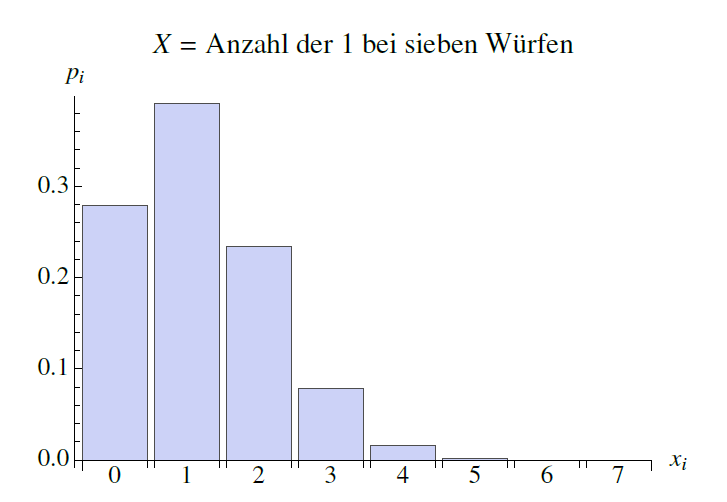
\includegraphics[height=50mm]{Abbildungen/grundlagen/Binomverteilung}
		\caption[Binomialverteilung Beispiel]{Binomialverteilung mit $n = 7, p = \frac{1}{6}$\,  \cite{Teschl.2014}}
		\label{fig.Poisson_Verteilung}
	\end{center}
\end{figure}
\subsection{Poissonverteilung}
\label{sec.Poissonverteilung}
% Einleitung schreiben
Es gibt viele Szenarien, in denen man sich für die Anzahl $X_t$ bestimmter Ereignisse innerhalb eines Zeitraumes interessiert. Beispielhaft können die Anzahl der Verkehrsunfälle pro Tag oder die Anzahl der Fertigungsfehler innerhalb einer Produktionstranche genannt werden \cite{Teschl.2014}. Zur stochastischen Beschreibung dieser Aufgabenstellungen eignet sich die Poisson-Verteilung \cite{Teschl.2014}.
Eine Zufallsvariable $X$, welche unendlich viele Werte $x=0,1,2\dots$ mit den Wahrscheinlichkeiten
\begin{align}
	P(X=x) = \frac{\lambda^{x}}{x!} e^{-\lambda}\qquad  \lambda >0
	\label{eq:Poisson Verteilung}
\end{align}
annehmen kann, wird als poissonverteilt mit dem Parameter $\lambda$ bezeichnet. Die zugehörige Verteilung heißt Poisson-Verteilung. Der Erwartungswert $\mu$ wird beschrieben durch 
\begin{equation}\label{eq:Poisson_EW}
	\mu = E(X) = \lambda ,
\end{equation}
die Varianz $\sigma ^2$ der Poisson-Verteilung berechnet sich zu
\begin{equation}\label{eq:Poisson_Var}
	\sigma^2 = Var(X) = \lambda .
\end{equation}
Anhand der obigen Formeln erkennt man, dass der Parameter der Poisson-Verteilung gleich ihres Erwartungswertes ist, selbiges gilt für die Varianz.
Häufig ist es von Interesse, die Wahrscheinlichkeit für eine Anzahl $X_t$ an Ereignissen innerhalb eines Zeitraumes $[0, t]$ zu bestimmen.
% Ein paar Beispiele nennen
Die Menge von Zufallsvariablen $X_t$ mit $ t\geq 0$ wird als Poisson-Prozess mit der Rate $\lambda$ bezeichnet, falls gilt
\begin{equation}
	P(X_t=x) = \frac{(\lambda t)^x}{x!} e^{-\lambda t} .
	\label{eq:Poisson-Prozess}
\end{equation}
Ein Poisson-Prozess muss dabei nach \cite{Teschl.2014} drei Voraussetzungen erfüllen:
\begin{itemize}
	\item Die Wahrscheinlichkeit für ein Ereignis ist proportional zur Beobachtungsdauer $\Delta t$, aber unabhängig von den Startzeitpunkten, also der zeitlichen Lage des Beobachtungsintervalls.
	\item Die Wahrscheinlichkeiten für ein Ereignis an unterschiedlichen Orten sind voneinander unabhängig.
	\item Für infinitesimal kleine $\Delta t$ ist die Wahrscheinlichkeit, dass das Ereignis mehr als einmal auftritt, im Vergleich zur Wahrscheinlichkeit, dass es genau einmal vorkommt, vernachlässigbar klein \cite{Teschl.2014}.
\end{itemize}

\section{Beschreibung binärer Zustandsmodelle}
\label{sec.Beschreibung binärer Zustandsmodelle}
Mobile Roboter finden immer mehr Einzug in Umgebungen, welche von Menschen bewohnt sind \cite{Krajnik.2017}. Diese Menschen üben Aktivitäten aus, welche in der Folge zu Veränderungen der Umgebung führen. Geht man davon aus, dass viele dieser Aktivitäten täglichen Routinen mit typischen Mustern folgen, kann man probieren, diese zu modellieren. Die Modelle können dann von mobilen Robotern zur robusteren Darstellung ihrer Umgebung genutzt werden. Das Mapping in statischen Umgebungen, also die Kartierung, stellt ein weit erforschtes Gebiet dar \cite{Lakemeyer.2003}.
Für das Mapping dynamischer Umgebungen gibt es verschiedene Ansätze. Während ein Ansatz darauf abzielt, sich bewegende Objekte aus der Umgebungsdarstellung herauszufiltern \cite{Hahnel.2002}, werden in anderen diese Objekte getrackt und als bewegte Landmarken klassifiziert \cite{Montesano.2008}. Diese separationsbasierten Ansätze können jedoch nicht auf Langzeitveränderungen der Umgebungsstruktur reagieren. \\
Im Gegensatz hierzu stehen adaptive Ansätze, welche davon ausgehen, dass der Prozess des Mappings niemals komplett abgeschlossen ist und dieser kontinuierlich aktualisiert werden muss. So können der Karte durch neue Observierungen des mobilen Roboters neue Features hinzugefügt werden 
\cite{Milford.2010}. In \cite{Krajnik.2014} wird versucht, die räumlich-zeitliche Dynamik einer Umgebung durch ihr Frequenzspektrum darzustellen. Die Werte von lokalen Umweltzuständen, wie zum Beispiel einer Tür, welche entweder offen oder geschlossen sein kann, sollen anhand von Wahrscheinlichkeitsfunktionen repräsentiert werden, welche aus der Superposition periodischer Funktionen resultieren. In \cite{Krajnik.2014} wird als Motivation dazu angeführt, dass bei den meisten Mapping-Ansätzen wichtige Umweltzustände lediglich statisch durch zwei eindeutige Zustände dargestellt werden. Eine Tür ist also entweder dauerhaft geöffnet oder geschlossen.
Diese Zustände können jedoch auch durch ihre Wahrscheinlichkeit ausgedrückt werden. Hierbei beschreibt $p_j$ die Wahrscheinlichkeit des $j$-ten Umweltzustandes einer Umgebung. Bayes-Filter gehen hierzu von einer statischen Welt aus, d.h. die Wahrscheinlichkeit des Zustandes $p_j$ wird als konstant angesehen. Durch neue Beobachtungen können diese konstanten Annahmen verändert werden, alte Beobachtungen werden so jedoch über die Zeit \emph{vergessen} \cite{Krajnik.2014}. Nimmt man an, dass diese Zustandswahrscheinlichkeiten $p_j (t)$ Funktionen der Zeit sind und diesen zeitlichen Veränderungen der Wahrscheinlichkeiten eine finite Anzahl periodischer Prozesse zu Grunde liegt, so könnte man den Einfluss und die Periodizität eben dieser Prozesse identifizieren und die Zustandswahrscheinlichkeit $p_j (t)$ aus dieser Beschreibung ermitteln. In \cite{Krajnik.2014} wird die in Abschnitt \ref{sec.Fourierreihen und Fouriertransformation} erläuterte Fouriertransformation benutzt, um diese periodischen Prozesse zu identifizieren. Als Beispiel wird ein Belegungsgitter herangeführt. Jede der Zellen des Belegungsgitters kann zwei Zustände $s_j = \{frei, belegt\}$ annehmen. Diese Zellzustände sind jedoch nicht konstant, sondern eine Funktion $s_j (t) $ der Zeit. Die Unsicherheit des Zustandes wird durch seine Wahrscheinlichkeit $p_j (t)$ ausgedrückt. Da die Zellen als unabhängig voneinander betrachtet werden, kann die Fouriertransformation separat auf jede Zelle des Belegungsnetzes angewendet werden. \\ Die über die Zeit aufgetragenen Zustände einer Zelle $s(t)$ werden mittels der Fouriertransformation $P = FT(s(t))$ transformiert. Es werden \textit{l} Koeffizienten $P_i$ des Spektrums $P$ ausgewählt und zusammen mit ihren Frequenzen $\omega_i$ benutzt, um mittels der inversen Fouriertransformation $p(t) = IFT(P'(t))$ die Wahrscheinlichkeitsfunktion $p(t)$ des Zellzustandes zu bestimmen. Die Menge $P$ besteht hierbei aus einer Anzahl von $l$ Tripeln mit den Einträgen $(abs(P_i), arg(P_i), \omega_i)$, wobei $abs(P_i)$ für die Amplitude, $arg(P_i)$ für den Phasenversatz und $\omega_i$ für die Frequenz des jeweiligen periodischen Prozesses steht, welcher den Zustand $s(t)$ beeinflusst. Anschließend wird ein Schwellwert benutzt, um aus $p(t)$ eine Schätzung $s'(t)$ der tatsächlichen Zustandsfunktion $s(t)$ zu bestimmen. \\

Der Zustand einer Zelle kann somit durch  
\begin{equation}
	s(t) = (IFT(P) > 0.5)
	\label{eq:Zellzustand}
\end{equation}
approximiert werden.

Ist die Wahrscheinlichkeit $p(t)$ einer Zellbelegung größer als 0.5, so wird die Zelle als belegt geschätzt.

Der in Gleichung \ref{eq:Zellzustand} benutzte Schwellwert von 0.5 kann willkürlich gesetzt werden. So können Vorhersagen über zukünftige Zustände der Zelle mit einem gewissen Konfidenzniveau von $c$ durch die Gleichung
\begin{equation}
	s'(t,c) = IFT(P) > c
	\label{eq:Zustandsvorhersage}
\end{equation}
getroffen werden. Diese Methode wird im Folgenden als Frequency Map Enhancement (FreMEn) bezeichnet. Grafisch verdeutlicht wird die Methode durch \bild{FreMEn Beispiel}. 

\begin{figure}[!ht]
	\begin{center}
		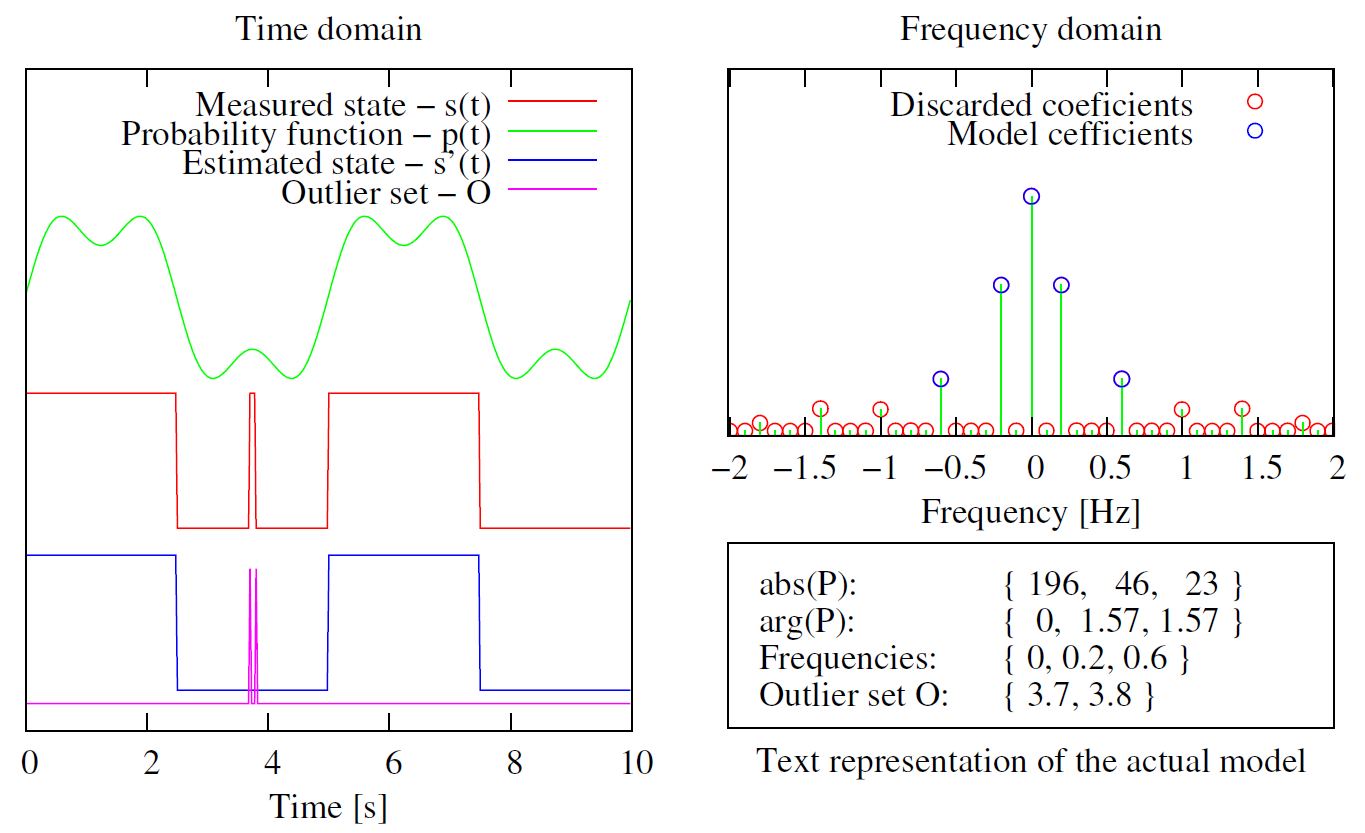
\includegraphics[height=70mm]{Abbildungen/stand_der_technik/example_of_measured_state_and_prediction}
		\caption{Beispiel eines über die Zeit gemessenen Zellzustandes sowie seines Spektralmodells und seiner Wahrscheinlichkeitsprädiktion\, \cite{Krajnik.2014}}
		\label{fig.FreMEn Beispiel}
	\end{center}
\end{figure}
% Outlier-Set beschreiben

In der linken Grafik rot dargestellt sind die, über einen zeitlichen Verlauf aufgenommenen, binären Zustände $s(t)$ einer Beispielzelle. Der grüne Graph beschreibt das zugehörige FreMEn-Modell $p(t)$ der Ordnung $l = 3$. Zur Konstruktion von $p(t)$ wurden somit drei periodische Prozesse verwendet. In blau aufgetragen sind die Vorhersagen $s'(t)$ des Modells, ermittelt anhand eines Schwellwertes von $c = 0.5$ \,. Der lila Graph stellt die Zeitpunkte dar, zu denen die Modellvorhersage von den tatsächlichen Zellzuständen abweicht \cite{Krajnik.2014}. Die rechte obere Grafik repräsentiert das Frequenzspektrum der Zelle, die für das Modell ausgewählten Frequenzen sind durch blaue Kreise markiert. Das zuvor erwähnte Tripel bestehend aus Amplitude, Phasenversatz und Frequenz der jeweiligen periodischen Prozesse ist in der rechten unteren Grafik dargestellt. Daneben findet sich hier auch die Menge der Ausreißer $\mathcal{O}$ mit den Zeitpunkten, zu denen die Modellvorhersage $s'(t)$ von den tatsächlichen Zellzuständen $s(t)$ abweicht.  Um die Auswirkungen des Modellgrades, also der Anzahl der in das Modell einfließenden periodischen Prozesse, zu erforschen, wurde die Methode auf einen Datensatz angewendet, bei welchem ein mobiler SCITOS-G5 Roboter, ausgestattet mit RGB-D und Lasersensoren, Personen in einem Bürogebäude über eine Dauer von einer Woche mit einer Frequenz von \SI{30}{\hertz} detektiert hat. \\
Die Genauigkeit des Modells $q(t_a,t_b)$ wird berechnet als
\begin{equation}
	q(t_a,t_b) = \frac{1}{t_b - t_a} \int_{t_a}^{t_b} |s'(t) - s(t)| \ind{d}t
	\label{eq:Modellgenauigkeit}
\end{equation}
und beschreibt das Verhältnis von korrekt geschätzten Zellzuständen zu der Gesamtdauer des betrachteten Intervalls.

Unterschieden wird in \cite{Krajnik.2014} nun zwischen der Rekonstruktionsgenauigkeit $q_\ind{r}$ sowie der Prädiktionsgenauigkeit $q_\ind{p}$. Die Rekonstruktionsgenauigkeit beschreibt, wie genau das Modell Zeitintervalle beschreibt, welche zur Ermittlung der Modellparameter verwendet wurden. Die Prädiktionsgenauigkeit hingegen beschreibt die Genauigkeit des Modells in Bezug auf Zeiträume, welche nicht zur Modellermittlung verwendet wurden. Die ermittelte Abhängigkeit der Rekonstruktions-sowie Prädiktionsgenauigkeit von der Modellordnung $l$ ist in \bild{predict_reconstruct_error} aufgezeigt. Hierbei erfolgte die Berechnung des Modells und der Rekonstruktionsgenauigkeit $q_\ind{r}$ anhand eines einwöchigen Datensatzes, die Evaluierung des Modells und die Ermittlung der Prädiktionsgenauigkeit $q_\ind{p}$ wurde mittels zwei externer Tage mit den zugehörigen Prädiktionsgenauigkeiten $q_\ind{p1}$ und $q_\ind{p2}$ durchgeführt.  \\

\begin{figure}[!ht]
	\begin{center}
		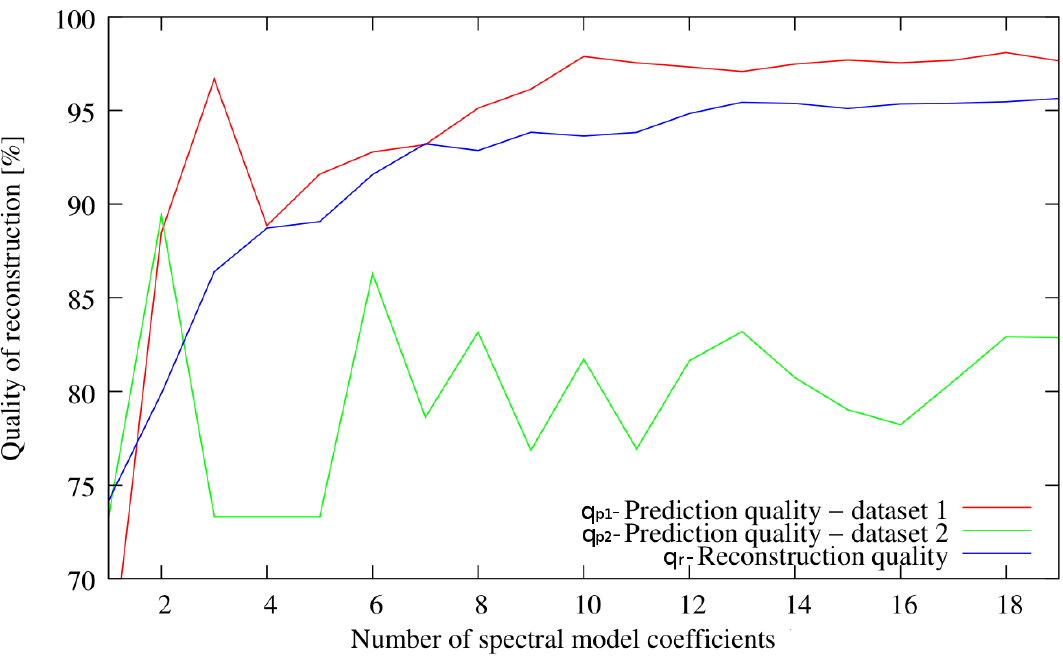
\includegraphics[width=0.7\linewidth]{Abbildungen/stand_der_technik/predict_reconstruct_error}
		\caption{Modellgenauigkeit vs. Modellordnung\,\cite{Krajnik.2014}}
		\label{fig.predict_reconstruct_error}	
	\end{center}
	
\end{figure}

Die Rekonstruktionsgenauigkeit liegt bei einer Modellordnung von $l=15$, d.h. es wurden 15 periodische Prozesse zum Approximieren des Zustandssignales verwendet, bei 95 \%. Die Rekonstruktionsgenauigkeit $q_\ind{r}$ steigt dabei monoton mit der Modellordnung. Für die Prädiktionsgenauigkeit $q_\ind{p}$ lässt sich nach \cite{Krajnik.2014} kein allgemeingültiger Zusammenhang finden. Während die Prädiktionsgenauigkeit des ersten Testtages bei $l=3$ ein lokales Maximum, bei $l=17$ jedoch ein globales Maximum besitzt, liegt das globale Maximum für den zweiten Testtag bei $l=2$.\\
Die lokalen Maxima von $q_\ind{p1}$ und $q_\ind{p2}$ lassen laut \cite{Krajnik.2014} den Schluss zu, dass für die Vorhersage eine Modellordnung von zwei oder drei optimal ist (siehe \bild{predict_reconstruct_error}). \\
Einen Vergleich zwischen der in \cite{Krajnik.2014} beschriebenen FreMEn- Methode und der Anwendung von periodischen Gauß-Mischmodellen zur Darstellung der Dynamik von binären Umweltzuständen zieht \cite{Krajnik.2015b}. FreMEn basiert hier, wie auch schon in \cite{Krajnik.2014} auf der Idee, die zeitliche Funktion $s(t)$ eines Umweltzustandes durch seine Wahrscheinlichkeitsfunktion $p(t)$ zu schätzen. Auch hier wird wieder mittels einer Fouriertransformation das Frequenzspektrum $S(\omega)$ der zeitlichen Funktion $s(t)$ bestimmt, und die \textit{l} prominentesten Frequenzen mit ihren Amplituden $a_j$, ihrem Phasenversatz $\varphi_j$ sowie ihrer Frequenz $\omega_j$ abgespeichert. Die Ermittlung der Wahrscheinlichkeit $p(t)$ eines Umweltzustandes zum Zeitpunkt \textit{t} ergibt sich durch die Superposition der \emph{l} Frequenzen zu
\begin{equation}
	p(t) = a_0 + \sum_{j=1}^{n} a_j \cos(\omega_j t + \varphi_j) .
	\label{eq:Superposition}
\end{equation}
Die erste spektrale Komponente $a_0$ stellt hierbei den Durchschnitt aller binären Werte von $s(t)$, also dessen Gleichanteil (siehe Abschnitt \ref{sec.Fourierreihen und Fouriertransformation}) dar. FreMEn besitze aber laut \cite{Krajnik.2015b} zwei wesentliche Nachteile. So erlaube es zum einen, lediglich einen periodischen Prozess pro Frequenz zu modellieren. Des Weiteren bilde es wiederkehrende, aber kurze, Prozesse schlecht ab. Als Beispiel wird hier die morgendliche Dusche angeführt, welche eine tägliche, aber kurze Routine sei. Da in \cite{Krajnik.2014} herausgearbeitet wurde, dass die optimale Modellordnung $l_\ind{opt}$ für eine möglichst hohe Prognostiziergenauigkeit bei einer Größe von lediglich zwei bis drei liegt, könnten solche kurzen Routinen nicht abgebildet werden. \\ Als zweiter Ansatz werden Gaussian Mixture Models (GMM) genannt. Diese können multidimensionale Funktionen als gewichtete Summe aus mehreren Gauß-Funktionen durch
\begin{equation}
	f(t) = \frac{1}{\sqrt{2 \pi}} \sum_{j=1}^{m} \frac{\omega_j}{\sigma_j} e^{- \frac{(t- \mu_j)^2}{2 \sigma_j ^2}}
	\label{eq:Gaussian_Mixture_Models}
\end{equation}
approximieren.
Die Parameter der individuellen Komponenten eines GMM, namentlich das Gewicht $\omega_j$, der Durchschnitt $\mu_j$ sowie die Standardabweichung $\sigma_j$ werden typischerweise mittels Trainingsdaten anhand des Iterative Expectation Maximization (EM) oder des Maximum A-Posteriori (MAP) Algorithmus ermittelt. Während GMM in der Lage sind, Funktionen jeglichen Aussehens zu modellieren, liegt ihre Limitation darin, dass sie definitionsgemäß keine periodischen Funktionen repräsentieren können \cite{Krajnik.2015b}. Um diesem Problem entgegenzuwirken, wird vorab eine Periodendauer von einem Tag vorgegeben. Diese Vorgabe erlaubt es, die gemessene Sequenz der Umweltzustände $s(t)$  in eine Sequenz $p'(t)$ umzuwandeln mit
\begin{equation}
	p'(t) = \frac{k}{\tau} \sum_{i=1}^{\frac{k}{\tau}} s(t+i \tau) .
	\label{eq:GMM_sequence}
\end{equation}
In Gleichung (\ref{eq:GMM_sequence}) bezeichnet $\tau$ die vorab definierte Periodendauer, $k$ beschreibt die Länge der Sequenz $s(t)$. Nach Anwendung des Expectation Maximization Algorithmus kann die Wahrscheinlichkeit für einen Umweltzustand berechnet werden zu
\begin{equation}
	p(t) = \frac{1}{\sqrt{2 \pi}} \sum_{j=1}^{m} \frac{w_j}{\tau_j} e ^{- \frac{(mod(t,\tau) - \mu_j)^2}{2 \sigma_j^2}} .
	\label{eq:Gauss_Probability}
\end{equation}
Hierbei beschreibt $\tau$ die vorgegebene Periodendauer der Funktion $p(t)$ und $mod$ ist der Modulo-Operator. Dass die Stärken und Schwächen dieser periodischen GMM-basierten (PerGaM) Modelle komplementär zu jenen der FreMEn-Methodik sind, wir anhand von \bild{PerGaM_vs_FreMEn} deutlich.
\begin{figure}[!ht]
	\begin{center}
		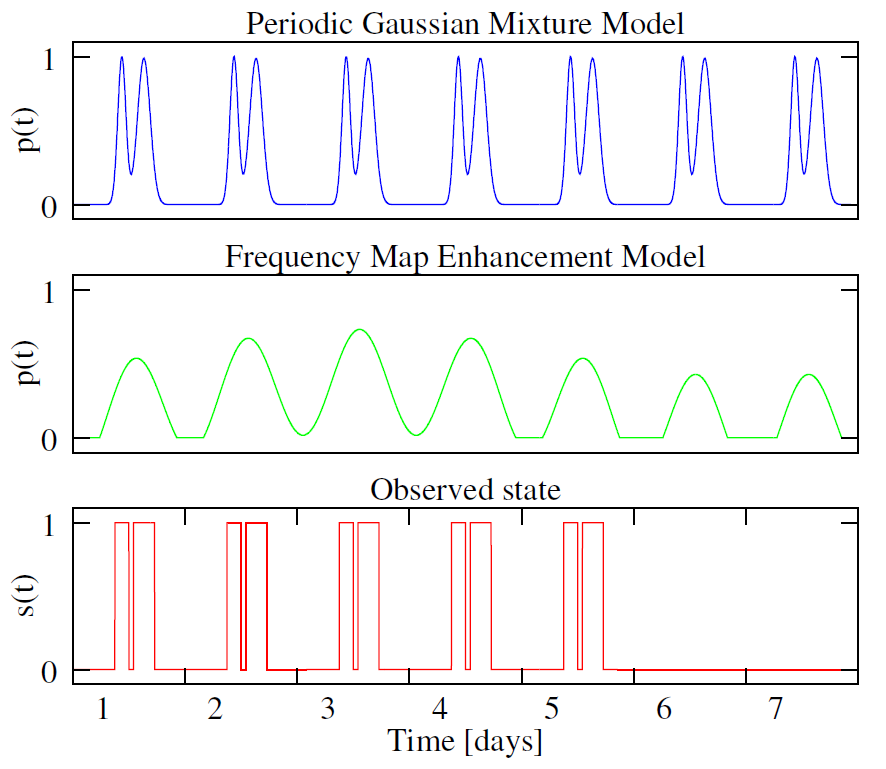
\includegraphics[width=0.7\linewidth]{Abbildungen/stand_der_technik/PerGaM_vs_FreMEn}
		\caption{PerGaM und FreMEn Modellvergleich\, \cite{Krajnik.2015b}}
		\label{fig.PerGaM_vs_FreMEn}
	\end{center}
\end{figure}
Das PerGaM-Modell kann selbst kurze, mehrfach auftretende Routinen approximieren, jedoch kann es lediglich eine Periodendauer repräsentieren, welche a priori bekannt bzw. festgelegt werden muss. Als Resultat werden kurzzeitige Routinen, wie z.B. Mittagspausen, gut approximiert, die wöchentliche Dynamik mit dem Fehlen von Personen am Wochenende kann hingegen nicht modelliert werden. Im Vergleich dazu sieht man das FreMEn-Modell, welches die Wochendynamik durch ein Abflachen der Signalamplitude an den beiden Wochenendtagen abbildet (siehe \bild{PerGaM_vs_FreMEn}). \\
In Bezug auf das zeitlich-räumliche Mapping durch mobile Roboter führt \cite{Krajnik.2015} an, dass dies auch eine räumlich-zeitliche Explorationsstrategie benötigt. Im Vergleich zu klassischen Explorationsstrategien, bei denen, bedingt durch die endliche Größe der zu erforschenden Karte, die Exploration ebenfalls finit ist, sei die Exploration dynamischer Umgebungen niemals abgeschlossen. Vielmehr würde die räumlich-zeitliche Exploration Teil der täglichen Routine des Roboters werden.
Es stellt sich ein wesentlicher Nachteil der in \cite{Krajnik.2014} vorgestellten Methode zur Darstellung von binären Umweltzuständen in Bezug auf die kontinuierliche Exploration einer Karte durch einen mobilen Roboter heraus. Diese beruht auf der traditionellen Fast Fourier Transformation (FFT). Die Fast Fourier Transformation kann jedoch lediglich die komplette Sequenz eines Umweltzustandes $s(t)$ in sein Frequenzspektrum $S(\omega)$ transformieren. Außerdem erfordert der Algorithmus, dass die Zustandsobservierungen mit der immer gleichen Frequenz aufgenommen werden.  Orte mit der immer selben Frequenz zu erkunden, sei jedoch nicht effizient, sodass in \cite{Krajnik.2015} eine neue Methode zur Darstellung von binären Umweltzuständen durch zeitlich variable Wahrscheinlichkeitsfunktionen vorgestellt wird. Die Methode erlaubt ein inkrementelles und kontinuierliches Aktualisieren des räumlich-zeitlichen Umgebungsmodells durch wenige Observierungen, welche zu unterschiedlichen, nicht gleichmäßig verteilten Zeitpunkten, und an unterschiedlichen Orten aufgenommen werden können. \\
Jeder Umweltzustand $s(t)$ wird durch die Anzahl getätigter Observierungen $n$, seines Durchschnittes $\mu$ sowie zwei Sets $A,B$ komplexer Zahlen $\alpha_k$ und $\beta_k$, welche zu dem Set $\Omega$ periodischer Prozesse $\omega_k$ gehören, die den Umweltzustand beeinflussen, beschrieben. Anfangs wird der Wert $\mu$ jedes Umweltzustandes zu $\mu = 0.5$ und alle $\alpha_k$ sowie $\beta_k$ zu 0 gesetzt, was einem vollkommen unbekannten Zustand entspricht. Die inkrementelle Aktualisierung des Modells erfolgt durch 
\begin{align}
	\mu &\leftarrow \frac{1}{n+1}(n \mu + s(t)), \\
	\alpha_k &\leftarrow \frac{1}{n+1} (n \alpha_k + s(t) e^{-jt\omega_k}) ,  &\forall \omega_k \in \Omega, \\
	\beta_k &\leftarrow \frac{1}{n+1} (n \beta_k + \mu e^{-jt\omega_k}) ,  &\forall \omega_k \in \Omega, \\
	n &\leftarrow n + 1 .
	\label{eq:Update_step_FreMEn}
\end{align}
Die schrittweise Aktualisierung entspricht dabei einer inkrementellen Mittelwertbildung. Der Betrag $\gamma_k = |\alpha_k - \beta_k|$ stellt den durchschnittlichen Einfluss des periodischen Prozesses $k$ auf den Umweltzustand $s(t)$ dar.
Wären die Zeitpunkte $t$ der Observationen und die Frequenzen $\omega_k$ gleichmäßig verteilt, so entsprächen die obigen Formeln der diskreten Fouriertransformation.
Um den zukünftigen Wert eines Umweltzustandes prognostizieren zu können, werden wie auch in \cite{Krajnik.2014} die $m$ periodischen Prozesse mit den höchsten absoluten Werten $|\gamma_k|$ ausgewählt. Die Wahrscheinlichkeit eines Umweltzustandes wird mittels
\begin{equation}
	p(t) = \varsigma(\mu + \sum_{l=1}^{m} |\gamma_l|\cos(\omega_k t + arg(\gamma_l)))
	\label{eq:State_probability}
\end{equation}
berechnet. Die Funktion $\varsigma(.)$ sorgt dafür, dass $p(t) \in [0,1]$ gilt. Der optimale Wert für $m$ wird wie schon in \cite{Krajnik.2014} so gewählt, dass die Prädiktionsgenauigkeit $q_\ind{p}$ maximiert wird. \\

\section{Beschreibung quantitativer Zustandsmodelle}
\label{sec.Beschreibung quantitativer Zustandsmodelle}
% Einleitung quantitativer Zustandsmodelle
Aus Abschnitt \ref{sec.Beschreibung binärer Zustandsmodelle} wurde ersichtlich, dass
binäre Zustandsmodelle Aussagen über die Wahrscheinlichkeit $p(t)$ eines Zellzustandes, wie z.B. die Belegtheit einer Zelle $s(t)$, erlauben. Möchte man jedoch Schätzungen für die Anzahl, wie oft eine Zelle innerhalb eines Zeitintervalls belegt bzw. besucht wird, treffen, so ist dies nur durch eine quantitative Zustandsbeschreibung möglich.
Eine Methode zur Modellierung von quantitativen Umweltzuständen wird in \cite{Jovan.2016} vorgestellt. Die hier genannte Methode beruht auf der Kombination von zeitveränderlichen Poisson-Prozessen und einer Frequenzanalyse. Dabei wird die Häufigkeit des Auftretens eines Ereignisses innerhalb eines Zeitintervalls gezählt. Anders ausgedrückt wird gezählt, wie häufig ein Umweltzustand, beispielsweise das Vorhandensein einer Person in einer Zelle, den Wert \emph{wahr} pro Zeitintervall annimmt. Somit kann anstatt der Wahrscheinlichkeitsfunktion $p(t)$ eines Umwelt- bzw. Zellzustandes dessen Intensität bzw. Rate innerhalb des Zeitintervalls dargestellt werden. Diese Raten $\lambda (t)$ werden mit Hilfe von Poisson-Prozessen modelliert. Wie schon  in Abschnitt \ref{sec.Poissonverteilung} beschrieben, wird auch hier die Poisson-Verteilung mittels
\begin{equation}
	P(N;\lambda) = \frac{e^\ind{-\lambda} \lambda^N}{N!}, \qquad	N=0,1,2,\dots
\end{equation}

berechnet, wobei $P(N;\lambda)$ die Wahrscheinlichkeit $P$ für den Fall beschreibt, dass innerhalb eines Zeitintervalls $\Delta t_i$ mit einer durchschnittlichen Aktivitätenanzahl, also einer durchschnittlichen Personenanzahl von $\lambda$, exakt $N$ Aktivitäten, also Personen, gezählt werden. Die Daten in \cite{Jovan.2016} wurden von einem mobilen Metralabs Scitos A5-Roboter aufgenommen, welcher sich, ausgestattet mit einem robusten Personen-Tracking-Algorithmus, einen Monat lang in einem Bürogebäude bewegte. Die Abhängigkeit der durchschnittlichen Personenanzahl $\lambda$ vom betrachteten Zeitintervall wird durch $\lambda (t_i, t_j)$ ausgedrückt, wobei  $t_i$ den Anfangszeitpunkt und $t_j$ den Endzeitpunkt des Intervalls beschreibt. Da die von dem Roboter aufgenommenen Daten nur einen kleinen Teil der Gesamtheit des Personenaufkommens repräsentieren, wird $\lambda$ mittels einer Konfidenz-basierten Schätzung bestimmt. Der Poisson-Parameter $\lambda$ folgt hierbei einer Gammaverteilung
\begin{equation}
	\lambda \sim \Gamma(\lambda ; \alpha, \beta) .
\end{equation}
Die a-posteriori Wahrscheinlichkeit für $\lambda (t_i, t_j)$ berechnet sich unter Berücksichtigung der aufgenommenen Daten zu
\begin{equation}
	P(\lambda | x_1, \dots, x_n) = \Gamma(\lambda, \alpha + \sum_{i=1}^{n} x_i, \beta +n) ,
\end{equation}
wobei $x_1, \dots , x_n$ die im betreffenden Intervall aufgezeichneten Daten bezeichnen, der Parameter $\alpha$ steht für den Formfaktor, $\beta$ für den inversen Skalenparameter der Gammaverteilung.
Der Datensatz wird in Wochen eingeteilt, für ein Zeitintervall wird eine Dauer von zehn Minuten gewählt. Die Maximum a posteriori-Wahrscheinlichkeit (MAP) jedes Parameters $\lambda(t_i, t_j)$ wird als Punktschätzung für $\lambda$ gewählt. Die Verknüpfung sämtlicher Punktschätzungen über den definierten Zeitraum einer Woche ergibt das Poisson-Prozess-Modell, welches in \bild{poisson-prozess-model1} grafisch aufgezeichnet ist. 
\begin{figure}[!ht]
	\begin{center}
		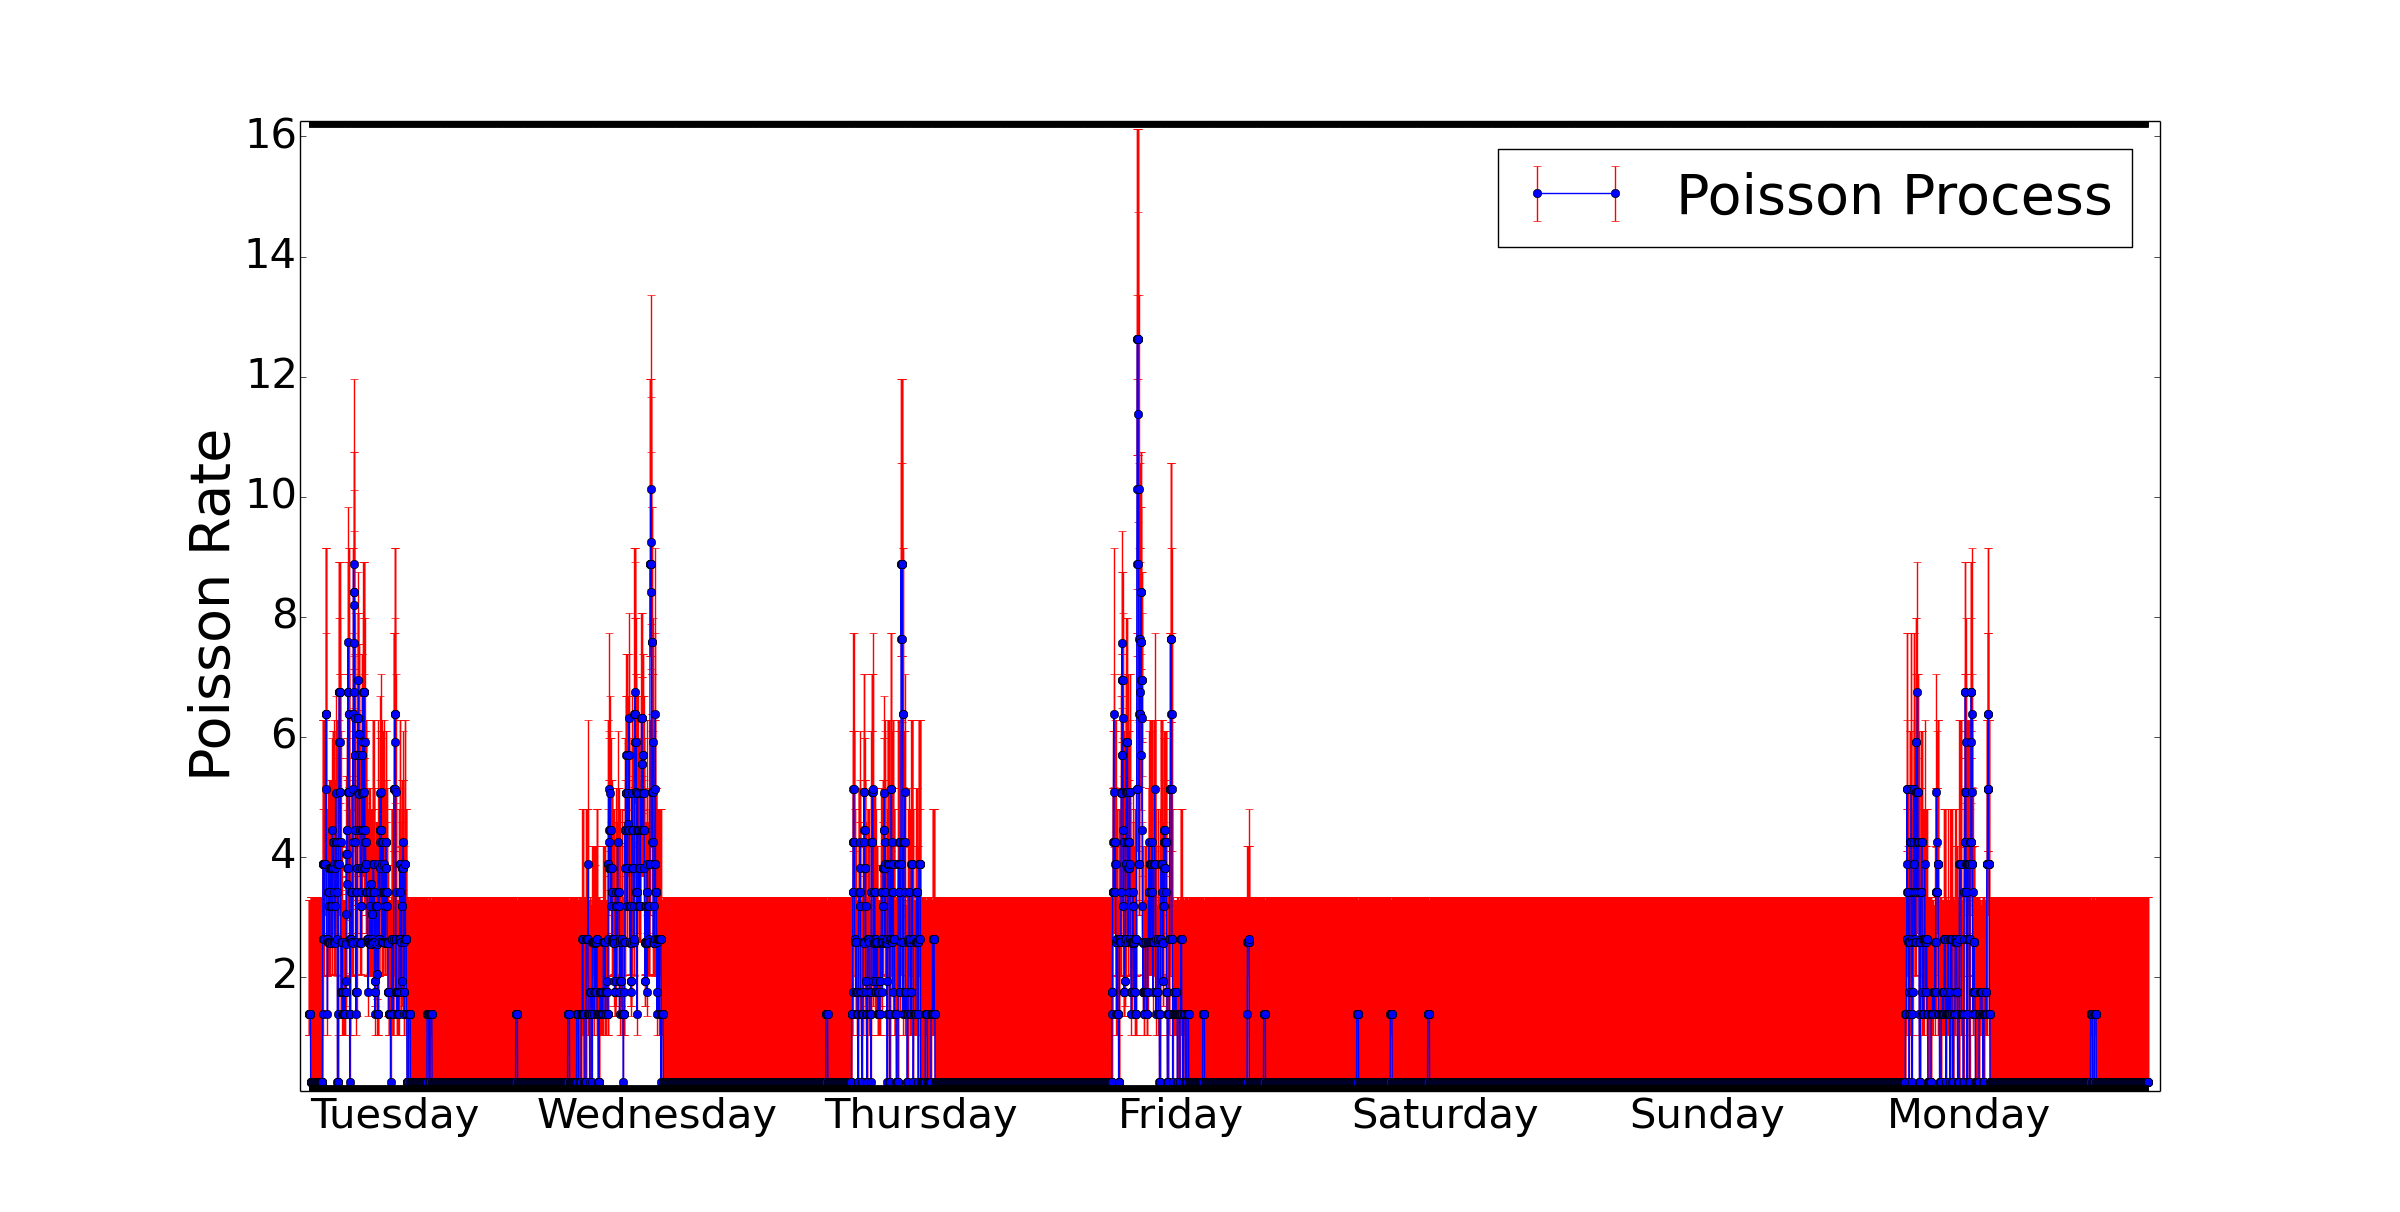
\includegraphics[width=0.8\linewidth]{Abbildungen/stand_der_technik/poisson-prozess-model1}
		\caption{Aktivitätsraten $\lambda$ des Poisson-Prozess-Modells ermittelt anhand eines 4 Wochen Zeitraumes\, \cite{Jovan.2016}}
		\label{fig.poisson-prozess-model1}
	\end{center}
\end{figure}

Für jedes $\lambda$ wurden die Daten von vier aufeinanderfolgenden Wochen verwendet, die roten Schranken zeigen die oberen und unteren Grenzen des Konfidenzintervalls für jedes $\lambda$. \\
Nach der Berechnung des Poisson-Prozess-Modells wird nun die Fouriertransformation auf $\lambda (t)$ angewendet. Ebenso wie in \cite{Krajnik.2014} werden die $l$ Frequenzen mit den höchsten Amplituden zur Konstruktion von $\lambda' = IFT(F'(\omega))$ verwendet. Im Gegensatz zu der in \cite{Krajnik.2014} durch Superposition der Parameter der $l$ prominentesten Frequenzen verwendeten und hier als \emph{l Best Amplitude Model} (BAM) bezeichneten Methode wird in \cite{Jovan.2016} die \emph{l Addition Amplitude Model} (AAM) Methode verwendet. Es wird angeführt, dass das BAM den Betrag des Original-Signals nicht komplett abbilden kann, sofern die Sampling-Rate der Daten deutlich höher ist als die höchste beobachtete Frequenz. \\ AAM hingegen berechnet das Fourierspektrum des Poisson-Prozess-Modells, findet die Frequenz $\omega_k$ mit der höchsten Amplitude und zieht es von den Daten ab. Die modifizierten Daten werden wieder transformiert und das Frequenzspektrum erneut berechnet. Findet sich in diesem Frequenzspektrum eine bereits vorher identifizierte Frequenz, so wird dessen neuerliche Amplitude auf die bereits vorhandene addiert, und die Daten erneut modifiziert. Dieses Vorgehen wird bis zur Identifikation der $l$ Frequenzen mit den höchsten Amplituden wiederholt. \bild{BAM_AAM_Vergleich} bietet einen Vergleich der beiden Methoden zur Abbildung des Poisson-Prozess-Modells. Aus der Grafik wird ersichtlich, dass das AAM die Beträge des Original-Modells deutlich besser abbilden kann als das BAM.

\begin{figure}[!ht]
	\centering
	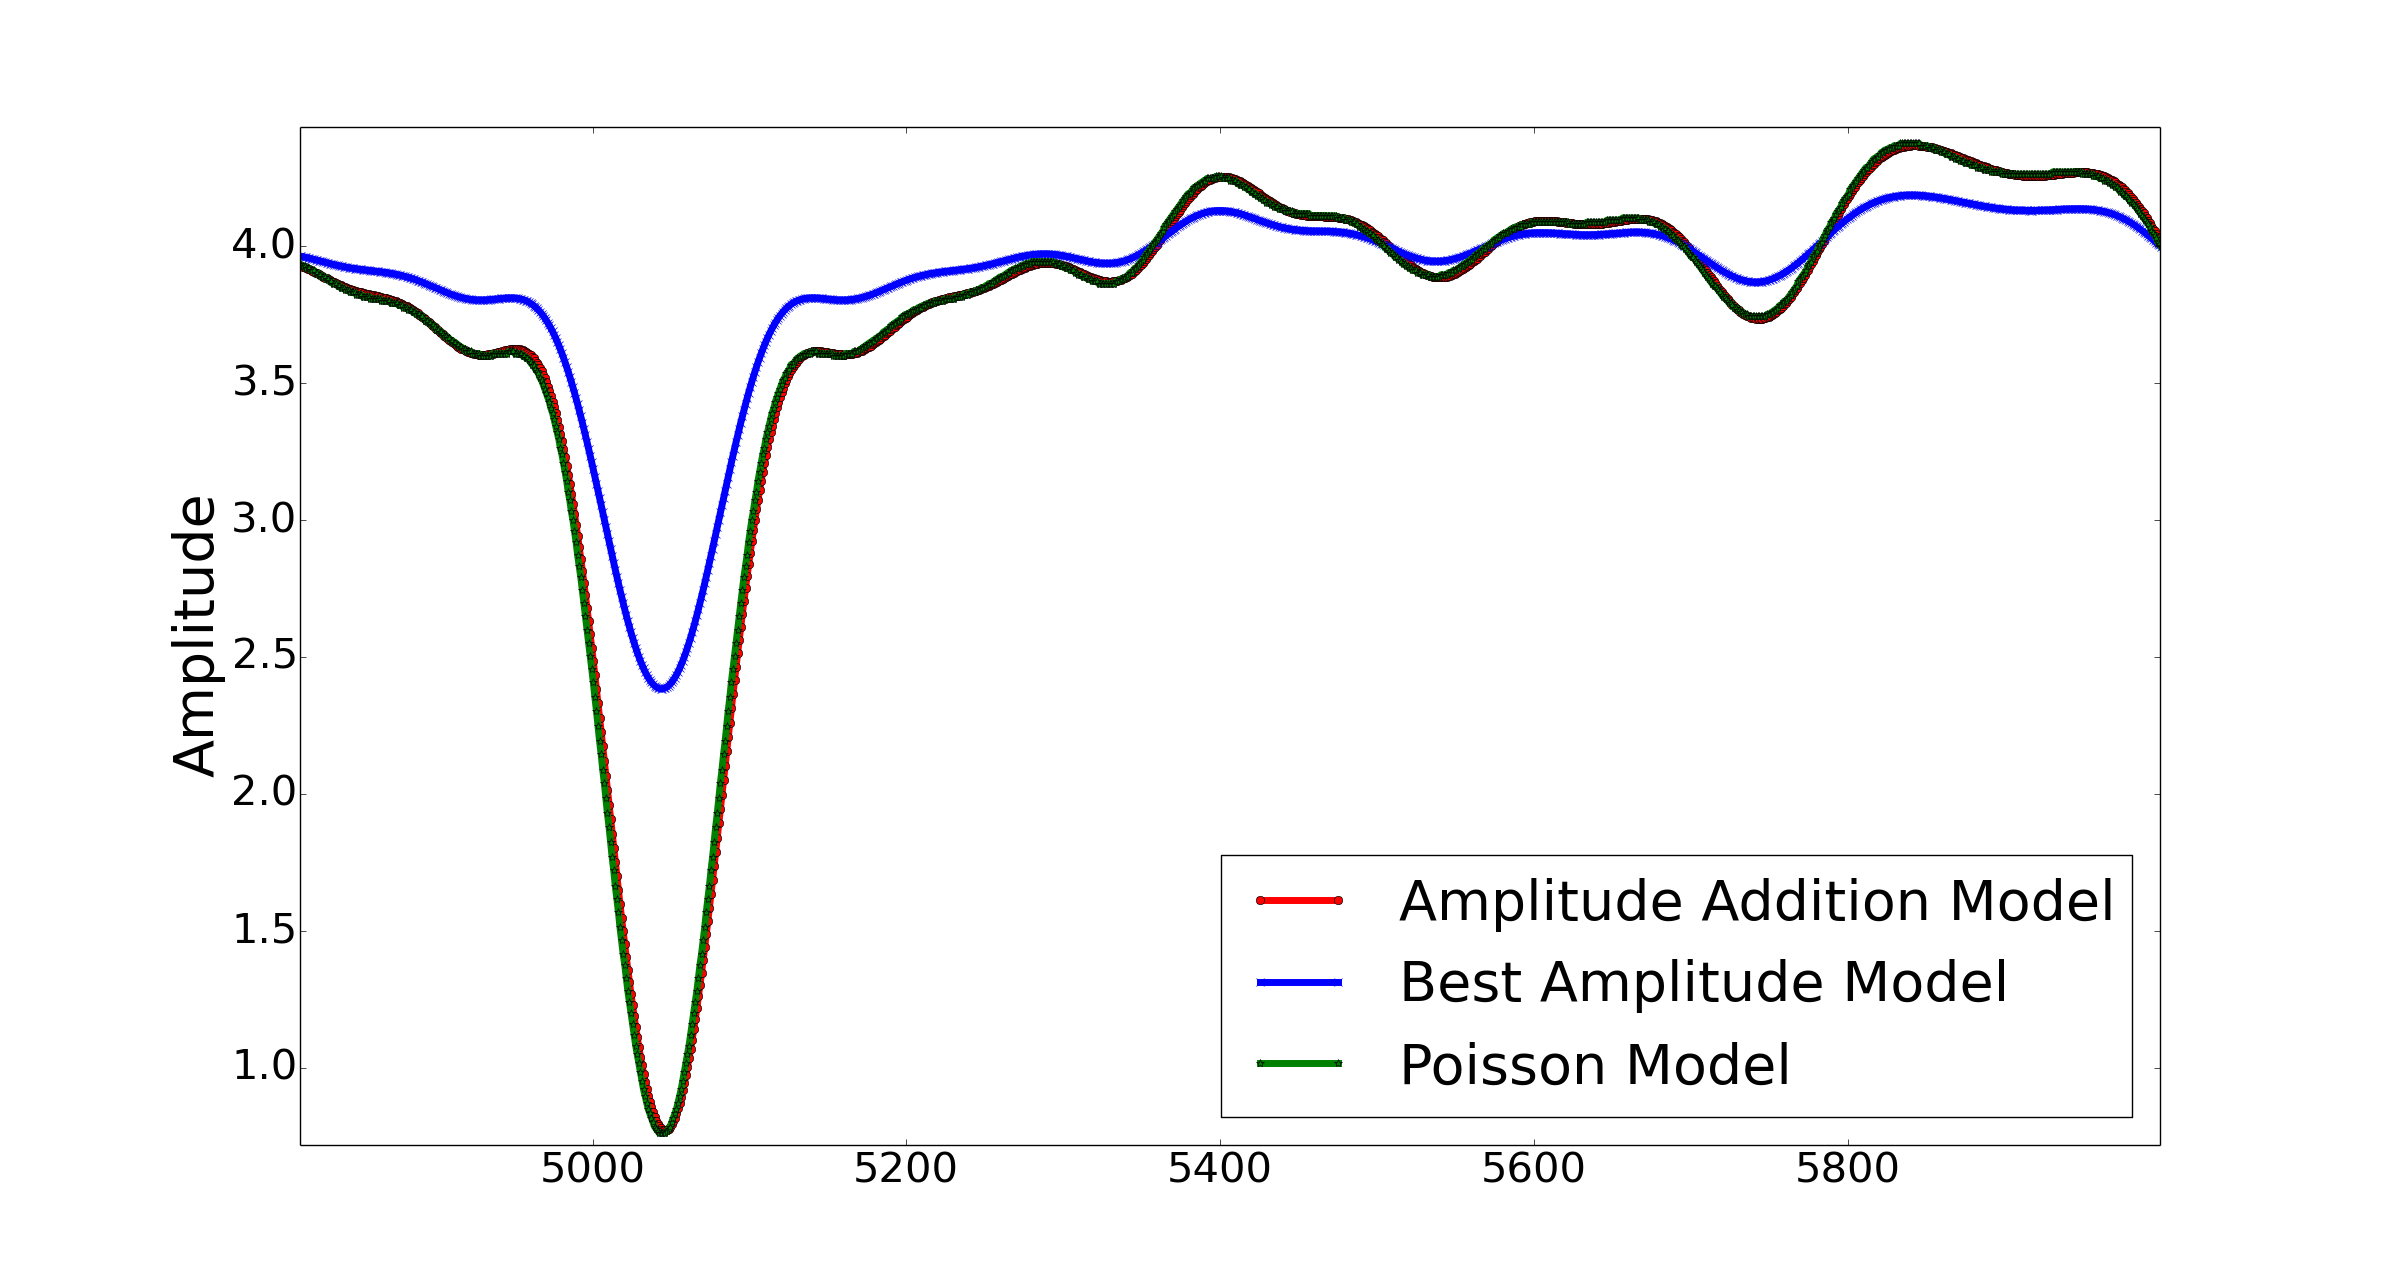
\includegraphics[width=0.8\linewidth]{Abbildungen/stand_der_technik/BAM_AAM}
	\caption{Vergleich \emph{l Best Amplitude Model} und \emph{l Addition Amplitude Model} \, \cite{Jovan.2016}}
	\label{fig.BAM_AAM_Vergleich}
\end{figure}

Eine genauere Beschreibung der Berechnung des Formfaktors $\alpha$ und des inversen Skalenparameters $\beta$ der Gammafunktion findet sich in \cite{Stuede.2020}. Hier wird der Parameter $\lambda$ für jede Zelle eines 2D-Gitters berechnet. Die Wahrscheinlichkeit
für die Anzahl $N$ an Aktivitäten innerhalb eines Zeitintervalls in einer Zelle des Gitters kann dargestellt werden über
\begin{equation}
	P_{ij \tau} (N(t) = k) = \frac{(\lambda_{ij \tau}(t-t_\tau))^k}{k!} e^{-\lambda_{ij\tau} (t- t_\tau)} ,
\end{equation}
wobei $\lambda_{ij \tau}$ für die Rate an Aktivitäten der Zelle $(i,j)$ innerhalb des Zeitintervalls $\tau$ steht. Die der Zelle und dem jeweiligen Intervall zugehörigen Parameter $\alpha_{ij\tau}$ sowie $\beta_{ij\tau}$ werden inkrementell für jeden Zeitschritt $\sigma$ bestimmt  mittels der Vorschrift
\begin{equation}
	\alpha_\sigma = \alpha_{\sigma - 1} + x_\sigma \boldsymbol{1}_\ind{\mathcal{D}} (\boldsymbol{x}_\ind{R}, t_\sigma),\qquad  \beta_\sigma = \beta_{\sigma - 1} + \boldsymbol{1}_\ind{\mathcal{D}} (\boldsymbol{x}_\ind{R}, t_\sigma ) .
\end{equation}
Als Anfangswerte werden $\alpha_0 = \beta_0 = 1 $ gewählt. Die Indikator-Funktion $\boldsymbol{1}_\ind{\mathcal{D}} (\boldsymbol{x}_r, t_\sigma)$ resultiert hierbei aus dem Detektionsbereich eines Roboters bei der Pose $\boldsymbol{x}_\ind{R}$. Die a-posteriori erwarteten Werte der Aktivitätenrate $\lambda$ und ihrer Varianz berechnen sich für jedes Intervall zu
\begin{equation}
	\hat{\lambda}_{ij\tau} = E[\lambda_{ij\tau}] = \frac{\alpha_{ij\tau}}{\beta_{ij}\tau},\qquad	Var[\lambda_{ij\tau}] = \frac{\alpha_{ij\tau}}{\beta_{ij\tau}^2} .
\end{equation}



    	\chapter{Methodik}
\label{sec.Methodik}
Dieses Kapitel behandelt die Methodik zur Prädiktion von Umweltzuständen. Die Beschreibung der verwendeten Methoden erfolgt separat für binäre Zustandsmodelle (Abschnitt \ref{sec.Binäre Zustandsmodelle}), bei denen die Wahrscheinlichkeit $p(t)$ für einen Umweltzustand, wie beispielsweise die Belegtheit $s(t)$ einer Zelle innerhalb eines geografischen Gitters, bestimmt werden soll, sowie für quantitative Zustandsmodelle (Abschnitt \ref{sec.Quantitative Zustandsmodelle}), bei denen Aussagen über die Anzahl an Ereignissen innerhalb einer Zelle während eines bestimmten Zeitintervalls getroffen werden sollen.
\section{Binäre Zustandsmodelle}
\label{sec.Binäre Zustandsmodelle}
Binäre Zustandsmodelle dienen, wie schon in Abschnitt \ref{sec.Beschreibung quantitativer Zustandsmodelle} erläutert, der Beschreibung einer Zustandsfunktion $s(t)$ durch eine Wahrscheinlichkeitsfunktion $p(t)$. In den folgenden Abschnitten werden die Schritte zur Bestimmung dieser Modelle durchgegangen. Werden in einem ersten Schritt die Messdaten eines Belegtheitsgitters ermittelt (Abschnitt \ref{sec.Messdatenermittlung eines Belegtheitsgitters binär}), so erfolgt in einem weiteren Schritt die Client-seitige Verarbeitung dieser Messdaten (Abschnitt \ref{sec.Verarbeitung client binär}), bevor die Daten an einen Server geschickt werden, auf welchem diese zur Erstellung binärer Zustandsmodelle verwendet werden (Abschnitt \ref{sec.Verarbeitung server binär}). 

\subsection{Messdatenermittlung eines Belegtheitsgitters}
\label{sec.Messdatenermittlung eines Belegtheitsgitters binär}
Den ersten Schritt der Methodik bildet die Aufzeichnung von Messdaten. Als Messdaten werden die Detektionen von Personen innerhalb einer Umgebung $\mathcal{U}$ bezeichnet. Eine Umgebung $\mathcal{U}$ ist ein geografisch abgegrenztes Gebiet, als Beispiele können hier ein Bürogebäude, ein Apartment oder ein offenes Gelände genannt werden. Die Ermittlung der Messdaten kann zum Beispiel durch einen, mit einem Personen-Detektions-Algorithmus ausgestatteten, mobilen Roboter erfolgen, oder durch mehrere, in $\mathcal{U}$ verteilte, statische Sensoren, welche ebenfalls das Auftreten von Personen detektieren können. Werden innerhalb eines Zeitraumes $T$ insgesamt $N$ Personen detektiert, also $N$ Messungen aufgezeichnet, so lässt sich die Gesamtheit der Messungen schreiben als
\begin{equation}
	\boldsymbol{X} = (\boldsymbol{x}_1, \boldsymbol{x}_2, \dots , \boldsymbol{x}_N)^\ind{T} .
	\label{eq:Gesamtheit Messungen}
\end{equation}
Die Messung einer einzelnen Personendetektion ist hierbei
\begin{equation}
	\boldsymbol{x}_i = (x_\ind{det}, y_\ind{det}, t_\ind{det})^\ind{T} .
	\label{eq:Einzelmessung_x}
\end{equation}
Eine Messung beinhaltet  die x-Position  $x_\ind{det}$ der Detektion innerhalb des Umgebungskoordinatensystems $(\textrm{KS})_\ind{\mathcal{U}}$, die y-Position $y_\ind{det}$ der Detektion innerhalb des Umgebungskoordinatensystems, sowie den Zeitstempel $t_\ind{det}$ der Detektion.
Für die weitere Betrachtung wird über die Umgebung $\mathcal{U}$ ein Gitter gelegt, welches aus diskreten, räumlich finiten Zellen besteht. Grafisch veranschaulicht ist dieses Verfahren in \bild{Bürogebäude_Gitter}.

\begin{figure}[!h]
	\begin{center}
		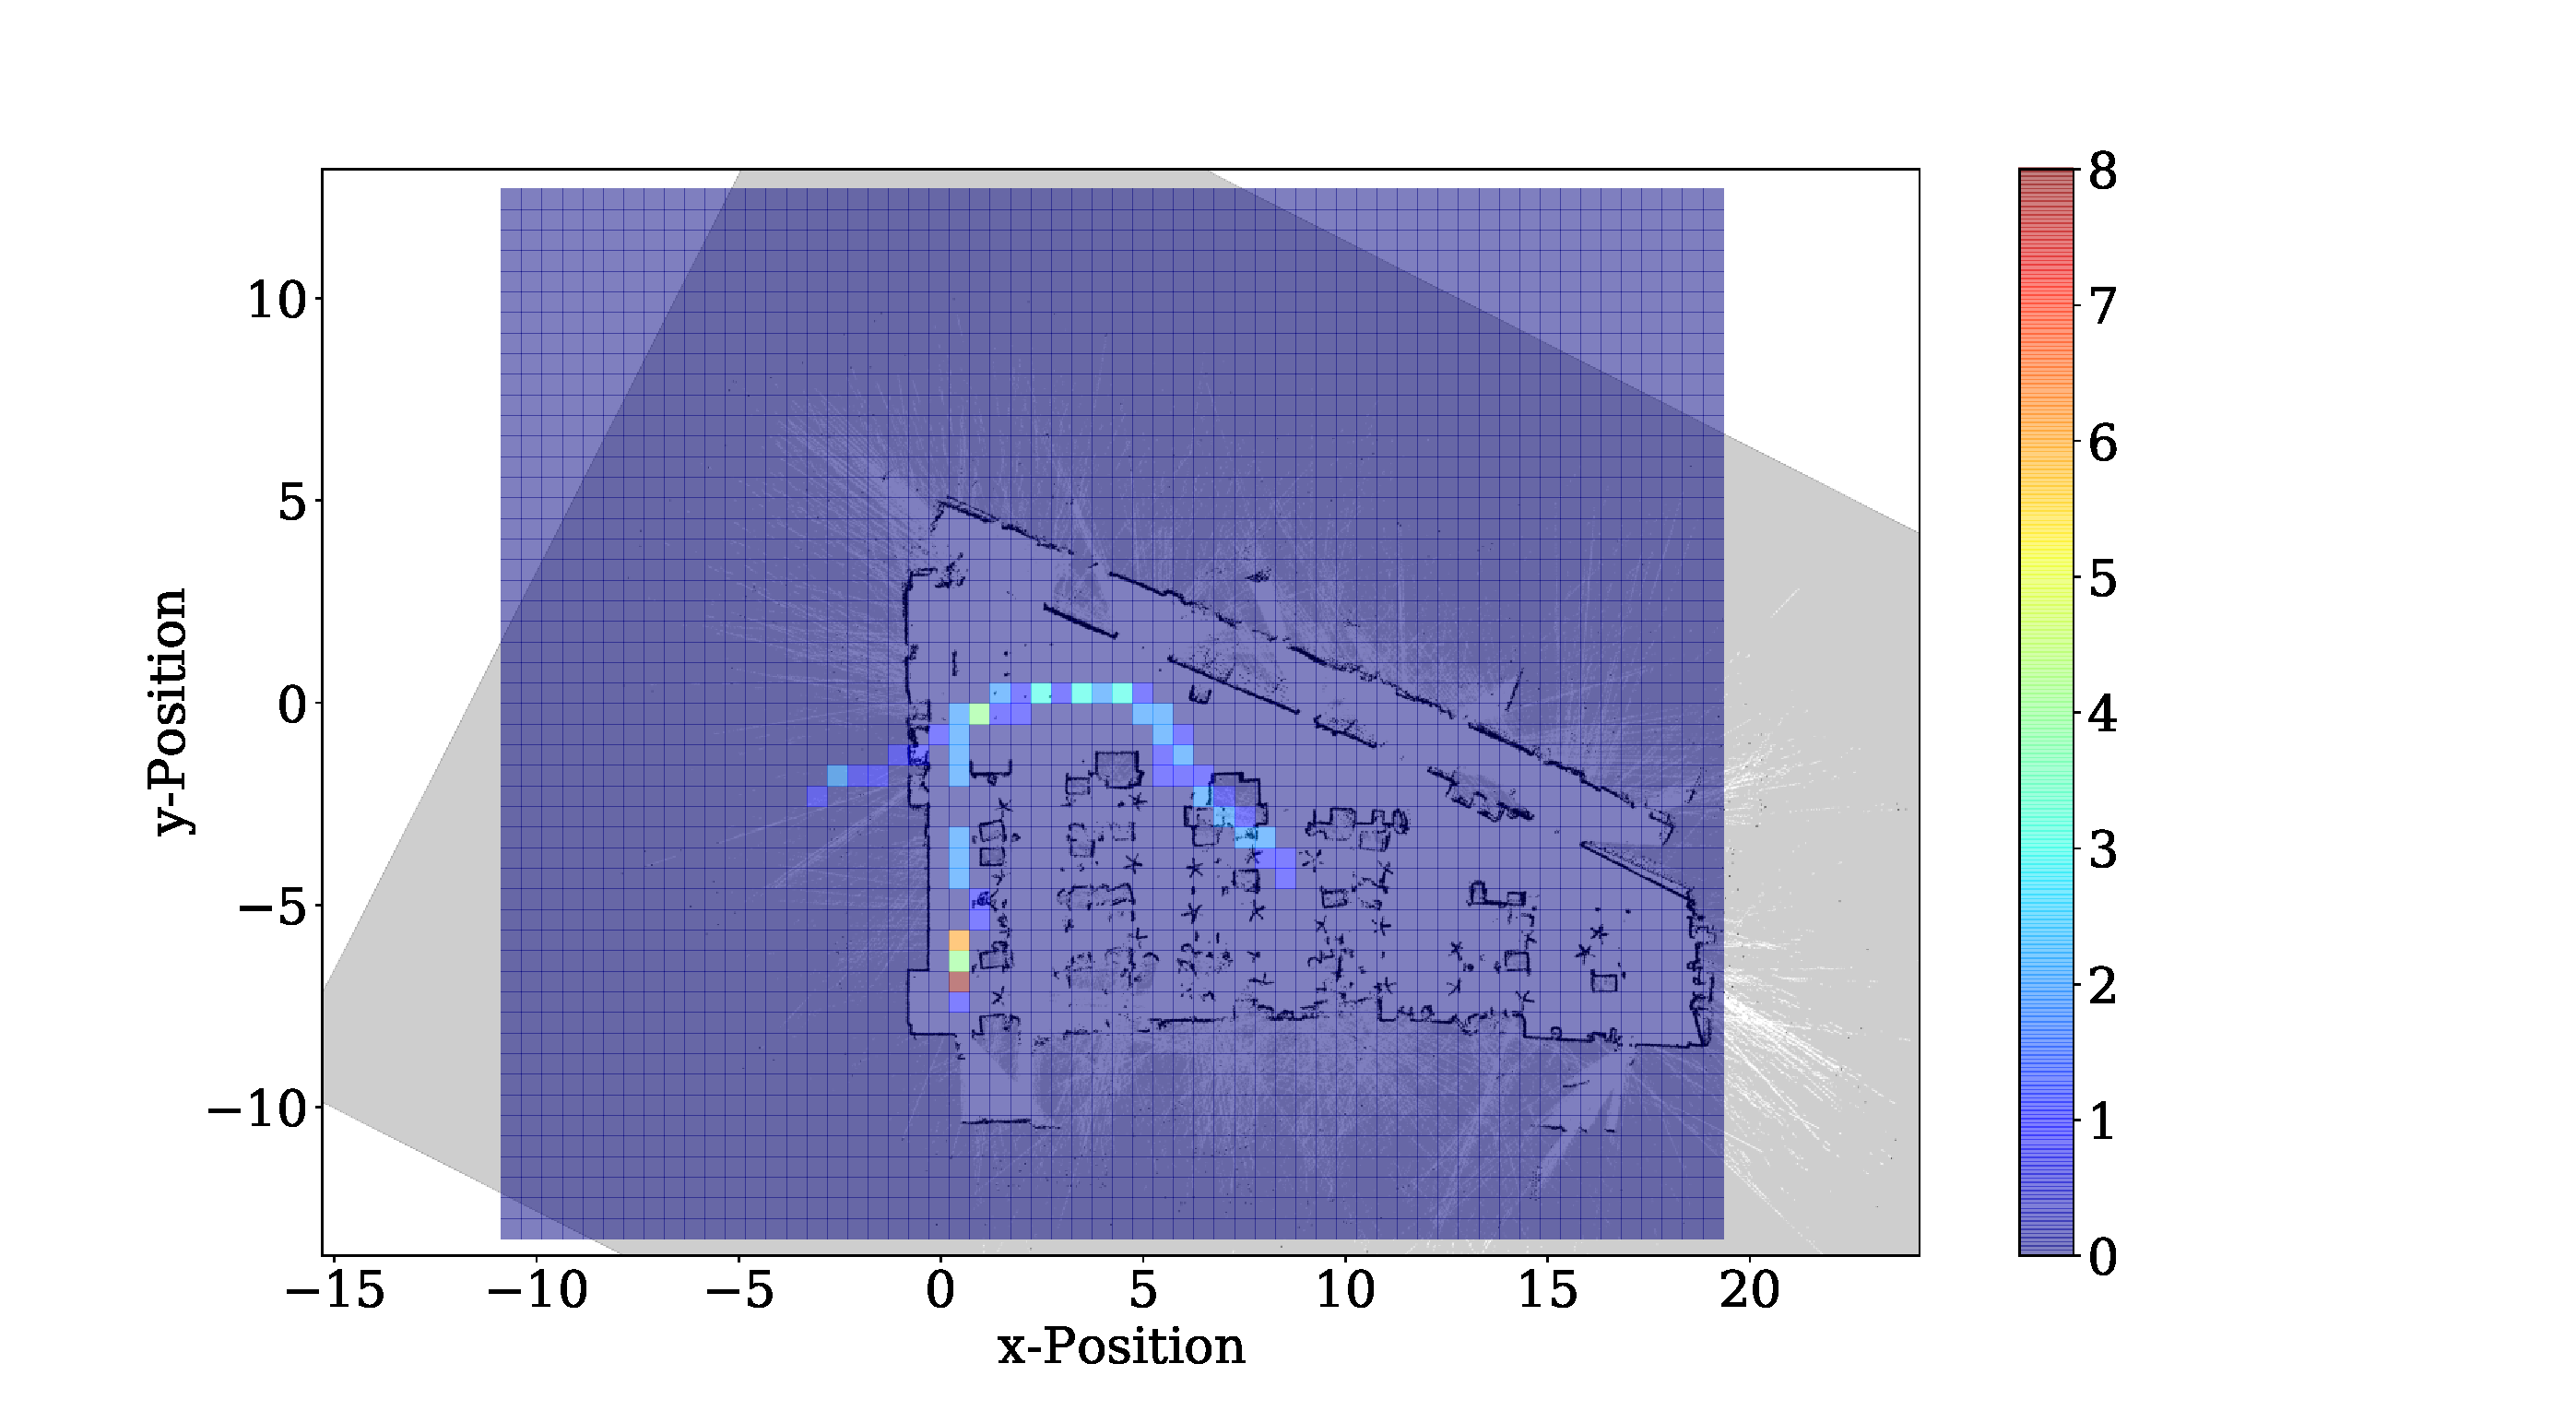
\includegraphics[width=\linewidth]{Abbildungen/methodik/Occupancy_grid_anschaulich}
		\caption[Belegungskarte grafische Darstellung]{Belegungskarte eines Bürogebäudes, über welches ein Gitter (blau) gelegt ist}
		\label{fig.Bürogebäude_Gitter}
	\end{center}
\end{figure}

Zu sehen sind hier die schematischen Umrisse eines Bürogebäudes. In blau dargestellt und über die Büroumrisse gelegt ist das oben beschriebene Gitter. Die Farbinformation spiegelt die Anzahl an Messdaten innerhalb der einzelnen Zellen wider. Eine Zelle ist dabei durch ihre x- und y-Position innerhalb des Umgebungskoordinatensystems $\textrm{(KS)}_\ind{\mathcal{U}}$ definiert. 
Ist die Umgebung $\mathcal{U}$ in einzelne Zellen unterteilt, lässt sich das oben beschriebene Gitter in Matrixschreibweise ausdrücken als
\begin{equation}
	\boldsymbol{G_\ind{Gitter}} = \begin{pmatrix}
		\boldsymbol{A}_{1,1} & \boldsymbol{A}_{1,2} &\hdots & \boldsymbol{A}_{1,n} \\
		\boldsymbol{A}_{2,1} & \boldsymbol{A}_{2,2} & \hdots & \boldsymbol{A}_{2,n} \\
		\vdots & \vdots & \ddots & \vdots \\
		\boldsymbol{A}_{n,1} & \boldsymbol{A}_{n,2} & \hdots & \boldsymbol{A}_{n,n}
	\end{pmatrix} .
\label{eq:Umgebungsmatrix}
\end{equation}

Hierbei bezeichnet $\boldsymbol{A}_{2,2}$ die Zelle der zweiten Reihe und der zweiten Spalte des Gitters, in welches die Umgebung eingeteilt wird. Es ist zu erwähnen, dass es sich um ein rechteckiges Gitter handelt, welches über die Umgebung $\mathcal{U}$ gelegt wird. Der Bereich einer Zelle $\boldsymbol{A}_{i,j}$ ist definiert durch ihre Grenzen $x_\ind{left}$ und $x_\ind{right}$ in x-Richtung, sowie die Grenzen $y_\ind{bottom}$ und $y_\ind{top}$ in y-Richtung des Umgebungskoordinatensystems $\textrm{(KS)}_\ind{\mathcal{U}}$. Eine Detektion $\boldsymbol{x}_i$ wird der Zelle $\boldsymbol{A}_{i,j}$ zugeordnet, sofern gilt 
\begin{equation}\label{eq:Grenzen einer Zelle}
	x_\ind{det} \in [x_\ind{left}, x_\ind{right}] \land y_\ind{det} \in [y_\ind{bottom}, y_\ind{top}] .
\end{equation}
Ein Eintrag in einer Zelle $\boldsymbol{A}_{i,j}$ besteht aus einem Tupel mit den Einträgen $(a, t_\ind{det})$. Der Parameter $a$ nimmt im Fall einer Personendetektion den Wert $1$ an, $t_\ind{det}$ beinhaltet die zeitliche Information der Personendetektion. Werden nach und nach mehr Detektionen innerhalb einer bestimmten Zelle getätigt, enthält die Zelle $\boldsymbol{A}_{i,j}$ eine Menge $\mathcal{L}$ bestehend aus $l$ Tupeln. Zeichnet man alle Detektionen für einen bestimmten Zeitraum, zum Beispiel für eine Woche auf, lassen sich die Messungen in Zeitintervalle $\Delta t_n$ unterteilen. Beträgt die Gesamtdauer des zum Aufzeichnen von Detektionen betrachteten Zeitraumes $T$, so ergibt sich die Gesamtzahl an Intervallen bei einer Intervalldauer von $\Delta t$ zu
\begin{equation}
	n_\ind{t} = \frac{T}{\Delta t} .
	\label{eq:Number timestamps}
\end{equation}
Die Dauer des Zeitraumes $T = t_b - t_a$ wird durch seinen Startzeitpunkt $t_a$ sowie seinen Endzeitpunkt $t_b$ definiert. Das $n$-te Zeitintervall $\Delta t_n$ befindet sich innerhalb der Grenzen $[t_a + n\Delta t,\, t_a + (n+1) \Delta t]$. Um die Übersichtlichkeit der Methodik weiterhin gewährleisten zu können, wird im Folgenden die Zelle $\boldsymbol{A}_{i,j}$ nur noch mit $\boldsymbol{A}$ bezeichnet. Um die Aktivität, beziehungsweise das Personenaufkommen in einer Zelle des Gitters bestimmen zu können, wird die Anzahl der Detektionen pro Zeitintervall aufsummiert. Die Summe an Detektionen in der Zelle $\boldsymbol{A}$ im $n$-ten Zeitintervall lässt sich schreiben als
\begin{equation}
	a_{n} = \sum_{k=1}^{K} l_k \in [t_a + n\Delta t, t_a + (n+1) \Delta t] ,
	\label{eq:Detektionen pro Intervall}
\end{equation}
wobei mit $K$ die Gesamtanzahl der Detektionen innerhalb des Gesamtzeitraumes $T$ bezeichnet wird.
Nach der Unterteilung des gesamten Zeitraumes in Intervalle und das Aufsummieren der Detektionen innerhalb dieser Intervalle enthält jede Zelle die Information des zeitlichen Verlaufes des Personenaufkommens innerhalb ihrer geografischen Grenzen. Die Zelle $\boldsymbol{A}$ und die in ihr enthaltene Information lässt sich schreiben als
\begin{equation}
	\boldsymbol{A} = (\boldsymbol{a}, \boldsymbol{t})^T .
	\label{eq:Vereinfachte Zellengleichung}
\end{equation}

Hierbei bezeichnet $\boldsymbol{a} = (a_1, a_2, \dots ,a_n)^T$ alle aufsummierten Personendetektionen innerhalb der Zeitintervalle mit den korrespondierenden Zeitstempeln $\boldsymbol{t} = (t_1, t_2, \dots ,t_n)^T$. Als Zeitstempel jeden Intervalls wird dessen Startzeitpunkt gewählt. Anschaulich beschrieben erhält man für jeden Zeitstempel die Information, wie viele Personen sich innerhalb des betreffenden Zeitintervalls in den Zellen des Gitters befunden haben. Für einen Betrachtungszeitraum mit $n$ Zeitstempeln ergibt sich eine dreidimensionale Matrix, auf dessen dritter Achse $n$ Matrizen $\boldsymbol{G}_\ind{Gitter}$ (vgl. Gleichung \ref{eq:Umgebungsmatrix}) hintereinander gestapelt werden. Im Falle des binären Zustandsmodells werden die Einträge jeder Zelle eines Zeitstempels durch die Werte $\{0,1\}$ abgebildet. Es wird lediglich das Vorhandensein einer Person innerhalb eines Zeitintervalls in einer Zelle registriert, nicht jedoch die Anzahl der Personen innerhalb des Zeitintervalls.
Ein qualitativer Vergleich der beiden Methoden kann durch \bild{occupancy_grid_vergleich} gezogen werden.

\begin{figure}[!h]
	\begin{center}
		\centering
		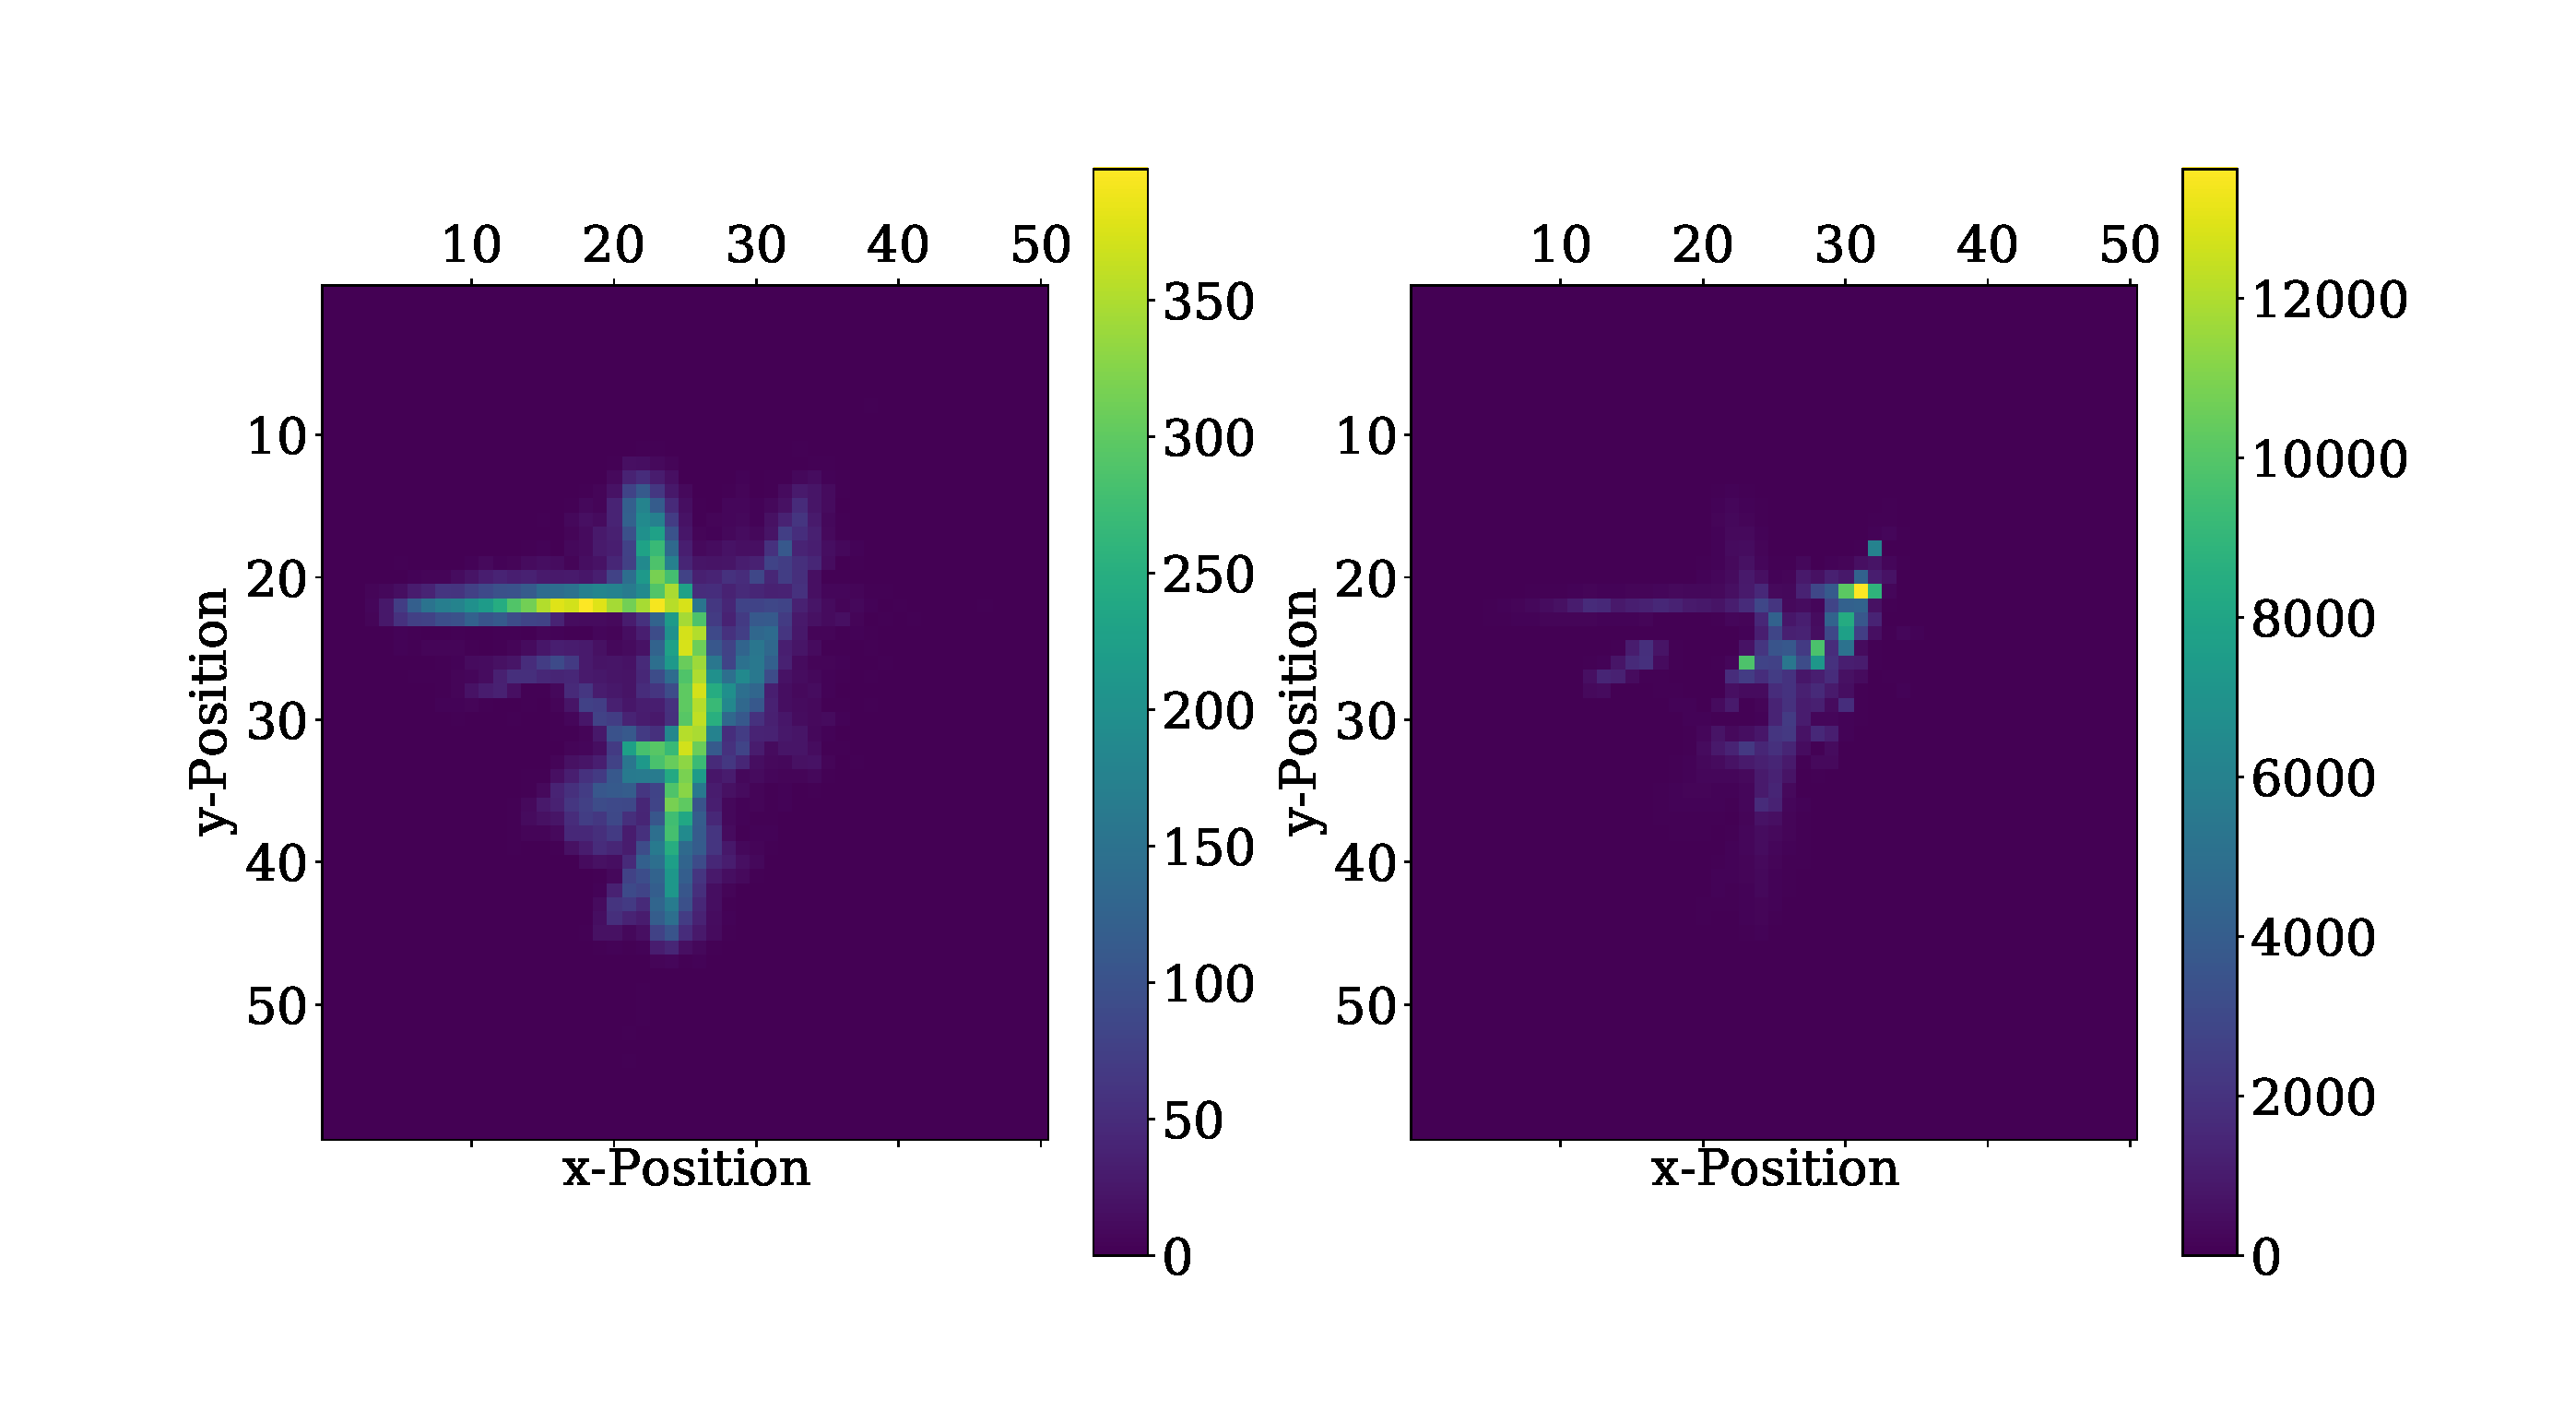
\includegraphics[width=1.0\linewidth]{Abbildungen/methodik/occupancy_grid_vergleich}
		\caption[Vergleich Personendetektion binärer und quantitativer Fall]{Aufsummierte Personendetektionen innerhalb eines Zeitraumes von einer Woche mit Beschränkung auf \{0, 1\} (links) und ohne Beschränkung (rechts)}
		\label{fig.occupancy_grid_vergleich}
	\end{center}
\end{figure}

Beiden Abbildungen liegen aufsummierte Personendetektionen innerhalb eines Zeitraumes von einer Woche mit der Aufteilung in Zeitintervalle von $\Delta t = \SI{600}{\second}$ zugrunde. Im linken Bild sieht man die Darstellung von Detektionen, welche pro Zeitintervall auf \{0,1\} beschränkt sind. Farblich hervorgehoben sind hier also Zellen, welche über viele Zeitintervalle hinweg häufig besucht wurden. Im rechten Bild dargestellt sind die nicht beschränkten, aufsummierten Personendetektionen. Farblich hervorgehoben sind hier die Zellen, welche innerhalb des gesamten Betrachtungszeitraumes am häufigsten besucht wurden, dies sich aber auf eine relativ kurze Zeitspanne innerhalb des Betrachtungszeitraumes beschränken kann. Im weiteren Verlauf dieses Kapitels wird lediglich der binäre Fall behandelt, also die auf \{0,1\} beschränkte Detektion von Personen innerhalb eines Zeitintervalls. Die so ermittelten Daten bilden einen Trend über den Betrachtungszeitraum ab. 
Die Unterteilung in Zeitintervalle ist der Tatsache geschuldet, dass in der Praxis das Wissen über die Zellzustände lückenhaft ist. Es kann lediglich durch, von einem mobilen Roboter durchgeführte, stichprobenartige Messungen approximiert werden. Mit einer größer werdenden Intervalldauer lassen sich die Messungen flexibler durchführen. Eine größere Intervalldauer geht jedoch mit einer stetig steigenden Verallgemeinerung des Zellzustandes und dem Verlust von Informationen einher. \\ 
Die registrierten Daten werden in einem weiteren Schritt in einer Datenbank gespeichert. Dies ermöglicht den externen Zugriff eines in Abschnitt \ref{sec.Verarbeitung client binär} behandelten Clients auf die Messdaten. Ein einzelner Eintrag in der Datenbank besitzt dabei immer den gleichen Aufbau. Neben dem Zellennamen werden der Zeitstempel sowie die Information, ob die Zelle im betrachteten Zeitintervall belegt oder frei war, gespeichert. 

\subsection{Verarbeitung der Messdaten Client-seitig}
\label{sec.Verarbeitung client binär}

Auf der Clientseite wird das Gitter $\boldsymbol{G}_\ind{Gitter}$ mit seinen Zelleinträgen $\boldsymbol{A}_{i,j}$ rekonstruiert. Hierzu greift der Client auf die in Abschnitt \ref{sec.Messdatenermittlung eines Belegtheitsgitters binär} beschriebene Datenbank zu und erstellt seinerseits ein Gitter, in welchem für jede Zelle eine Matrix, bestehend aus einem Vektor an Zeitstempeln und dem dazu korrespondierenden Vektor der Personendetektionen, nach Gleichung \ref{eq:Vereinfachte Zellengleichung} angelegt wird.
Der Zustand jeder einzelnen Zelle des Gitters ist als Funktion der Zeit innerhalb des Clients gespeichert und lässt sich nach \cite{Krajnik.2014} als $s(t)$ schreiben. Da auch in dieser Arbeit von dem Ansatz ausgegangen wird, dass das menschliche Verhalten, also auch das örtliche Auftreten von Personen, gewissen zeitlichen Periodizitäten unterliegt, werden die Daten der einzelnen Zellen im Folgenden an einen Server geschickt, auf welchem Untersuchungen ihrer Frequenzspektren erfolgen.

\begin{figure}[!h]
	\begin{center}
		\centering
		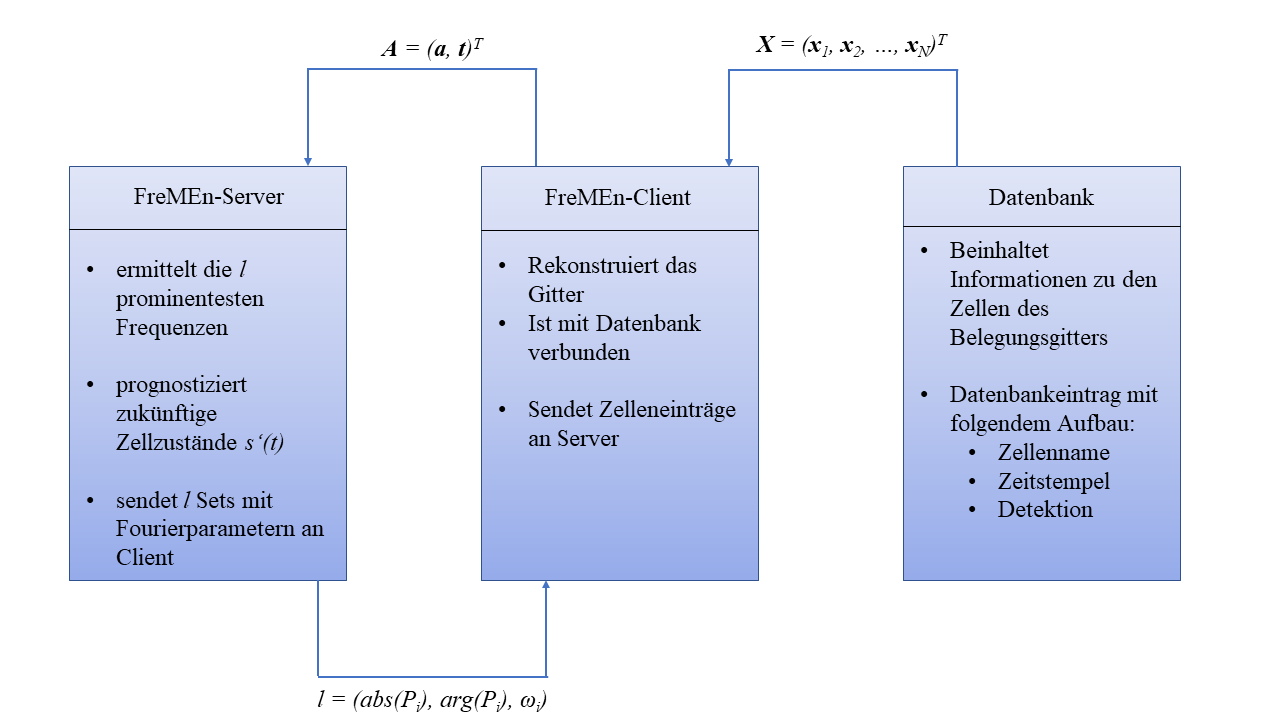
\includegraphics[width=1.0\linewidth]{Abbildungen/methodik/Ablauf_binaer}
		\caption[Informationsfluss binäres Modell]{Informationsfluss binäres Modell}
		\label{fig.Informationsfluss_binäres_Modell}
	\end{center}
\end{figure}


\subsection{Verarbeitung der Messdaten Server-seitig}
\label{sec.Verarbeitung server binär}

Der Server erstellt für jede Zelle des Belegtheitsgitters ein Modell. Als Eingang dienen dem Server die von dem Client gesendeten Datenarrays der einzelnen Zellen mit den Zeitstempeln und den dazu gehörigen Belegtheitsinformationen. Da die Zellen als linear unabhängig betrachtet werden, wird für jede Zelle ein eigenes Modell erstellt. Als Eingangsgröße dient, wie schon in \cite{Krajnik.2014}, die Belegtheit der Zelle als Funktion von der Zeit $s(t)$. Es sei darauf hingewiesen, dass $s(t)$ keine kontinuierliche, sondern eine diskrete, binäre Funktion mit Einträgen zu den Zeitpunkten der Zeitstempel ist. Die Funktion $s(t)$ soll durch eine Wahrscheinlichkeitsfunktion $p(t)$ approximiert werden. Das Vorgehen entspricht der Frequency-Map-Enhancement (FreMEn) Methode aus \cite{Krajnik.2015b}. Das Frequenzspektrum der Funktion $s(t)$ soll ermittelt werden. Hierzu wird eine inkrementelle Fouriertransformation des Zustandsvektors $s(t)$ durchgeführt mit 

\begin{equation}\label{eq:Inkrementelle Fouriertransformation} 
	\begin{split} 
		\mu &\leftarrow \frac{1}{n+1} (n \mu + s(t)) ,\\ 
		\alpha_k &\leftarrow \frac{1}{n+1} (n \alpha_k + s(t) e^{-jt \omega_k}) ,\qquad \forall \omega_k \in \Omega ,\\ 
		\beta_k &\leftarrow \frac{1}{n+1} (n \beta_k + \mu e^{-j \omega_k}) ,\qquad \quad \, \, \forall \omega_k \in \Omega ,\\ 
		n &\leftarrow n + 1 .
	\end{split} 
\end{equation} 

Gleichung \ref{eq:Inkrementelle Fouriertransformation} gleicht dem Vorgehen aus \cite{Krajnik.2015}. Mit jeder neuen Detektion werden die Werte aktualisiert. Zur Erinnerung sei darauf hingewiesen, dass die Grundidee dieser Methode darin besteht, die zeitliche Zustandsfunktion $s(t)$ jeder Zelle des Gitters durch eine Wahrscheinlichkeitsfunktion $p(t)$ zu approximieren, welcher $l$ periodische Prozesse zugrunde liegen. Die Zustandsfunktion jeder Zelle wird dabei durch die Zellzustände zu den Zeitstempeln $t_1, t_2, \dots , t_n$,\, ihren Durchschnittswert $\mu$, und zwei Mengen $\mathcal{A}, \mathcal{B}$ komplexer Zahlen $\alpha_k$ und $\beta_k$ des korrespondierenden periodischen Prozesses mit der Frequenz $\omega_k$ aus der Menge $\Omega$ beschrieben. Initialisiert wird jede Zelle mit dem Durchschnittswert $\mu = 0.5$, alle Werte $\alpha_k, \beta_k$ werden zu 0 gesetzt. Der Betrag $\gamma_k = |\alpha_k - \beta_k |$ entspricht dem durchschnittlichen Einfluss des periodischen Prozesses mit der Frequenz $\omega_k$ auf den Zellzustand $s(t)$. \\
Im Gegensatz zu \cite{Krajnik.2015} wird im Vorhinein eine feste Periodendauer $T$ von beispielsweise einer Woche vorgegeben. Da die Observationen innerhalb diskreter, über den Zeitraum $T$ gleichmäßig verteilter Intervalle $\Delta t$ erfolgen, vereinfacht sich Gleichung \ref{eq:Inkrementelle Fouriertransformation} formal zur traditionellen Diskreten Fouriertransformation (DFT). Die Informationen über den Zellzustand $s(t)$ werden, wie in Abschnitt \ref{sec.Messdatenermittlung eines Belegtheitsgitters binär} beschrieben, innerhalb einer Datenbank gespeichert. Beträgt die Gesamtdauer der in der Datenbank gespeicherten Daten $n$ mal $T$, sind also $n$ Samples der a priori definierten Periodendauer $T$ gegeben, so erfolgt eine Mittelung der Werte innerhalb korrespondierender Zeitintervalle $\Delta t_i$ durch \\

\begin{equation}\label{eq:Mittelung Fourierkoeffizienten}
	\begin{split}
		\bar{\mu} &= \frac{1}{n} \sum_{i=1}^{n} \mu_i ,	\\
		\bar{\alpha}_k &= \frac{1}{n} \sum_{i=1}^{n} \alpha_{k,i} ,\\
		\bar{\beta}_k &= \frac{1}{n} \sum_{i=1}^{n} \beta_{k,i} .
	\end{split}
\end{equation} 

Die Wahrscheinlichkeitsfunktion $p(t)$ des Zellzustandes $s(t)$ wird wie in \cite{Krajnik.2015} mittels Extraktion der $l$ periodischen Prozesse mit den höchsten Amplituden $\bar{\gamma}_k = | \bar{\alpha}_k - \bar{\beta}_k | $ gebildet. Nach deren Überlagerung ergibt sich die Wahrscheinlichkeitsfunktion $p(t)$ zu

\begin{equation}\label{eq:Zellzustands-Wahrscheinlichkeitsfunktion}
	p(t) = \zeta (\bar{\mu} + \sum_{l=1}^{m} |\bar{\gamma}_l| \cos(\omega_k t + \mathrm{arg}(\bar{\gamma}_l))) .
\end{equation}

Hierbei versichert $\zeta (.) $, dass die Funktion $p(t) \in [0, 1]$ ist. Zur Erläuterung sei angemerkt, dass, obwohl die Werte von $s(t)$ im hier betrachteten binären Fall lediglich die Zustände $\{0, 1\}$ annehmen können, die durch Fouriertransformation und inverse Fouriertransformation ermittelte Funktion $p(t)$ Werte größer als $1$ annehmen kann. \\
Die Berechnung von $p(t)$ durch Gleichung \ref{eq:Zellzustands-Wahrscheinlichkeitsfunktion} erlaubt es, zukünftige Zustände $s(t)$ einer Zelle zu ermitteln. Ein beliebiger Zeitpunkt $t$ wird dazu auf dem entsprechenden Zeitintervall $\Delta t_n$ innerhalb des Gesamtzeitraumes $T$ abgebildet. Die Vorhersage $s'(t)$ des Zellzustandes erfolgt mittels eines Schwellwertes $c$ zu

\begin{equation}\label{eq:Schwellwert-Verfahren}
	{s'}_i (t) = \begin{cases}
		1 & \, , \qquad p(t) \geq c \\
		0 & \, , \qquad p(t) < c 
	\end{cases} .
\end{equation}

Zur Ermittlung der optimalen Anzahl $l_\ind{opt}$ an periodischen Prozessen zur Bestimmung der Wahrscheinlichkeitsfunktion $p(t)$ wird auf die Einteilung des Datensatzes in ein \glqq{Estimation-Set}\grqq{} sowie ein \glqq{Prediction-Set}\grqq{} eingegangen. Ist die Gesamtdauer der in der Datenbank vorhandenen Zelleinträge $T$, so werden zur Berechnung der Modellkoeffizienten nach Gleichung \ref{eq:Inkrementelle Fouriertransformation} Daten innerhalb des Zeitintervalls $\Delta T_\ind{Est}$ verwendet. Der Schätzfehler $\epsilon_\ind{r} (T)$, also die Genauigkeit, mit der das Modell die zu seiner Erstellung verwendeten Daten rekonstruieren kann, ergibt sich zu

\begin{equation}\label{eq:Schätzfehler}
	\epsilon_\ind{r}(\Delta T_\ind{Est}) = \frac{1}{n} \sum_{i=1}^{n} |s_i '(t) - s_i (t)| .
\end{equation}

Alle zur Berechnung des Fehlers $\epsilon_\ind{r}$ verwendeten Daten müssen innerhalb des Intervalls $\Delta T_\ind{Est}$ liegen. \\
Das Zeitintervall $\Delta T_\ind{Pred}$ beinhaltet Messungen, welche nicht zur Erstellung des Modells verwendet wurden. Der Fehler $\epsilon_\ind{p}$ beschreibt, wie genau das Modell zukünftige Zustände einer Zelle vorhersagen kann. Der Fehler $\epsilon_\ind{p}$ berechnet sich als

\begin{equation}
	\label{eq:Prädiktionsfehler}
		\epsilon_\ind{p}(\Delta T_\ind{Pred}) = \frac{1}{n} \sum_{i=1}^{n} |s_i '(t) - s_i (t)| ,
	\end{equation}
	
mit allen Messwerten innerhalb des Intervalls $\Delta T_\ind{Pred}$. Die optimale Modellordnung $l_\ind{opt}$ wird nach \cite{Krajnik.2015} so gewählt, dass der Prädiktionsfehler $\epsilon_\ind{p}$ minimiert wird. Die maximale Modellordnung wird zu $l_\ind{max} = 20$ gesetzt. \\

\section{Quantitative Zustandsmodelle}
\label{sec.Quantitative Zustandsmodelle}
Um Aussagen über die Anzahl an Ereignissen innerhalb eines Zeitintervalls treffen zu können, kann dies, wie schon in Abschnitt \ref{sec.Beschreibung quantitativer Zustandsmodelle} erwähnt, mittels quantitativer Zustandsmodelle erreicht werden. Es sollen Schätzungen $\lambda'(t)$ für die, intervallweise definierte, Funktion $\lambda(t)$ einer Aktivitätenrate berechnet werden. Hierzu folgt in einem ersten Schritt die Ermittlung von Messdaten eines Belegtheitsgitters (Abschnitt \ref{sec.Messdatenermittlung quantitativ}), bevor diese Daten Client-seitig verarbeitet werden (Abschnitt \ref{sec.Messdatenverarbeitung client quantitativ}). In einem weiteren Schritt werden die Daten an einen Server gesendet, welcher für jede Zelle des Belegtheitsgitters ein quantitatives Zustandsmodell erstellt (Abschnitt \ref{sec.Messdatenverarbeitung server quantitativ}).
\subsection{Messdatenermittlung eines Belegtheitsgitters}
\label{sec.Messdatenermittlung quantitativ}

Wie schon in Abschnitt \ref{sec.Binäre Zustandsmodelle} wird auch in diesem Abschnitt, welcher quantitative Zustandsmodelle behandelt, ein Gitter über eine Umgebung $\mathcal{U}$ gelegt, und für einen Betrachtungszeitraum $T$, unterteilt in $n$ Intervalle mit der Intervalldauer $\Delta t$, die Personendetektionen innerhalb der Zellen gezählt. Die Methodik gleicht der des binären Modells, jedoch erfolgt keine Beschränkung der Detektionen pro Intervall auf \{0,1\}. Die Einträge einer einzelnen Zelle des Gitters werden geschrieben als
\begin{equation}
	\boldsymbol{A} = (\boldsymbol{\lambda}, \boldsymbol{t})^T .
	\label{eq:Zelleinträge quantitativer Fall}
\end{equation}

Da im quantitativen Fall die Anzahl an Personen pro Zeitintervall $\Delta t$, also die Personenrate gezählt wird, enthält Gleichung \ref{eq:Zelleinträge quantitativer Fall} die Personenraten $\boldsymbol{\lambda} = (\lambda_1, \lambda_2, \dots , \lambda_n)^T$ \, der einzelnen Zeitintervalle sowie die Zeitstempel $\boldsymbol{t} = (t_1, t_2, \dots , t_n)^T$ \, der zugehörigen Intervalle. Eine Erhöhung der Intervalldauer $\Delta t$ geht dabei mit steigenden Einträgen der Personenraten $\boldsymbol{\lambda}$ und einem Informationsverlust einher. \\
Die registrierten Daten werden, wie schon in Abschnitt \ref{sec.Messdatenermittlung eines Belegtheitsgitters binär}, in einer Datenbank gespeichert. Ein Datenbankeintrag enthält neben dem Zellennamen den Zeitstempel des Zeitintervalls sowie die zugehörige Personenrate $\lambda$.

\subsection{Verarbeitung der Messdaten Client-seitig}
\label{sec.Messdatenverarbeitung client quantitativ}

Die Verarbeitung der Messdaten auf der Clientseite gleicht dem Vorgehen in Abschnitt \ref{sec.Verarbeitung client binär}. Das Gitter $\boldsymbol{G}_\ind{Gitter}$ mit seinen Zelleinträgen $\boldsymbol{A}_{i,j}$ wird rekonstruiert. Jede rekonstruierte Zelle enthält einen Vektor $\boldsymbol{t}$ an Zeitstempeln und den Vektor $\boldsymbol{\lambda}$ der Personenraten der einzelnen Zeitintervalle. Die beiden Vektoren jeder Zelle werden im nächsten Schritt an den Server geschickt, auf welchem Untersuchungen der Frequenzspektren der Zelle erfolgen.

\begin{figure}[!h]
	\begin{center}
		\centering
		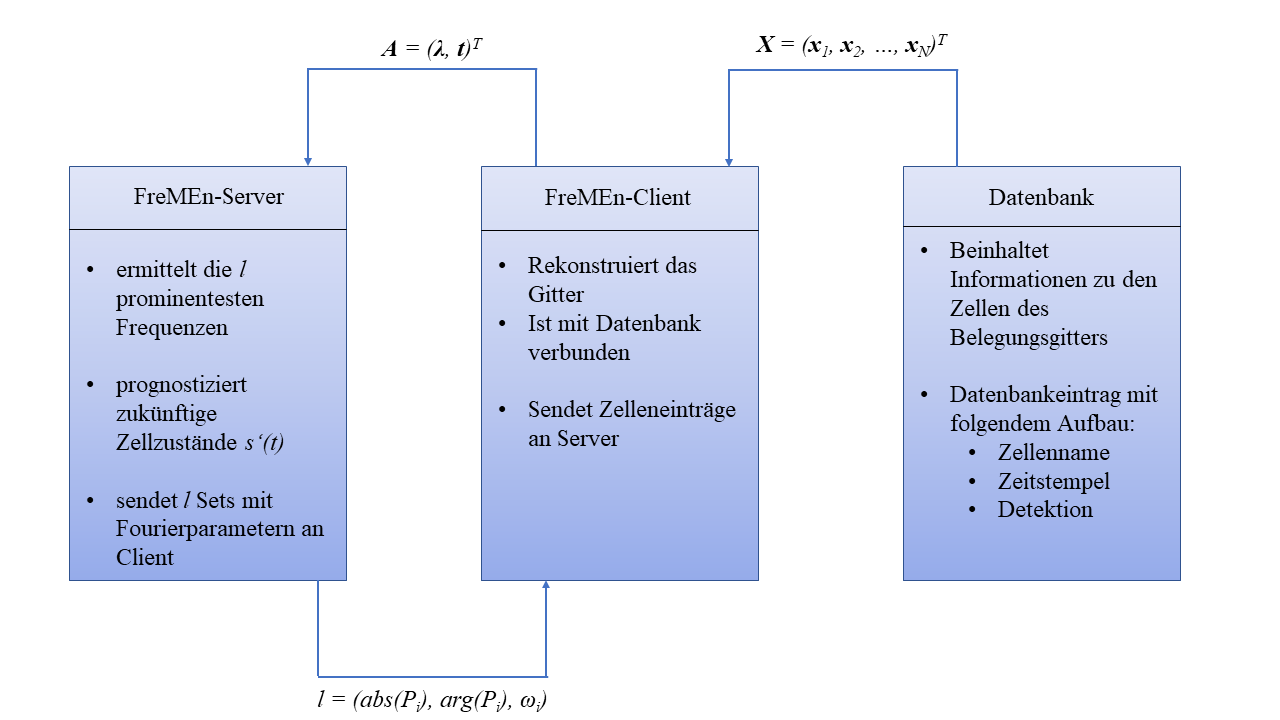
\includegraphics[width=1.0\linewidth]{Abbildungen/methodik/Ablauf_quantitativ}
		\caption[Informationsfluss quantitatives Modell]{Informationsfluss quantitatives Modell}
		\label{fig.Informationsfluss_quantitatives_Modell}
	\end{center}
\end{figure}

\subsection{Verarbeitung der Messdaten Server-seitig}
\label{sec.Messdatenverarbeitung server quantitativ}

Wie schon in Abschnitt \ref{sec.Verarbeitung client binär} erstellt der Server auch für den quantitativen Fall für jede Zelle des Belegtheitsgitters ein Modell. Wieder wird aufgrund der linearen Unabhängigkeit der Zellen für jede einzelne Zelle ein eigenes Modell erstellt. Als Eingangsgröße dient, wie in \cite{Jovan.2016}, die Personenrate $\lambda (t)$ als Funktion der Personenraten der einzelnen Zeitintervalle $\Delta t$. Die Funktion $\lambda (t)$ soll durch eine Funktion $\lambda ' (t)$ approximiert werden. Nach \cite{Krajnik.2015b} erfolgt eine inkrementelle Fouriertransformation der Personenraten-Funktion $\lambda (t)$ durch Gleichung \ref{eq:Inkrementelle Fouriertransformation}. Liegen in der Datenbank insgesamt $n$ Samples der a priori definierten Periodendauer $T$ vor, so erfolgt eine Mittelung der Werte korrespondierender Zeitintervalle $\Delta t_i$ nach Gleichung (\ref{eq:Mittelung Fourierkoeffizienten}). Die Approximation $\lambda ' (t)$ der Personenraten-Funktion $\lambda (t)$ ergibt sich zu
\begin{equation}\label{eq:Personenraten-Funktion}
	\lambda ' (t) = \zeta (\bar{\mu} + \sum_{l=1}^{m} |\bar{\gamma}_l| \cos(\omega_k t + \mathrm{arg}(\bar{\gamma}_l))) .
\end{equation} 

Hierbei versichert $\zeta (.) $, dass die Funktion $\lambda ' (t)$  den  Wert der am nächsten liegenden, natürlichen Zahl, annimmt. 
Zur Ermittlung der optimalen Anzahl $l_\ind{opt}$ an periodischen Prozessen zur Bestimmung der Personenraten-Funktion $\lambda (t)$ wird der Datensatz in ein \glqq{Estimation-Set}\grqq{} sowie ein \glqq{Prediction-Set}\grqq{} eingeteilt. Der Schätzfehler $\epsilon_\ind{r} (T)$, also die Genauigkeit, mit der das Modell die zu seiner Erstellung verwendeten Daten rekonstruieren kann, berechnet sich durch
\begin{equation}\label{eq:Schätzfehler quantitativ}
	\epsilon_\ind{r}(\Delta T_\ind{Est}) = \frac{1}{n} \sum_{i=1}^{n} |\lambda_i '(t) - \lambda_i (t)| .
\end{equation}
Alle zur Berechnung des Fehlers $\epsilon_\ind{r}$ verwendeten Daten müssen innerhalb des Intervalls $\Delta T_\ind{Est}$ liegen. \\
Das Zeitintervall $\Delta T_\ind{Pred}$ beinhaltet Messungen, welche nicht zur Erstellung des Modells verwendet wurden. Somit beschreibt der Fehler $\epsilon_\ind{p}$ wie schon in Abschnitt \ref{sec.Messdatenverarbeitung server quantitativ}, wie genau das Modell zukünftige Personenraten einer Zelle vorhersagen kann. Der Fehler $\epsilon_\ind{p}$ beträgt
\begin{equation}\label{eq:Prädiktionsfehler quantitativ}
	\epsilon_\ind{p}(\Delta T_\ind{Pred}) = \frac{1}{n} \sum_{i=1}^{n} |\lambda_i '(t) - \lambda_i (t)| ,
\end{equation}
mit allen Messwerten innerhalb des Intervalls $\Delta T_\ind{Pred}$. Die optimale Modellordnung $l_\ind{opt}$ wird so gewählt, dass der Prädiktionsfehler $\epsilon_\ind{p}$ minimiert wird. Die maximale Modellordnung wird zu $l_\ind{max} = 20$ gesetzt.
    	\chapter{Evaluation}
\label{sec.Evaluation}
Dieses Kapitel behandelt die Evaluation der nach den in Kapitel \ref{sec.Methodik} beschriebenen Schritten erstellten binären und quantitativen Modellen. In einem ersten Schritt werden die zur Modellerstellung benutzten Datensätze vorgestellt (Abschnitt \ref{sec.Datensätze}). Darauf aufbauend erfolgt eine Einführung der Fehlermaße (Abschnitt \ref{sec.Beschreibung der Fehlermaße}) für das binäre sowie das quantitative Modell, mit denen die Prädiktionsgenauigkeiten beider Modelle bewertet werden können. Die Bewertung der Modelle erfolgt separat für den binären Fall (Abschnitt \ref{sec.Binäres Modell}) und den quantitativen Fall (Abschnitt \ref{sec.Quantitatives Modell}). Es werden Vergleiche der Modelle gegenüber statischen Repräsentationen von Personen-Auftrittswahrscheinlichkeiten (binäres Modell) sowie Personenraten (quantitatives Modell) gezogen. Im Rahmen dieser Vergleiche werden außerdem limitierende Modellfaktoren erörtert. \\
\section{Datensätze}
\label{sec.Datensätze}
Zur Evaluation der in dieser Arbeit präsentierten Methoden dienen zwei separate Datensätze. Für den im Folgenden als  \glqq Aruba-Datensatz\grqq{} bezeichneten Datensatz wurde über einen Zeitraum von 16 Wochen das Personenaufkommen innerhalb einer Wohnung aufgezeichnet \cite{aruba}. Hierbei wurde die Wohnung in insgesamt zehn verschiedene Räume aufgeteilt und minütlich der Aufenthaltsort einer Person dokumentiert. Als Beschränkung gilt, dass sich zu jedem Zeitpunkt nur maximal eine Person in der Wohnung befinden konnte. Befand sich die Person außerhalb der Wohnung, so ist dies im Datensatz als Raum \glqq Outside\grqq{} dokumentiert.
Die in den folgenden Abschnitten durchgeführten Untersuchungen beruhen stets auf einem Modell, welches mittels der Daten der ersten zwölf der insgesamt 16 Wochen nach den Gleichungen \ref{eq:Inkrementelle Fouriertransformation} trainiert wurde. Jeder der zehn Räume ist dabei durch eine einzelne Zelle repräsentiert. Zur Evaluation des Modells wird der Prädiktionsfehler $\epsilon_\ind{p}$ für die letzten vier Wochen des Datensatzes berechnet. Als Modellordnung $l_\ind{opt}$ wird, wie schon in Abschnitt \ref{sec.Verarbeitung server binär} beschrieben, die Ordnung mit dem geringsten Prädiktionsfehler $\epsilon_\ind{p,opt}$ gewählt.  \\
% Hier die Quelle von dem Datensatz einfügen?
Der zweite Datensatz, im Folgenden als \glqq {UOL-Datensatz}\grqq{} bezeichnet, wurde durch einen, an einer statischen Position befindlichen, 3D-Laserscanner innerhalb eines Bürokomplexes des Isaac Newton Building der University of Lincoln (UOL) aufgenommen \cite{uol}. Über einen Zeitraum von 22 aufeinanderfolgenden Tagen, beginnend mit dem 23. November 2018, wurden mit einer Frequenz von $\SI{0.5}{\hertz}$ Personendetektionen mit den zugehörigen Zeitstempeln und Positionsdaten innerhalb einer Umgebung mit einer Gesamtfläche von ca. \SI{85}{\metre\squared} aufgezeichnet \cite{uol}. Zur Modellberechnung in den folgenden Abschnitten wird über das Bürogebäude ein Gitter mit den Maßen $\SI{30}{\metre} \, \mathrm{x} \, \SI{25.5}{\metre}$ gelegt. Jede Zelle innerhalb des Gitters hat die Maße $\SI{0.5}{\metre} \, \mathrm{x} \, \SI{0.5}{\metre}$, sodass man insgesamt 3060 verschiedene Zellen erhält. Die ersten zwei Wochen des Datensatzes werden für die Erstellung des Modells verwendet. Zur Evaluierung wird $\epsilon_\ind{p}$ mittels der Daten der dritten Woche berechnet. Als Modellordnung wird auch hier die Ordnung $l_\ind{opt}$ mit dem geringsten Prädiktionsfehler $\epsilon_\ind{p,opt}$ gewählt. 

\section{Beschreibung der Fehlermaße}
\label{sec.Beschreibung der Fehlermaße}
Um die Prädiktionsgenauigkeit der Modelle bewerten zu können, ist ein einheitliches Fehlermaß notwendig. Im Folgenden werden daher sowohl für das binäre wie auch für das quantitative Modell Fehlermaße eingeführt, welche in einem späteren Abschnitt dieses Kapitels für Vergleiche mit statischen Modellen herangezogen werden.
\subsection{Fehlermaße des binären Modells}
\label{sec.Fehlermaße binäres Modell}
Für die Bewertung der Modelle wird ein einheitliches Fehlermaß benutzt. Wie schon in Abschnitt \ref{sec.Beschreibung binärer Zustandsmodelle} beschrieben und auch in \cite{Krajnik.2014} erwähnt, führt eine Erhöhung der Modellordnung dazu, dass die zur Erstellung des Modells verwendeten Daten besser abgebildet werden können. Der Rekonstruktionsfehler $\epsilon_\ind{r}$ sinkt. Der Einfluss auf den Prädiktionsfehler $\epsilon_\ind{p}$, also die Genauigkeit, mit der zukünftige Zellzustände modelliert werden können, ist jedoch komplexer.
Grafisch dargestellt ist dies in \bild{prediction_vs_estimation_error}.
% Achsbeschriftungen in Prozent umschreiben
\begin{figure}[!h]
	\centering
	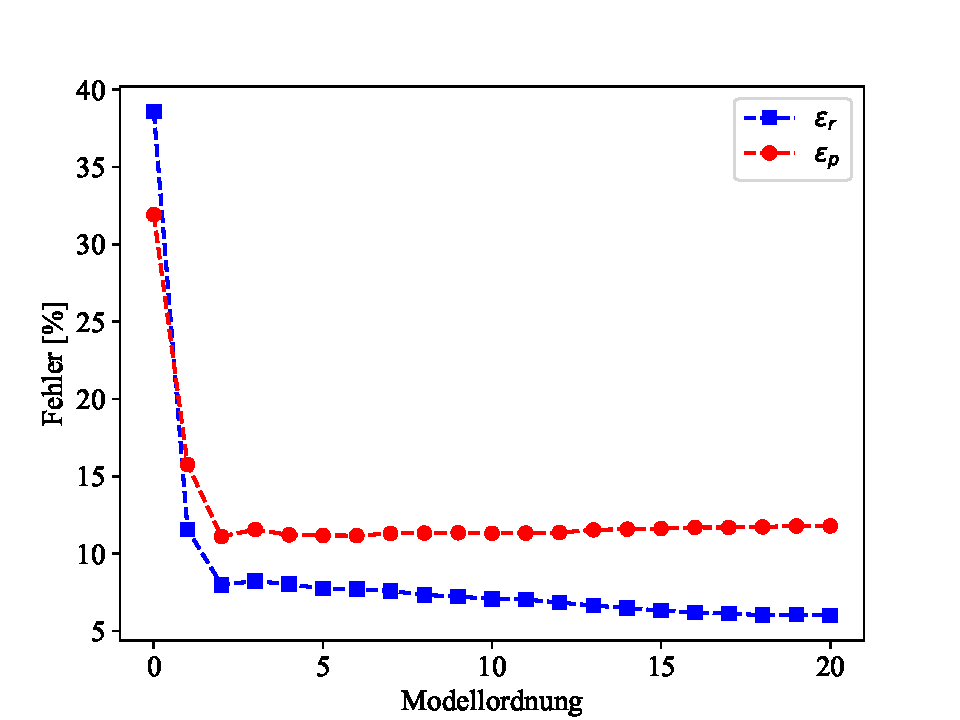
\includegraphics[width=0.7\linewidth]{Abbildungen/evaluation/prediction_vs_estimation_error}
	\caption{Rekonstruktionsfehler $\epsilon_\ind{r}$ und Prädiktionsfehler $\epsilon_\ind{p}$ mit steigender Modellordnung}
	\label{fig.prediction_vs_estimation_error}
\end{figure}

Zur Bewertung der Modellgenauigkeiten wird in den folgenden Abschnitten stets die Modellordnung $l_\ind{opt}$ mit dem geringsten Prädiktionsfehler $\epsilon_\ind{p,opt}$ gewählt. Der Fehler berechnet sich dabei nach Gleichung \ref{eq:Prädiktionsfehler}. Die maximale Modellordnung wird zu $l_\ind{max} = 20$ gesetzt. Der Schwellwert zur Ermittlung des prognostizierten Zellzustandes $s'(t)$ mittels der Zellwahrscheinlichkeitsfunktion $p(t)$ beträgt $c = 0.5$ (siehe Gleichung \ref{eq:Schwellwert-Verfahren}).

\subsection{Fehlermaße quantitatives Modell}
\label{sec.Fehlermaße quantitatives Modell}
Die optimale Modellordnung $l_\ind{opt}$ des quantitativen Modells berechnet sich ebenfalls durch die Minimierung des Prädiktionsfehlers $\epsilon_\ind{p}$. Da für den quantitativen Fall jedoch die Personenraten $\lambda' (t)$ für die einzelnen Intervalle $\Delta t_i$ berechnet werden, erfolgt die Ermittlung des Prädiktionsfehlers nach Gleichung \ref{eq:Prädiktionsfehler quantitativ}.
% In Kapitel Methodik noch die Berechnung vom Prädiktionsfehler nach lsme-Methode reinschreiben.
Die Rate $\lambda ' (t)$ wird auf die nächste natürliche Zahl gerundet, damit sichergestellt ist, dass $\lambda ' (t) \in \mathbb{N}$ gilt. Die maximale Modellordnung wird zu $l_\ind{max} = 20$ gesetzt.
\section{Binäres Modell}
\label{sec.Binäres Modell}
In diesem Abschnitt erfolgt eine Evaluation des binären Modells. Untersucht wird das Modell bei unterschiedlichen Intervalldauern $\Delta t$. Für den binären Fall berechnen sich die Personendetektionen im $n$-ten Zeitintervall (siehe Gleichung \ref{eq:Detektionen pro Intervall}) zu

\begin{equation}\label{eq:Fallunterscheidung a_n}
	a_n = \begin{cases}
		1 & , \qquad a_n \geq 1 \\
		0 & , \qquad a_n < 1 \, 
	\end{cases} .
\end{equation}

Die Einteilung der gesamten Periodendauer, wie beispielsweise einer Woche, in unterschiedlich lange Intervalldauern, resultiert aus der Tatsache, dass ein mobiler Roboter im Normalfall keine komplette Übersicht über die zu modellierende Umgebung $\mathcal{U}$ besitzt. Mit einer Vergrößerung der Intervalldauer soll sichergestellt werden, dass der Roboter innerhalb dieser Dauer die Umgebung $\mathcal{U}$ mindestens einmal komplett abfahren kann. Begründet werden kann dies damit, dass im vorliegenden Modell das Nicht-Beobachten einer Zelle einer Nicht-Detektion von Personen entspricht. Wird während eines Intervalls mindestens eine Person detektiert, so wird der Zellenstatus im entsprechenden Intervall auf $s(t) = 1$ gesetzt. Die Dauer des Aufenthaltes des Roboters in einer Zelle innerhalb eines Intervalls kann nicht berücksichtigt werden. Je nach Umgebungsgröße und Detektionsbereich des mobilen Roboters sollte die Intervalldauer angepasst werden. Die Summe an Zeitstempeln innerhalb der Periodendauer reduziert sich mit steigender Intervalldauer $\Delta t$ und geht somit mit einem Informationsverlust einher. Der Zellzustand $s(t)$ bei unterschiedlichen Intervalldauern $\Delta t$ ist in \bild{bin_size_influence_master_bedroom_binary} dargestellt. 


\begin{figure}[!h]
		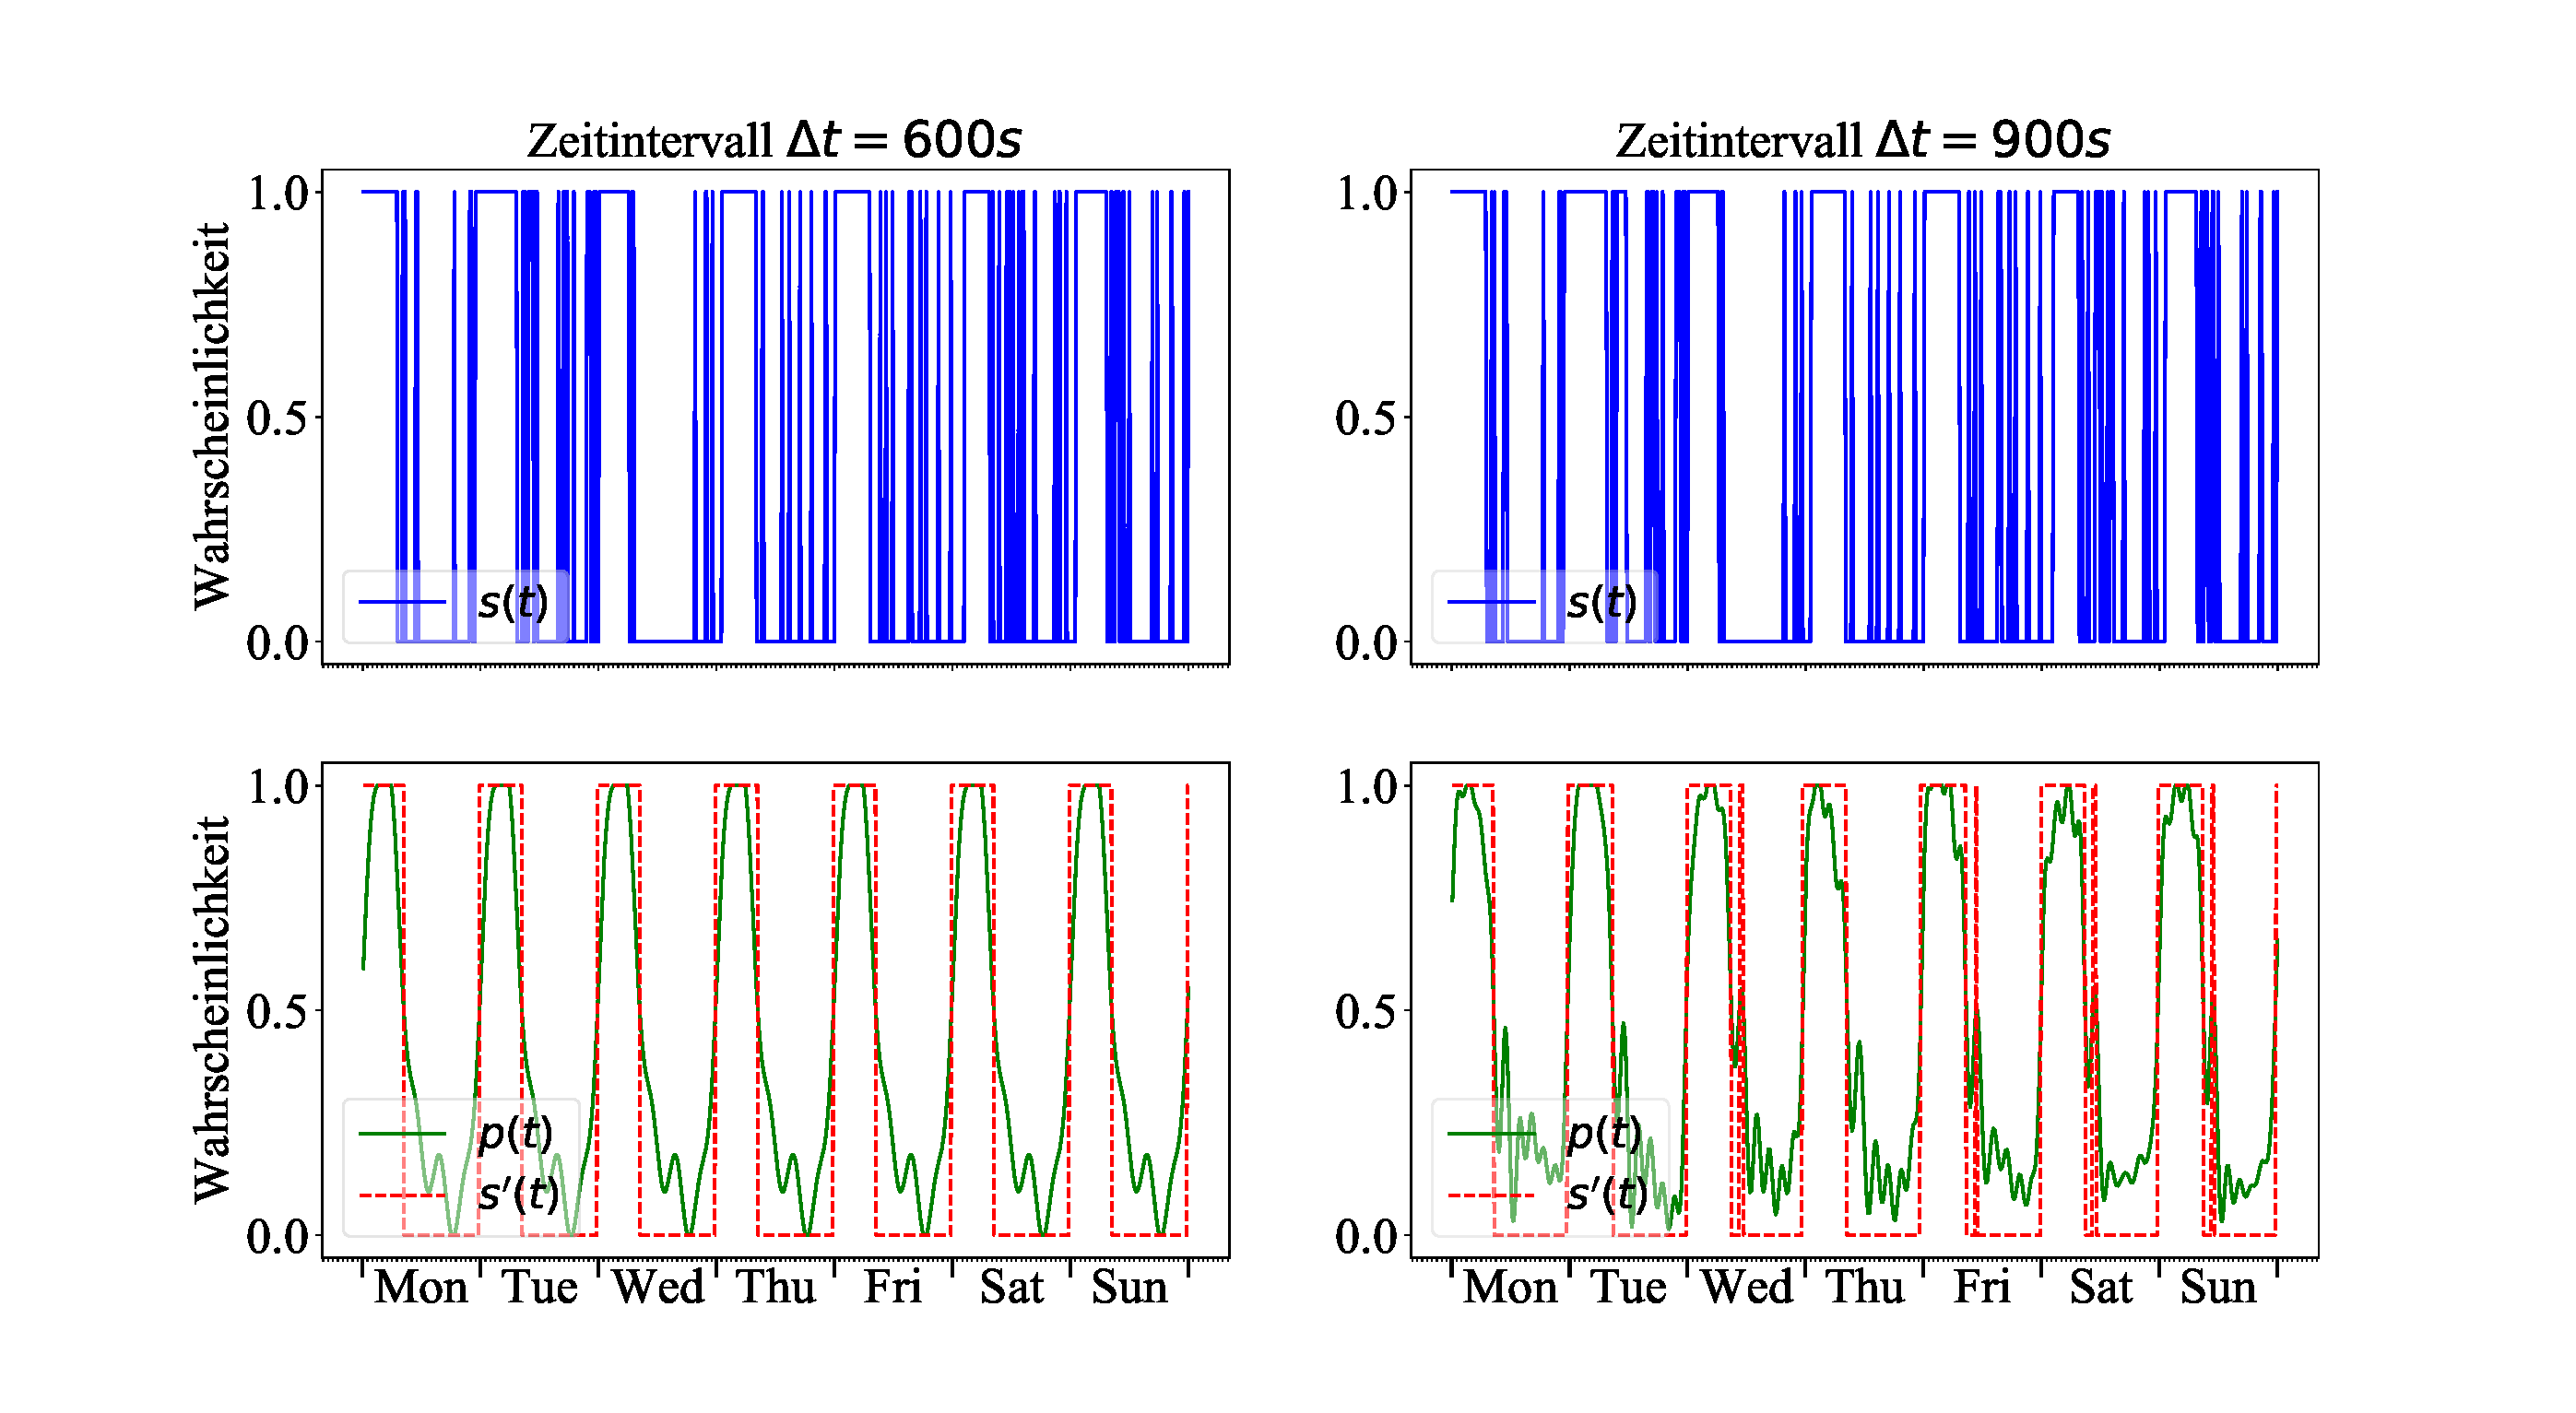
\includegraphics[width=\linewidth]{Abbildungen/evaluation/bin_size_influence_master_bedroom_binary.pdf}
		\caption[Zellzustand $s(t)$ sowie Wahrscheinlichkeitsfunktion $p(t)$ und prognostizierter Zellzustand $s'(t)$ des Schlafzimmers des Apartments mit einer Intervalldauer von $\Delta t = \SI{600}{\second}$ und $\Delta t = \SI{900}{\second}$]{Zellzustand $s(t)$ sowie Wahrscheinlichkeitsfunktion $p(t)$ und prognostizierter Zellzustand $s'(t)$ des Schlafzimmers des Apartments (Aruba-Datensatz) mit einer Intervalldauer von $\Delta t = \SI{600}{\second}$ (links) und $\Delta t = \SI{900}{\second}$ (rechts)}
		\label{fig.bin_size_influence_master_bedroom_binary}
\end{figure}

% Hier Abbildung einfügen von Master-Bedroom
Betrachtet wird hier das Schlafzimmer des Apartments des Aruba-Datensatzes. 
Die beiden Grafiken auf der linken Seite zeigen den Zellzustand $s(t)$ (oben) über einen Gesamtzeitraum von einer Woche für eine Intervalldauer von $\Delta t = \SI{600}{\second} $, die Wahrscheinlichkeitsfunktion $p(t)$ der Zelle sowie der anhand des Schwellwertes $c = 0.5$  prognostizierte Zellzustand $s'(t)$. Auf der rechten Seite von \bild{bin_size_influence_master_bedroom_binary} ist der Zellzustand $s(t)$ für eine Intervalldauer von $\Delta t = \SI{900}{\second}$ sowie die Wahrscheinlichkeitsfunktion der Zelle und der prognostizierte Zellzustand $s'(t)$ aufgetragen. Während zur Bestimmung von $p(t)$ im Falle von $\Delta t = \SI{600}{\second} $ eine Modellordnung von $l_\ind{opt} =2$ einen Prädiktionsfehler von $\epsilon_\ind{p,opt} = 17.8 \% $ erreicht,
beträgt die optimale Modellordnung $l_\ind{opt} =3$ bei einer Intervalldauer von $\Delta t = \SI{900}{\second}$  mit einem Prädiktionsfehler  von $\epsilon_\ind{p,opt} = 7.4 \% $. Hierbei ist anzumerken, dass aus den obigen Ergebnissen nicht geschlossen werden kann, dass eine Intervalldauer von $\Delta t = \SI{900}{\second}$ ein genaueres Modell erzeugt als eine Intervalldauer von $\Delta t = \SI{600}{\second}$. Die Ergebnisse der unterschiedlichen Intervalle sind nicht miteinander vergleichbar. Eine höhere Intervalldauer geht mit einer größeren Wahrscheinlichkeit mindestens einer Personendetektion einher. Somit steigt der Anteil an Intervallen, in denen Personendetektionen vorliegen, gegenüber der Gesamtanzahl an Zeitintervallen. Wie bereits am Anfang dieses Abschnittes erwähnt, geht eine Vergrößerung der Intervalldauer $\Delta t$ immer auch mit einem Informationsverlust einher. Eine Bewertung der Modelle kann jedoch durch den Vergleich mit den zugehörigen statischen Modellen gezogen werden.  Für den statischen Fall, also die Annahme einer konstanten Wahrscheinlichkeit $p_\ind{stat}(t) = \mathrm{const}.\, $, ergibt sich $\epsilon_\ind{p,stat} = 40.5 \%$ für eine Intervalldauer von $\Delta t = \SI{600}{\second}$, der statische Prädiktionsfehler bei einer Intervalldauer von $\Delta t = \SI{900}{\second}$ berechnet sich zu $\epsilon_\ind{p,stat} = 44.3 \%$. Die größere Intervalldauer spiegelt sich in dem Modell derart wider, dass die Anzahl der Personendetektionen im Verhältnis zu der Anzahl $n$ der Zeitstempel zunimmt, und die Breite der rot gestrichelten Balken, welche Phasen einer durchgängigen Zellbelegtheit signalisieren, in \bild{bin_size_influence_master_bedroom_binary} zunimmt.\\
Eine Limitation der Methode ist jedoch in \bild{bin_size_influence_second_bedroom_binary} zu sehen. Betrachtet wird der Zellzustand $s(t)$ des Gästeschlafzimmers innerhalb des Apartments.

\begin{figure}[!h]
	\begin{center}
		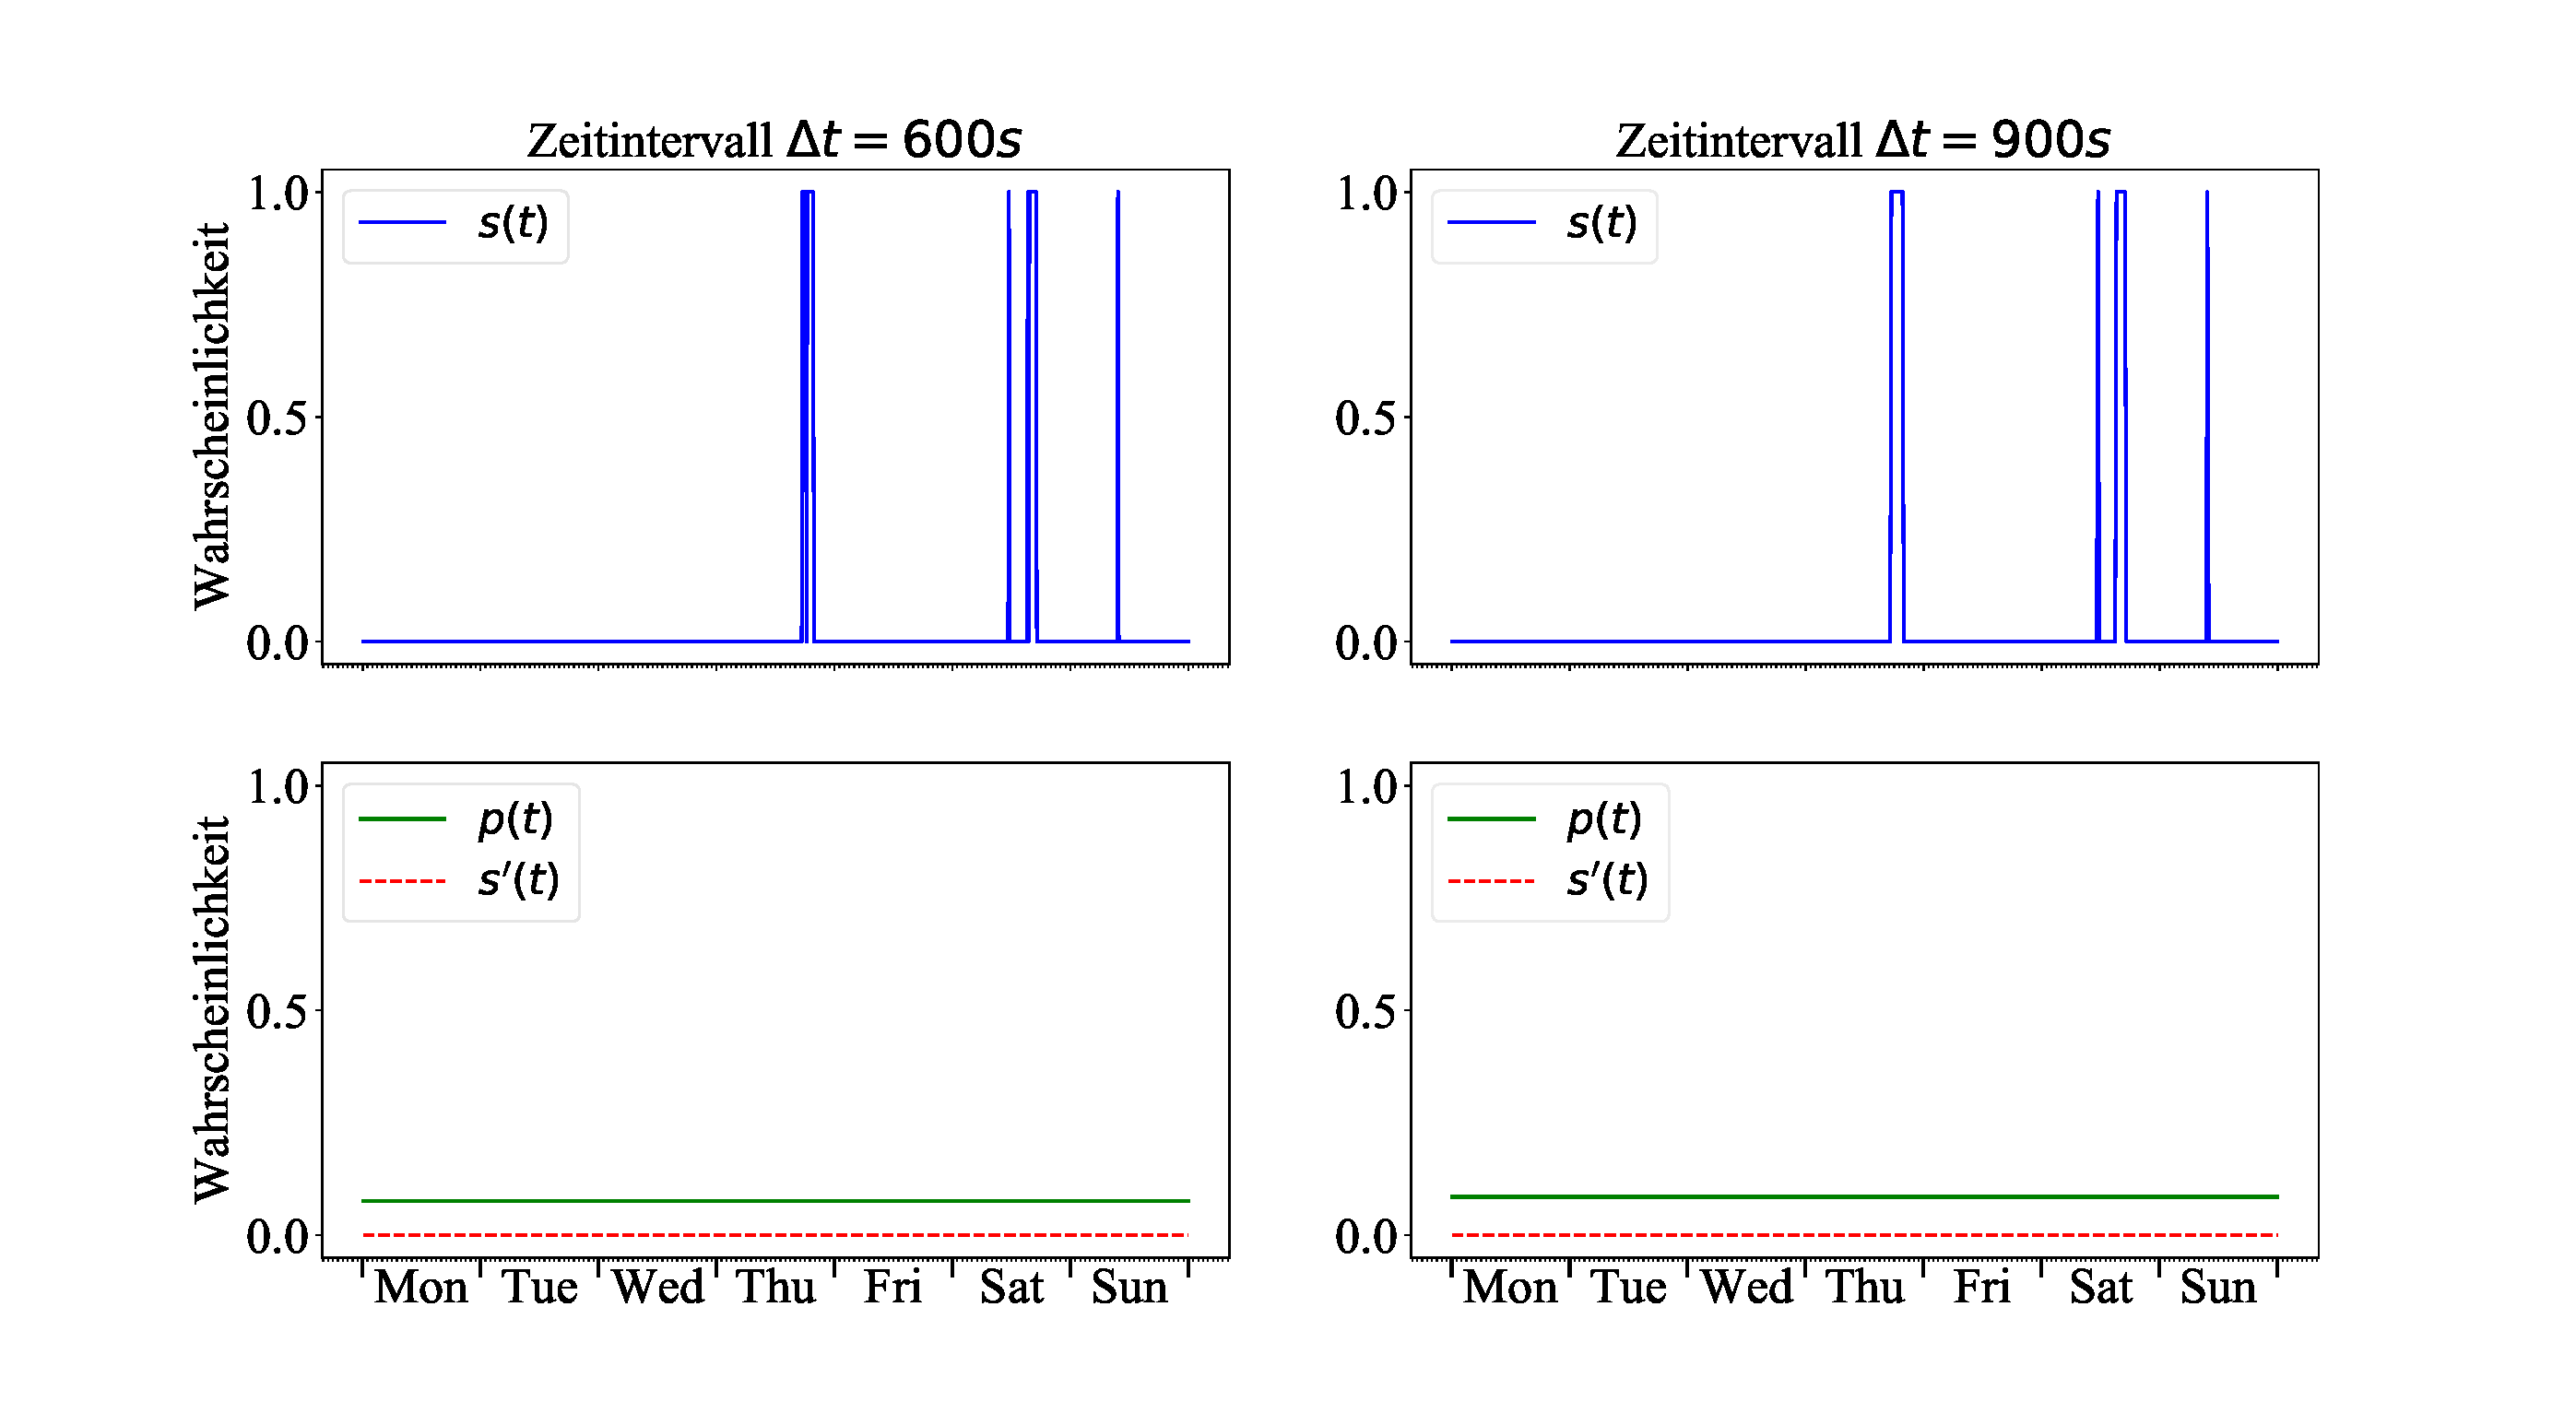
\includegraphics[width=\linewidth]{Abbildungen/evaluation/bin_size_influence_second_bedroom_binary.pdf}
		\caption[Zellzustand $s(t)$ sowie Wahrscheinlichkeitsfunktion $p(t)$ und prognostizierter Zellzustand $s'(t)$ des Gästeschlafzimmers des Apartments mit einer Intervalldauer von $\Delta t = \SI{600}{\second}$ und $\Delta t = \SI{900}{\second}$]{Zellzustand $s(t)$ sowie Wahrscheinlichkeitsfunktion $p(t)$ und prognostizierter Zellzustand $s'(t)$ des Gästeschlafzimmers des Apartments (Aruba-Datensatz) mit einer Intervalldauer von $\Delta t = \SI{600}{\second}$ (links) und $\Delta t = \SI{900}{\second}$ (rechts)}
		\label{fig.bin_size_influence_second_bedroom_binary}
	\end{center}
\end{figure}

Bei einer Intervalldauer von $\Delta t = \SI{600}{\second}$ ergibt sich die, nach Gleichung \ref{eq:Prädiktionsfehler}, optimale Modellordnung zu $l_\ind{opt}=0$, dargestellt durch die konstante, statische Wahrscheinlichkeitsfunktion $p_\ind{stat}(t)$. Zu dem selben Ergebnis kommt man bei einer Intervalldauer von $\Delta t = \SI{900}{\second}$. Auch hier beträgt die optimale Modellordnung $l_\ind{opt}=0$. Durch die Erhöhung der Personendetektionen im Vergleich zur Anzahl der Zeitstempel liegt die statische Wahrscheinlichkeit einer Personendetektion in der rechten, unteren Grafik von \bild{bin_size_influence_second_bedroom_binary} bei $p_\ind{stat}(t) = 7.9 \%$, während in der unteren linken Grafik $p_\ind{stat}(t) = 7.5 \%$ gilt. Die Personendetektionen beschränken sich auf seltene, kurzperiodige Bereiche, welche nicht durch die maximale Modellordnung von $l_\ind{max} = 20$ modelliert werden können. Eine weitere Erhöhung der Modellordnung würde dazu führen, dass der Rekonstruktionsfehler $\epsilon_\ind{r}$ zwar sinken würde, die Generalisierungsfähigkeit des Modells jedoch verloren geht und es in der Folge zu einem Anstieg des Prädiktionsfehlers $\epsilon_\ind{p}$ kommt. Der Prädiktionsfehler des statischen Modells bei einer Intervalldauer von $\Delta t = \SI{600}{\second}$ ergibt sich zu $\epsilon_\ind{p,stat} = 6.5 \%$, im Falle von $\Delta t = \SI{900}{\second}$ zu $\epsilon_\ind{p,stat} = 7.4 \% $. Erneut sei darauf hingewiesen, dass die Modelle mit den unterschiedlichen Intervalldauern nicht miteinander vergleichbar sind. Ein Vergleich kann lediglich gegenüber den zugehörigen, statischen Modellen, gezogen werden.\\
% Erklären: Warum ist das so? Grundbelegtheit nimmt durch Vergrößerung der Intervalle zu. Modell prognostiziert aber immer 0, sodass der Prädiktionsfehler steigt
Einen zusammenfassenden Überblick der Modellfehler gibt Tabelle \ref{tab.Prädiktionsfehler aruba_binary}.

\begin{table}[!h]
	\centering
	\caption{Prädiktionsfehler $\epsilon_\ind{p}$ bei unterschiedlichen Intervalldauern $\Delta t$ (Aruba)}\label{tab.Prädiktionsfehler aruba_binary}
	\vspace*{-3mm}
	\begin{tabular}{lcr}
		\toprule
		Intervalldauer $\Delta t$		& $\epsilon_\ind{p,opt}$ & $\epsilon_\ind{p,stat}$              \\
		\midrule
		\SI{300}{\second}	& 12.7 \%         & 20.4 \%  \\
		\rowcolor{Snow2}
		\SI{600}{\second} 	& 14.4 \%        & 23.42 \% \\
		\SI{900}{\second}   & 14.31 \%  & 22.99 \%	\\
		\bottomrule
	\end{tabular} 
\end{table}

Aufgeteilt nach unterschiedlichen Intervalldauern sind die Prädiktionsfehler $\epsilon_\ind{p}$ aller Zellen für die optimale Modellordnung $l_\ind{opt}$ sowie für den statischen Fall aufgeführt.
% Hier die Tabelle einfügen und noch ein paar Erläuterungen dazu äußern
Betrachtet werden jedoch nur Zellen bzw. Räume, welche während mindestens 5 \% der betrachteten Zeitintervalle $\Delta t_i$ belegt waren. Innerhalb des Aruba-Datensatzes erfüllen sieben der insgesamt zehn Zellen diese Anforderung. Die Begründung dieser Anforderung geht aus \bild{bin_size_influence_second_bedroom_binary} hervor. Die Modellierbarkeit kurzfristiger Zellenbelegtheiten ist limitiert. In diesen Fällen liegt das statische Modell mit einer prognostizierten, konstanten Zellenbelegtheit von $p(t) = \mathrm{const}. = 0$ bereits zu mindestens 95 \% richtig und würde so die Evaluierung der Methode verfälschen. Eine allgemeine Aussage über die optimale Modellordnung $l_\ind{opt}$ kann nicht getroffen werden. Wie in Abschnitt \ref{sec.Verarbeitung server binär} beschrieben wird, erstellt der Server für jede Zelle des Gitters ein separates Modell. Somit variiert auch die optimale Modellordnung je nach betrachteter Zelle. \\
% Anmerkung: ein sinnvoller Minimalwert kann glaube ich nicht angegeben werden, variiert ja von Modell zu Modell sehr stark
Eine weitere Evaluation erfolgt anhand des UOL-Datensatzes. Erneut werden die Modelle der insgesamt 3060 Zellen bei verschiedenen Intervalldauern $\Delta t$, in welche die Periodendauer $T$ eingeteilt wird, betrachtet. Wie in Abschnitt \ref{sec.Datensätze} erwähnt, werden zur Ermittlung der Modellparameter die Daten von zwei aufeinander folgenden Wochen benutzt. Die Ermittlung der optimalen Modellordnung $l_\ind{opt}$ mittels eines minimalen Prädiktionsfehlers $\epsilon_\ind{p,opt}$ erfolgt mit Daten einer weiteren, dritten Woche. \bild{bin_size_influence_cell_row_23_col_25_binary} zeigt die binären Modelle bei einer Intervalldauer von $\Delta t = \SI{600}{\second} $ (links) sowie für $\Delta t = \SI{900}{\second} $ (rechts). 
% Hier Abbildung bin_size_influence_cell_row_23_col_25_binary.pdf einfügen
\begin{figure}[!h]
	\centering
	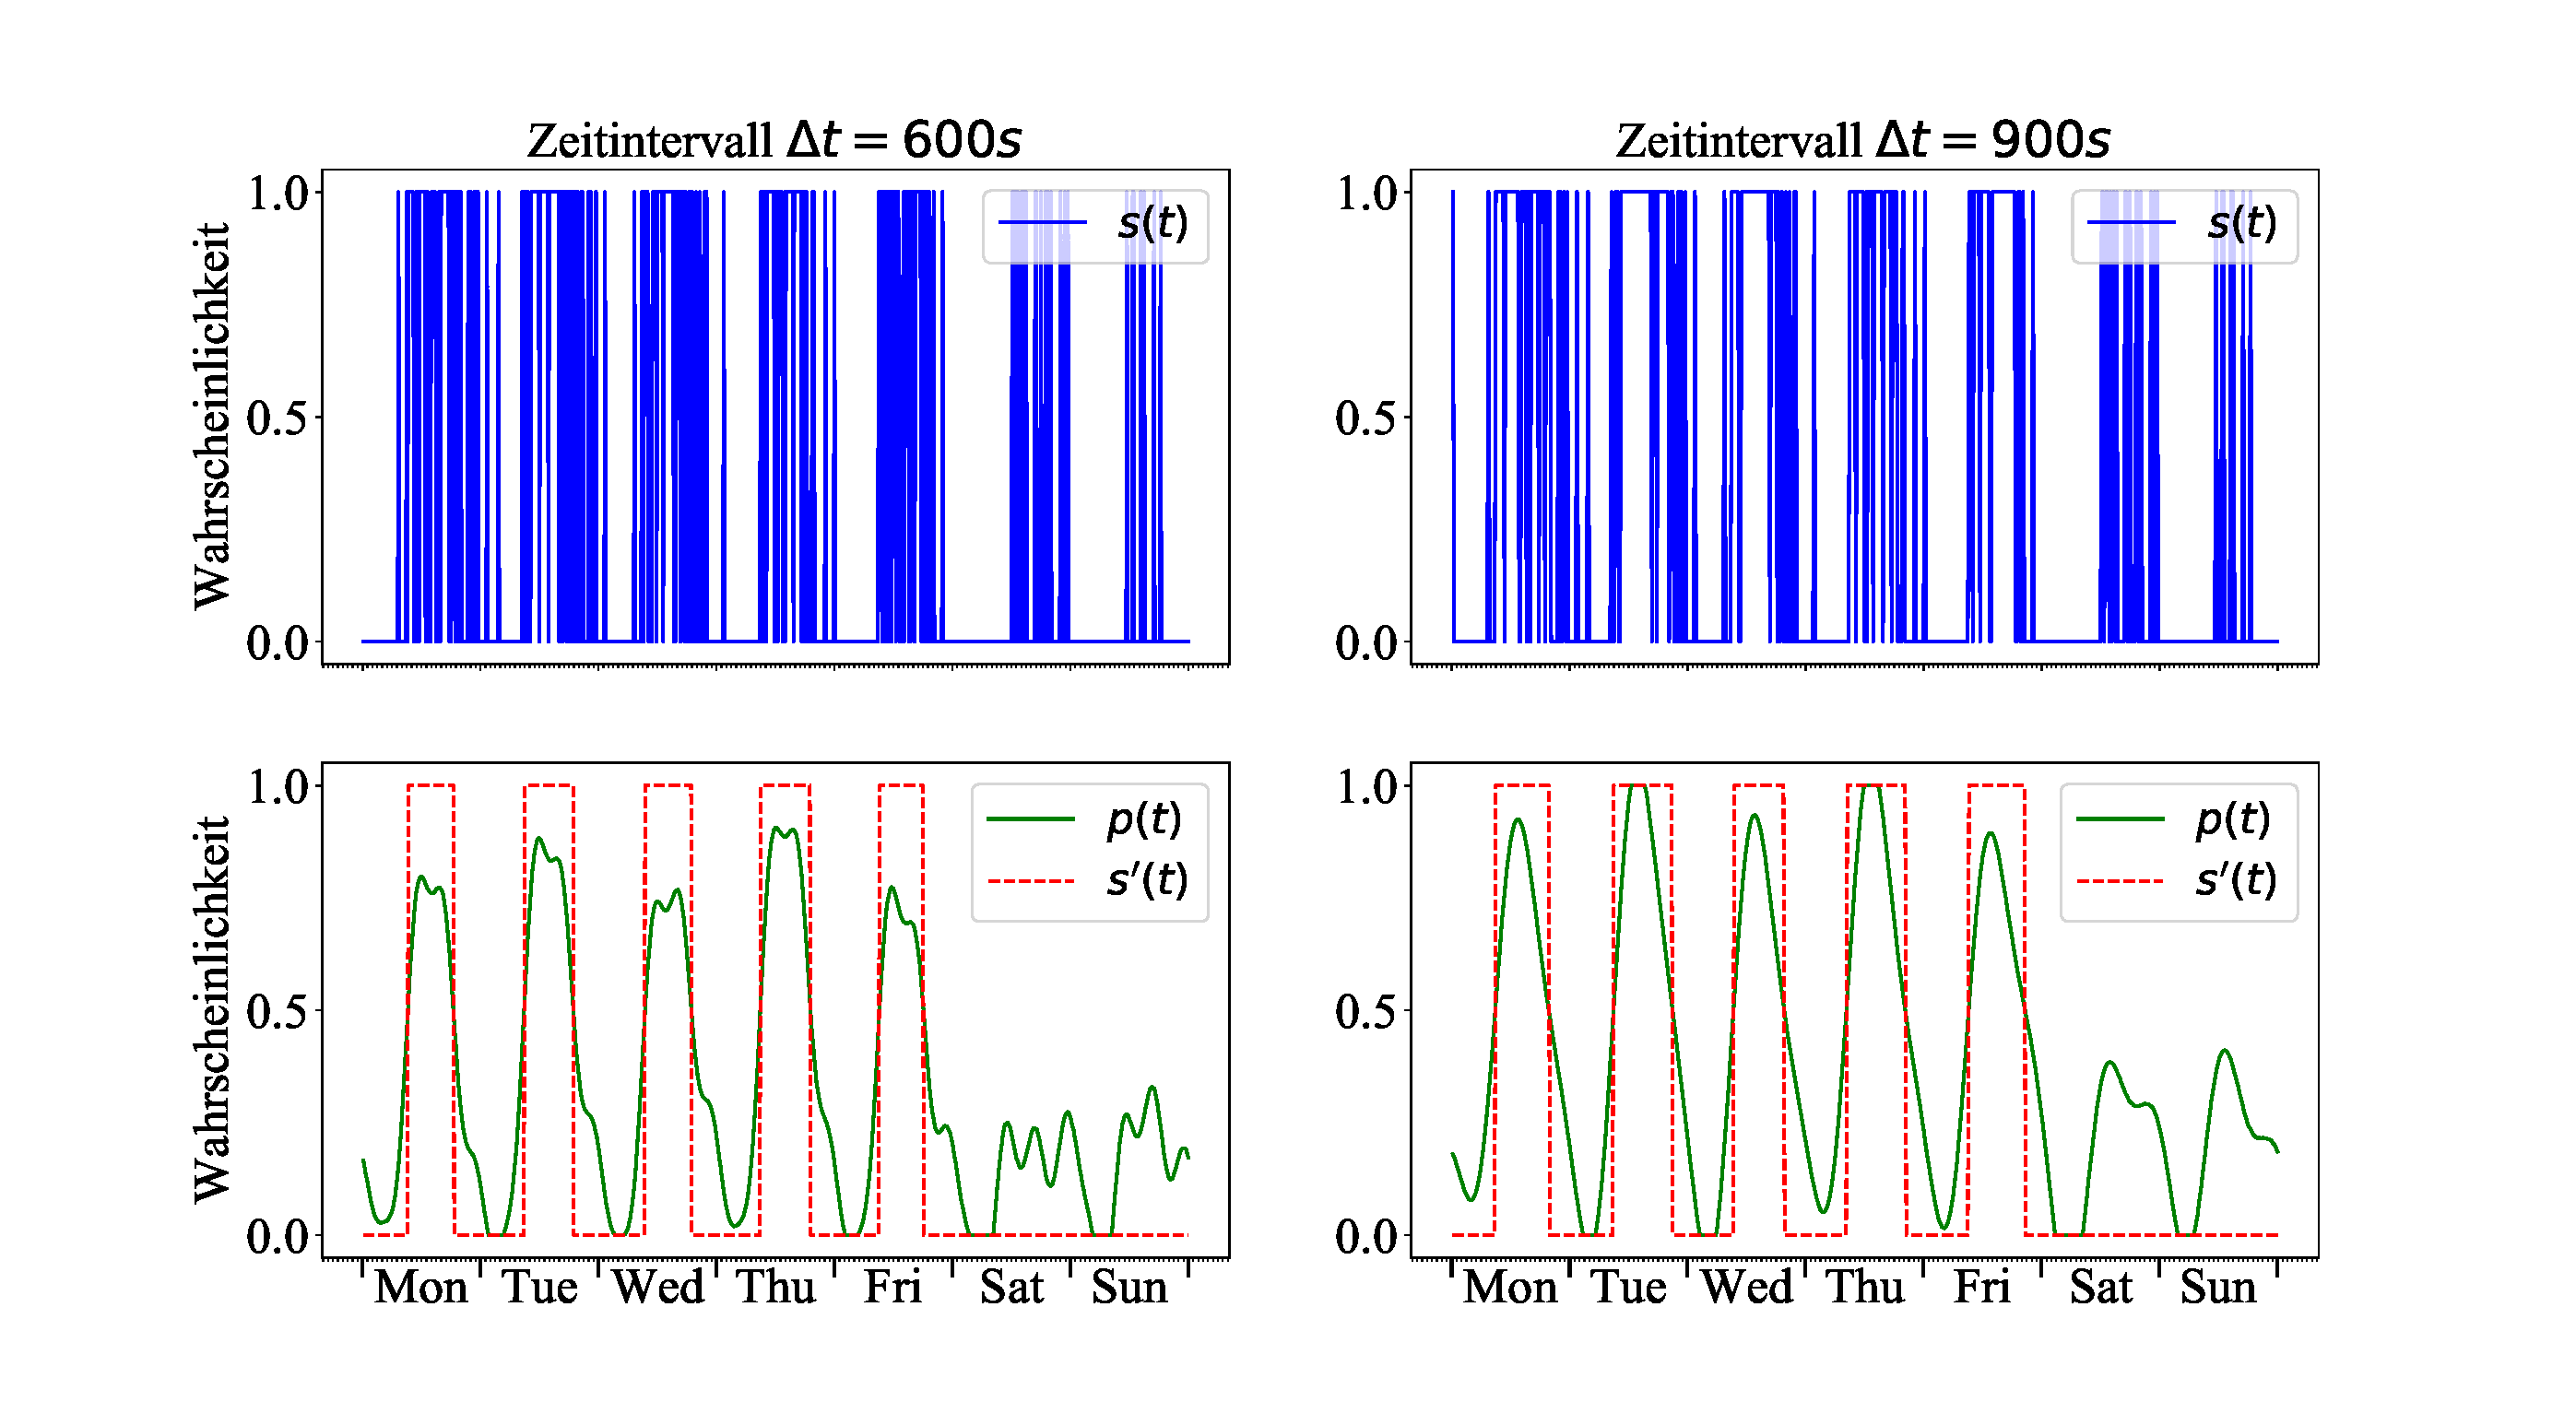
\includegraphics[width=1.0\linewidth]{Abbildungen/evaluation/bin_size_influence_cell_row_23_col_25_binary_numero_due}
	\caption{Zellzustand $s(t)$ sowie Wahrscheinlichkeitsfunktion $p(t)$ und prognostizierter Zellzustand $s'(t)$ einer Beispielzelle des UOL-Datensatzes mit einer Intervalldauer von $\Delta t = \SI{600}{\second} $ (links) und $\Delta t = \SI{900}{\second} $ (rechts)}
	\label{fig.bin_size_influence_cell_row_23_col_25_binary}
\end{figure}

Für die kürzere Intervalldauer $\Delta t = \SI{600}{\second}$ liegt die optimale Modellordnung bei $l_\ind{opt} = 10$ mit einem Prädiktionsfehler von $\epsilon_\ind{p,opt} = 15.1 \%$. Der Prädiktionsfehler des statischen Modells beträgt $\epsilon_\ind{p,stat} = 28.5 \%$. Es ist zu erkennen, dass das Modell den Wochentrend der Daten abbilden kann. An den beiden Wochenendtagen flachen die Amplituden der Wahrscheinlichkeitsfunktion des Zellzustandes $p(t)$ deutlich ab. Da sie den Schwellwert von $c = 0.5$ nicht überschreiten, liegt die Prädiktion des Zellzustandes während des Wochenendes bei $s'(t) = \mathrm{const}. = 0.0$. Bei einer Intervalldauer von $\Delta t = \SI{900}{\second} $ berechnet sich die optimale Modellordnung zu $l_\ind{opt} = 7$. Wie in \bild{bin_size_influence_master_bedroom_binary} resultiert eine Erhöhung der Intervalldauer $\Delta t$ in einer Vergrößerung der Breite der rot gestrichelten Balken der Prädiktion des Zellzustandes $s'(t)$. Erklären lässt sich dieses Verhalten damit, dass eine Verlängerung der Intervalldauer $\Delta t$ nach Gleichung \ref{eq:Number timestamps} zu einer Erhöhung des durchschnittlichen Zellzustandes $\bar{s}(t)$ führt. Auch das Modell der größeren Intervalldauer $\Delta t = \SI{900}{\second}$ kann den Wochentrend mit einem Abflachen der Personen-Auftrittswahrscheinlichkeiten während des Wochenendes abbilden. Liegt der Prädiktionsfehler der optimalen Modellordnung bei $\epsilon_\ind{p,opt} = 13.8 \%$, so beträgt er bei dem statischen Zustandsmodell $\epsilon_\ind{p,stat} = 35.3 \%$. \\
Einen zusammenfassenden Überblick der Modellfehler gibt Tabelle \ref{tab.Prädiktionsfehler uol_binary}.

\begin{table}[!h]
	\centering
	\caption{Prädiktionsfehler $\epsilon_\ind{p}$ bei unterschiedlichen Intervalldauern $\Delta t$ (UOL)}\label{tab.Prädiktionsfehler uol_binary}
	\vspace*{-3mm}
	\begin{tabular}{lcr}
		\toprule
		Intervalldauer $\Delta t$		& $\epsilon_\ind{p,opt}$	 & $\epsilon_\ind{p,stat}$          \\
		\midrule
		\SI{300}{\second}	& 8.93 \%         & 9.03 \%  \\
		\rowcolor{Snow2}
		\SI{600}{\second} 	& 10.49 \%        & 11.62 \% \\
		\SI{900}{\second}			& 10.75 \%      & 12.92 \% \\
		\bottomrule
	\end{tabular} 
\end{table}

% Auf Ergebnisse der Tabelle eingehen. Evtl letzte Spalte entfernen
% Betrachtet wurden nur Zellen, welche in mindestens fünf Prozent der Intervalle belegt % waren.

Aufgeteilt nach Intervalldauern sind hier die Prädiktionsfehler $\epsilon_\ind{p}$ aller Zellen für die optimale Modellordnung $l_\ind{opt}$ sowie für das statische Zustandsmodell aufgelistet. Es werden erneut nur die Zellen betrachtet, welche während mindestens 5 \% der betrachteten Zeitintervalle $\Delta t_i$ belegt waren. Diese Voraussetzung erfüllen nur 205 der insgesamt 3060 Zellen, in welche die Umgebung $\mathcal{U}$ eingeteilt wird.

Eine Darstellung des über die Umgebung $\mathcal{U}$ gelegten Gitters mit seinen einzelnen Zellen bietet \bild{original_binary_data}. Für ein beispielhaftes Zeitintervall $\Delta t_i$ mit einer Dauer von $\Delta t = \SI{600}{\second}$ ist hier für jede Zelle der zugehörige Zellstatus s(t) farblich dargestellt.



Zellen, welche innerhalb des Zeitintervalls belegt waren, sind in der Grafik rot markiert. Die restlichen, in blau eingefärbten Zellen, weisen während des entsprechenden Zeitintervalls keine Personendetektionen vor. Ein grafischer Vergleich zwischen den, mittels der optimalen Modellordnungen $l_\ind{opt}$ berechneten FreMEn-Modellen und den statischen Modellen der einzelnen Zellen kann mit Hilfe von \bild{binary_fremen_vs_static} gezogen werden.
\newpage
% caption ändern !
\begin{figure}[!ht]
	\centering
	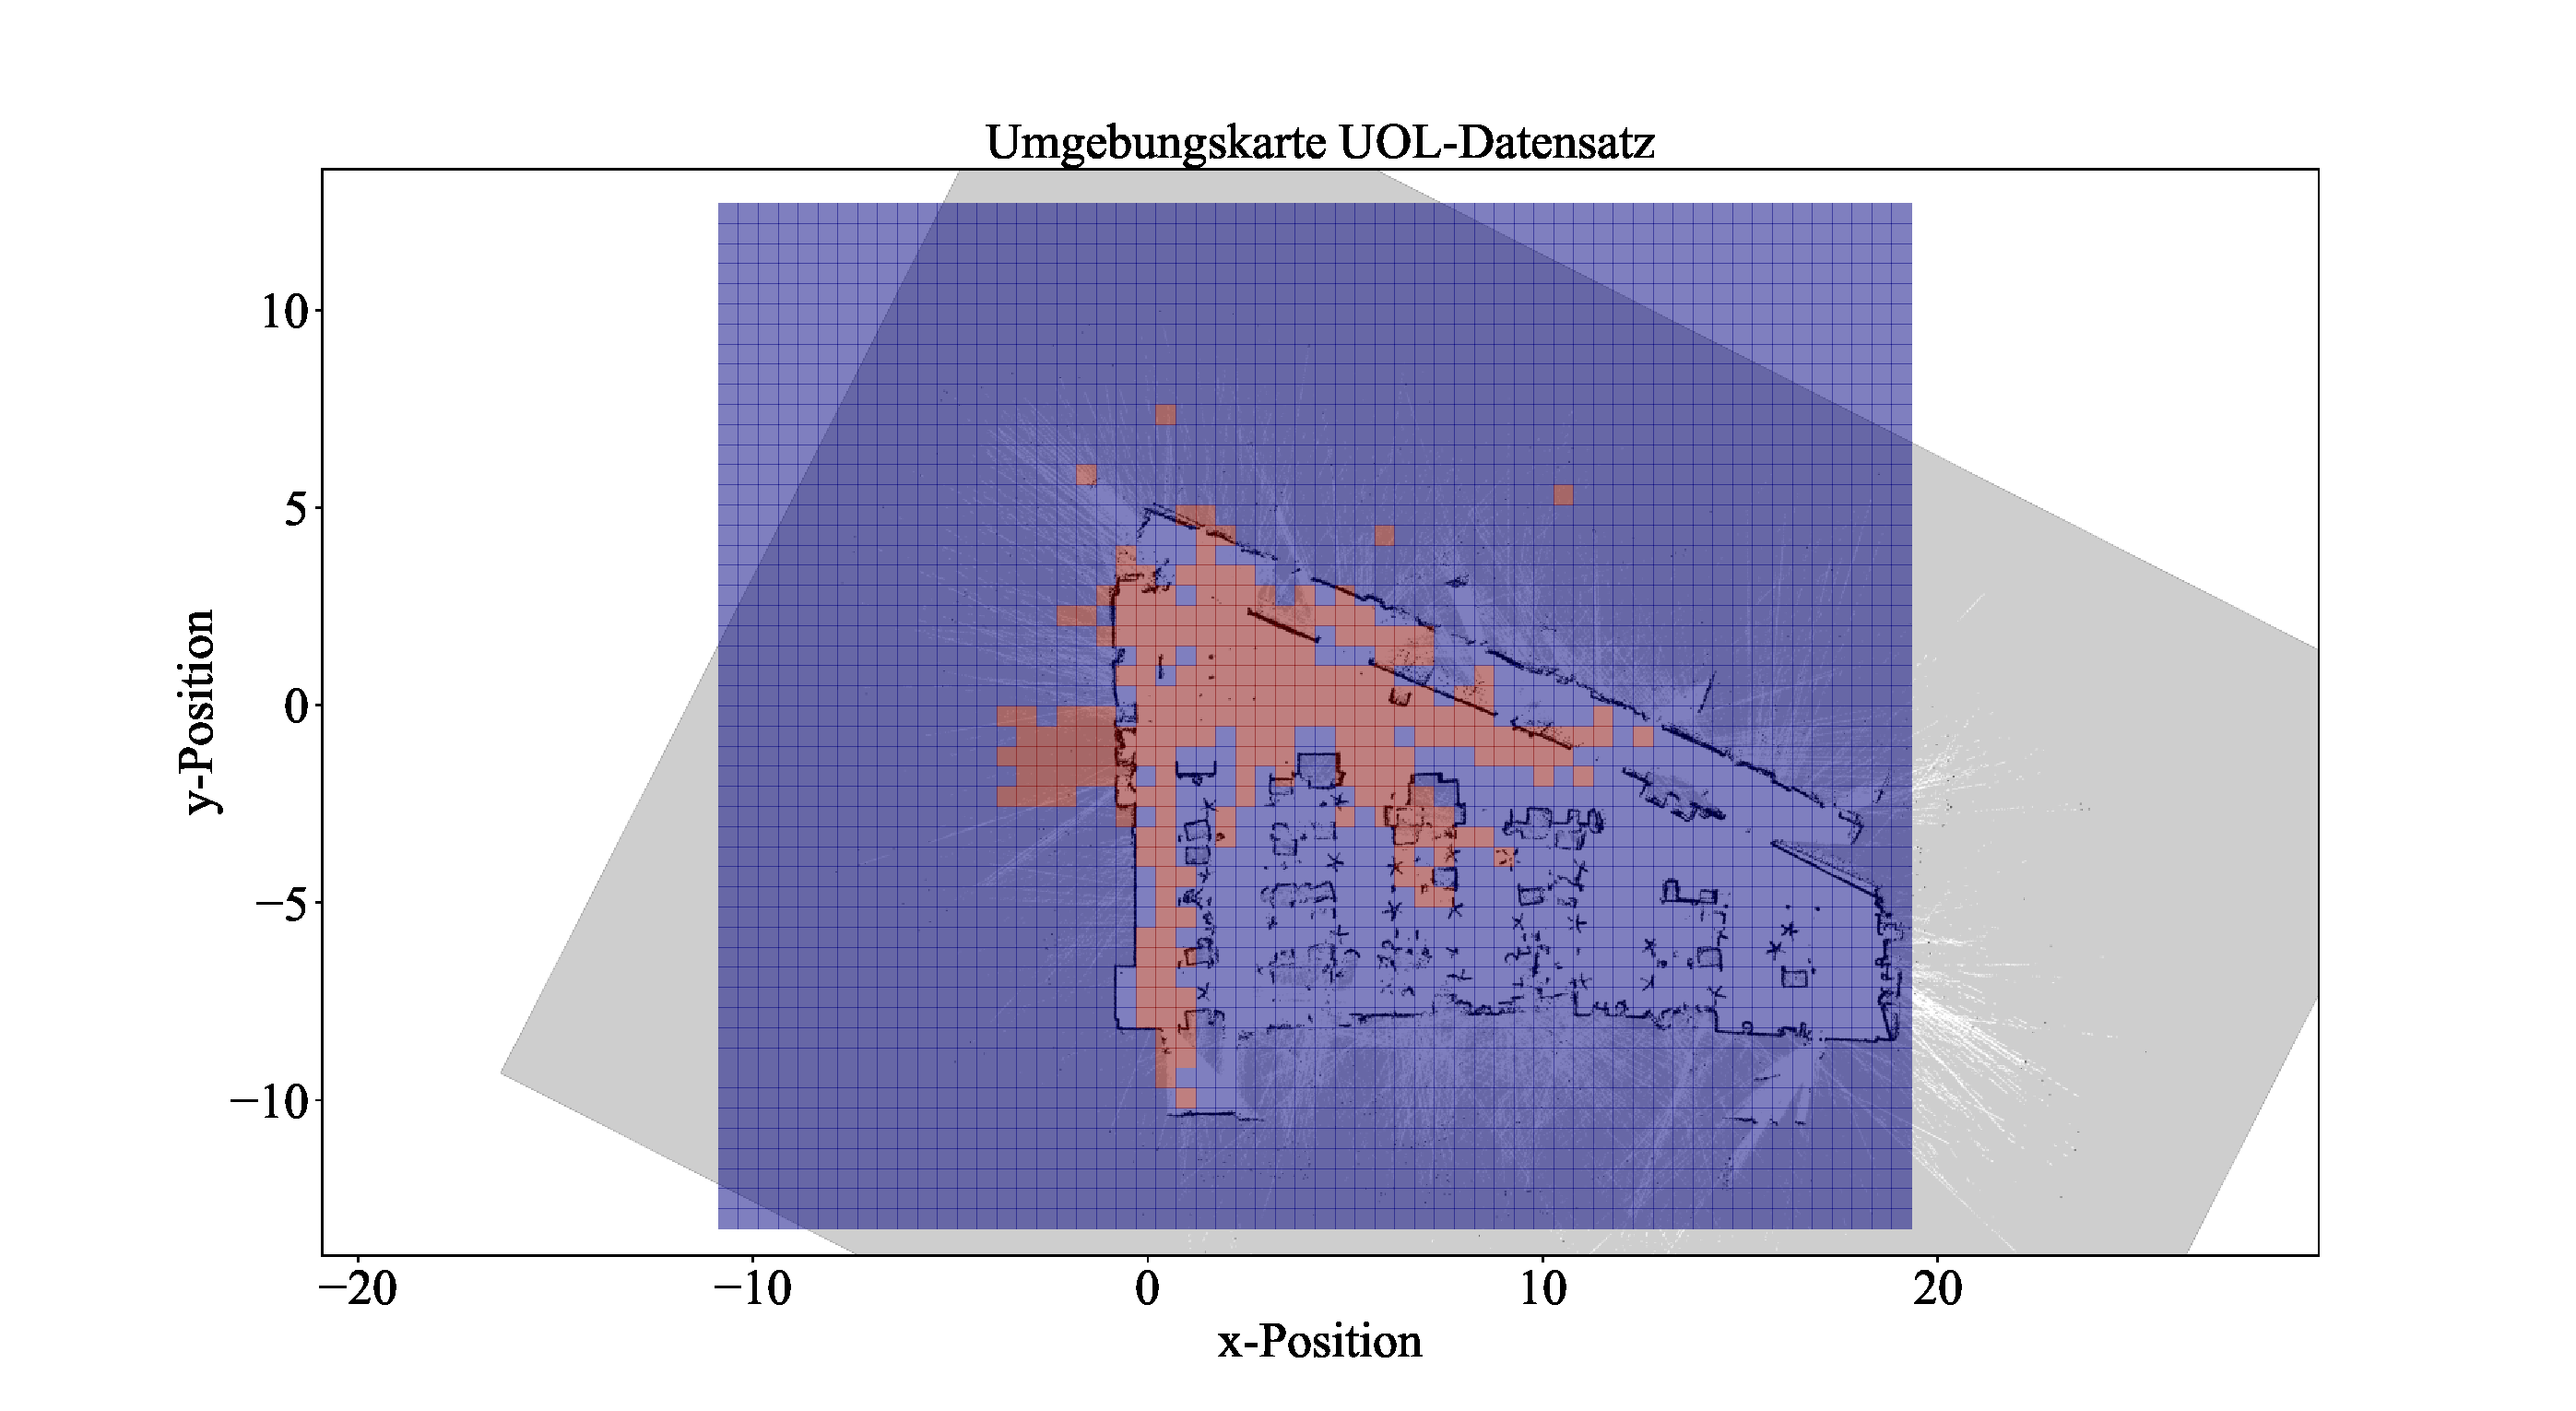
\includegraphics[width=1.0\linewidth]{Abbildungen/evaluation/original_binary_data}
	\caption{Tatsächliche Zellzustände s(t) des Belegungsgitters innerhalb eines beispielhaften Zeitintervalls $\Delta t_i$}
	\label{fig.original_binary_data}
\end{figure}
Zu erkennen ist, dass die FreMEn-Modelle (Bild \ref{fig.binary_best_prediction}) nur einen Teil der Gesamtheit der belegten Zellen als solche prognostizieren. Die als \textit{belegt} prognostizierten Zellen befinden sich allesamt innerhalb des Bürogebäudes. Die außerhalb des Gebäudes befindlichen, belegten Zellen (vlg. \bild{original_binary_data}) überschreiten im FreMEn-Modell nicht den Schwellwert von $c=0.5$ und werden somit als \textit{frei} prognostiziert. In Bild \ref{fig.binary_static} ist das statische Modell der einzelnen Zellen des Gitters dargestellt. Man erkennt, dass keine der Zellen innerhalb des betrachteten Zeitintervalls als \textit{belegt} prognostiziert worden ist. Die Begründung liegt darin, dass keine der einzelnen Zellen einen über den Gesamtzeitraum durchschnittlichen Zellzustand von $\bar{s(t)} = 0.5$ besitzt. Somit kann für keine Zelle der Schwellwert von $c=0.5$ überschritten werden. 

\begin{figure}[!h]
	\centering
	\subfigure[Prognostizierte Zellzustände s'(t) mit FreMen-Modellen der Ordnungen $l_\ind{opt}$\label{fig.binary_best_prediction}]{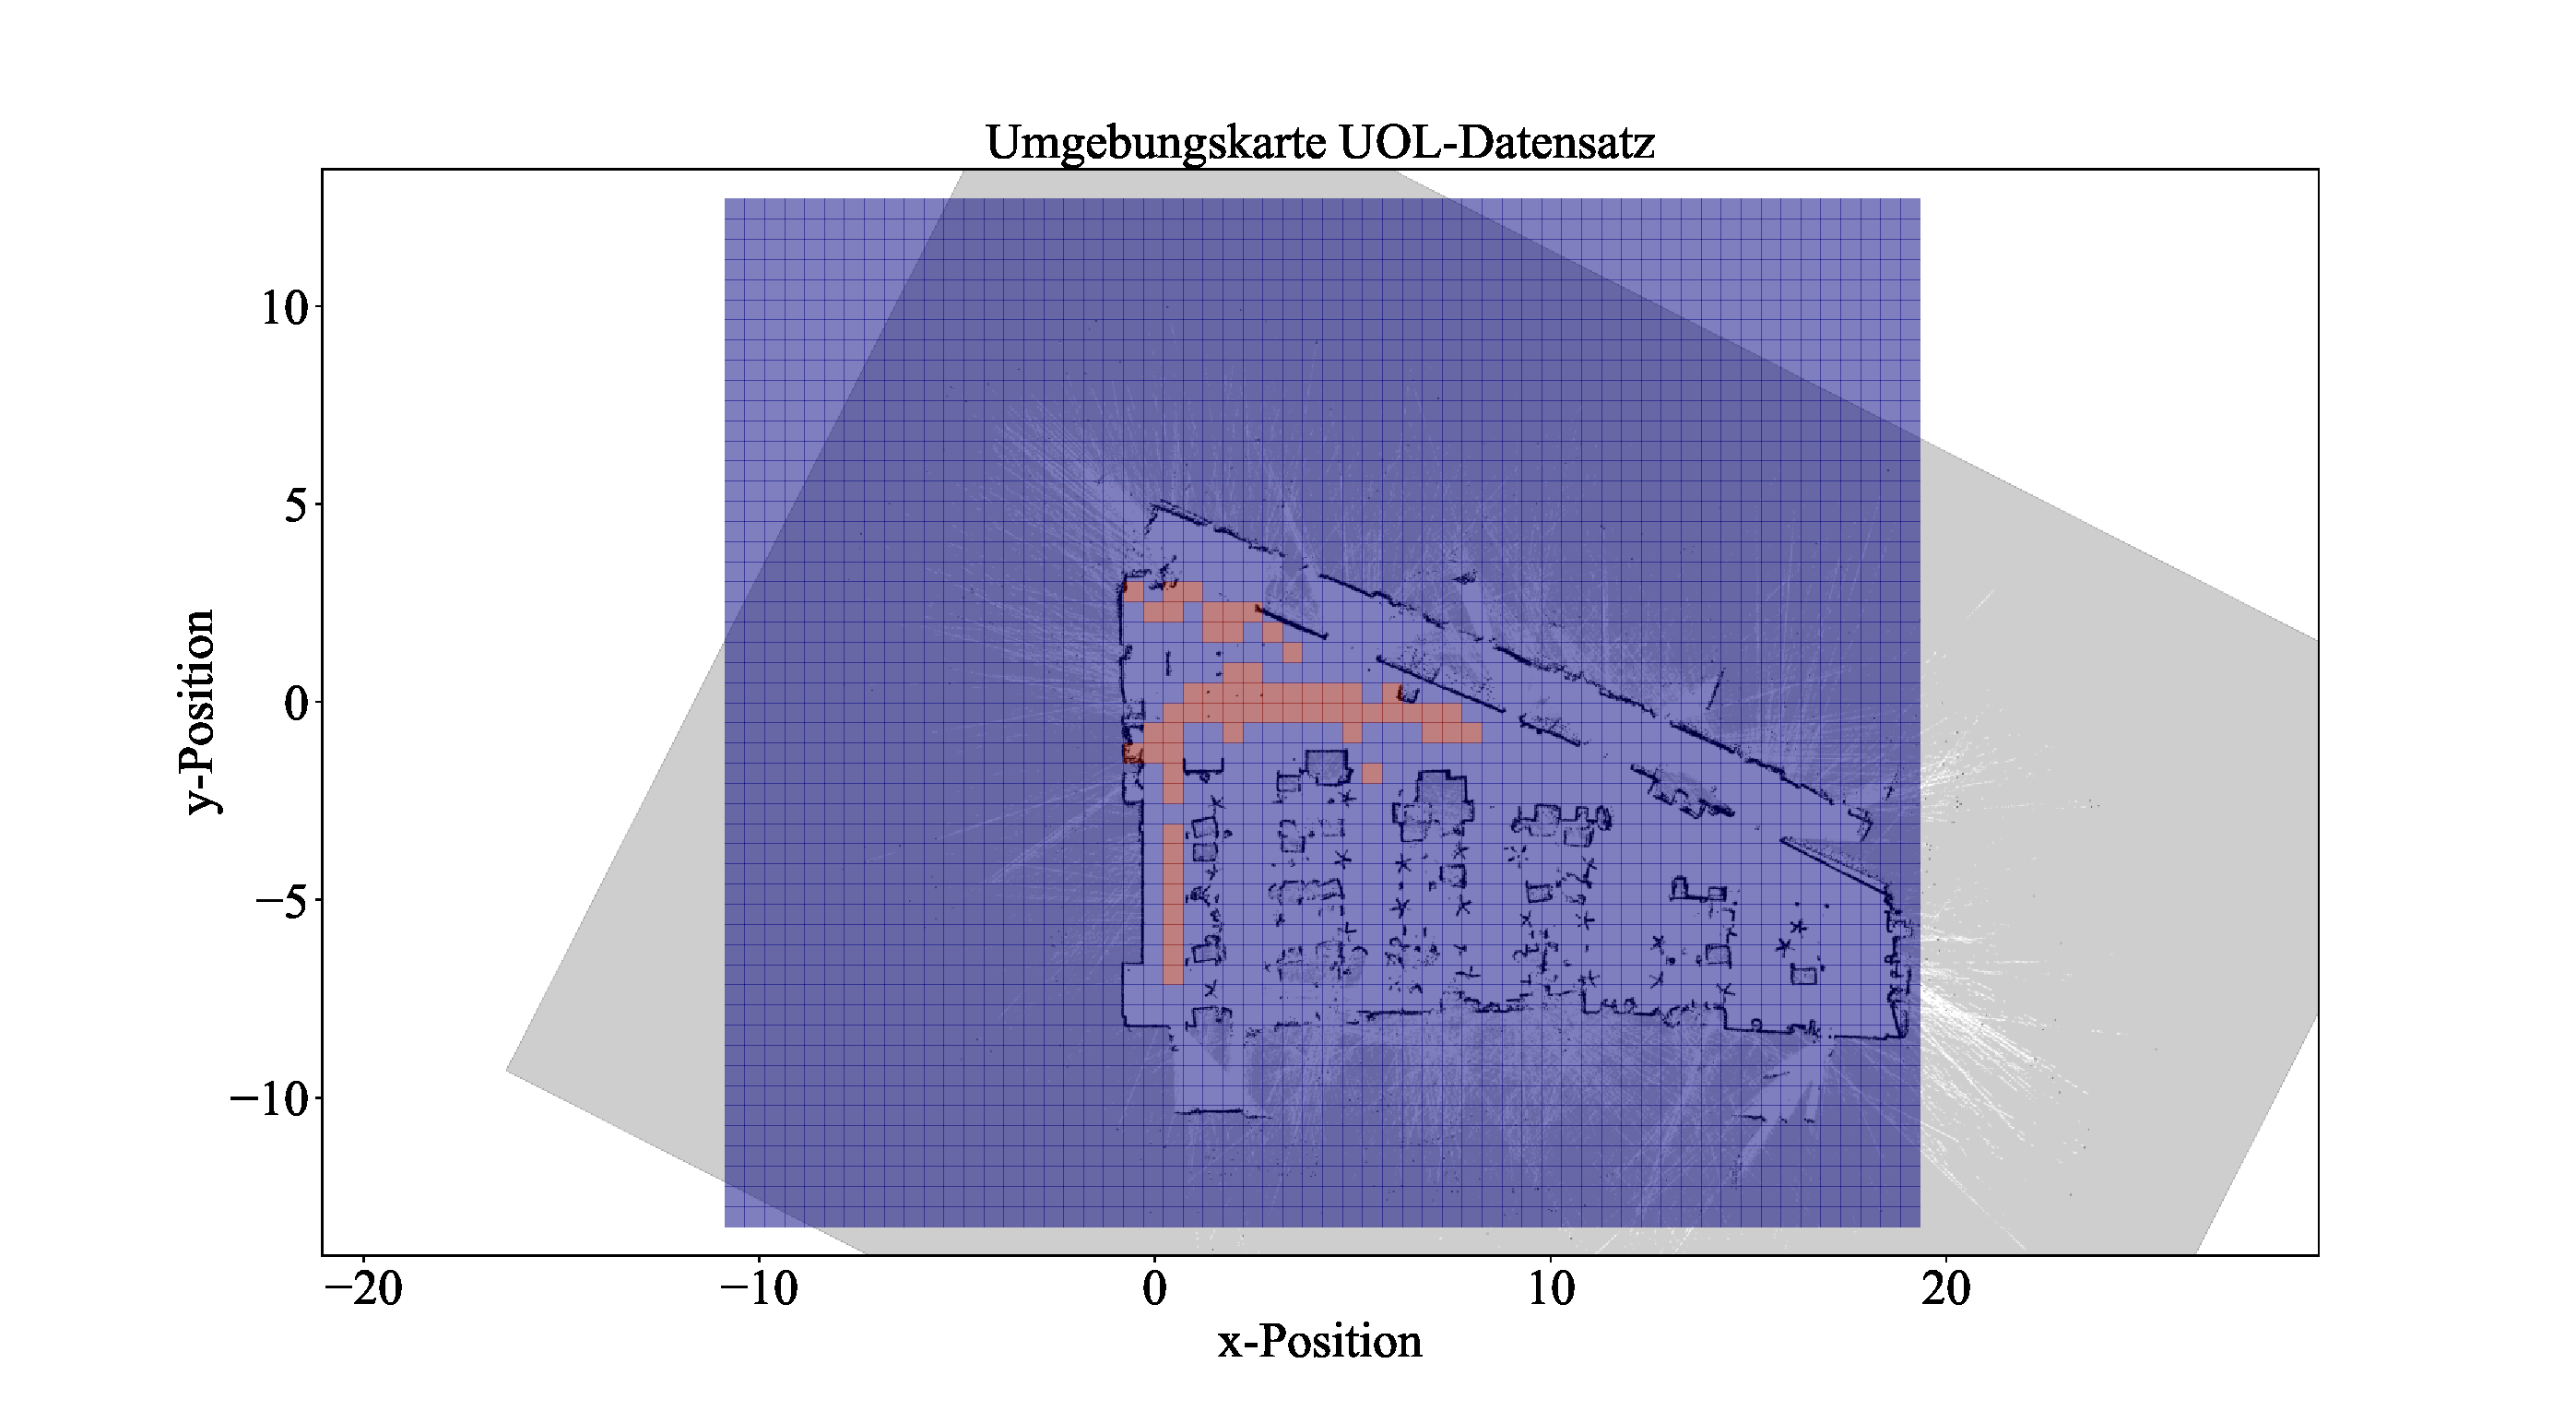
\includegraphics[width=1.0\linewidth]{Abbildungen/evaluation/binary_data_best_prediction}}

	\subfigure[Prognostizierte Zellzustände s'(t) mit statischen Modellen\label{fig.binary_static}]{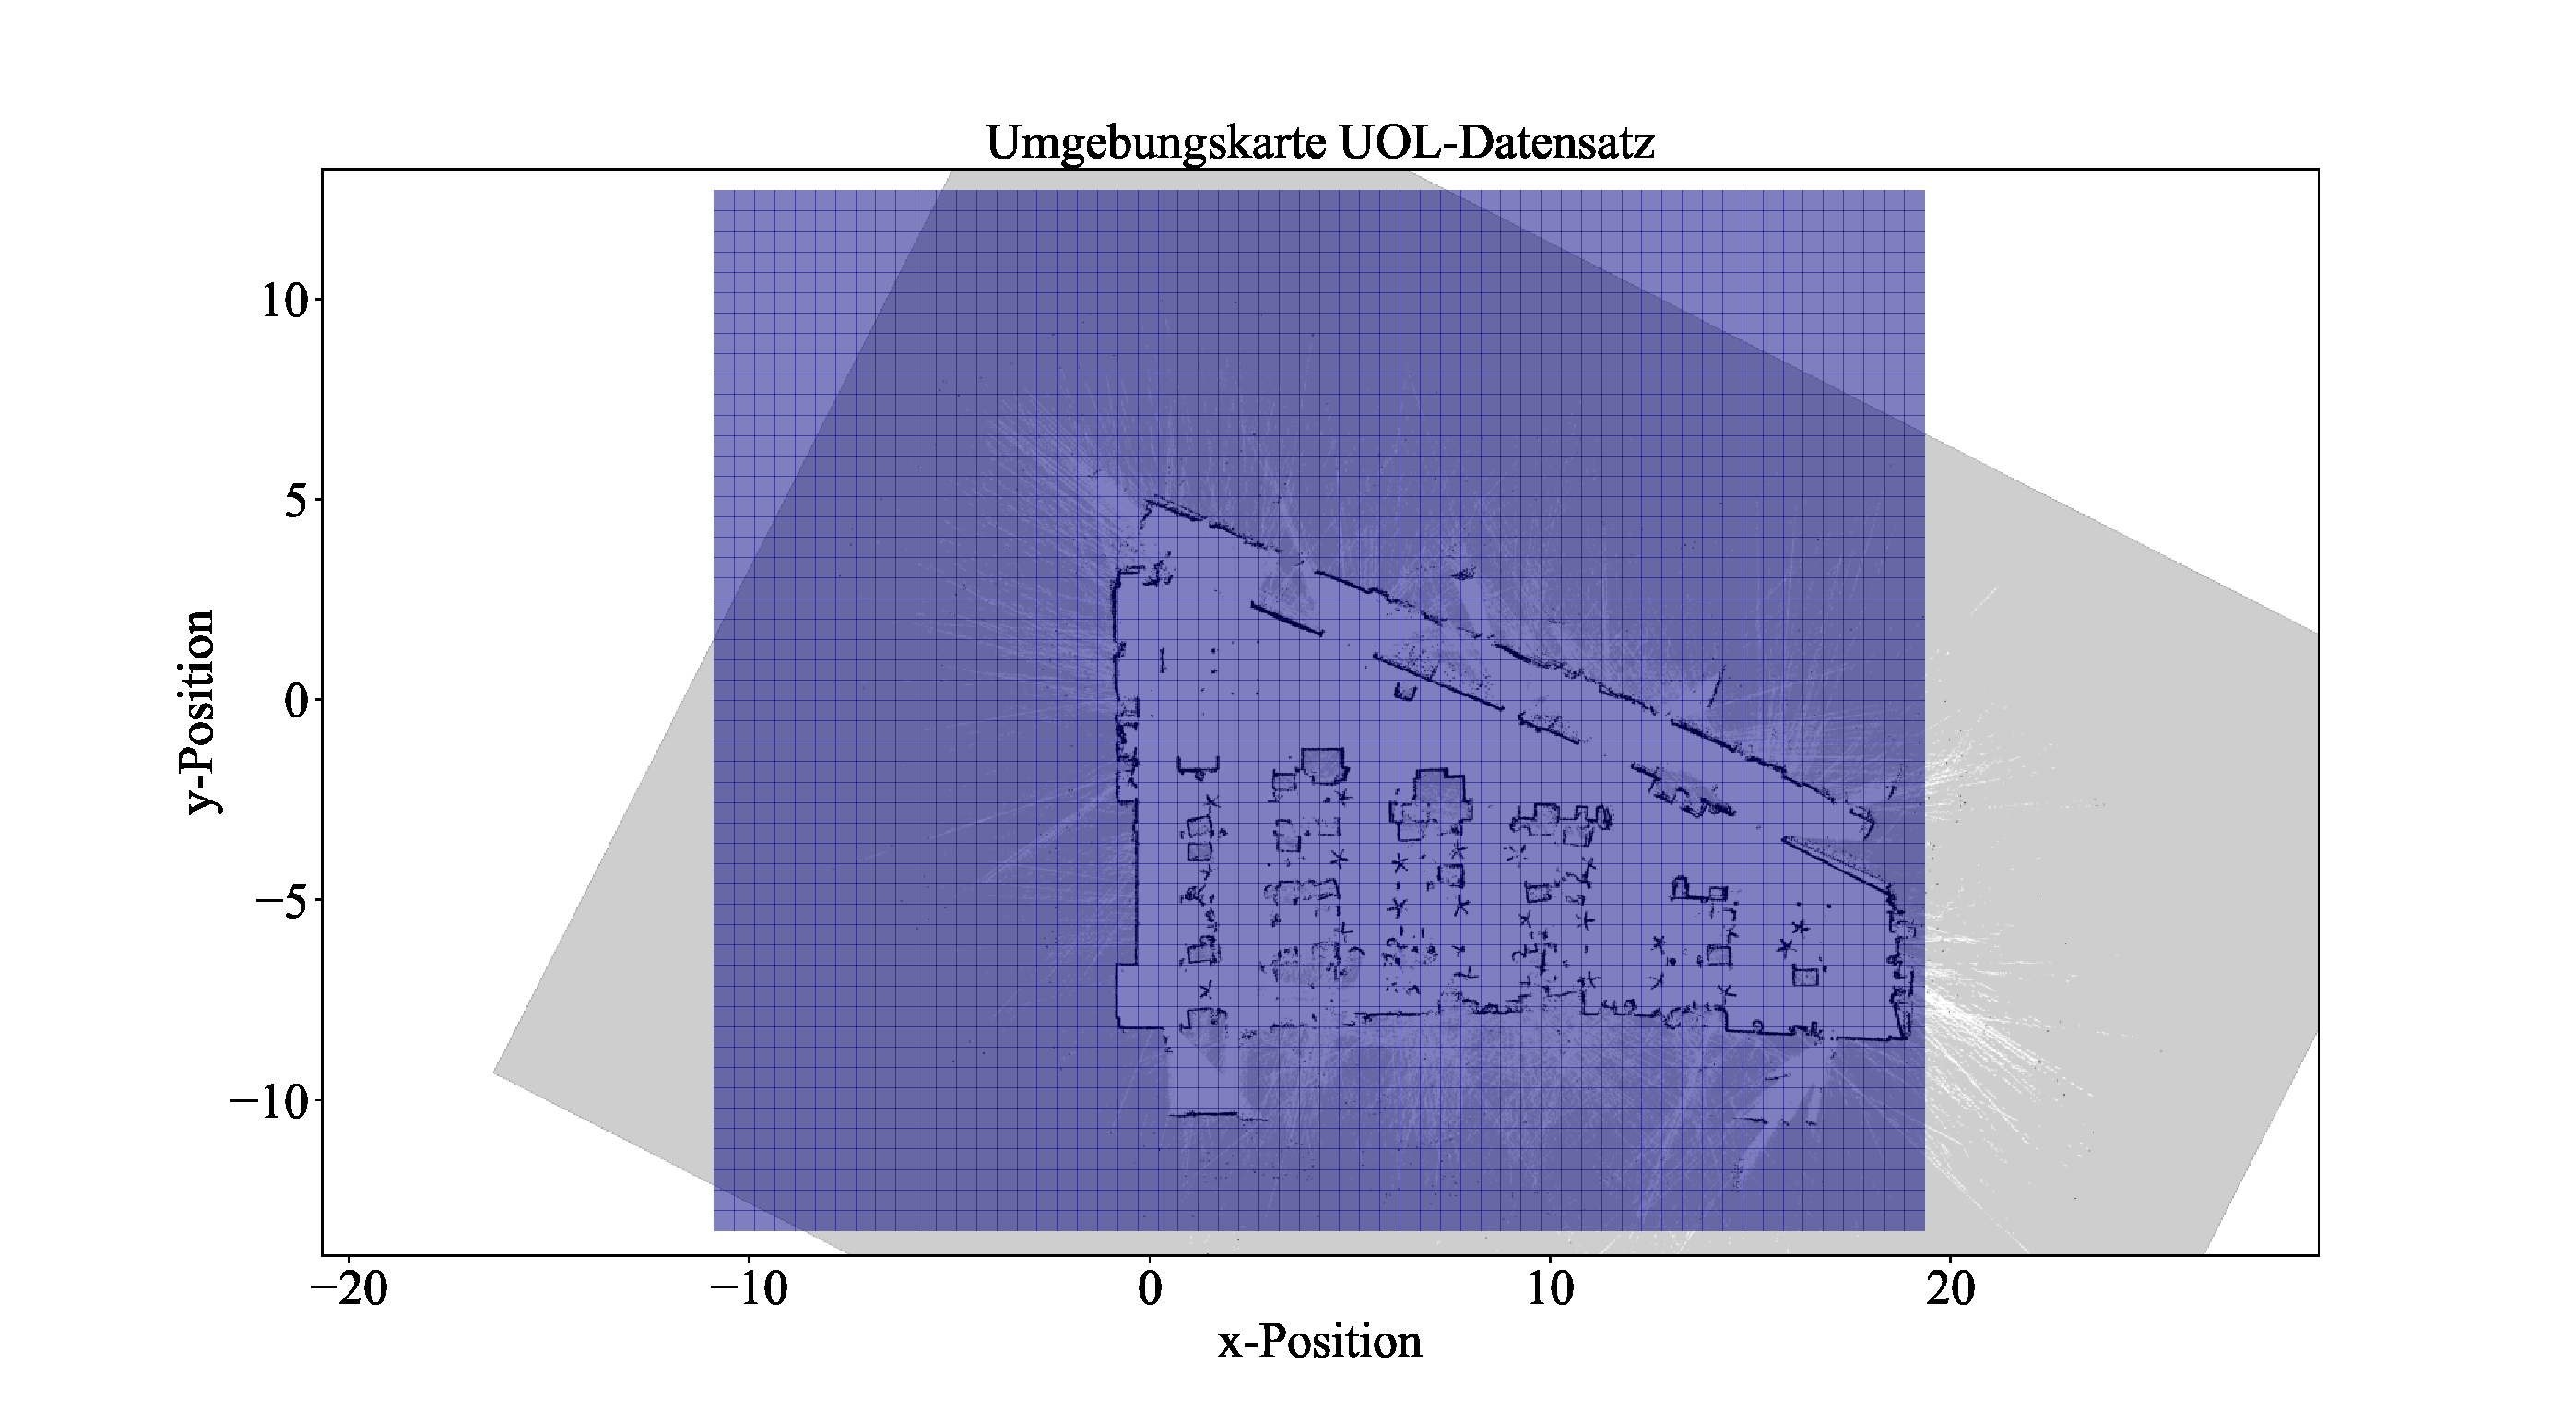
\includegraphics[width=1.0\linewidth]{Abbildungen/evaluation/binary_data_static}}
	\caption{Vergleich von FreMEn-Modellen mit statischen Modellen für den binären Fall}
	\label{fig.binary_fremen_vs_static}
\end{figure}



\newpage
\section{Quantitatives Modell}
\label{sec.Quantitatives Modell}

In diesem Abschnitt erfolgt eine Evaluation der quantitativen Modelle. Der betrachtete Wert ist die Personenrate $\lambda(t)$, also die Anzahl von Personen innerhalb eines Zeitintervalls. Veranschaulicht wird dies in \bild{bin_size_influence_master_bedroom_float_600}.

\begin{figure}[!h]
	\begin{center}
		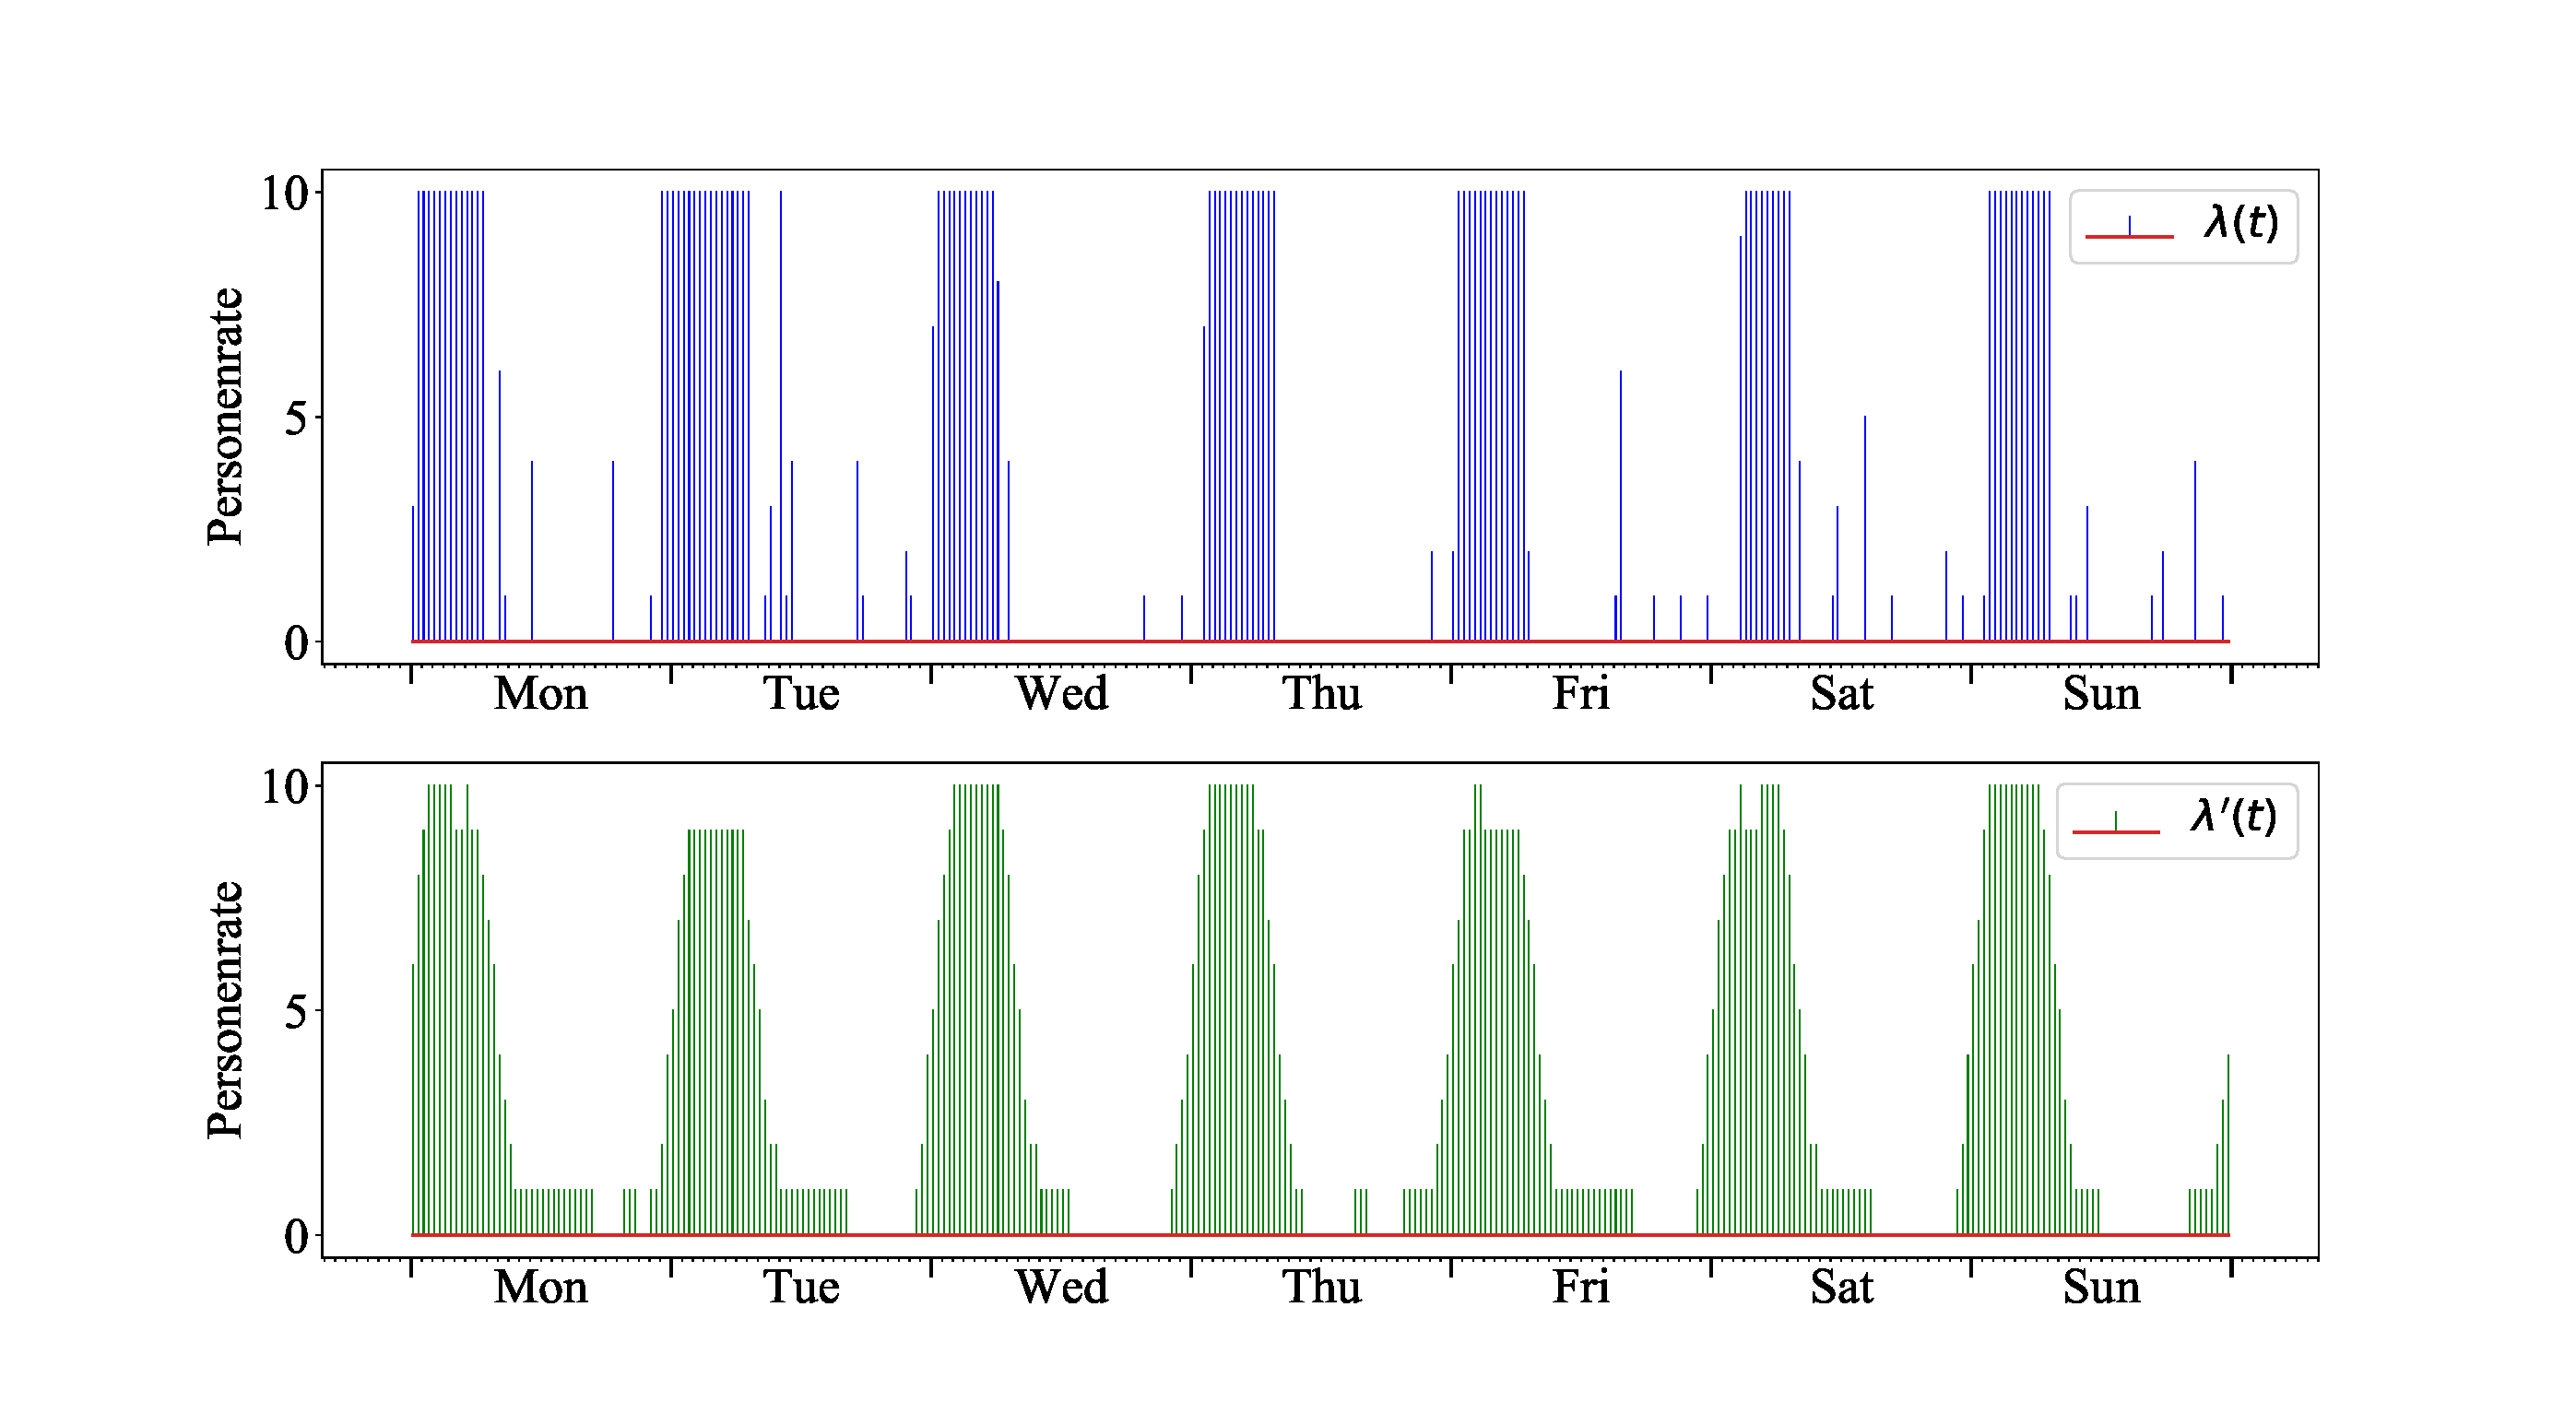
\includegraphics[width=\linewidth]{Abbildungen/evaluation/bin_size_influence_master_bedroom_float_600.pdf}
		\caption[Personenrate $\lambda (t)$  des Schlafzimmers (Aruba Datensatz) bei einer Intervalldauer von  $\Delta t = \SI{600}{\second}$ und Approximation $\lambda '(t)$]{Personenrate $\lambda (t)$  des Schlafzimmers (Aruba-Datensatz) bei einer Intervalldauer von  $\Delta t = \SI{600}{\second}$ (oben) und Approximation $\lambda '(t)$ (unten)}
		\label{fig.bin_size_influence_master_bedroom_float_600}
	\end{center}
\end{figure}

Dargestellt sind die Personenraten $\lambda (t)$ des Schlafzimmers des Aruba-Datensatzes  bei einer Intervalldauer von $\Delta t = \SI{600}{\second}$ (oben). Im Aruba-Datensatz wurde der Aufenthaltsort einer Person innerhalb der Räume der Wohnung minütlich dokumentiert. Die in \bild{bin_size_influence_master_bedroom_float_600} gewählte Intervalldauer resultiert also in einer maximalen Personenrate von $\lambda_\ind{max} = 10$. Im Bezug auf den Begriff \textit{Personenrate} sei angemerkt, dass sich diese im vorliegenden Zusammenhang lediglich auf dieselbe, innerhalb der Wohnung befindliche, Person bezieht.  Die optimale Modellordnung zur Berechnung von $\lambda '(t)$, also der Approximation der tatsächlichen Personenrate $\lambda(t)$, liegt bei $l_\ind{opt}=5$. Die Approximation ist in der unteren Grafik von \bild{bin_size_influence_master_bedroom_float_600} aufgezeichnet. Der Prädiktionsfehler  ergibt sich zu $\epsilon_\ind{p,opt} = 2.61$. Der Fehler wurde nach Gleichung \ref{eq:Prädiktionsfehler quantitativ} berechnet, die von dem Modell prognostizierte Personenrate $\lambda ' (t) $ hat also eine durchschnittliche Abweichung von 2.61 Personen pro Intervall von den tatsächlichen Daten. Die statische Personenrate beträgt $\lambda_\ind{stat} ' (t) = 4$. Der Prädiktionsfehler des statischen Modells liegt bei $\epsilon_\ind{p,stat} = 4.46$.
% In der oberen Grafik muss noch die statische Personenrate lambda_stat als gestrichelte gelbe Linie eingezeichnet werden.

\bild{bin_size_influence_master_bedroom_float_900} stellt $\lambda(t)$ bei einer Intervalldauer von $\Delta t = \SI{900}{\second}$ dar. Im Vergleich zu \bild{bin_size_influence_master_bedroom_float_600} liegen die Peaks von $\lambda (t)$ hier höher, was durch die größere Intervalldauer begründet ist. Die untere Grafik von \ref{fig.bin_size_influence_master_bedroom_float_900} stellt erneut die im Sinne von Gleichung \ref{eq:Prädiktionsfehler quantitativ} optimale Approximation $\lambda ' (t)$ von $\lambda (t)$ dar. Die optimale Modellordnung liegt erneut bei $l_\ind{opt} = 5$. Der Prädiktionsfehler liegt hier bei $\epsilon_\ind{p,opt} =  3.81$. Die Personenrate des statischen Modells lautet $\lambda_\ind{stat} ' = 5$. Der Prädiktionsfehler des statischen Modells beträgt $\epsilon_\ind{p,stat} = 6.62$. \\
Im Vergleich zum statischen Modell kann also mit einer Modellordnung von $l_\ind{opt} = 5$ eine Verbesserung um 43.45 \% erreicht werden.

\begin{figure}[!h]
	\begin{center}
		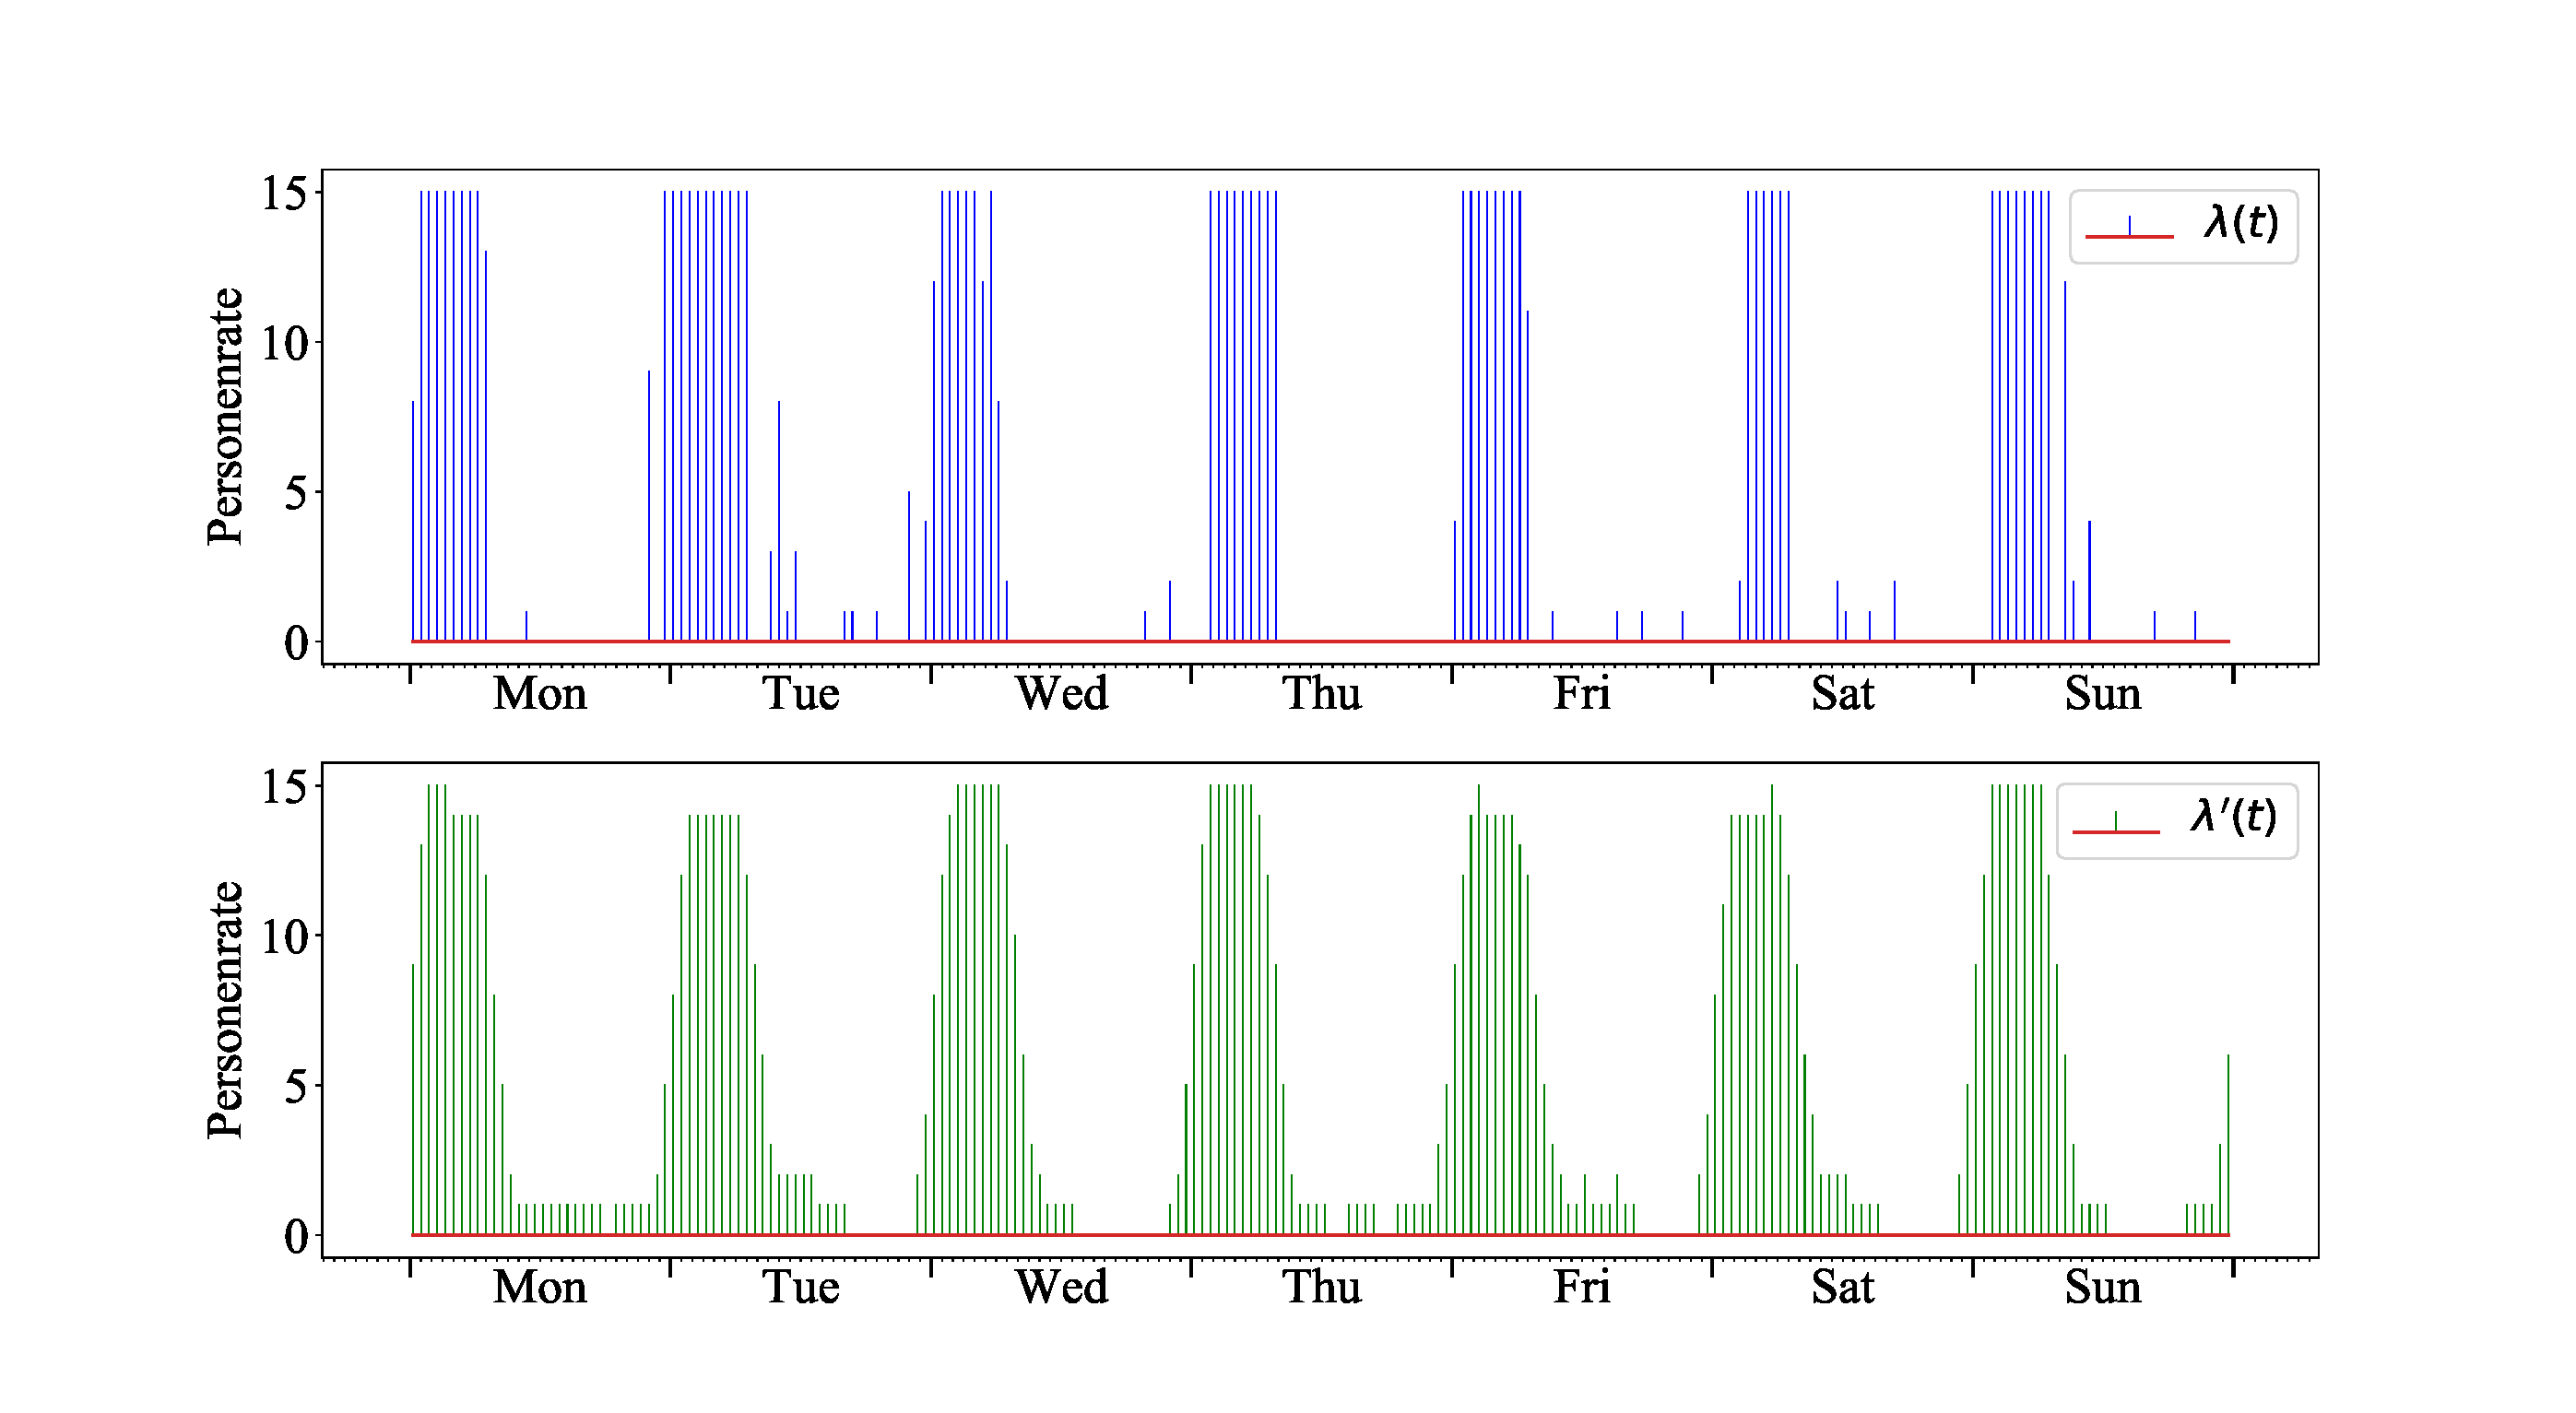
\includegraphics[width=\linewidth]{Abbildungen/evaluation/bin_size_influence_master_bedroom_float_900.pdf}
		\caption[Personenrate $\lambda (t)$ des Schlafzimmers bei einer Intervalldauer von  $\Delta t = \SI{600}{\second}$ und Approximation $\lambda '(t)$]{Personenrate $\lambda (t)$ des Schlafzimmers (Aruba-Datensatz) bei einer Intervalldauer von  $\Delta t = \SI{600}{\second}$ (oben) und Approximation $\lambda '(t)$ (unten)}
		\label{fig.bin_size_influence_master_bedroom_float_900}
	\end{center}
\end{figure}

Die Personenraten $\lambda(t)$ des Gästeschlafzimmers mit einer Intervalldauer von $\Delta t = \SI{600}{\second}$ sind in \bild{bin_size_influence_second_bedroom_float_600.pdf} aufgezeichnet. Die beste Approximation $\lambda ' (t)$ wird hierbei mit einer Ordnung von $l_\ind{opt} = 0$, also dem statischen Modell, erreicht. Die Prädiktion lautet für alle Intervalle $\lambda_\ind{stat} ' (t) = 0$. Der Prädiktionsfehler  beträgt $\epsilon_\ind{p} = 1.39$. 

\begin{figure}[!h]
	\begin{center}
		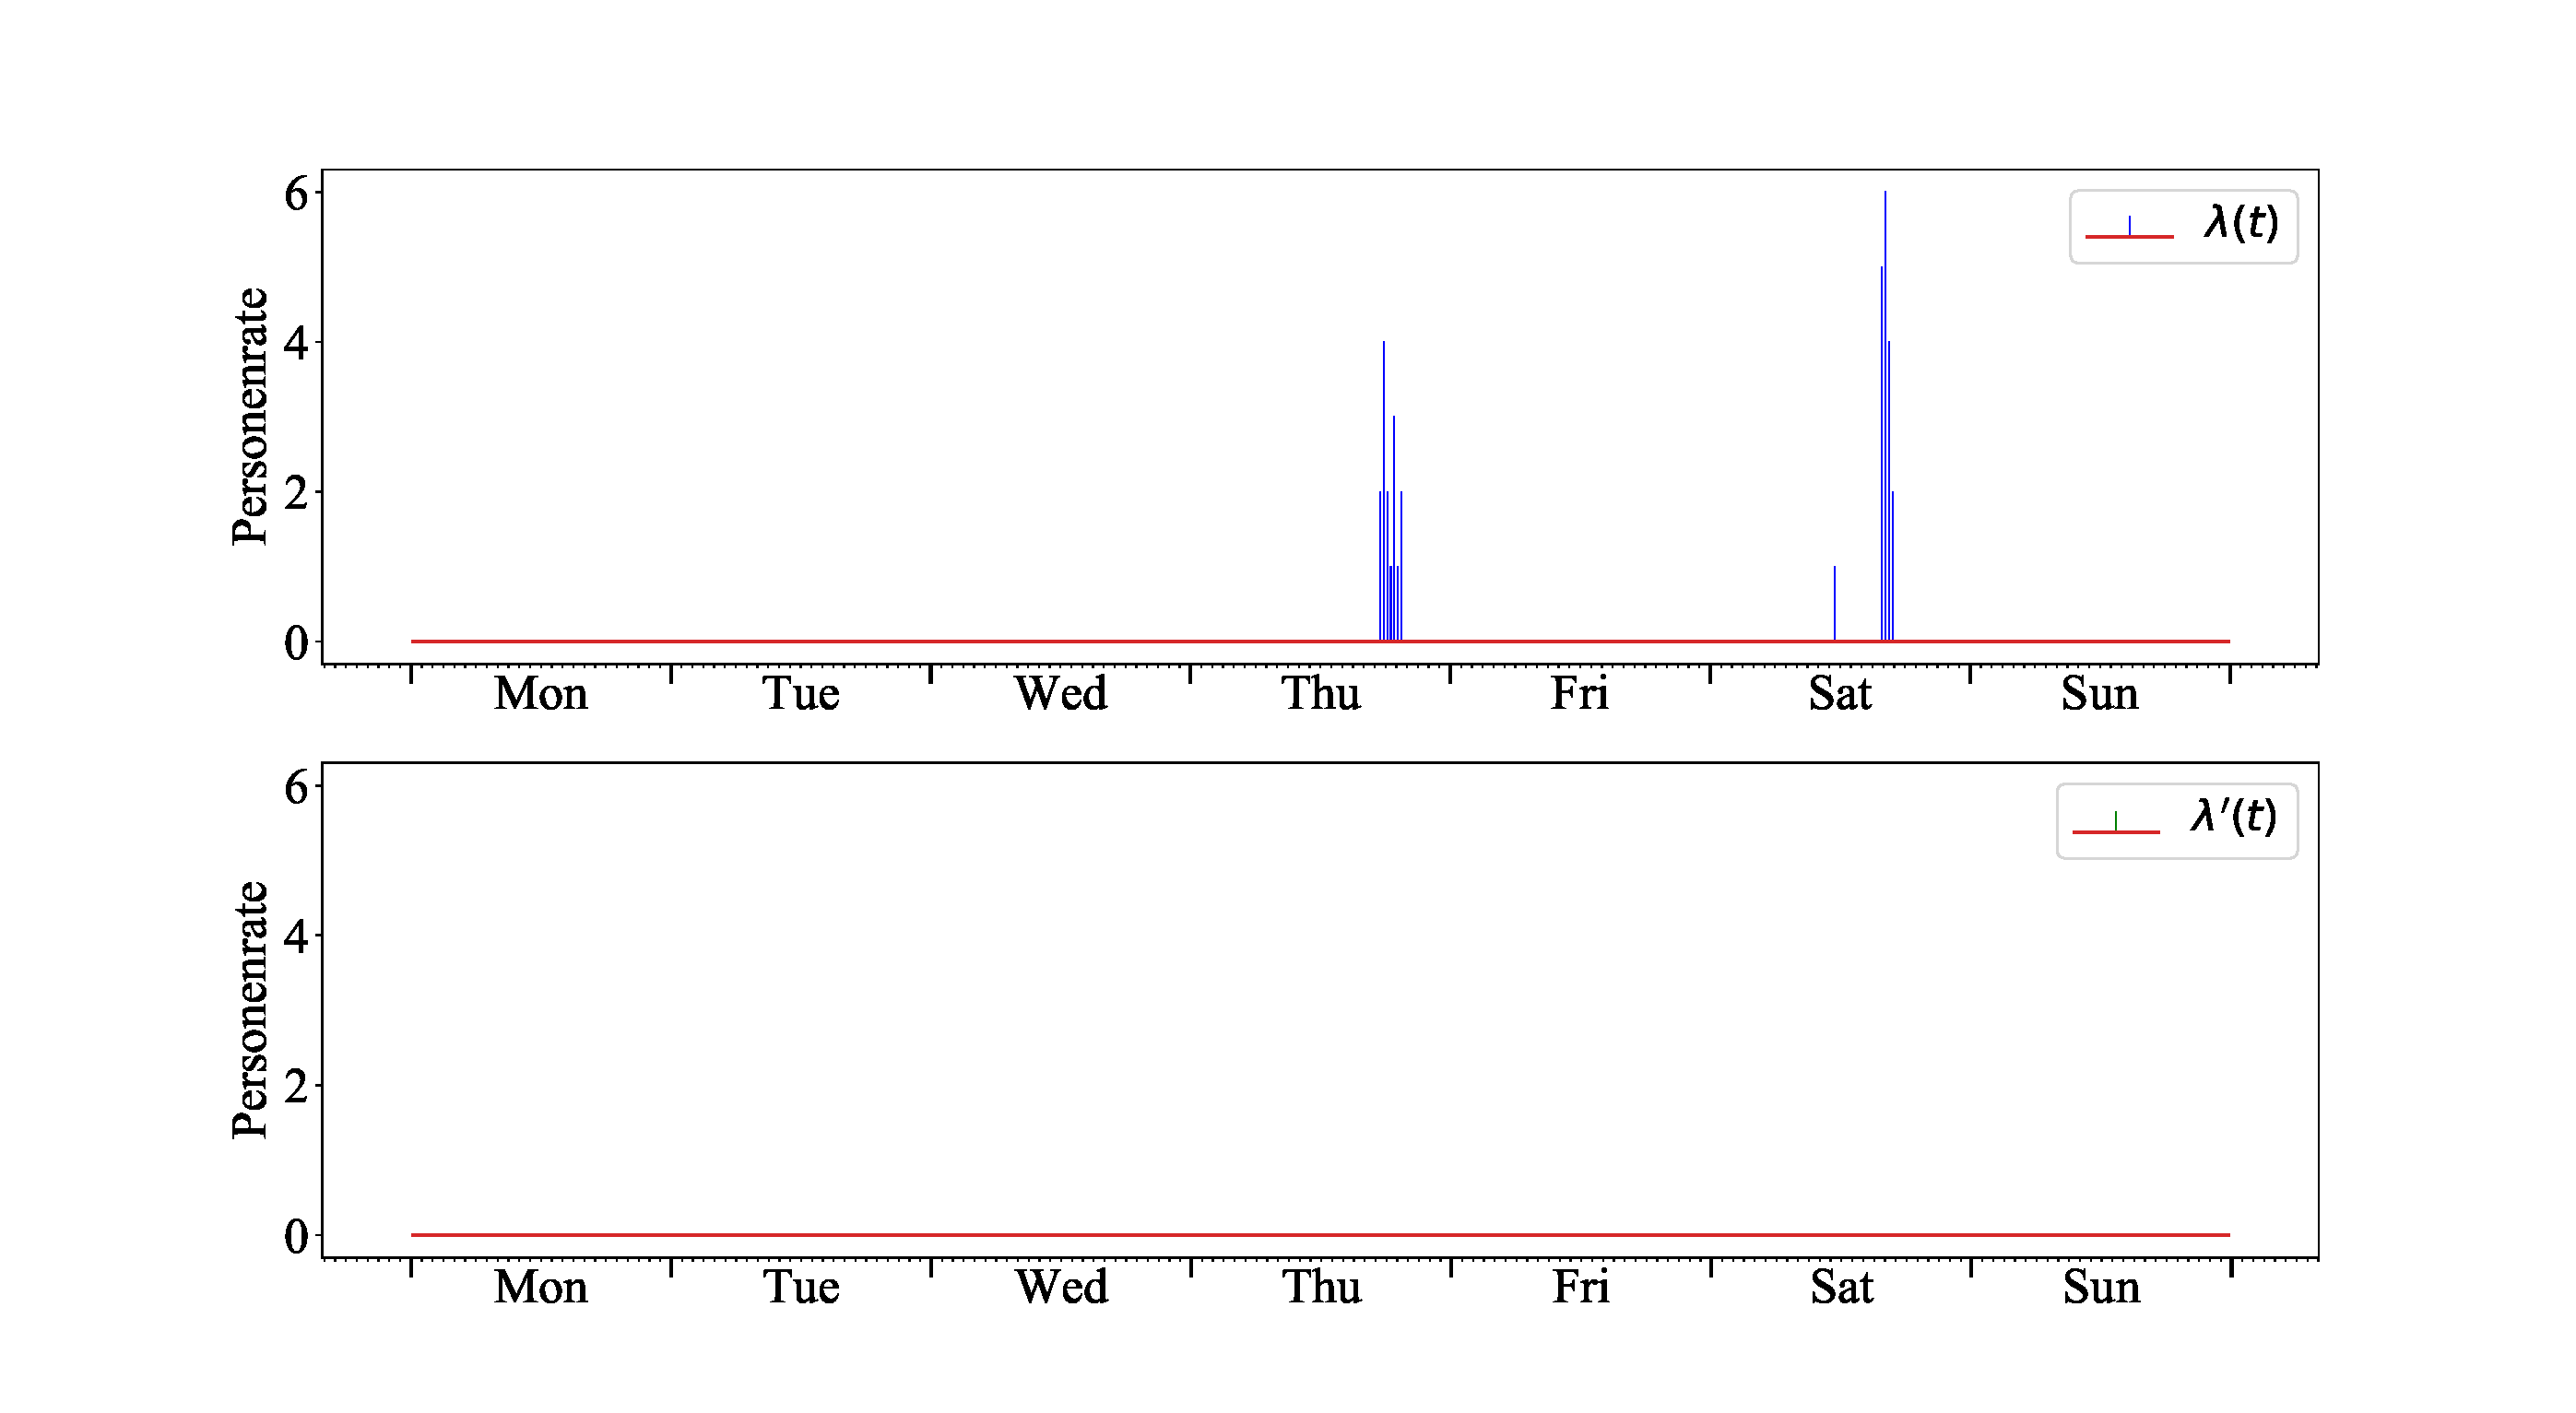
\includegraphics[width=\linewidth]{Abbildungen/evaluation/bin_size_influence_second_bedroom_float_600.pdf}
		\caption[Personenrate $\lambda (t)$ des Gästeschlafzimmers bei einer Intervalldauer von  $\Delta t = \SI{600}{\second}$ und Approximation $\lambda '(t)$]{Personenrate $\lambda (t)$ des Gästeschlafzimmers (Aruba-Datensatz) bei einer Intervalldauer von  $\Delta t = \SI{600}{\second}$ (oben) und Approximation $\lambda '(t)$ (unten)}
		\label{fig.bin_size_influence_second_bedroom_float_600.pdf}
	\end{center}
\end{figure}

Die untere Grafik von \bild{bin_size_influence_second_bedroom_float_900.pdf} veranschaulicht $\lambda (t)$ bei einer Intervalldauer von $\Delta t = \SI{900}{\second}$. Die beste Approximation wird in diesem Fall ebenfalls mit einer Modellordnung von $l_\ind{opt}=0$, also dem statischen Modell mit $\lambda_\ind{stat} ' (t) = \mathrm{const}.$ , erreicht. Die Prädiktion lautet nun für alle Intervalle $\lambda_\ind{stat} '(t) = 1$. Dies ist dadurch zu begründen, dass die durchschnittliche Personenrate bei größerer Intervalldauer steigt, und somit im Gegensatz zu \bild{bin_size_influence_second_bedroom_float_600.pdf} auf die nach Gleichung \ref{eq:Personenraten-Funktion} nächstgelegene natürliche Zahl gerundet wird, welche in diesem Fall 1 beträgt.

\begin{figure}[!h]
	\begin{center}
		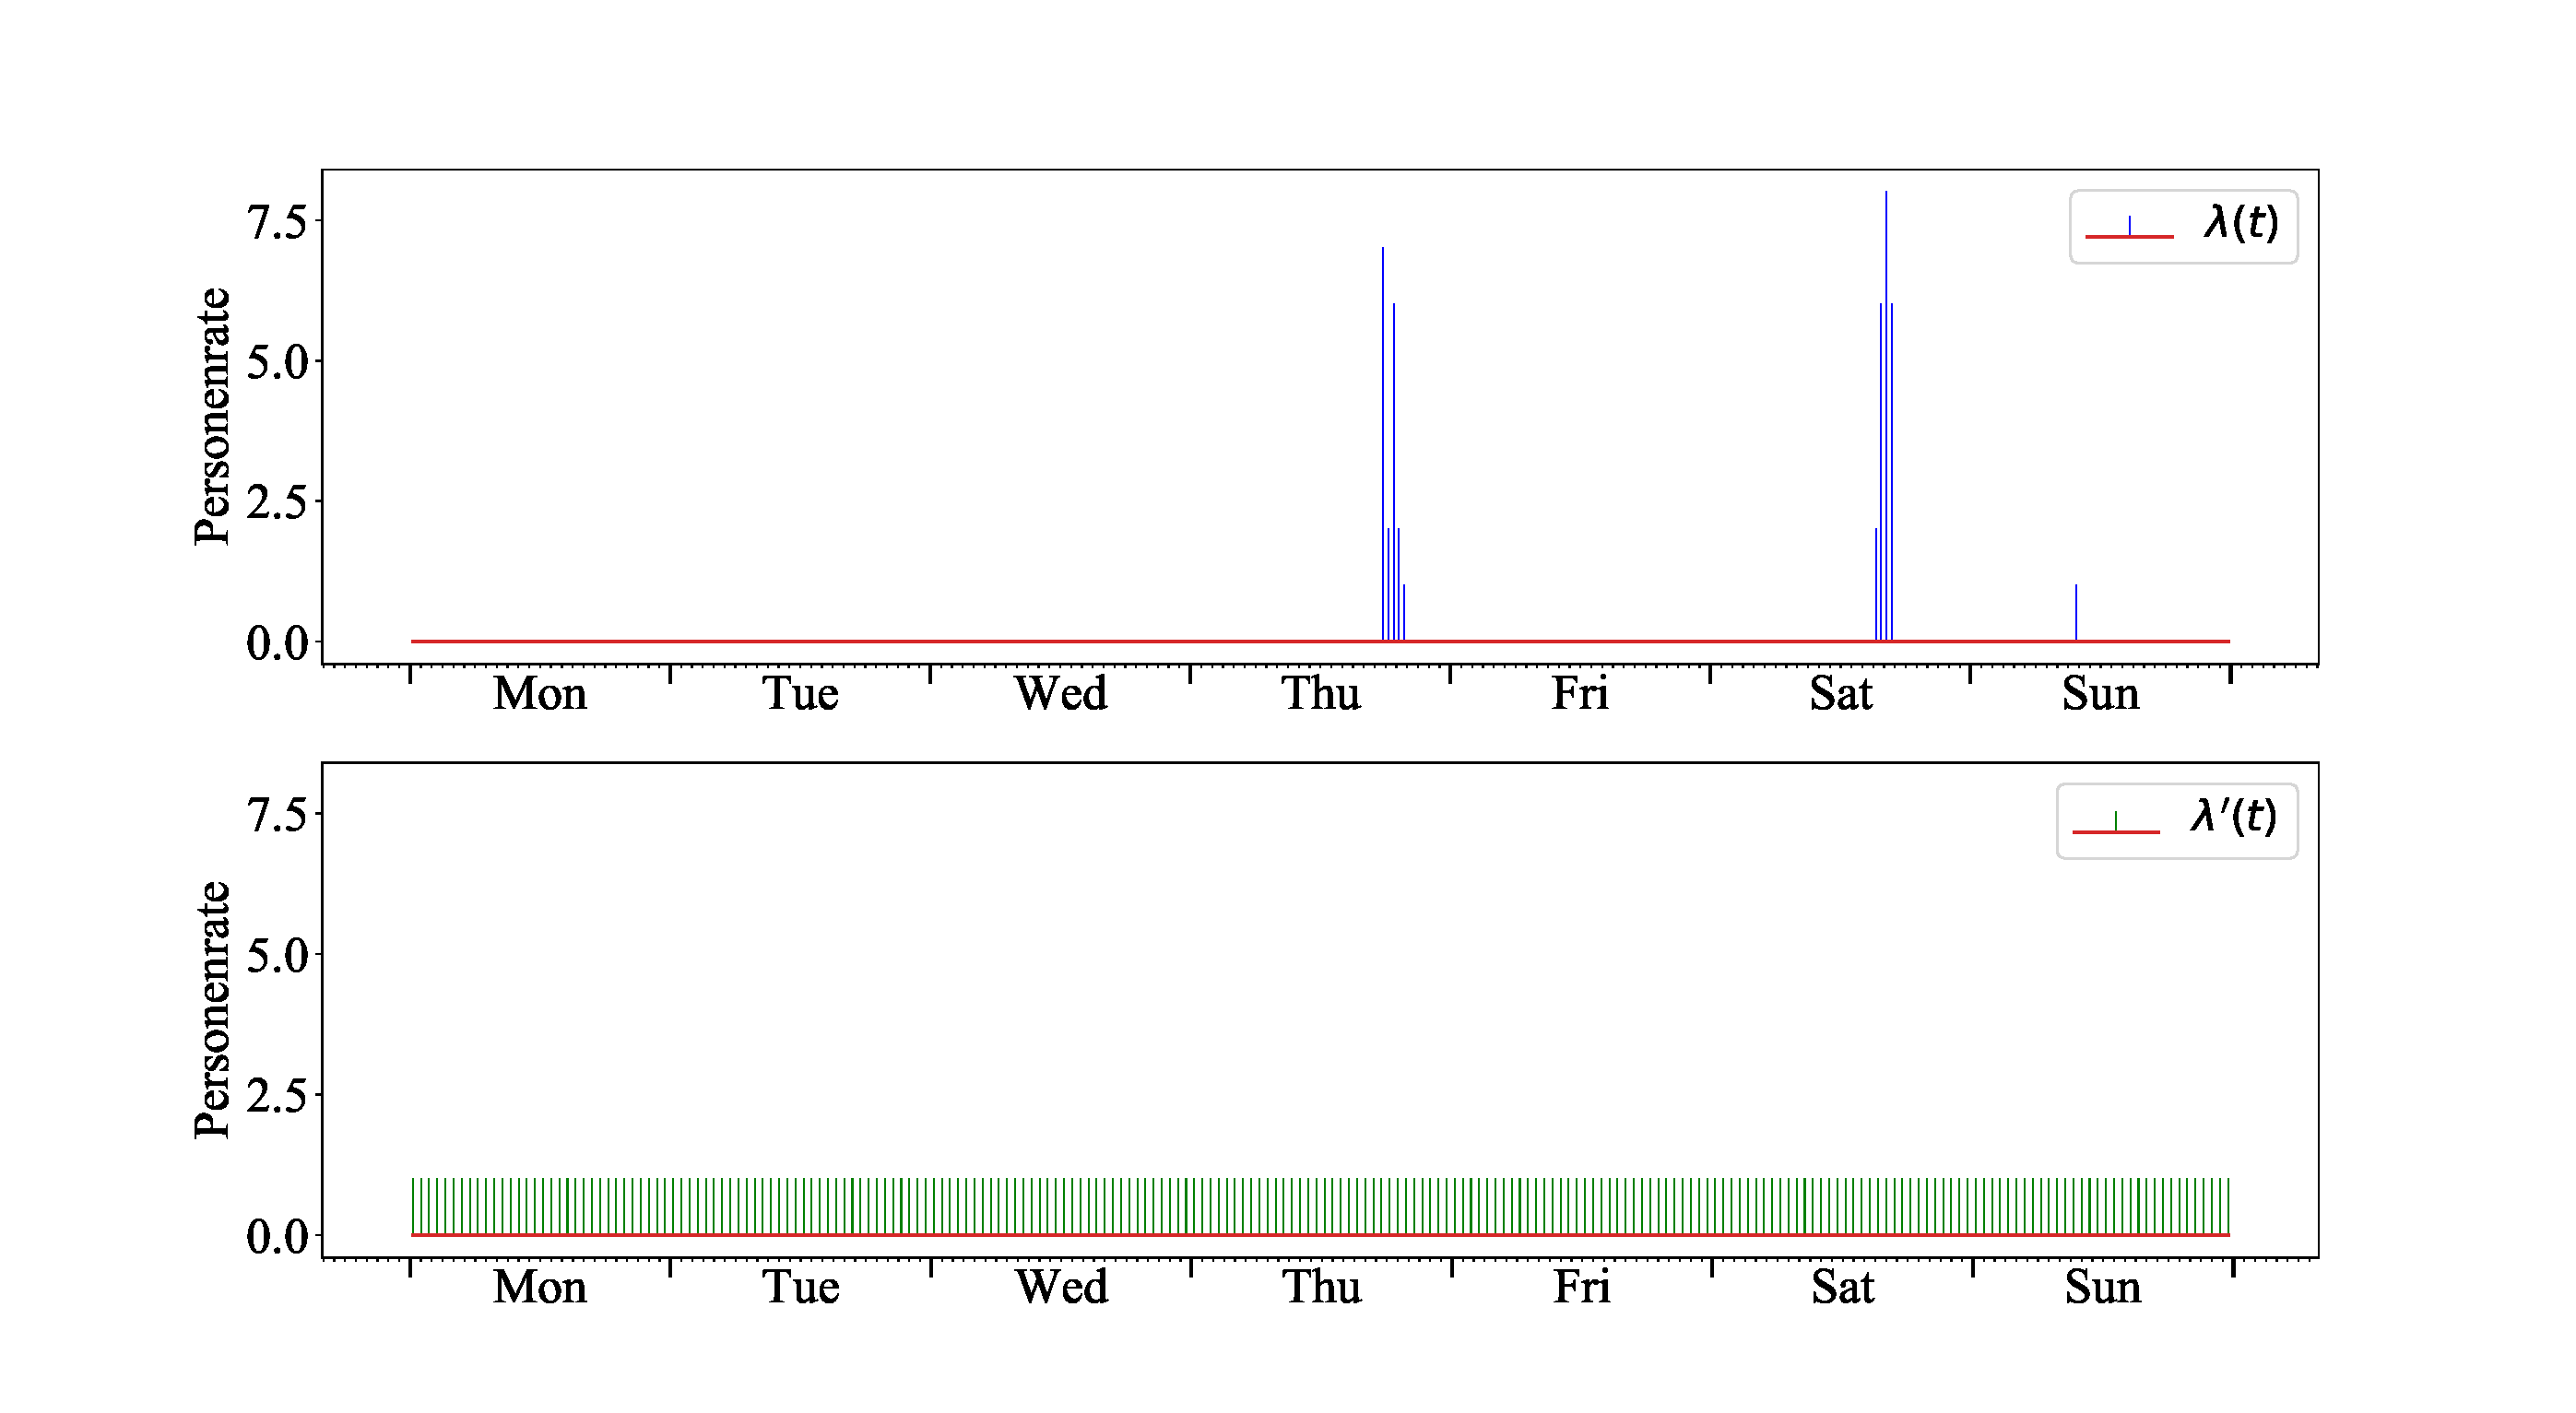
\includegraphics[width=\linewidth]{Abbildungen/evaluation/bin_size_influence_second_bedroom_float_900.pdf}
		\caption[Personenrate $\lambda (t)$ des Gästeschlafzimmers bei einer Intervalldauer von  $\Delta t = \SI{600}{\second}$ und Approximation $\lambda '(t)$]{Personenrate $\lambda (t)$ des Gästeschlafzimmers (Aruba-Datensatz) bei einer Intervalldauer von  $\Delta t = \SI{600}{\second}$ (oben) und Approximation $\lambda '(t)$ (unten)}
		\label{fig.bin_size_influence_second_bedroom_float_900.pdf}
	\end{center}
\end{figure}

Der Prädiktionsfehler  ergibt sich zu $\epsilon_\ind{p} = 2.04$. In Tabelle \ref{tab.Prädiktionsfehler aruba_float} sind die durchschnittlichen Prädiktionsfehler der Zellen des Datensatzes bei verschiedenen Intervalldauern aufgeführt. In die Fehlerermittlung flossen nur solche Zellen ein, bei denen in mindestens 5 \% der Intervalle eine Person detektiert worden ist. Unter Berücksichtigung dieser Voraussetzung wurden sieben der insgesamt zehn Räume bzw. Zellen des Aruba-Datensatzes zur Fehlerermittlung in Tabelle \ref{tab.Prädiktionsfehler aruba_float} genutzt.

\begin{table}[!h]
	\centering
	\caption{Prädiktionsfehler $\epsilon_\ind{p}$ bei unterschiedlichen Intervalldauern $\Delta t$ (Aruba)} \label{tab.Prädiktionsfehler aruba_float}
	\vspace*{-3mm}
	\begin{tabular}{lccr}
		\toprule
		Intervalldauer $\Delta t$		& $\epsilon_\ind{p,opt}$ & $\epsilon_\ind{p,stat}$  & Vergleich $\epsilon_\ind{p,opt}$ zu $\epsilon_\ind{p,stat}$              \\
		\midrule
		\SI{300}{\second}	& 1.17        & 1.43 & -18.18 \% \\
		\rowcolor{Snow2}
		\SI{600}{\second} 	& 2.23       & 2.76 & -19.20 \% \\
		\SI{900}{\second}			& 2.81        & 3.51 & -19.94 \% \\
		\bottomrule
	\end{tabular} 
\end{table}

Eine weitere Evaluation des Modells erfolgt anhand des UOL-Datensatzes. \bild{bin_size_influence_cell_row_23_col_25_float_600} zeigt die Personenraten $\lambda (t)$ bei einer Intervalldauer von $\Delta t = \SI{600}{\second}$ sowie die Prädiktion $\lambda ' (t) $ der optimalen Modellordnung $l_\ind{opt} = 2$ mit einem Prädiktionsfehler von $\epsilon_\ind{p,opt} = 11.38$.
% Hier Abbildung bin_size_influence_cell_row_23_col_25_float_600.pdf einfügen
\begin{figure}[!h]
	\centering
	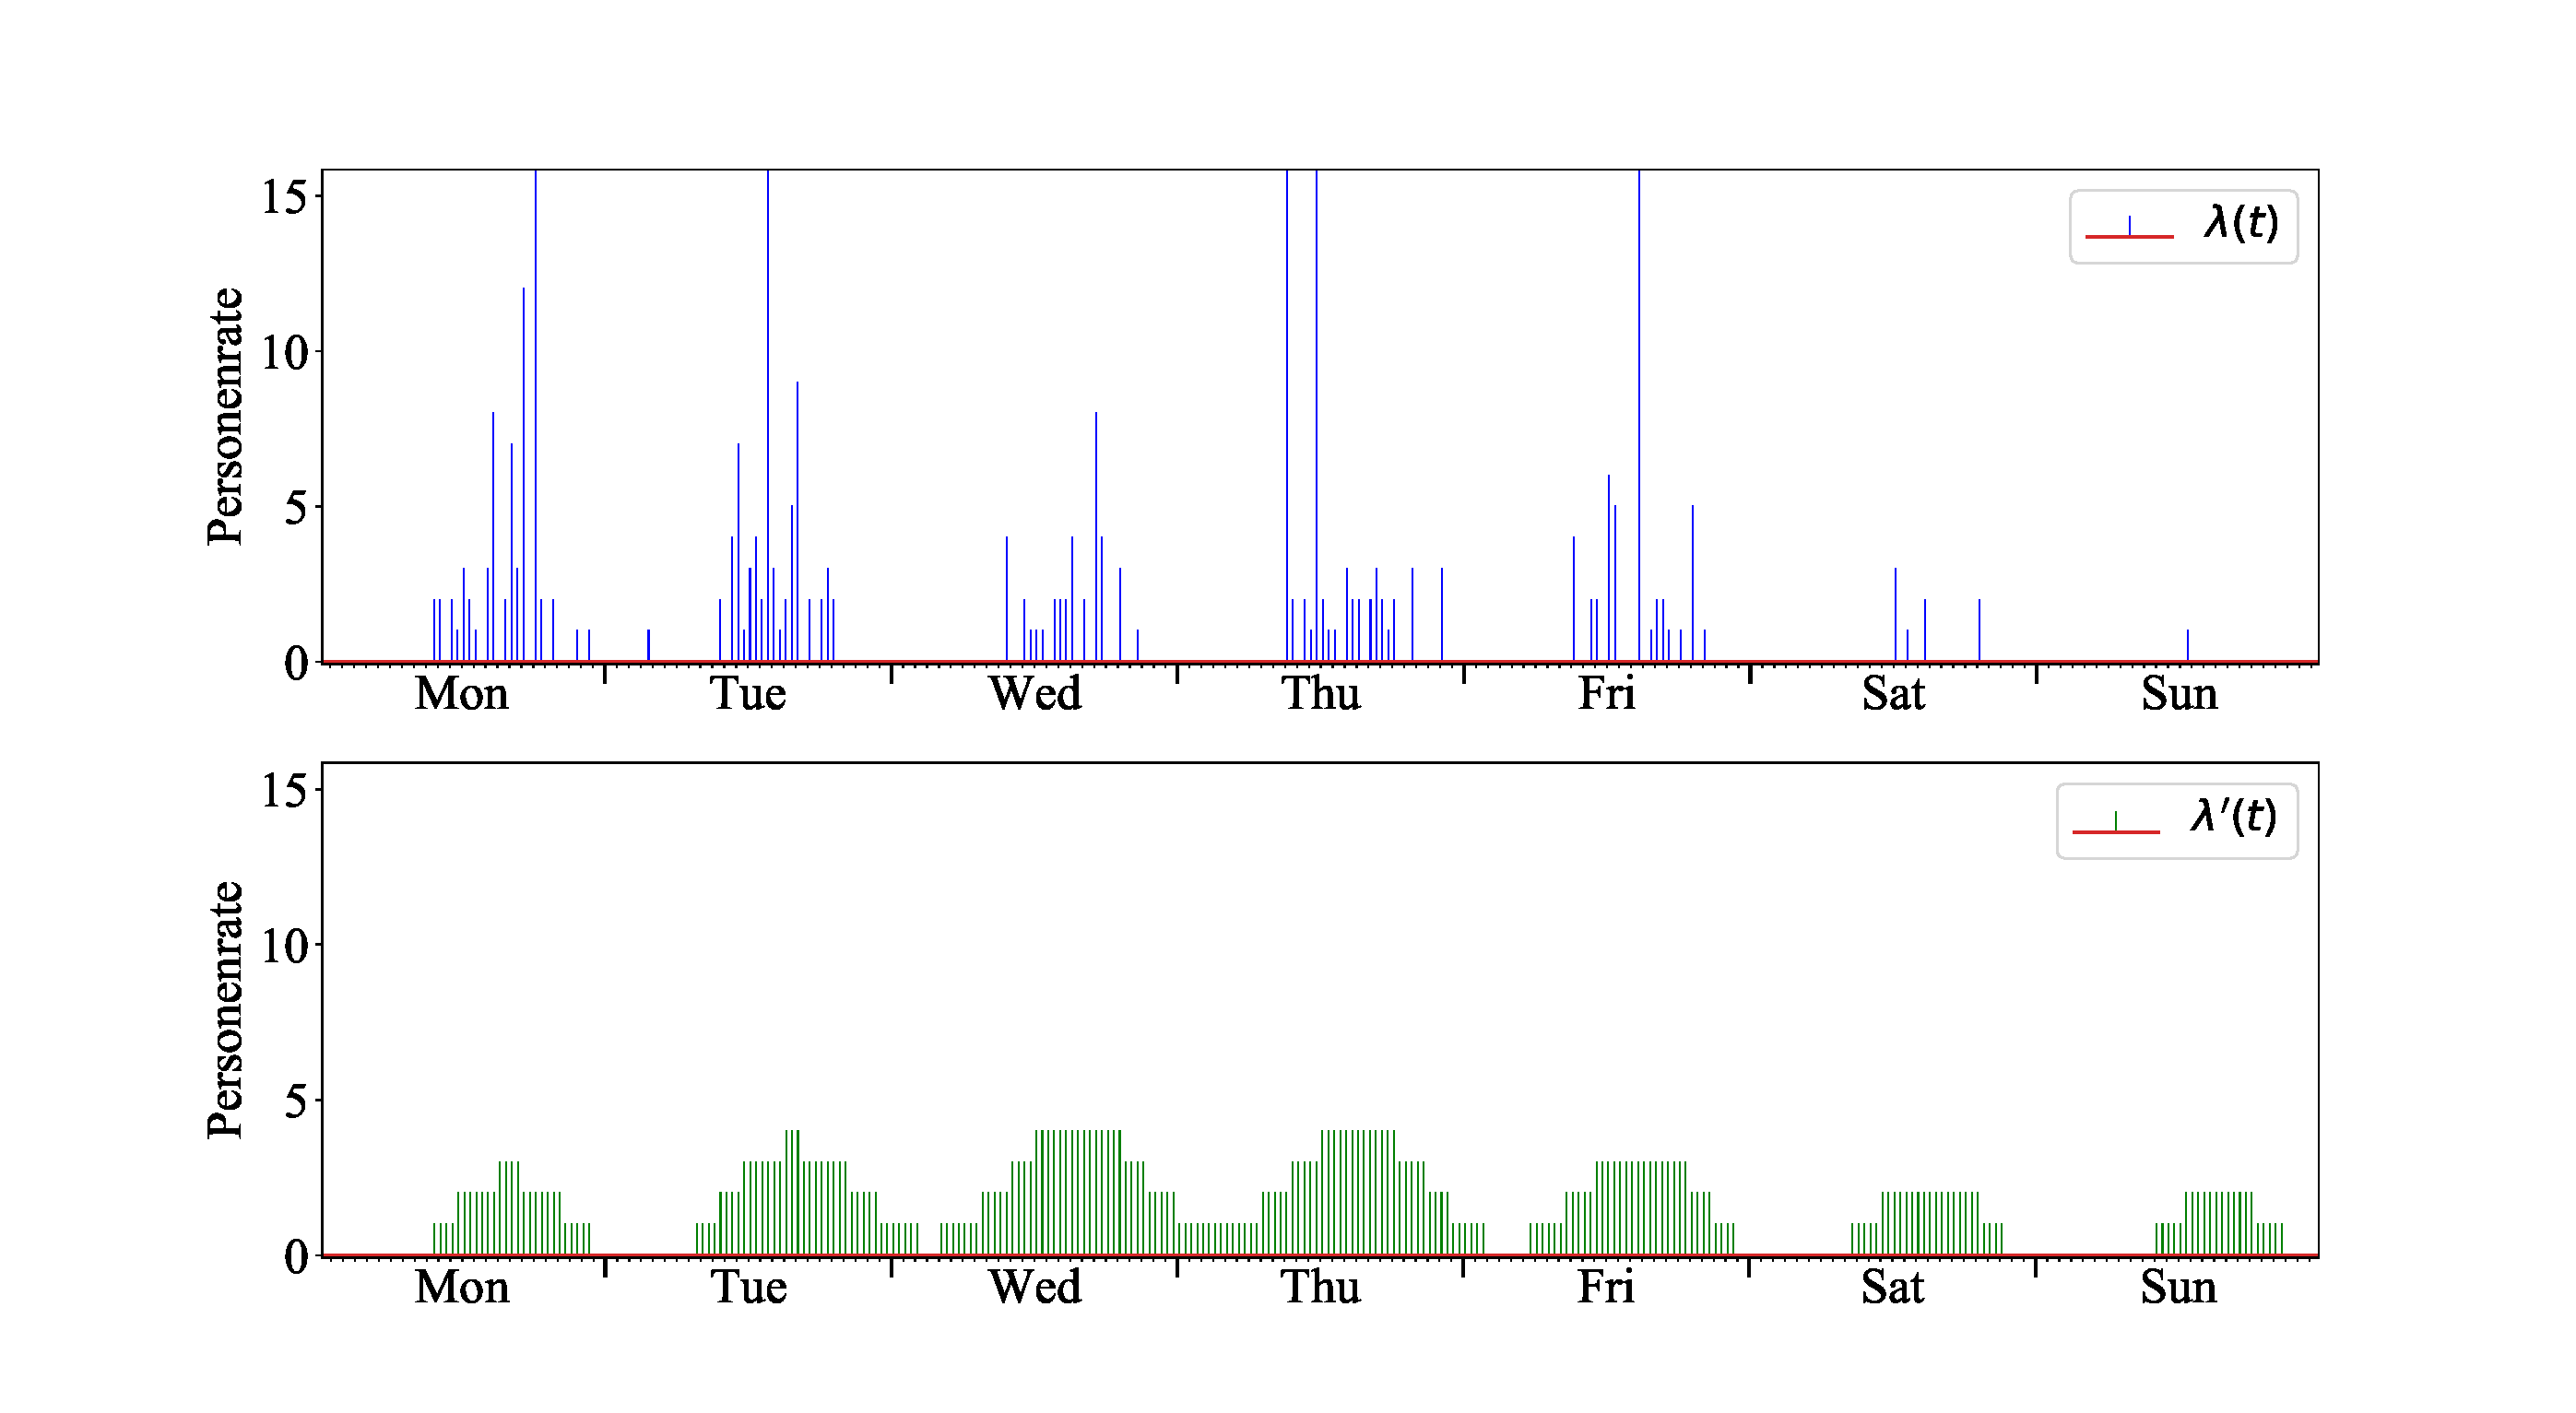
\includegraphics[width=1.0\linewidth]{Abbildungen/evaluation/bin_size_influence_cell_row_23_col_25_float_600}
	\caption{Personenraten einer Beispielzelle des UOL Datensatzes bei einer Intervalldauer von $\Delta t = \SI{600}{\second}$ mit optimaler Modellordnung}
	\label{fig.bin_size_influence_cell_row_23_col_25_float_600}
\end{figure}

Dieser, im Vergleich zu dem quantitativen Modell des Aruba-Datensatzes, hohe Fehler, lässt sich durch die höhere Varianz der einzelnen Wochen innerhalb des UOL-Datensatzes erklären. Jedoch lassen sich auch hier der Tag-Nacht-Rhythmus sowie ein Abflachen der Personenraten während der beiden Wochenendtage erkennen. Die Annahme einer statischen Personenrate von $\lambda_\ind{stat} ' (t) = \mathrm{const}. = 1 $ resultiert in einem Prädiktionsfehler von $\epsilon_\ind{p,stat} = 11.46$. Im Vergleich zum statischen Modell kann also mit einer Modellordnung von $l_\ind{opt} = 2$ eine Verbesserung um 0.7 \% erreicht werden.

Das Modell bei einer Intervalldauer von $\Delta t = \SI{900}{\second}$ ist in \bild{bin_size_influence_cell_row_23_col_25_float_900} dargestellt. 
% Hier Abbildung bin_size_influence_cell_row_23_col_25_float_900.pdf einfügen
\begin{figure}[!h]
	\centering
	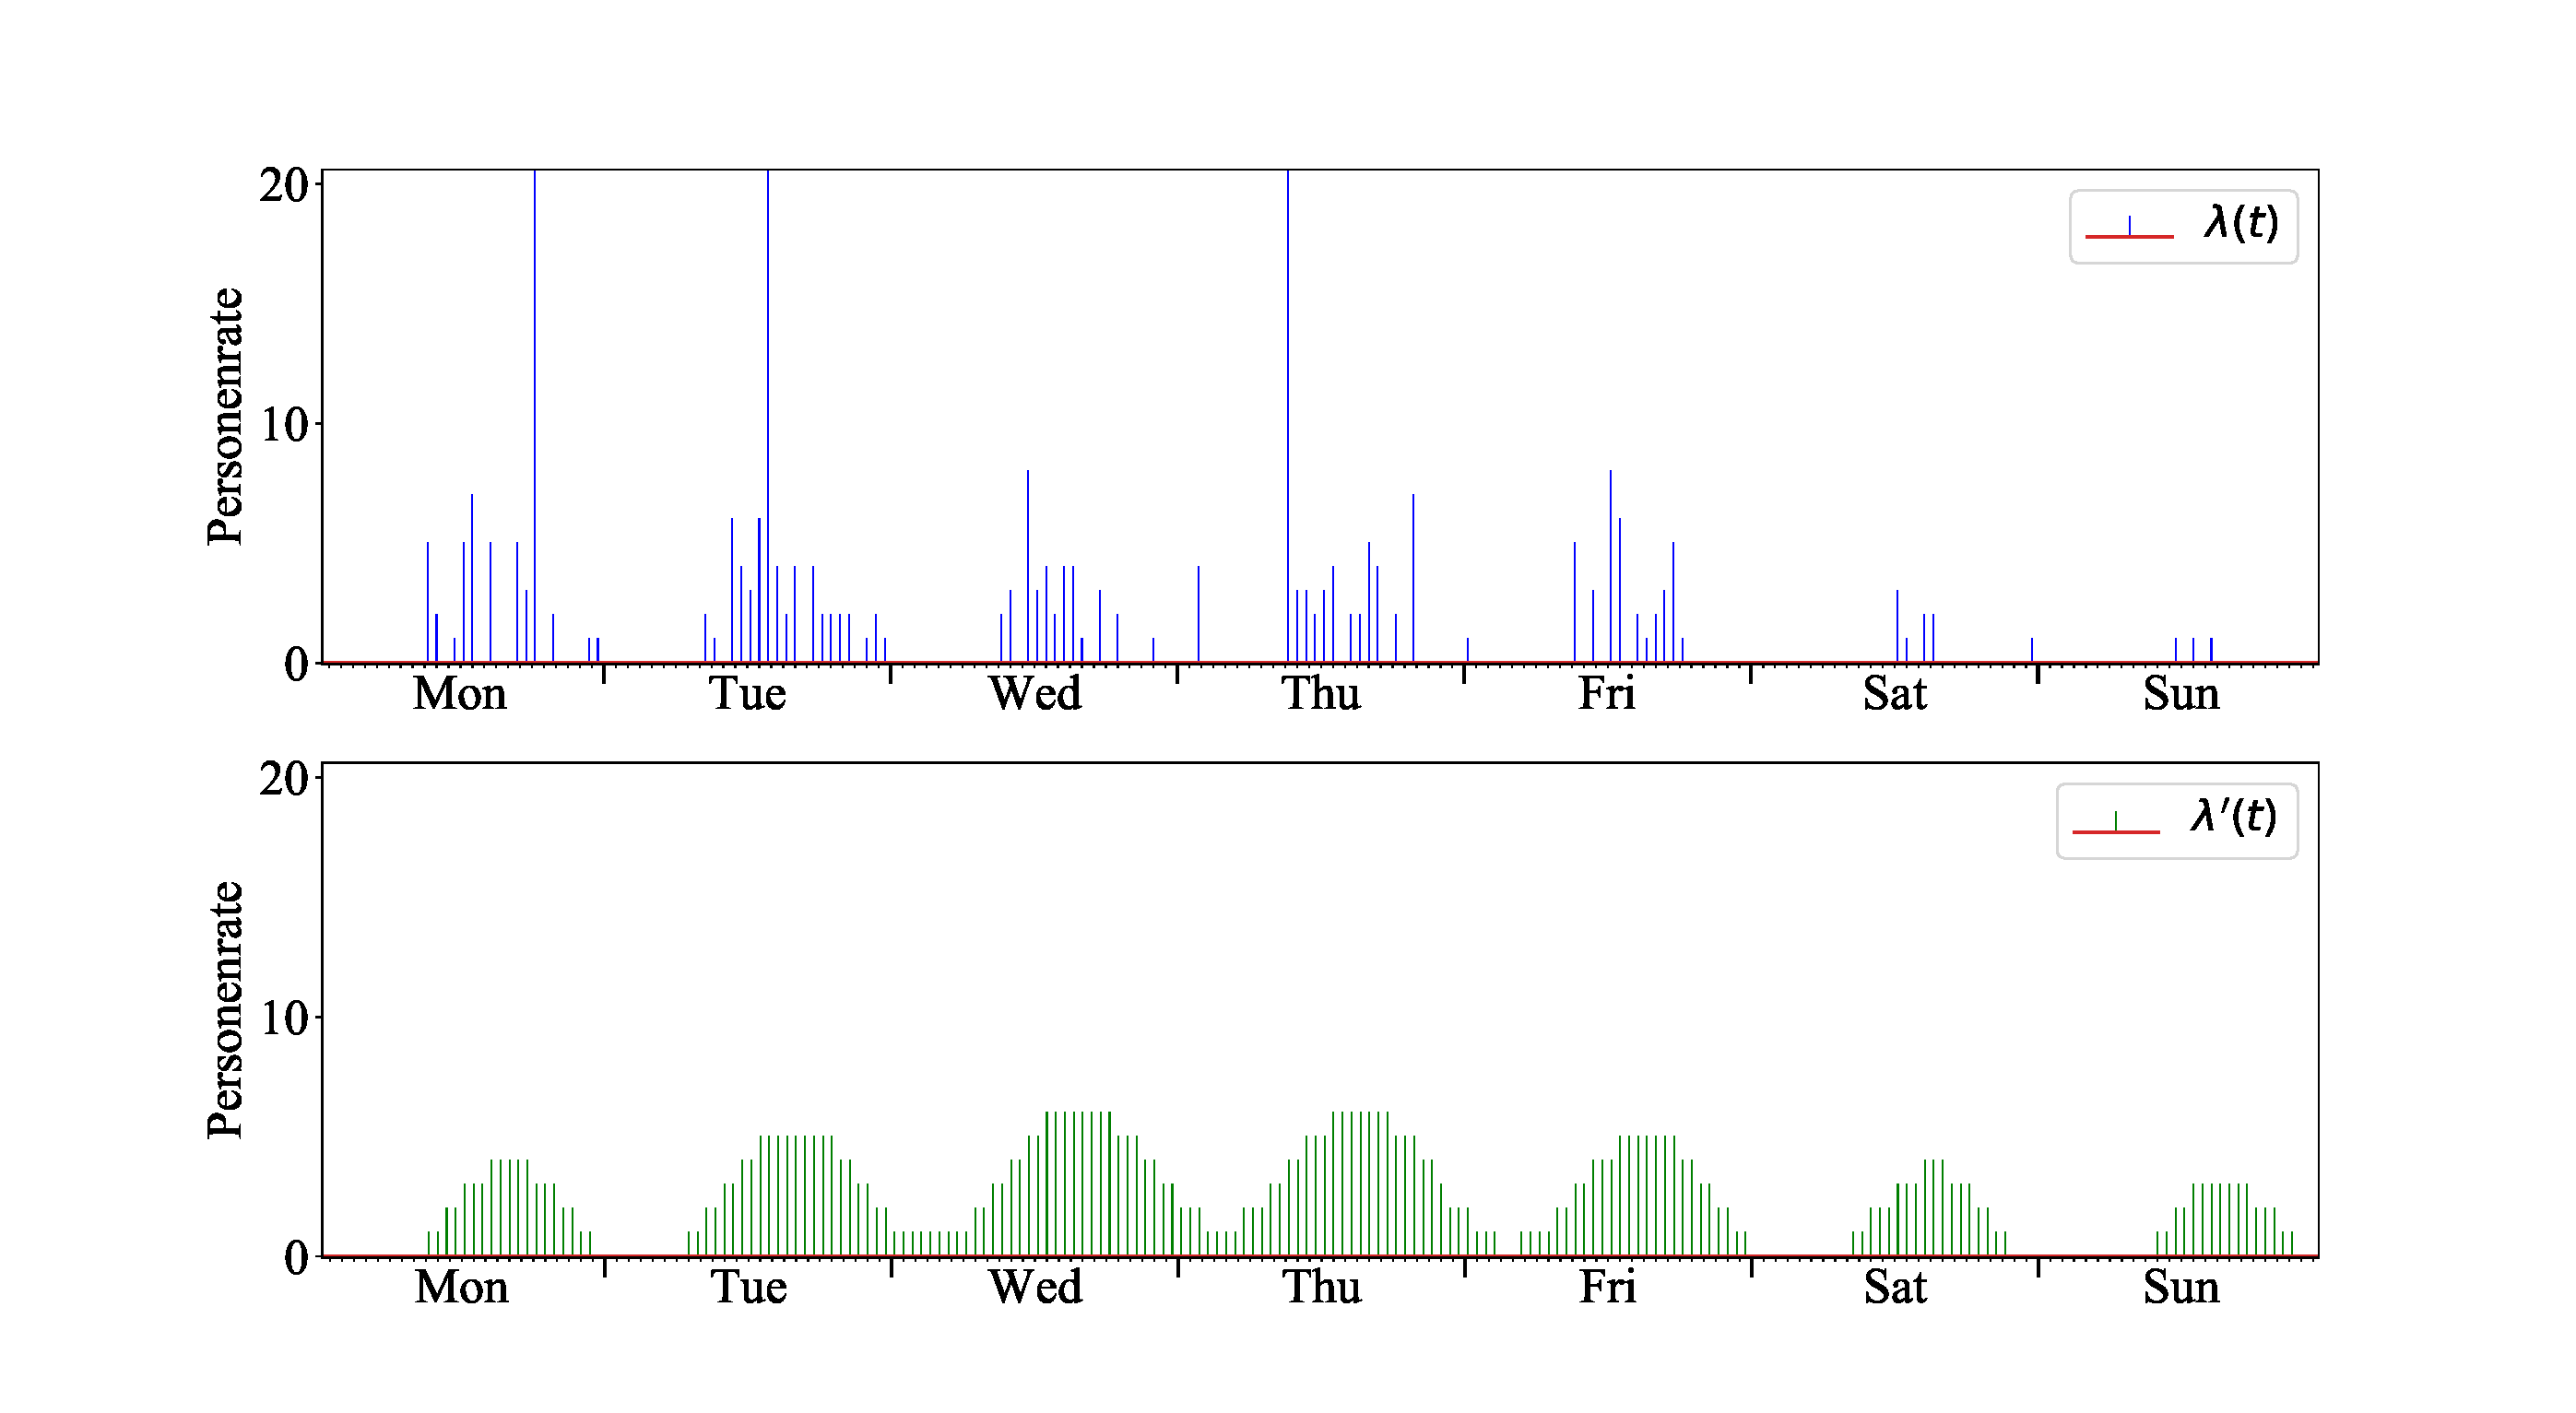
\includegraphics[width=1.0\linewidth]{Abbildungen/evaluation/bin_size_influence_cell_row_23_col_25_float_900}
	\caption{Personenraten einer Beispielzelle des UOL Datensatzes bei einer Intervalldauer von $\Delta t = \SI{900}{\second}$ mit optimaler Modellordnung}
	\label{fig.bin_size_influence_cell_row_23_col_25_float_900}
\end{figure}

Zu erkennen ist, dass die Personenraten $\lambda (t)$ im Vergleich zu \bild{bin_size_influence_cell_row_23_col_25_float_600} höher liegen. Dies ist erneut durch die längere Intervalldauer $\Delta t$ zu erklären. Für $\Delta t = \SI{900}{\second}$ liegt die optimale Modellordnung ebenfalls bei $l_\ind{opt} = 2$, mit einem Prädiktionsfehler von $\epsilon_\ind{p,opt} = 14.51$. Im Vergleich dazu liegt der Prädiktionsfehler des statischen Modells bei $\epsilon_\ind{p,stat} = 14.65$, es konnte also eine Verbesserung um 0.95 \% erreicht werden. \\
In Tabelle \ref{tab.Prädiktionsfehler uol_float} sind die durchschnittlichen Prädiktionsfehler der Zellen des Datensatzes bei verschiedenen Intervalldauern aufgeführt.

\begin{table}[!h]
	\centering
	\caption{Prädiktionsfehler $\epsilon_\ind{p}$ bei unterschiedlichen Intervalldauern  $\Delta t$ (UOL)}\label{tab.Prädiktionsfehler uol_float}
	\vspace*{-3mm}
	\begin{tabular}{lccr}
		\toprule
		Intervalldauer $\Delta t$		& $\epsilon_\ind{p,opt}$	&  $\epsilon_\ind{p,stat}$  & Vergleich $\epsilon_\ind{p,opt}$ zu $\epsilon_\ind{p,stat}$              \\
		\midrule
		\SI{300}{\second}	& 4.80           & 4.83 & -0.63 \% \\
		\rowcolor{Snow2}
		\SI{600}{\second} 	& 6.38           & 6.44 & -0.93 \% \\
		\SI{900}{\second}			& 6.91           & 6.99 & -1.15 \% \\
		\bottomrule
	\end{tabular} 
\end{table}
Verglichen werden erneut die Fehler $\epsilon_\ind{p,opt}$ der Modelle mit einer optimalen Modellordung, demgegenüber gestellt sind die Prädiktionsfehler $\epsilon_\ind{p,stat}$ der statischen Modelle. In die Fehlerermittlung flossen nur Zellen ein, bei welchen in mindestens 5 \% der Intervalle Personendetektionen vorliegen. Unter Berücksichtigung dieser Voraussetzung wurden 205 der insgesamt 3060 Zellen des UOL-Datensatzes zur Fehlermittlung in Tabelle \ref{tab.Prädiktionsfehler uol_float} genutzt. \\
\newpage
Eine Darstellung des über die Umgebung $\mathcal{U}$ gelegten Gitters mit seinen einzelnen Zellen bietet \bild{original_float_data}. Für ein beispielhaftes Zeitintervall $\Delta t_i$ mit einer Dauer von $\Delta t = \SI{600}{\second}$ ist hier für jede Zelle die zugehörige Personenrate $\lambda (t)$ farblich dargestellt. Die entsprechenden Werte der Personenraten $\lambda (t)$ sind farblich kodiert und können der eingezeichneten Farbskala entnommen werden. Zu erkennen ist, dass im vorliegenden Zeitintervall die höchsten Personenraten $\lambda (t)$ innerhalb des linken, oberen Bereiches des Bürogebäudes vorzufinden sind. Außerhalb des Gebäudes finden sich vereinzelt Bereiche mit niedrigen Personenraten (vgl. \bild{original_float_data}).
% caption ändern !
\begin{figure}[!h]
	\centering
	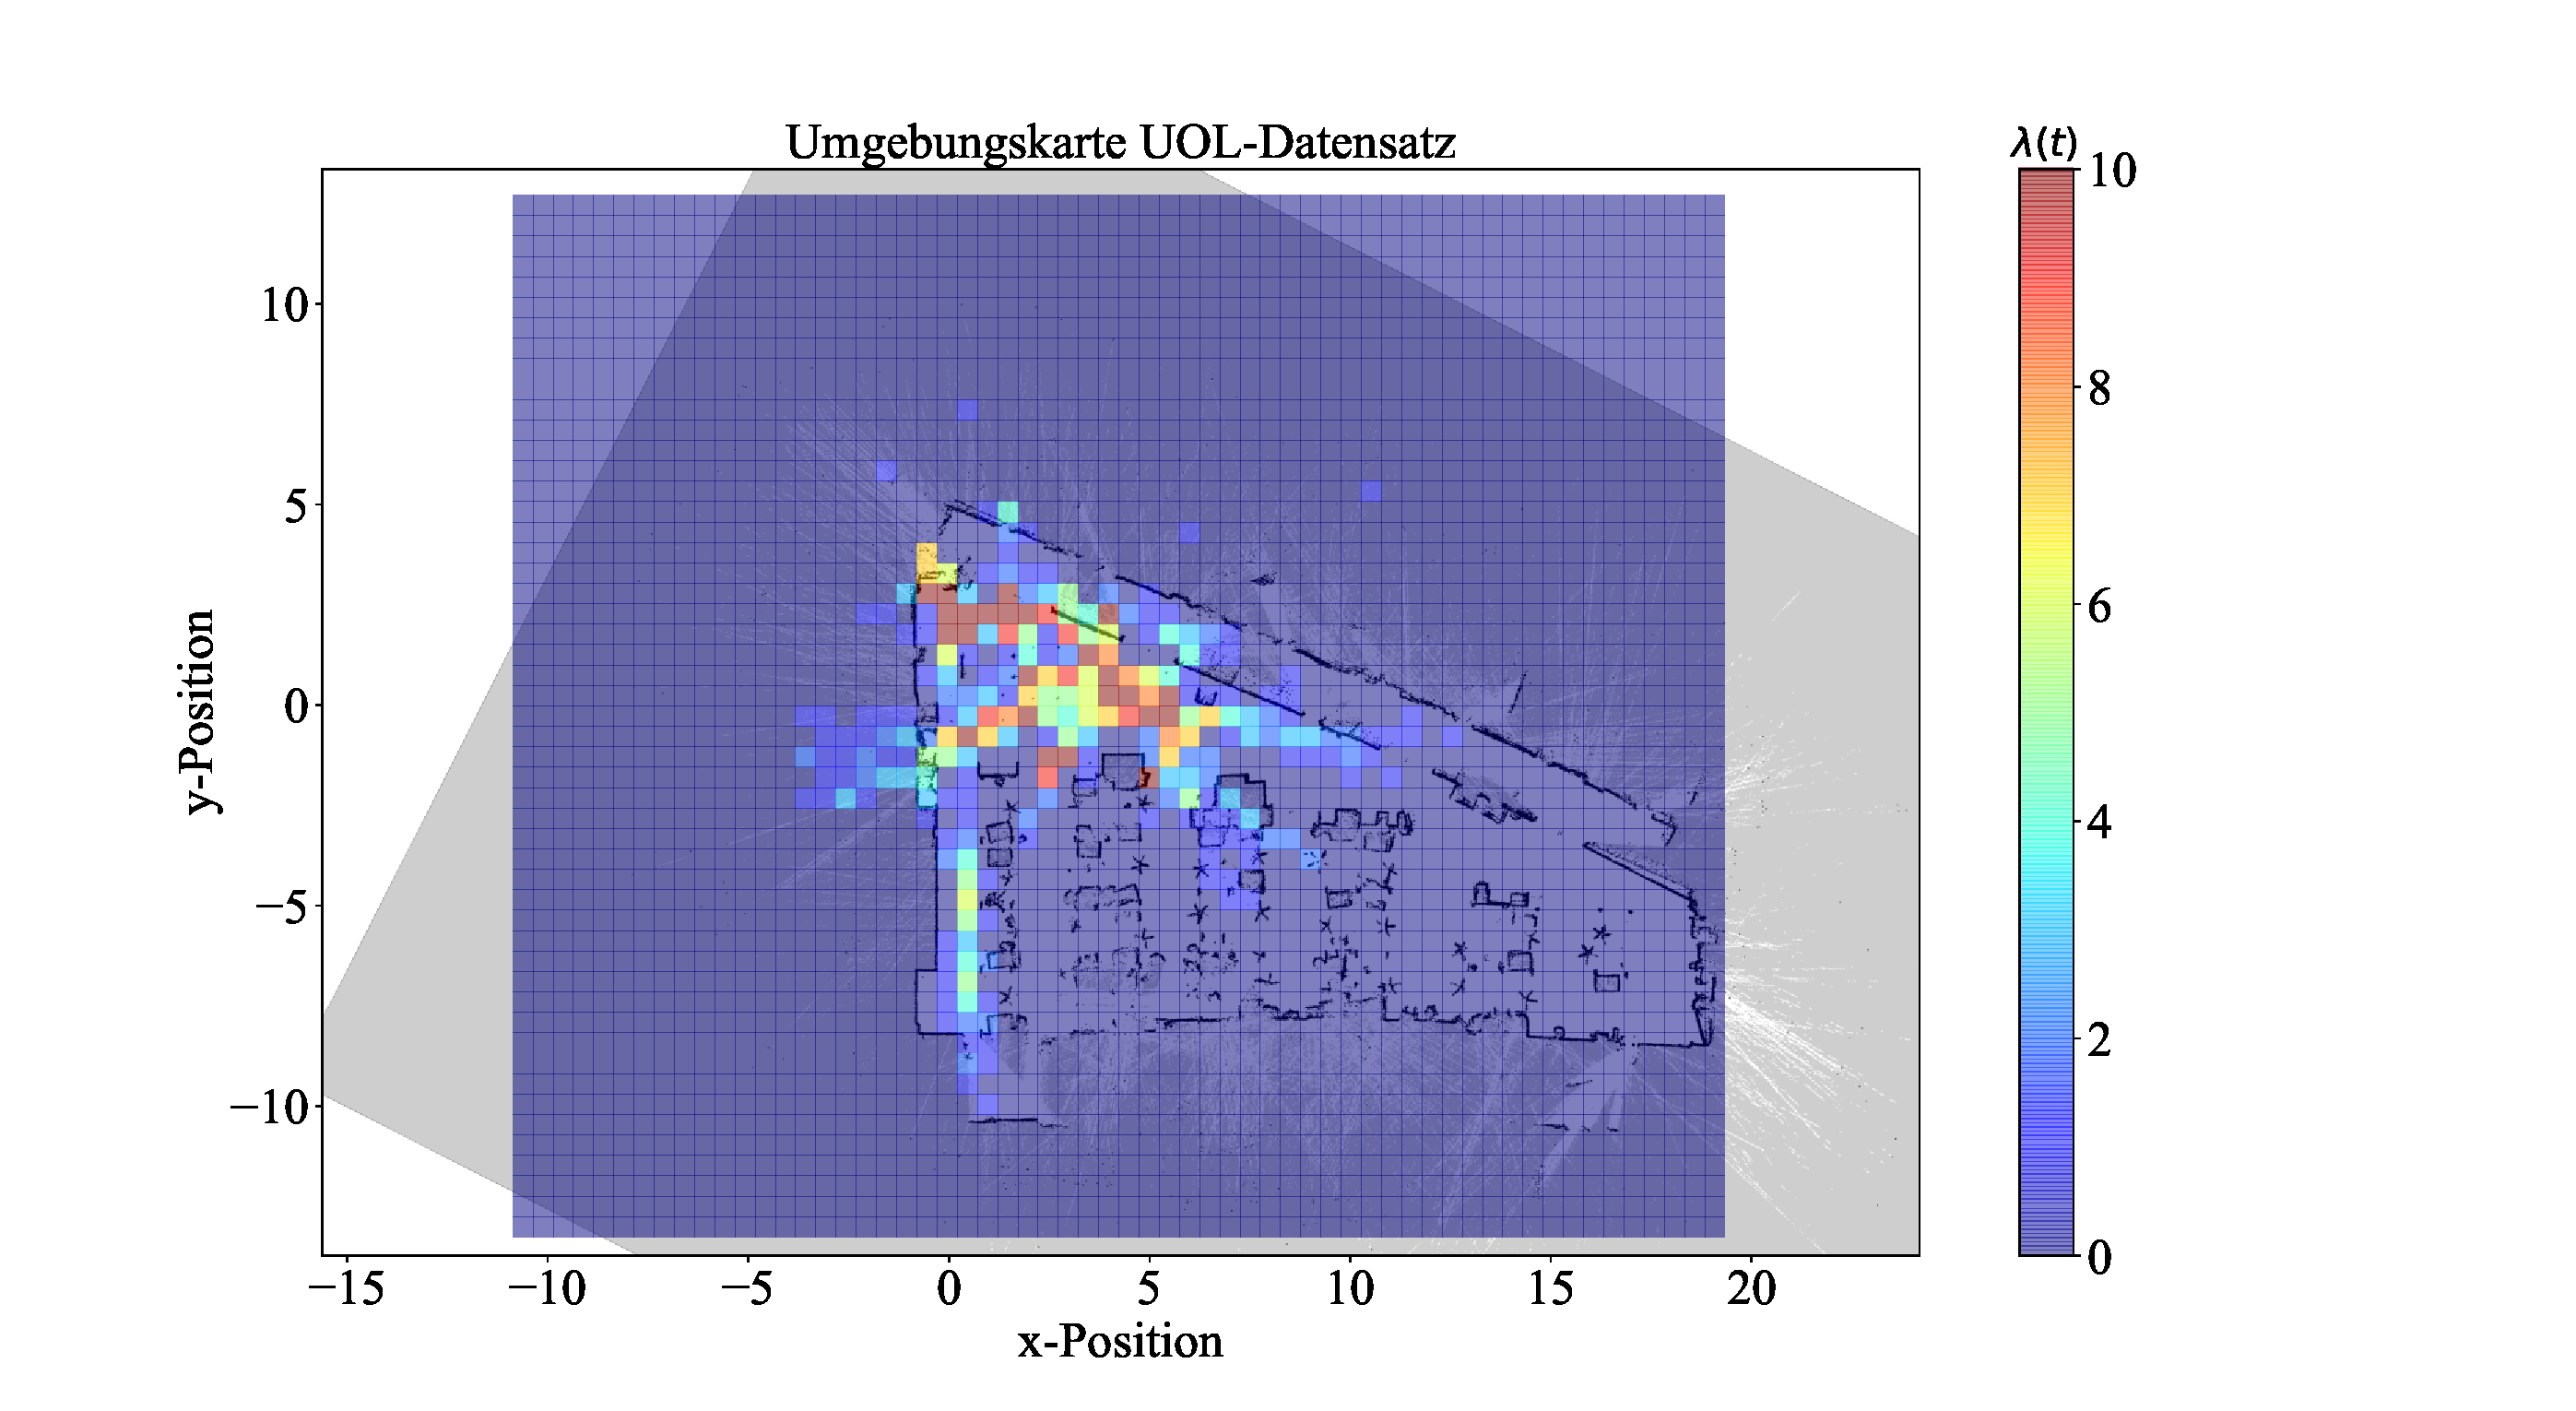
\includegraphics[width=1.0\linewidth]{Abbildungen/evaluation/original_float_data}
	\caption{Tatsächliche Personenraten $\lambda(t)$ innerhalb eines Beispielintervalls $\Delta t_i$}
	\label{fig.original_float_data}
\end{figure}

Ein grafischer Vergleich zwischen den mittels der optimalen Modellordnungen $l_\ind{opt}$ berechneten FreMEn-Modellen und den statischen Modellen der Personenraten $\lambda (t)$ kann mit Hilfe von \bild{float_fremen_vs_static} gezogen werden. \\

\begin{figure}[!h]
	\centering
	\subfigure[Prognostizierte Personenraten $\lambda'(t)$ mit FreMEn-Modellen der Ordnungen $l_\ind{opt}$\label{fig.float_best_prediction}]{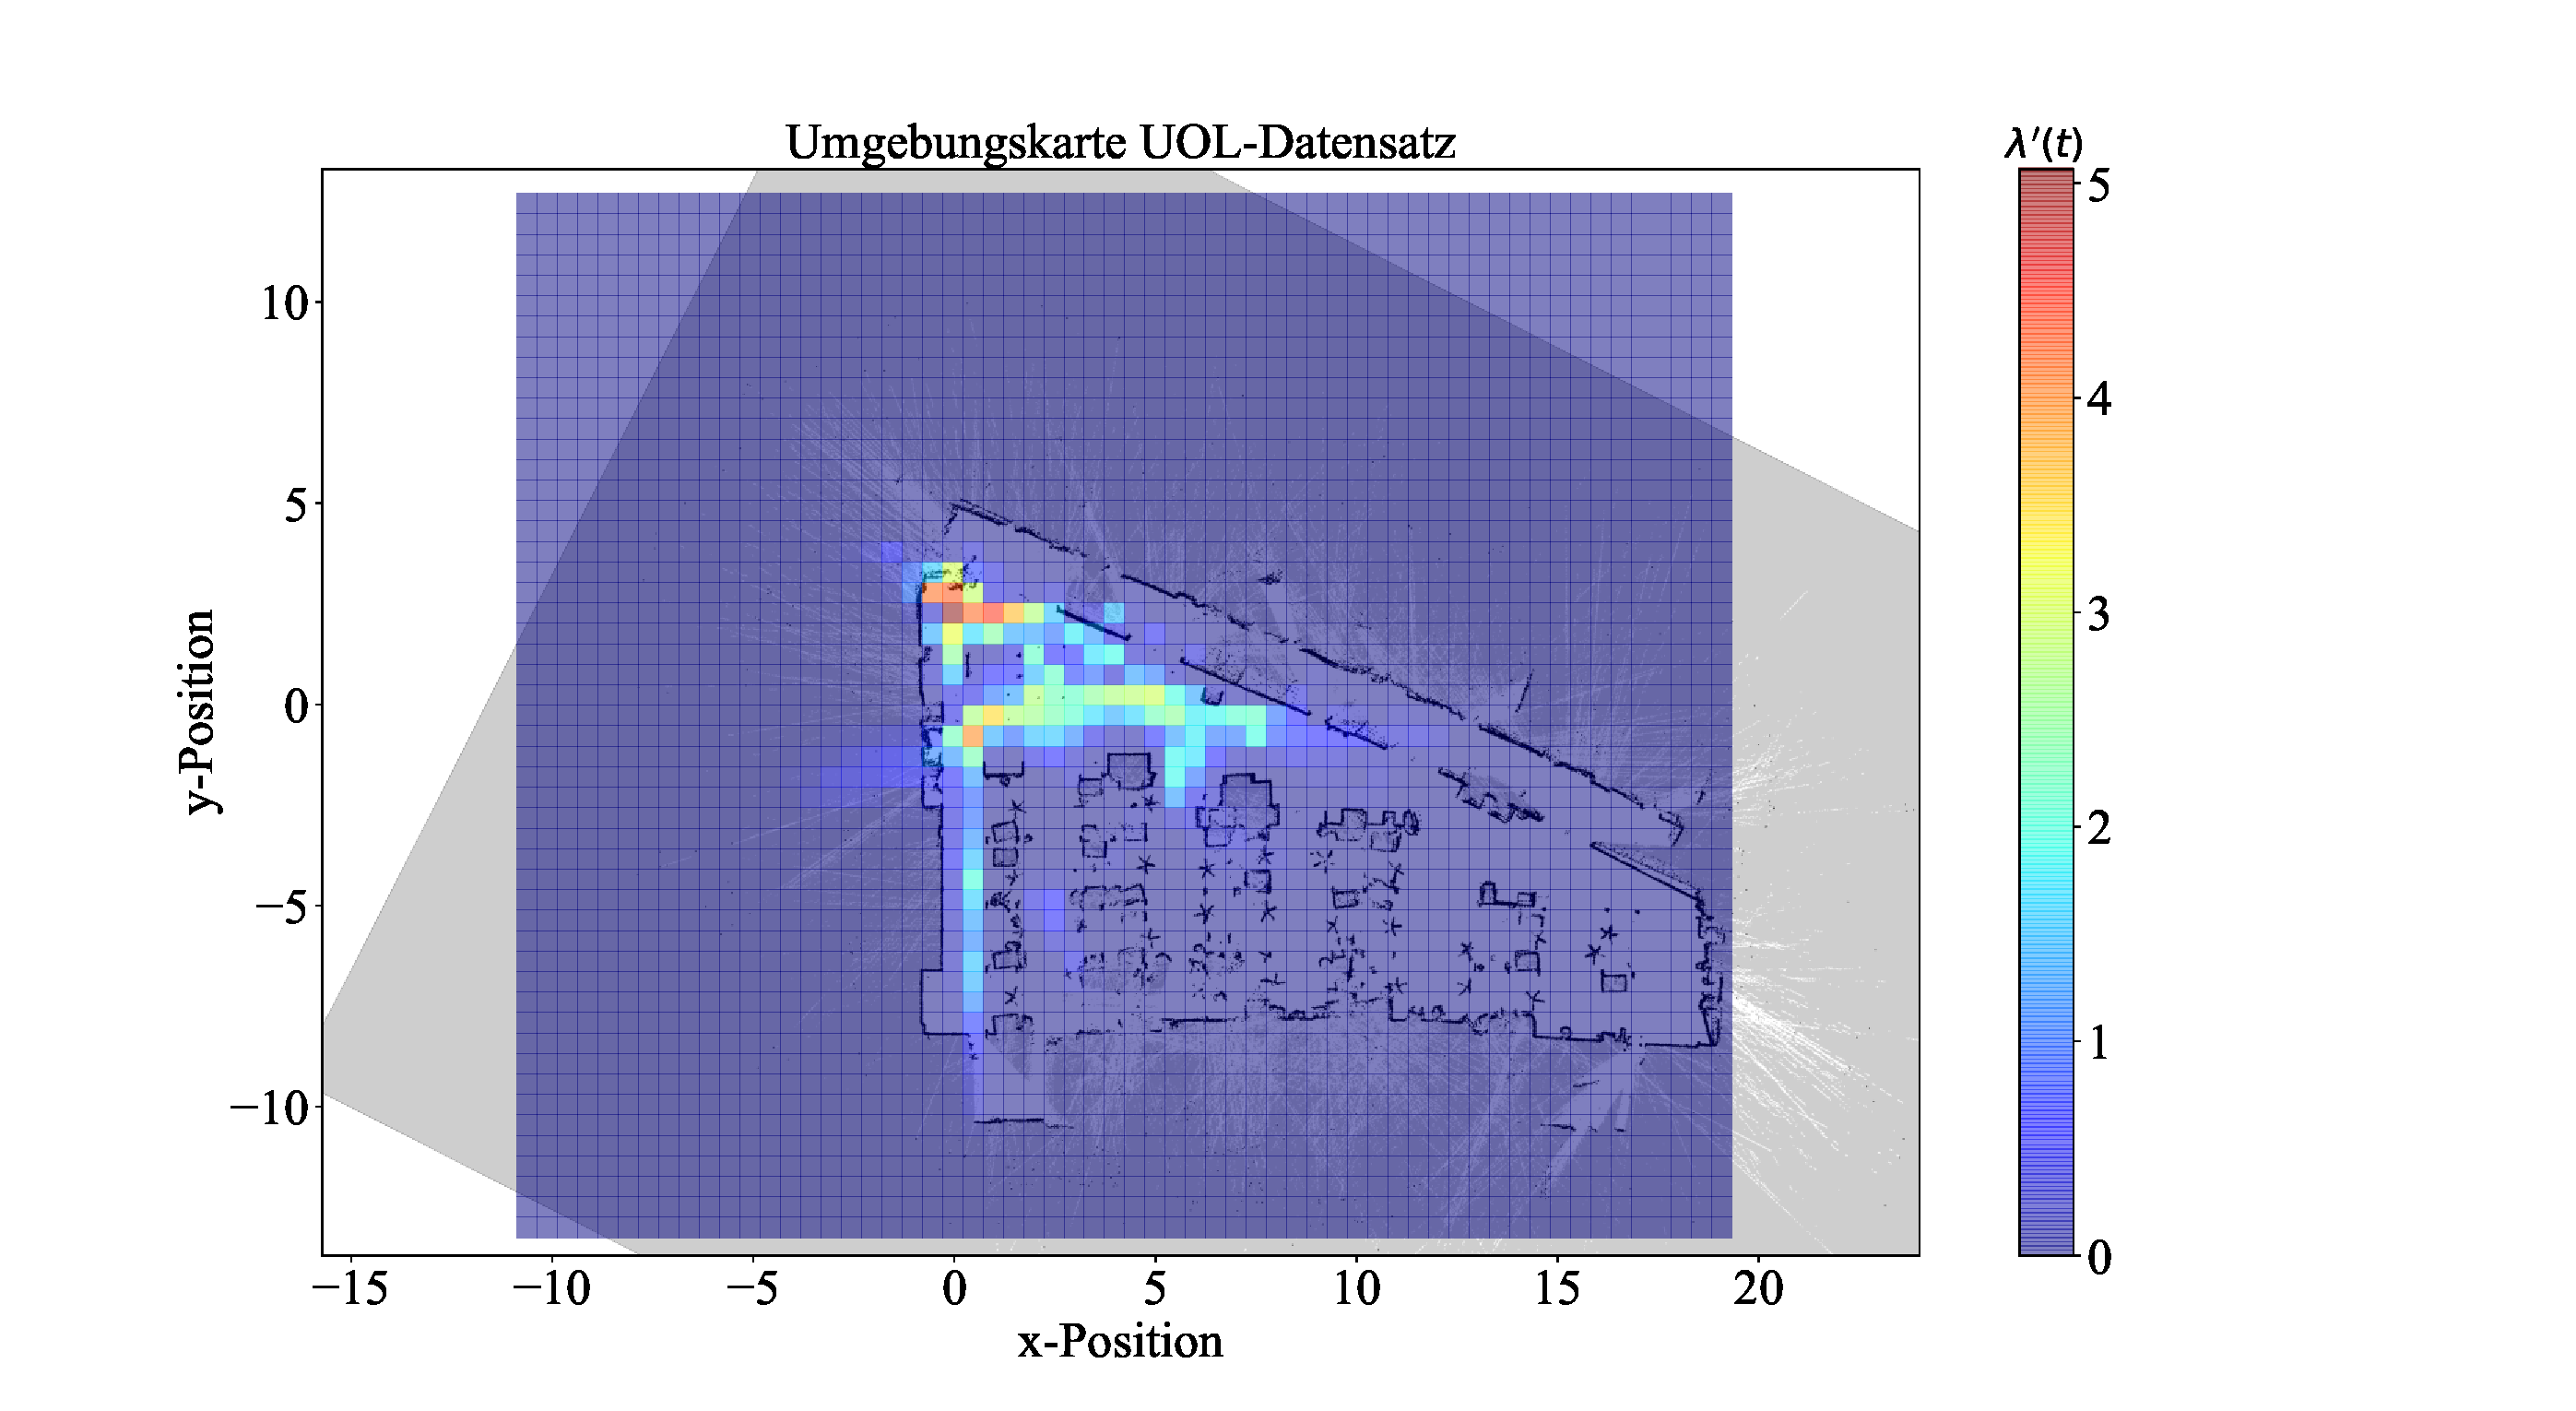
\includegraphics[width=1.0\linewidth]{Abbildungen/evaluation/float_data_best_prediction}}
	
	\subfigure[Prognostizierte Personenraten $\lambda'(t)$ mit statischen Modellen\label{fig.float_static}]{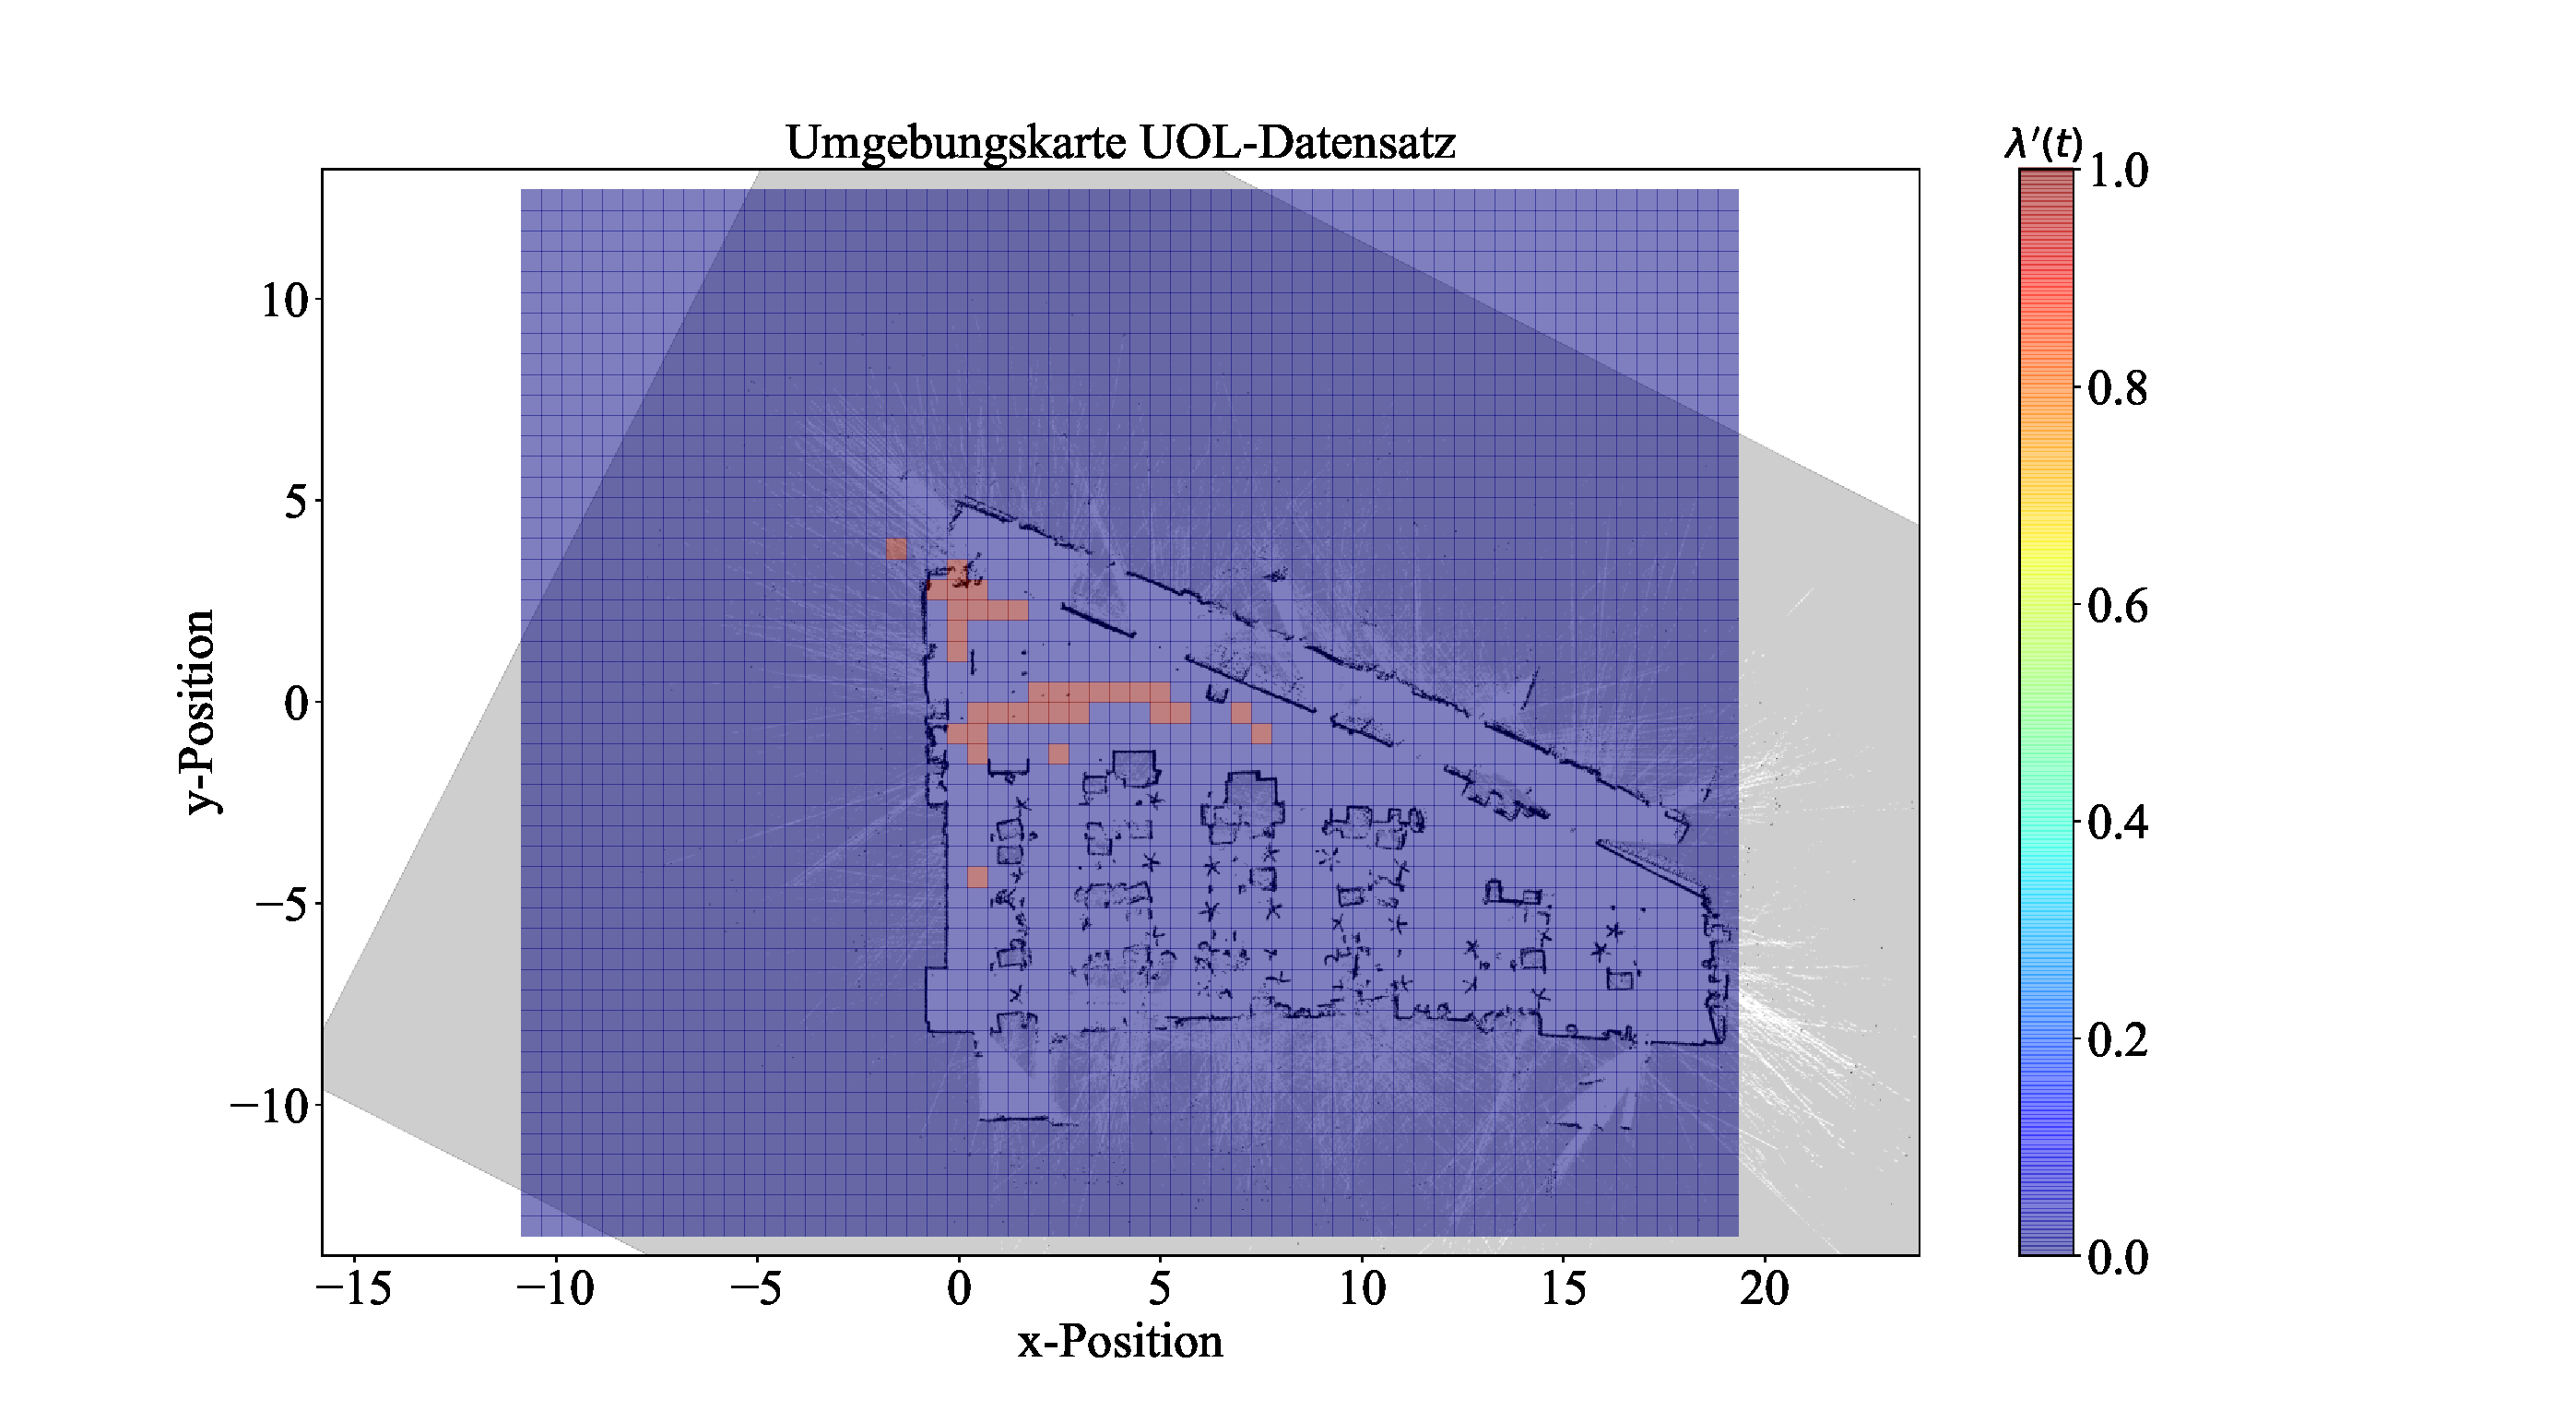
\includegraphics[width=1.0\linewidth]{Abbildungen/evaluation/float_data_static}}
	\caption{Vergleich von FreMEn-Modellen mit statischen Modellen für den quantitativen Fall}
	\label{fig.float_fremen_vs_static}
\end{figure}

Zu erkennen ist, wie schon im Fall binärer Modelle (Abschnitt \ref{sec.Binäres Modell}), dass die FreMEn-Modelle erneut nur in einem Teil der Zellen, in welchen innerhalb des Zeitintervall $\Delta t_i$ Personenraten vorlagen, diese auch prognostizieren. Der Trend der Konzentration hoher Personenraten $\lambda (t)$ innerhalb der Zellen der oberen linken Ecke des Bürogebäudes wird jedoch abgebildet. Vereinzelt werden auch außerhalb des Bürogebäudes Zellen mit Personenraten größer als null prognostiziert. Im Vergleich zu \bild{original_float_data} mit einer maximalen Personenrate von $\lambda_\ind{max} (t) = 10$ beträgt die maximale prognostizierte Personenrate mittels der FreMEn-Modelle $\lambda'_\ind{max} (t) = 5$ (vgl. Bild \ref{fig.float_best_prediction}). Betrachtet man die prognostizierten Personenrate der statischen Modelle (Bild \ref{fig.float_static}), so ergeben sich dort die maximalen prognostizierten Personenraten zu $\lambda'_\ind{max} (t) = 1$. Die Zellen, für welche Personenraten größer als null prognostiziert werden, befinden sich in der linken, oberen Ecke des Bürogebäudes. Verglichen mit den tatsächlichen Personenraten $\lambda (t)$ aus \bild{original_float_data} bilden die FreMEn-Modelle diese deutlich genauer ab als die statischen Modelle.


    	\chapter{Diskussion und Ausblick}
\label{sec.diskussion_und_ausblick}
In dieser Arbeit erfolgt die Darstellung von Personen-Auftrittswahrscheinlichkeiten mittels einer frequenzbasierten Modellierung. Zu diesem Zweck wird eine Server-Client-Struktur mit spezifischer Aufgabenverteilung geschaffen. Den Ausgangspunkt des Modells bilden dabei Personendetektionen innerhalb eines Belegungsgitters, welches in einzelne Zellen unterteilt wird. Die Zellinformationen werden in einer dezentralen Datenbank in einem standardisierten Format gespeichert. Die Datenbankeinträge enthalten neben dem Zeitstempel des Intervalls die korrespondierende Anzahl an Personendetektionen. Es wird eine Verbindung zwischen dem Client und der Datenbank erstellt. Die Daten werden vom Client eingelesen und je nach betrachtetem Modell, welches dem binären oder dem quantitativen Fall entspricht, aufbereitet. Basierend darauf wird das zugrunde liegende Belegungsgitter rekonstruiert. Die Daten werden in einem weiteren Schritt in einen Trainings- und Testdatensatz eingeteilt und an den Server geschickt. Auf diesem erfolgt eine Untersuchung der Frequenzspektren der Daten. Für jede Zelle des Belegungsgitters wird ein separates Modell erstellt. Mittels der FreMEn-Methode wird eine vorher festgelegte Anzahl an prominenten Frequenzen identifiziert und zur Rekonstruktion der Personendetektions-Daten verwendet. Die Evaluation dieses rekonstruierten Modells erfolgt anhand eines Testdatensatzes, welcher nicht zur Erstellung des Modells verwendet wird. Sowohl für den binären wie auch den quantitativen Fall kann durch die Modellierung der Personen-Auftrittswahrscheinlichkeiten durch eine Superposition periodischer Funktionen eine Genauigkeitssteigerung gegenüber statischen Modellen, welche die Personen-Auftrittswahrscheinlichkeiten als zeitlich konstante Funktion approximieren, nachgewiesen werden. Die Höhe der Genauigkeitssteigerung variiert dabei jedoch stark je nach betrachtetem Datensatz. Für binäre Modelle kann eine Genauigkeitssteigerung von bis zu 9.02 Prozentpunkten erreicht werden (vgl. Tabelle \ref{tab.Prädiktionsfehler aruba_binary}). Es werden jedoch auch Limitationen des Modells sichtbar. Für Zellen, welche eine geringe Anzahl an Personendetektionen vorweisen, können mit einer maximalen Anzahl periodischer Prozesse von $l_\ind{max} = 20$ diese hochfrequenten Ereignisse nicht modelliert werden. Eine weitere Erhöhung der Anzahl periodischer Prozesse resultiert in einem Verlust der Generalisierungsfähigkeit des Modells für Daten, welche nicht zur Modellerstellung verwendet werden. Zellen, für welche beispielsweise nur innerhalb von fünf Prozent aller Zeitintervalle Personendetektionen ermittelt werden, werden durch das statische Modell bereits mit einer Genauigkeit von bis zu 95 \% dargestellt. Eine frequenzbasierte Modellierung der Personen-Auftrittswahrscheinlichkeiten ist demnach nur auf Zellen anwendbar, welche eine gewisse Häufigkeit an Personendetektionen aufweisen. \\
Auch für den quantitativen Fall kann durch eine frequenzbasierte Modellierung der Personenraten $\lambda$ eine Steigerung der Prädiktionsgenauigkeit gegenüber einer statischen Modellierung erreicht werden. Erneut ist die Höhe der Genauigkeitssteigerung stark vom jeweils betrachteten Datensatz abhängig. Gegenüber dem statischen Modell kann der Prädiktionsfehler um bis zu 19.94 \% reduziert werden (vgl. Tabelle \ref{tab.Prädiktionsfehler aruba_float}). \\
Im Hinblick auf die frequenzbasierte Modellierung zur Prädiktion von Auftrittswahrscheinlichkeiten von Personen ergeben sich weiterführende Fragestellungen.
So ist eine zeitliche Aktualisierung des Modells nötig. Einen Lösungsansatz stellt hierfür die Neuberechnung des Modells in festgeschriebenen Intervallen dar. So können die Modelle in einem wöchentlichen Takt unter Berücksichtigung von neuen, vom Roboter aufgezeichneten Daten, aktualisiert werden. Als Trainingsdaten könnten hierfür beispielsweise die Detektionen der letzten Wochen $[n, \dots, n -l]$ benutzt werden. Die Evaluierung erfolgt dann anhand der Daten der letzten $l$ Wochen. \\
Eine weitere Fragestellung bildet die Unvollständigkeit der Detektionsdaten. Für die in dieser Arbeit behandelten Datensätze konnte der mobile Roboter die gesamte Umgebung $\mathcal{U}$ überblicken. Die von ihm aufgezeichneten Informationen des zeitlichen Verlaufes der Belegtheit, bzw. Nichtbelegtheit von Zellen, ist also vollständig. In der Realität kann der Roboter die Umgebung jedoch nicht vollständig überblicken, des Weiteren steht eine dauerhafte statische Positionierung zum Aufnehmen von Personendetektionen im Widerspruch der weiteren Aufgaben eines Service-Roboters. Die Aufenthaltsdauer des Roboters auf dem Umgebungsgebiet ist ungleich verteilt. Für Bereiche mit einem längeren Aufenthalt kann eine genauere Schätzung der Personen-Auftrittswahrscheinlichkeiten abgegeben werden als für Bereiche, in denen sich der Roboter nur selten aufhält. \\
Die Unvollständigkeit der Daten ist durch eine geeignete Modellierung abzubilden. Da für unterschiedliche Umgebungsbereiche durch eine ungleich verteilte Menge an aufgenommenen Daten verschiedene Konfidenzbereiche für die Schätzung der tatsächlichen Personendaten existieren, muss eine Entscheidungsregel gefunden werden, anhand derer ein Wert innerhalb des Konfidenzbereiches als Punktschätzung gewählt wird. Die so ermittelten Daten bilden dann erneut die Eingangsgrößen des in dieser Arbeit vorgestellten Modells ab. 
    	Das zwölfwöchige Pflichtpraktikum wurde in der Abteilung ADAS Driving Functions/ Chauffeur Functions der Firma Continental Teves AG \& Co. oHG in Eschborn absolviert. Im Folgenden wird zu Beginn eine Übersicht der Tätigkeitsfelder der Abteilung, in welcher das Praktikum unter Bearbeitung interdisziplinärer Tätigkeitsfelder absolviert wurde, gegeben, bevor darauf folgend die Aufgaben und Tätigkeiten, welche während des Praktikums bearbeitet wurden, beschrieben werden. 

Die Abteilung ist im Bereich des automatisierten Fahrens tätig. Das automatisierte Fahren lässt sich hierbei nach SAE-Standard J3016 in insgesamt fünf Automatisierungsgrade unterteilen. Beschreibt der Automatisierungsgrad des Levels 0 einen Zustand, in dem der Fahrer selbst fährt und im Zuge dessen alle Manöver wie Beschleinigung oder Bremsung selbst durchführt, so handelt es sich bei dem Automatisierungsgrad des Level 5 um einen komplett autonomen Zustand, in welchem der Fahrer keinerlei Beitrag zum Kontrollieren des Fahrzeugs leistet, außer die Vorgabe des Fahrziels sowie des Starten des Systems [Quelle: xxx]. Die Abteilung, in welcher das Pflichtpraktikum absolviert wurde, ist in diesem Kontext innerhalb des Automatisierungsgrades Level 2+ anzusiedeln. Funktionen wie automatisches Einparken, Spurhalten, Abbremsen auf andere Verkehrsteilnehmer sind hier im Fahrzeug integriert. Ebenso sind Fahrfunktionen wie ACC (Adaptive Cruise Control), welches einen konstanten Abstand zu vor dem eigenen Fahrzeug befindlichen Verkehrsteilnehmern in Abhängigkeit ihrer Geschwindigkeiten einhält. Ein besonderer Arbeitsschwerpunkt der Abteilung liegt auf dem automatisierten Spurwechsel, welcher laut SAE-Standard J3016 formell im Automatisierungsgrad Level 3 anzuordnen ist.

Praktikumstätigkeiten
Der erste Einsatzbereich fand im Bereich des automatisierten Spurwechsels im High-Way-Kontext, also auf der Autobahn, statt. Im Folgenden wird die ebenfalls in der Abteilung verwendete Fachsprache benutzt, die verwendeten Abkürzungen werden bei der ersten Erwähnung erläutert und finden sich des Weiteren im Abkürzungsverzeichnis dieses Berichtes (siehe Abkürzungsverzeichnis). Das Vehikel, für welches die automatisierten Funktionen implementiert werden sollen, wird als Ego bezeichnet. Andere Verkehrsteilnehmer werden mit TPO (Traffic Participant Object) gekennzeichnet. Eine Fahrspur wird mit dem Begriff Lane betitelt, die die Lane jeweils nach rechts und links begrenzenden Fahrbahnmarkierungen entsprechend mit Lane-Marker. Die Fahrspur, auf dem sich das Ego-Fahrzeug aktuell befindet, wird mit Ego-Lane bezeichnet. Im Kontext eines geplanten Fahrspurwechsels erhält die Fahrspur, die als Ergebnis des Spurwechsels dient, den Namen Target-Lane. Das erste betrachtete Szenario umfasst ein Ego-Fahrzeug, welches sich zum Startzeitpunkt auf der rechten Spur einer zweispurigen Autobahn befindet. Vor dem Ego-Fahrzeug befindet sich auf der rechten Spur ein TPO. Der Set-Speed, also die gewollte Geschwindigkeit, beträgt 100 km/h. Da das TPO auf der Ego-Lane jedoch nur eine Geschwindigkeit von 80 km/h vorweist, fährt das Ego mit aktiviertem ACC mit konstantem Abstand hinter dem TPO her. Auf der Target-Lane befindet sich ebenfalls ein TPO, welches mit konstanten 80 km/h fährt. Der Wunsch eines Fahrspurwechsels wird, wie bereits erwähnt, durch das Setzen des Blinkers in die gewünschte Richtung signalisiert. Darauf folgend wird unter zu Hilfe nahme der Umgebung eine abzufahrende Bahn geplant. Da diese Bahn keine visuellen Informationen bereitstellt, erfolgte eine solche Visualisierung in einem ersten Schritt innerhalb des Praktikums. Mittels der Programmiersprache Python wurde das anfangs beschriebene High-Way-Szenarion simuliert und visualisert. Ein erstes Konzept der Visualisierung ist in Abbildung xy zu sehen. 

\begin{figure}[!ht]
	\begin{center}
		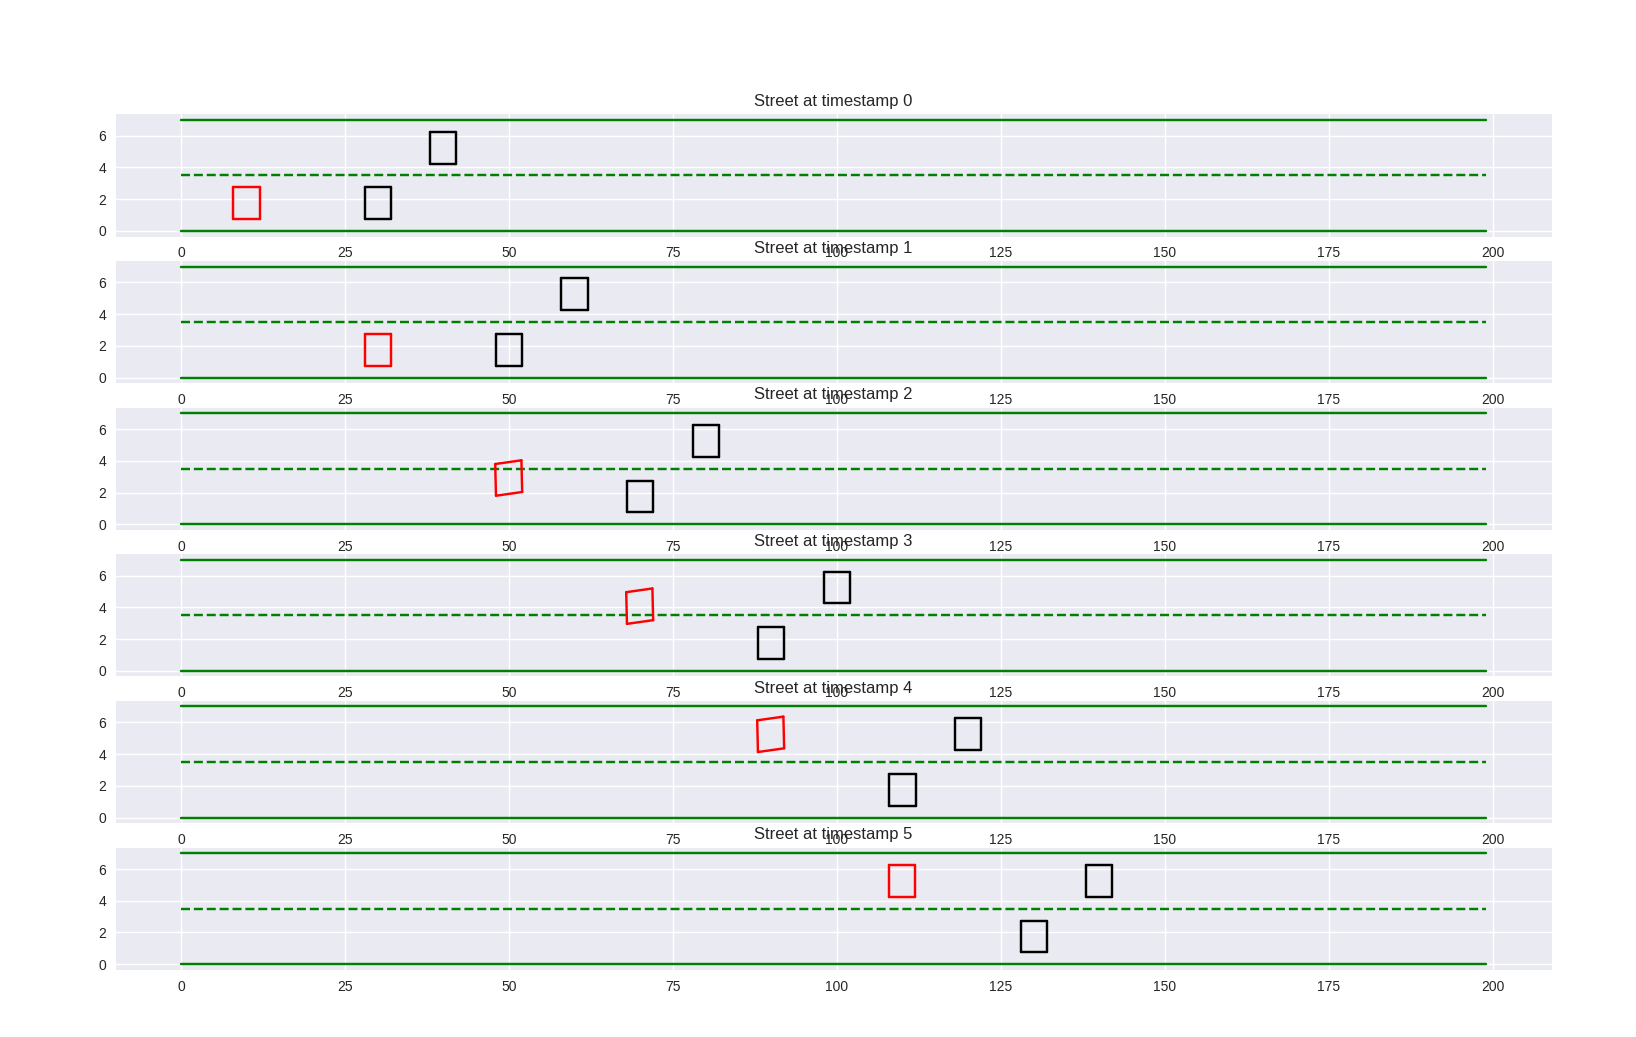
\includegraphics[width=0.8\linewidth]{Abbildungen/bericht/lanechange_visualization}
		\caption{Visualisierung Highway-Spurwechsel in Python}
		\label{fig.highway_spurwechsel_python}
	\end{center}
\end{figure} 

In rot dargestellt sind hier die schemenhaften Umrisse des Ego-Fahrzeuges, in schwarz dargestellt sind die TPO's auf der Ego-Lane sowie auf der Target-Lane. Über mehrere Zeitschritte hinweg ist die Veränderung der Position sowie der Orientierung der Verkehrsteilnehmer während des Spurwechsels aufgetragen. Die Lane-Marker sind im Diagramm in grün eingezeichnet. 
In einem nächsten Schritt erfolgte die Portierung des Visualisierungskonzeptes von der Programmiersprache Python in die Programmiersprache C++. Diese Portierung wurde durch die Tatsache, dass die Planungsalgorithmen für den Spurwechsel ebenfalls in C++ geschrieben sind.

% Kann man hier ggf noch ein Bild von der Gesamtübersicht reinpacken, wie z.B. von dem Eingang der Sensordaten etc? Frank fragen.

Ein weiterer Grund für die Portierung ergibt sich daraus, dass die Datentypen, welche in der urpsprünglichen Python-Visualisierung noch selbst erstellt waren, nun auf die von den tatsächlichen Algorithmen verwendeten Datentypen angepasst werden mussten. Bild xy stellt die fertige Visualisierung dar, der Übersichtlichkeit halber sind nur zehn Zeitschritte des Spurwechsels dargestellt. Im Gegensatz zu Bild xy ist die C++ - Portierung um einige Funktionalitäten ergänzt.

		%\chapter{Tipps zur Erstellung der Arbeit}
Im Folgenden sind einige Tipps zur schriftlichen Ausarbeitung zu finden, z.\,B. zur korrekten Darstellung von Gleichungen und Grafiken oder zum Bezug der dazu notwendigen Software. Grundsätzlich lassen sich unter folgendem Link Hilfestellungen zu den meisten Problemen bei der Erstellung Arbeit finden: http://bfy.tw/Bq9t

%%%%%%%%%%%%%%%%%%%%%%%%%%%%%%%%%%%%%%%%%%%%%%%%%%%%%%%%%%%%%%%%%%%%%%%%%%%%%%%%%%%%

\section{Darstellung von Gleichungen}
\label{sec.Gleichungen}
Der am imes verwendete Formelsatz entspricht der DIN 1338 und lässt sich auch in sämtlichen Skripten des imes wiederfinden, \zB in Robotik I, Robotik II oder Mechatronische Systeme.

Grundsätzlich gilt: Variablennamen werden kursiv gesetzt (auch wenn diese als Index benutzt werden, \zB $a_i$), beschreibende Indizes (z.\,B. $b_\ind{Reifen}$ oder $b_\ind{R}$) und allgemeine Funktionen (\zB Sinus- oder e-Funktion) aufrecht:

\begin{equation}
\label{eq:bsp_1}
	f(t) = \int\limits_{t_\ind{start}}^{t_\ind{end}} \sin(\omega t) \ind{d}t.
\end{equation}

Bei der ersten Verwendung von Variablen sollten diese unmittelbar vor oder nach der Gleichung im Text erläutert werden, in diesem Fall die exemplarische Funktion $f(t)$, Start- und Endzeitpunkt $t_\ind{start}$ bzw. $t_\ind{end}$, Kreisfrequenz $\omega$ und Zeit $t$. 


Matrizen und Vektoren werden fett gedruckt dargestellt. Matrizen werden mit großen, Vektoren mit kleinen Buchstaben bezeichnet. In der Gleichung

\begin{equation}
\label{eq:bsp_2}
	\boldsymbol{q} = (q_1, q_2, ..., q_n)^\mathrm{T}
\end{equation}

beschreibt $\boldsymbol{q}$ den Vektor mit allen Gelenkwinkeln, $q_1$ hingegen den Gelenkwinkel der ersten Achse. Zahlreiche weitere Beispiele zur Darstellung von Formeln können in den oben genannten Skripten nachgeschlagen werden.

Weitere Beispiele für korrekten Formelsatz:

\textbf{TODO -> versch. Stellen aus Skripten suchen und Code kopieren}

%%%%%%%%%%%%%%%%%%%%%%%%%%%%%%%%%%%%%%%%%%%%%%%%%%%%%%%%%%%%%%%%%%%%%%%%%%%%%%%%%%%%

\section{Darstellung von Grafiken}

Grafiken sollten nach Möglichkeit als Vektorgrafiken (z. B. .eps, .pdf) exportiert und in LaTeX eingebunden werden. Die Schriftart sollte der Schriftart der restlichen Arbeit entsprechen (Times). Die Schriftgröße in der Grafik sollte kleiner oder gleich der Größe des Fließtextes sein (nach eigenem Ermessen, solange die Lesbarkeit noch gegeben ist). Auch bei Abbildungen sind die Formatierungsschriften aus \Sec{Gleichungen} einzuhalten. Ein Beispielplot aus Matlab ist in \bild{Template} dargestellt. Das Skript zur Erstellung des Plots in Matlab ist unter template\_einfach.m zu finden.

\begin{figure}[!ht]
	\begin{center}
		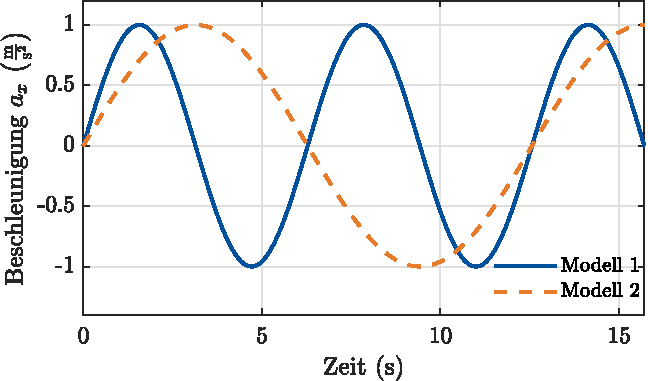
\includegraphics[]{template_einfach}
		\caption{Vergleich der zeitlichen Beschleunigungsverläufe der beiden Modellierungsansätze Hü (blau) und Hott (orange gestrichelt)}
		\label{fig.Template}
	\end{center}
\end{figure}

%%%%%%%%%%%%%%%%%%%%%%%%%%%%%%%%%%%%%%%%%%%%%%%%%%%%%%%%%%%%%%%%%%%%%%%%%%%%%%%%%%%%

\section{Software}
\subsection{Matlab, Corel}
Für Matlab und Corel sind an der Uni Hannover kostenlose Campuslizenzen verfügbar. Anleitungen zum Bezug sind unter https://www.luis.uni-hannover.de/softwarekatalog.html zu finden. Für Corel existiert am imes ein Plugin zur Nutzung von LaTeX-Befehlen. Das Plugin und die zugehörige Anleitung sind im Vorlagenordner zu finden. Alternativ zu Corel kann auch die freie Software Inkscape genutzt werden (https://inkscape.org).

\subsection{LaTeX}
Vorschläge für TeX-Distributionen:
\begin{itemize}
	\item MiKTeX (Windows): https://miktex.org/
	\item TeXLive (allg.): http://www.tug.org/texlive/
\end{itemize}

Vorschläge für Texteditoren:
\begin{itemize}
	\item TeXnicCenter (Windows): http://www.texniccenter.org/
	\item TeXMaker (allg.): http://www.xm1math.net/texmaker/
\end{itemize}

%%%%%%%%%%%%%%%%%%%%%%%%%%%%%%%%%%%%%%%%%%%%%%%%%%%%%%%%%%%%%%%%%%%%%%%%%%%%%%%%%%%%

\section{Literaturverweise}
Beispiele für Literaturverweise sind im Literaturverzeichnis zu finden, z.\,B. Journalbeitrag \cite{Ber59}, Konferenzbeitrag \cite{Hussong08}, Buch \cite{Wintermantel09}. Sofern nicht explizit anders eingestellt, taucht nur diejenige Literatur im Verzeichnis auf, auf die in der Arbeit verwiesen wird.

%%%%%%%%%%%%%%%%%%%%%%%%%%%%%%%%%%%%%%%%%%%%%%%%%%%%%%%%%%%%%%%%%%%%%%%%%%%%%%%%%%%%

\section{Eigene Befehle in LaTeX}
In LateX können auch eigene Befehle definiert und genutzt werden, \zB zur Verwendung immer wiederkehrender Formelzeichen. So kann beispielsweise ein Koordinatensystem $\ks{A}$ direkt mit dem Befehl \textbackslash ks\{A\} eingefügt werden. Eine Liste der Befehle ist in der Datei befehle.sty zu finden.


		%\chapter{Betreuer- und/oder projektspezifische Anmerkungen}
Für Ergänzungen zur Vorlage, die nicht allgemeingültig sind, bitte ausschließlich dieses Kapitel nutzen!

ToDos für die Vorlage:
\begin{itemize}
	\item Aufgabenstellung direkt ins Dokument, Platzhalter-pdf, manuell reinsortieren?
	\item mehr Beispiele für Formelsatz aus versch. Skripten reinkopieren
	\item Befehle.sty erläutern
\end{itemize}
		%\chapter{(Beispielkapitel) Robotersysteme}

Das folgende Kapitel soll als Beispielkapitel dienen. Nach der Kapitelüberschrift wird der Kapitelinhalt in ein paar Sätzen beschrieben.
Hier steht weiterer Text.

\section{PR2}

Der PR2 (Willow Garage Inc., Menlo Park, USA) ist ein \textbf{\textit{menschenähnlicher}} Serviceroboter, der seinen Dienst in Wohnräumen verrichten soll und derzeit im sogenannten PR2 Beta-Programm von elf Forschungseinrichtungen über einen Zeitraum von zwei Jahren getestet wird 
\cite{WillowGarage2010}.
Hier steht weiterer Text.  d

\begin{figure}[!ht]
	\centering
	\subfigure[]{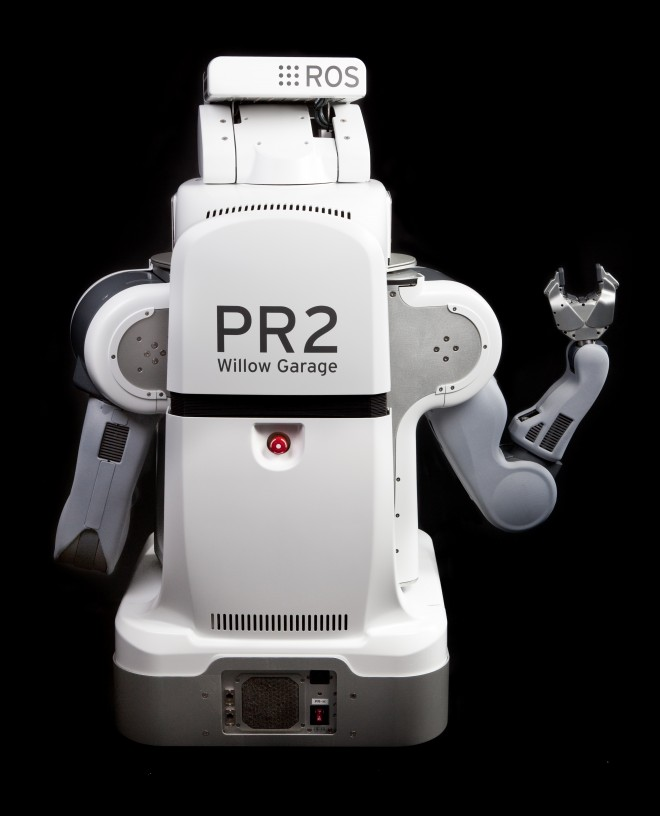
\includegraphics[height=50mm]{PR2-1}}
	\hspace{5mm}
	\subfigure[]{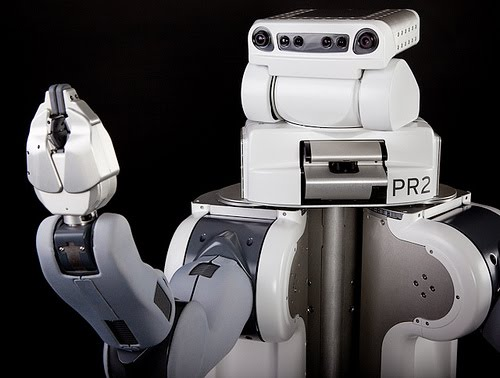
\includegraphics[height=50mm]{PR2-2}}
	\hspace{5mm}
	\subfigure[]{\includegraphics[height=50mm]{PR2-3}}
	\caption{Serviceroboter PR2 von Willow Garage (Quelle: Willow Garage))}
	\label{fig.PR2}
\end{figure}

Ausgestattet ist der PR2 mit zwei Armen, die jeweils sieben Freiheitsgrade haben und an deren Enden ein Greifer montiert ist, siehe \bild{PR2}. Die Sensorik des Armes besteht aus einer Kamera am Unterarm und Druck- sowie Beschleunigungssensoren am Greifer. Die Nutzlast eines Arms ist mit \SI{1,8}{kg} ausgewiesen. Weiterhin verfügt der Roboter über einen dreh- und schwenkbaren Kopf, in dem eine 5-Megapixel Farbkamera, ein LED-Texturprojektor und zwei Stereokameras integriert sind, wobei eine Kamera für die Fernsicht und die andere für die Objektmanipulation genutzt wird. Unterhalb des Kopfes ist ein schwenkbarer Laserscanner und ein Inertialsensor verbaut. Die Position des Oberkörpers lässt sich in der Höhe zwischen \SI{1330}{mm} und \SI{1645}{mm} (Gesamthöhe) variieren. Angetrieben wird die omnidirektionale Basis von vier gelenkten Rädern, die eine maximale Geschwindigkeit von \SI{3,6}{\kilo\metre\per\hour} ermöglichen. Die quadratische Basis hat eine Kantenlänge von \SI{668}{mm}. Als Recheneinheit stehen zwei Server zur Verfügung, die jeweils auf acht CPU-Kernen rechnen und dabei auf 24\,GB Arbeitsspeicher zugreifen können. Als Betriebssystem wird Ubuntu verwendet, auf dem das Robot Operating System, kurz ROS, die Grundlage für die Datenverarbeitung bildet. Da ROS innerhalb dieser Arbeit ebenfalls zum Einsatz kommt, wird dieses in \Sec{ROS} vorgestellt und an den entsprechenden Stellen weiter erläutert. Die Kosten für einen PR2-Roboter belaufen sich derzeit auf etwa \SI{400 000}{\text{US-Dollar}}\footnotemark. Mit Hilfe des PR2 wurden von den zuvor erwähnten Beta-Testern Szenarien bewältigt, die innerhalb des menschlichen Wohnraumes auftreten können. An der TU München hat ein PR2-Roboter beispielsweise zusammen mit einem anderen Robotersystem einen Pfannkuchen gebacken \cite{TUM2011}.
\footnotetext{Der angegebene Preis wurde am 16.08.2011 der Website http://www.willowgarage.com/pages/pr2/order entnommen und versteht sich exklusive Steuern und Versandkosten.}

\section{ROS}
\label{sec.ROS}

Hier steht weiterer Text.

\begin{table}
	\centering
	\caption{Technische Daten der youBot Plattform}\label{tab.TechSpecYouBotBase}
	\vspace*{-3mm}
	\begin{tabular}{lcr}
        \toprule
		Bezeichnung		& Formelzeichen	&              \\
		\midrule
		Gesamtlänge 	& $a$           & \SI{530}{mm} \\
		\rowcolor{Snow2}
		Gesamtbreite 	& $b$           & \SI{350}{mm} \\
		Höhe			& $h$           & \SI{106}{mm} \\
		Radstand		& $l$           & \SI{470}{mm} \\
		\bottomrule
	\end{tabular} 
\end{table}

\begin{lstlisting}[label=source.launchHokuyo,caption=Launchfile zum Start der hokuyo\_node]
<!-- launch hokuyo node -->
<node pkg="hokuyo_node" type="hokuyo_node" name="hokuyo_node" output="screen">
	<param name="port" value="/dev/ttyACM0"/>
	<param name="frame_id" value="/base_laser_front_link"/>
</node>
\end{lstlisting}

    %\nocite{*}                             % alle Literaturquellen einbinden, sonst werden nur die zitierten
                                            % Quellen im Literaturverzeichnis angezeigt (ist Geschmackssache).
                                            % eher nicht verwenden, außer man hat einen guten Grund
    %\appendix                               % Anhang starten, jedes weitere Kapitel bekommt jetzt einen Buchstaben
    %\chapter*{Anhang}                       % Anhang als Chapter
    %\addcontentsline{toc}{chapter}{Anhang}
    %\thispagestyle{empty}                   % keine Kopfzeile, Seitenzahl u.a., leere Seite mit Überschrift Anhang
    %\setcounter{chapter}{1}                 % Chapter Counter auf 1 = im Anhang A
    %\setcounter{equation}{0}                % Equation Counter nullen
    %\newpage                                
    %\ihead{\normalfont Anhang}              % Kopfzeile auf Anhang setzen



    %% --- Ab hier der Anhang einfügen

    %\include{anhang_wheatstone}            % Anhang
    %\include{anhang_fehlerfortpflanzung}
		%\include{anhang_mgcEinstellungen}
		%\include{anhang_trafos}
		%\include{anhang_befestigen}
		%\include{anhang_datenblaetter}
    %% --- Anhang zu Ende
		
    \ihead{\normalfont\headmark}            % kolumnentitel innen
 
    %% --- Literaturverzeichnis
    \bibliographystyle{alphadin}
    \bibliography{Vorlagen/masterbib}

\end{spacing}
\end{document}                              % fertig!

